\definecolor{c15blue}{HTML}{2A78D6}
\definecolor{c15orange}{HTML}{EB6834}
\definecolor{c15aqua}{HTML}{1BAF7A}
\definecolor{c15gray}{HTML}{52514E}

\chapter{Identification and Estimation of Single-Object Auctions}\label{ch:auction-empirics}
\chaptermark{Estimating Single-Object Auctions}

Auctions are the setting in which the structural program of empirical industrial organization, outlined in
\cref{ch:intro}, works best. In
\cref{ch:conduct} the way firms compete was itself unknown, so conduct entered the model as a parameter to be
estimated. In an auction the seller writes down the rules. The researcher knows who wins and what each bidder
pays as a function of the bids. The only behavioral assumption left is that bidders play an equilibrium
\citep[Section~1]{AtheyHaile2007}. \Cref{ch:auction-theory} derived how bidders behave, given the joint
distribution of their values and information. This chapter runs the argument in reverse. It asks what observed
bids reveal about the distribution that generated them and how to estimate that distribution. It then uses
the estimates to answer questions about reserve prices, auction formats, entry and collusion.

The central idea fits in one display. In a first-price auction with $n$ symmetric bidders whose values are
independent, let $G$ and $g$ be the distribution and density of a rival's bid. A bidder who bids $b$ must then
have the value
\[
v=b+\frac{G(b)}{(n-1)\,g(b)} .
\]
The right side involves only the bid and the distribution of bids, which the data reveal. Each bid therefore
maps into the value that rationalizes it, and no equilibrium needs to be computed. The formula is the auction
counterpart of recovering marginal cost from a pricing first-order condition once demand has been estimated
(\cref{ch:diffprod,ch:blp}). Here the distribution of rival bids plays the role of the demand curve. Much of the
chapter extends this inversion to richer models and asks what remains identified when the data are poorer.

Five questions organize the chapter. Which primitives are identified from which data? How should they be
estimated, and how fast do the estimators converge? How can the information structure be tested, in particular
private against common values? How should we handle heterogeneity that bidders see and the econometrician does
not, and participation that responds to the auction's features? What does a complete application look like,
from reduced-form evidence to counterfactual policy?

The chapter is organized as follows. \Cref{sec:15-approach} defines the primitives, the observables, and what
identification and testability mean. \Cref{sec:15-ascending} treats second-price and ascending auctions, where
bids equal values but some bids are never observed. It also covers the bounds that survive when the button
model of the English auction fails. \Cref{sec:15-direct,sec:15-gpv} turn to first-price auctions. The first
studies direct parametric methods and the simulated estimator of \citet{LaffontOssardVuong1995}. The second
develops the indirect approach of \citet{GuerrePerrigneVuong2000} in full. \Cref{sec:15-apv,sec:15-cv,sec:15-uh,sec:15-entry}
relax the maintained assumptions one at a time. They cover affiliated and asymmetric private values, common
values, unobserved auction heterogeneity, and entry, dynamics and risk aversion. \Cref{sec:15-als} then follows
the timber study of \citet{AtheyLevinSeira2011} from question to counterfactuals. \Cref{sec:15-collusion} reviews
tests for collusion and the auction designs that make bidding rings harder to run. \Cref{sec:15-divisible}
turns to divisible goods, such as Treasury bills and central bank loans, for which bidders submit demand
schedules. \Cref{sec:15-synthesis} collects the identification results in one map.
\Cref{tab:15-roadmap} summarizes the plan. Apart from the short treatment of divisible goods in
\cref{sec:15-divisible}, this book treats single-unit auctions only. Auctions of several different objects,
such as spectrum licenses, raise separate problems.

The chapter leans on the rest of the book in several places. \Cref{ch:auction-theory} supplies the equilibrium
theory, and we recall its results by reference instead of deriving them again. The analysis of bidding rings
connects to the cartel theory of \cref{ch:collusion-theory} and to the bid-rigging and knockout studies of
\cref{ch:collusion-evidence}. \Cref{app:econometrics} reviews the econometric tools used here, including kernel
density estimation, the delta method, the bootstrap, simulation estimators and matching. \Cref{app:math}
collects the results on order statistics, characteristic functions, affiliation and log-concavity. Most
sections close with the empirical magnitudes found in timber, procurement and offshore oil auctions. For
studies that we summarize without a full treatment, we rely on the survey of \citet{HortacsuPerrigne2021}
and cite its pages.

\section{The Structural Approach to Auction Data}\label{sec:15-approach}

This section sets up the framework that the rest of the chapter uses. It defines the primitives and the
observables, states the sampling assumptions, gives precise definitions of identification and testability, and
previews the two broad estimation strategies that the later sections develop.

Auctions suit this program for the reasons given in \cref{sec:14-why-data}. Bids, prices, the number of bidders
and often the identities of the bidders are recorded. Above all, the seller writes down the rules, so the mapping
from bids to the allocation and to payments is known to the researcher. \citet[Section~1]{AtheyHaile2007} observe
that the primitives of any strategic model are the players, the information structure, the rules of play and the
players' objectives. In auction markets these elements can be described with unusual confidence. The only
behavioral assumption left is equilibrium play.

The structural approach targets questions that bids alone cannot answer. \citet[Section~1]{AtheyHaile2007} list
several. Some concern the division of rents in auctions of public resources, the adequacy of reserve prices in
government auctions, and the effects of mergers between bidders on procurement costs. The last is a merger
simulation of the kind studied in \cref{ch:mergers}, with the advantage that the game form is known. Others concern the
revenue consequences of changing the auction rules, the efficiency of bundling procurement contracts and the value
of seller reputations. Still others concern information-acquisition costs, adverse selection created by private
information, and risk aversion. Each question needs the distribution functions that describe bidders' demand and information. They
add a methodological point. Economic theory shapes many parts of an empirical model, but it rarely says anything
about the distributions of unobservables. Much of what auction data can teach us does not depend on such
distributional assumptions \citep[Section~1]{AtheyHaile2007}.

\subsection{Primitives and observables}\label{sec:15-primitives}

A single indivisible object is sold to one of $n\ge2$ risk-neutral bidders. Bidder $i$ has a value $V_i$ for the
object and private information summarized by a signal $S_i$. Upper-case letters denote random variables and
lower-case letters their realizations. The general model of \cref{sec:14-info} specifies the joint distribution of
values and signals. The two classes of models in \cref{def:14-private-values} differ in whether a rival's signal
is informative about one's own value. In a \emph{private values} (PV) model it is not, and we normalize $S_i=V_i$.
The primitive is then the joint distribution $F_{\bm V}$ of the vector of values $\bm V=(V_1,\dots,V_n)$. In the
\emph{independent private values} (IPV) model, $F_{\bm V}(\bm v)=\prod_{i=1}^nF_i(v_i)$. In the \emph{symmetric}
IPV model (SIPV), every $F_i$ equals a common $F$ with density $f$. In a \emph{common values} (CV) model a bidder
would revise her expected value if she learned a rival's signal \citep[p.~2110]{AtheyHaile2002}. Its primitive is
the joint distribution of values and signals.

We maintain the setting of \citet[Section~2.1]{AtheyHaile2002} unless a section says otherwise. The number of
bidders is common knowledge and there is no reserve price. Bidders play a Bayesian Nash equilibrium in weakly
undominated strategies, symmetric when bidders are symmetric. Ascending auctions follow the button model of
\cref{def:14-button}, in which bidders exit observably and irrevocably as the price rises.

The data never contain values. \citet[Section~2.2]{AtheyHaile2002} distinguish what is always observed from what is
sometimes observed. The econometrician always sees the number of bidders $n_t$ and the transaction price $P_t$ of
each auction $t$. With asymmetric bidders, the set of participants is also known. The following may or may not be
available:
\begin{enumerate}[label=(\roman*)]
\item bids other than the transaction price,
\item bidder identities, in particular the identity $I_t$ of the winner,
\item \emph{auction covariates} $Z_t$, such as the appraised value of the object or its realized ex post value,
\item \emph{bidder covariates} $W_{it}$, such as firm size, location, distance to the project or backlog.
\end{enumerate}
The format determines which bids exist. A sealed-bid auction can record every bid. A Dutch auction stops at the
first bid, so only the winning bid exists. An ascending auction ends when the next-to-last bidder drops out, so the
price at which the winner would have exited is never revealed (\cref{sec:14-spa-data}).

A last type of information is variation in the number of bidders. Participation is \emph{exogenous} if the joint
distribution of the signals of any subset of bidders does not depend on which other bidders participate
\citep[p.~2113]{AtheyHaile2002}. Exogenous variation arises, for example, when potential bidders draw
participation costs that are independent of their values, when a seller restricts participation, or by design in
field experiments.

Throughout, we observe $T$ auctions indexed by $t=1,\dots,T$, and $T_n$ of them have $n$ bidders. Two sampling
assumptions underlie everything that follows. First, auctions are independent, and the values and signals in each
auction are drawn from the same distribution, conditional on any auction covariates. Second, the same equilibrium
is played in all auctions with the same observables. Without the second assumption, the observed distribution of
rivals' bids would mix several equilibria and would not represent the beliefs of a bidder in any one auction
\citep[footnote~18]{AtheyHaile2007}. Dependence across auctions, such as the effect of a backlog of contracts won
earlier, is excluded here and studied in \cref{sec:15-entry}. Values and bids have continuous distributions, so
ties occur with probability zero. All asymptotic statements let $T\to\infty$, with $T_n\to\infty$ for every $n$ that
is used.

\subsection{Identification and testability}\label{sec:15-identification}

The general notion of identification in \cref{app:econometrics} specializes neatly to auctions. Let $\mathbb F$ be a
set of joint distributions of the latent variables (values and signals). Let $\mathbb H$ be the set of all joint
distributions of the observable variables. Let $\Gamma$ be a collection of mappings $\gamma:\mathbb F\to\mathbb H$.
Each $\gamma$ sends a distribution of primitives to the distribution of observables that equilibrium play in a
given auction game implies. Following \citet[p.~2114]{AtheyHaile2002}, a \emph{model} is a pair $(\mathbb
F,\Gamma)$. Implicit in the specification is the assumption that the model contains the true structure.

\begin{definition}[Identification, \citealp{AtheyHaile2002}]\label{def:15-identified}
A model $(\mathbb F,\Gamma)$ is \emph{identified} if for every $(F,\tilde F)\in\mathbb F^2$ and
$(\gamma,\tilde\gamma)\in\Gamma^2$, the equality $\gamma(F)=\tilde\gamma(\tilde F)$ implies
$(F,\gamma)=(\tilde F,\tilde\gamma)$.
\end{definition}

\begin{definition}[Testability, \citealp{AtheyHaile2002}]\label{def:15-testable}
A model $(\mathbb F,\Gamma)$ is \emph{testable} if $\bigcup_{\gamma\in\Gamma,\,F\in\mathbb F}\gamma(F)\neq\mathbb H$,
that is, if some distributions of observables cannot be generated by the model.
\end{definition}

In most of this chapter $\Gamma$ contains a single mapping, the equilibrium of a given auction game. Identification
then means that the distribution of observables determines $F$ uniquely. A model is \emph{partially identified}
when the observables determine only some features of $F$, or only bounds on it \citep[Section~1]{AtheyHaile2007}.
Testability means that equilibrium behavior in the model places refutable restrictions on the data.

Three remarks clarify how these definitions are used. First, equilibrium bidding is maintained throughout. A
rejection is therefore read as evidence against the assumptions on primitives, such as independence or symmetry.
Equilibrium play itself is never the hypothesis under test \citep[p.~2114]{AtheyHaile2002}. Second, identification and estimation are
distinct questions. Identification asks what the observables could reveal with an infinite sample. Estimation
asks how to approximate that answer in a finite sample, and it may well use parametric families. When a model is
identified nonparametrically, a parametric specification becomes a parsimonious approximation rather than a
maintained hypothesis about the true structure (\citealp[p.~2109]{AtheyHaile2002}, following \citealp{Roehrig1988}).
Third, a
nonidentification result is informative as well. It shows which models generate the same data, and so which
conclusions rest on assumptions rather than on evidence.

\subsection{Two routes from bids to primitives}\label{sec:15-routes}

There are two broad ways to estimate the primitives, and \cref{fig:15-routes} contrasts them. The \emph{direct}
route specifies a parametric family $F(\cdot;\theta)$, solves for the equilibrium bid function $\beta(\cdot;\theta)$,
derives the implied likelihood or moments of the bids, and fits them to the data
\citep{Paarsch1992,DonaldPaarsch1996,LaffontOssardVuong1995}. The \emph{indirect} route of
\citet{GuerrePerrigneVuong2000} starts from the bids. It estimates their distribution, inverts each bidder's
first-order condition to recover the value that rationalizes each bid, and then estimates $F$ from these
\emph{pseudo-values}. In second-price and ascending auctions with private values both routes are simple, because
the bid function is the identity. The difficulty there is that some bids are not observed (\cref{sec:15-ascending}).
In first-price auctions the two routes differ sharply (\cref{sec:15-direct} and \cref{sec:15-gpv}).

\begin{figure}[htbp]
\centering
\begin{tikzpicture}[
  box/.style={draw=c15gray, rounded corners=2pt, align=center, font=\footnotesize, minimum height=1.25cm,
              text width=2.6cm, fill=white},
  arr/.style={-{Stealth[length=2.2mm]}, thick, c15gray},
  lab/.style={font=\scriptsize\itshape, align=center, text width=1.4cm}
]
\node[box] (d1) {parameter\\ $\theta$};
\node[box, right=1.35cm of d1] (d2) {value\\ distribution\\ $F(\cdot;\theta)$};
\node[box, right=1.35cm of d2] (d3) {bid function\\ $\beta(\cdot;\theta)$};
\node[box, right=1.35cm of d3] (d4) {likelihood or\\ moments of bids};
\draw[arr] (d1) -- node[lab, above] {specify} (d2);
\draw[arr] (d2) -- node[lab, above] {solve the equilibrium} (d3);
\draw[arr] (d3) -- node[lab, above] {derive} (d4);
\node[box, below=1.7cm of d1] (i1) {observed bids\\ $b_{it}$};
\node[box, below=1.7cm of d2] (i2) {bid\\ distribution\\ $(\hat G,\hat g)$};
\node[box, below=1.7cm of d3] (i3) {pseudo-values\\ $\hat V_{it}$};
\node[box, below=1.7cm of d4] (i4) {value density\\ $\hat f$};
\draw[arr] (i1) -- node[lab, above] {estimate} (i2);
\draw[arr] (i2) -- node[lab, above] {invert the first-order condition} (i3);
\draw[arr] (i3) -- node[lab, above] {estimate} (i4);
\node[anchor=south west, font=\small\itshape, c15blue] at ([yshift=2pt]d1.north west) {Direct route};
\node[anchor=south west, font=\small\itshape, c15orange] at ([yshift=2pt]i1.north west) {Indirect route};
\draw[densely dashed, c15gray, -{Stealth[length=2mm]}] (i1.east) ++(0,0.25) to[out=20, in=200] node[pos=0.55,
  above, sloped, font=\scriptsize\itshape] {fit to the data} (d4.south west);
\end{tikzpicture}
\caption{Two routes from bids to the value distribution. The direct route solves the equilibrium for every trial
parameter and compares implied and observed bids. The indirect route inverts the bidders' first-order condition
once, bid by bid, and never solves for the equilibrium.}\label{fig:15-routes}
\end{figure}

\Cref{tab:15-notation} collects the notation of the chapter. It follows \cref{tab:14-notation} with three changes.
We write order statistics with a superscript, $V^{(k:n)}$, which frees the subscript for the auction index $t$.
We write $V_i$ and $S_i$ where \citet{AtheyHaile2002,AtheyHaile2007} write $U_i$ and $X_i$. The symbol $\xi$
denotes an inverse bid function written through the bid distribution, a local use unrelated to the unobserved
product quality $\xi_{jt}$ of the demand chapters. \Cref{tab:15-roadmap} previews the chapter.

\begin{table}[htbp]
\centering
\caption{Notation for the empirical analysis of auctions}\label{tab:15-notation}
\small
\begin{tabularx}{\textwidth}{@{}p{3.3cm}>{\raggedright\arraybackslash}X@{}}
\toprule
Symbol & Meaning \\
\midrule
$t$, $T$, $T_n$ & auction index, number of auctions, number of auctions with $n$ bidders \\
$n$, $N$ & number of participating bidders and of potential bidders (entry and reserve sections) \\
$V_{it}$, $v$ & value (random variable and realization) \\
$S_{it}$ & signal \\
$F$, $f$, $F_i$, $F_{\bm V}$ & value distribution and density, bidder-specific version, joint distribution \\
$B_{it}$, $b$ & bid (random variable and realization) \\
$G$, $g$, $G_i$ & CDF and density of one bidder's equilibrium bid, bidder-specific version \\
$M_{it}=\max_{j\neq i}B_{jt}$ & highest rival bid \\
$V^{(k:n)}$, $B^{(k:n)}$ & $k$-th lowest of $n$ values or bids \\
$F_{(k:n)}$ & CDF of $V^{(k:n)}$ \\
$\Lambda_{k:n}$, $\Lambda_n\equiv\Lambda_{n-1:n}$ & map from $F(v)$ to $F_{(k:n)}(v)$, \eqref{eq:15-Lambda} \\
$P_t$, $B^w_t$, $I_t$ & transaction price, winning bid of a first-price or Dutch auction, identity of the winner \\
$\xi(b;G,n)$, $\xi_i$ & inverse bid function written through bid distributions \\
$\hat V_{it}$ & pseudo-value \\
$\mathcal K$, $h$ & kernel and bandwidth \\
$r$, $v_0$ & reserve price and seller's value for the object \\
$Z_t$, $W_{it}$ & auction covariates and bidder covariates (never instruments in this chapter) \\
$\omega_t$ & auction heterogeneity known to bidders but not to the econometrician \\
$A_{it}$ & idiosyncratic component of a value or cost \\
$\theta$ & parameter of a parametric value distribution (\cref{sec:15-direct}) \\
$C_{it}$, $c$, $F_c$ & procurement cost and its distribution \\
$K$ & entry (information acquisition) cost \\
\bottomrule
\end{tabularx}
\end{table}

\begin{table}[htbp]
\centering
\caption{Roadmap of the chapter}\label{tab:15-roadmap}
\footnotesize
\begin{tabularx}{\textwidth}{@{}>{\raggedright\arraybackslash}p{1.35cm}>{\raggedright\arraybackslash}X>{\raggedright\arraybackslash}X>{\raggedright\arraybackslash}p{3.1cm}@{}}
\toprule
Section & Format and data & Main result & Key papers \\
\midrule
\ref{sec:15-ascending} & ascending or second price, with the price and possibly other bids, identities and
covariates & IPV identified from the price alone, correlated PV not identified from incomplete bids, bounds without
the button model & \citet{AtheyHaile2002}, \citet{HaileTamer2003} \\
\addlinespace
\ref{sec:15-direct} & first price or Dutch, winning bid or all bids, parametric $F$ & non-regular likelihood, simulated
least squares through revenue equivalence & \citet{DonaldPaarsch1996}, \citet{LaffontOssardVuong1995} \\
\addlinespace
\ref{sec:15-gpv} & first price, all bids & inversion of the first-order condition, optimal nonparametric rates &
\citet{GuerrePerrigneVuong2000} \\
\addlinespace
\ref{sec:15-apv} & first price, all bids or the top two & affiliated and asymmetric private values &
\citet{LiPerrigneVuong2002}, \citet{CampoPerrigneVuong2003} \\
\addlinespace
\ref{sec:15-cv} & all formats, variation in $n$, ex post values & common values not identified, tests of private
against common values & \citet{AtheyHaile2002}, \citet{HendricksPorter1988} \\
\addlinespace
\ref{sec:15-uh} & first price, two or more bids, reserve prices & unobserved auction heterogeneity &
\citet{Krasnokutskaya2011}, \citet{Roberts2013} \\
\addlinespace
\ref{sec:15-entry} & all formats, potential bidders & entry costs, dynamics and risk aversion &
\citet{JofreBonetPesendorfer2003} \\
\addlinespace
\ref{sec:15-als}, \ref{sec:15-collusion} & sealed and open timber sales, bid records of suspected rings &
asymmetry, heterogeneity, entry and collusion in one application, tests for rings &
\citet{AtheyLevinSeira2011}, \citet{MarshallMarx2012} \\
\addlinespace
\ref{sec:15-divisible} & divisible goods sold by uniform or discriminatory pricing, step demand schedules &
marginal values recovered step by step from the distribution of the clearing price &
\citet{Kastl2011}, \citet{CassolaHortacsuKastl2013} \\
\addlinespace
\ref{sec:15-synthesis} & all formats & an identification map & \citet{AtheyHaile2007} \\
\bottomrule
\end{tabularx}
\end{table}

\section{Second-Price and Ascending Auctions}\label{sec:15-ascending}

With private values, bidding one's value is weakly dominant in the second-price sealed-bid auction
(\cref{prop:14-spa-dominant}). Exiting at one's value is weakly dominant in the button auction
(\cref{prop:14-english-dominant}). The bid function is the identity, so there is no inverse bid function to
estimate. Identification is nonetheless not trivial. An ascending auction stops as soon as one bidder remains, so
the only information about the winner's value is the censoring point, the transaction price
\citep[Section~4.1]{AtheyHaile2007}. The question in this section is therefore which order statistics of the bids
are observed, and what each data configuration reveals under each model. We start with the richest data and remove
pieces.

\subsection{All bids observed in a second-price auction}\label{sec:15-spa-allbids}

\begin{proposition}[All bids in a second-price auction]\label{prop:15-spa-allbids}
In a second-price sealed-bid auction with private values, suppose all bids and the bidders' identities are observed.
Then the joint distribution of values $F_{\bm V}$ is identified. In the SIPV model, $F(v)=\Pr(B_{it}\le v)$.
\end{proposition}

\begin{proof}
By \cref{prop:14-spa-dominant}, $B_{it}=V_{it}$ for every bidder, whatever the joint distribution of values. The
observed joint distribution of the vector of bids, indexed by identity, is therefore $F_{\bm V}$. Under SIPV each
bid is a draw from $F$.
\end{proof}

The natural estimator in the SIPV model pools all bids,
\[
\hat F(v)=\frac{1}{\sum_{t=1}^Tn_t}\sum_{t=1}^T\sum_{i=1}^{n_t}\indic(b_{it}\le v).
\]
It is unbiased. By the Glivenko-Cantelli theorem it converges to $F$ uniformly with probability one, and at each $v$
the scaled error $\big(\sum_tn_t\big)^{\frac12}\big(\hat F(v)-F(v)\big)$ is asymptotically normal with variance
$F(v)\big(1-F(v)\big)$. If values may be correlated within an auction, the estimator remains consistent for the
marginal distribution. Standard errors must then treat the auction as the unit of observation, for example by
resampling whole auctions (\cref{sec:A-boot}).

Three remarks place the result. First, it needs private values but neither symmetry nor independence, because
truthful bidding is dominant for any distribution of values. Second, with all bids observed the unrestricted PV
model is identified but not testable. For a fixed $n$, any distribution of bids is rationalized by setting the
distribution of values equal to it (\citealp[p.~2118]{AtheyHaile2002}, citing \citealp{LaffontVuong1996}).
Restricted models are
testable. Under IPV bids within an auction must be independent, and under symmetry their joint distribution must be
exchangeable. Third, second-price sealed-bid auctions are rare in practice \citep[footnote~2]{AtheyHaile2007}. Proxy
bidding on internet platforms resembles a second-price auction, but bidders there can often observe and react to
rivals' bids, so the analogy is only approximate \citep[footnote~2]{AtheyHaile2007}. Earlier work cited by
\citet[footnote~2]{AtheyHaile2002} treats such bids as coming from standard second-price auctions.

\subsection{Only the transaction price: order-statistic inversion}\label{sec:15-price-only}

Consider now an SIPV button auction in which only the transaction price and the number of bidders are recorded.
By \eqref{eq:14-english-price}, with no reserve price the price is the second-highest value,
$P_t=V_t^{(n-1:n)}$. The distribution of any order statistic of $n$ i.i.d.\ draws is a known function of the parent
distribution (\cref{prop:14-orderstat}):
\begin{equation}\label{eq:15-Lambda}
F_{(k:n)}(v)=\Lambda_{k:n}\big(F(v)\big),\qquad
\Lambda_{k:n}(x)\equiv\frac{n!}{(n-k)!\,(k-1)!}\int_0^xs^{k-1}(1-s)^{n-k}\,ds .
\end{equation}
This is equation (5) of \citet{AtheyHaile2002} and the case $k=n-1$ is \eqref{eq:14-second-highest}. The derivative
\[
\Lambda_{k:n}'(x)=\frac{n!}{(n-k)!\,(k-1)!}\,x^{k-1}(1-x)^{n-k}
\]
is the beta density with parameters $k$ and $n-k+1$. It is positive on $(0,1)$, so $\Lambda_{k:n}$ is the beta
CDF, a strictly increasing bijection of $[0,1]$. We write $\Lambda_n\equiv\Lambda_{n-1:n}$, which equals
$\Lambda_n(x)=nx^{n-1}-(n-1)x^n$, with $\Lambda_n'(x)=n(n-1)x^{n-2}(1-x)$. \Cref{fig:15-lambda} plots $\Lambda_n$ for
several $n$.

\begin{figure}[htbp]
\centering
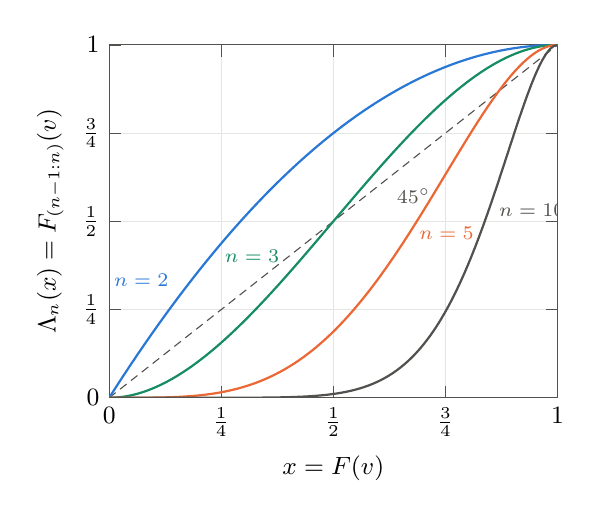
\begin{tikzpicture}
\begin{axis}[
  width=0.6\textwidth, height=0.5\textwidth,
  xlabel={$x=F(v)$}, ylabel={$\Lambda_n(x)=F_{(n-1:n)}(v)$},
  xmin=0, xmax=1, ymin=0, ymax=1, domain=0:1, samples=121,
  xtick={0,0.25,0.5,0.75,1}, xticklabels={$0$,$\frac14$,$\frac12$,$\frac34$,$1$},
  ytick={0,0.25,0.5,0.75,1}, yticklabels={$0$,$\frac14$,$\frac12$,$\frac34$,$1$},
  grid=major, grid style={c15gray!15}, axis line style={c15gray}, tick style={c15gray},
  label style={font=\small}, tick label style={font=\small}]
\addplot[c15gray, densely dashed] {x} node[pos=0.62, below right, font=\scriptsize] {$45^{\circ}$};
\addplot[c15blue, thick] {2*x - x^2} node[pos=0.22, above left, font=\scriptsize] {$n=2$};
\addplot[c15aqua!80!black, thick] {3*x^2 - 2*x^3} node[pos=0.38, above left, font=\scriptsize] {$n=3$};
\addplot[c15orange, thick] {5*x^4 - 4*x^5} node[pos=0.58, right, font=\scriptsize] {$n=5$};
\addplot[c15gray, thick] {10*x^9 - 9*x^10} node[pos=0.70, right, font=\scriptsize] {$n=10$};
\end{axis}
\end{tikzpicture}
\caption{The map $\Lambda_n$ from the value distribution to the distribution of the transaction price,
$\Lambda_n(x)=nx^{n-1}-(n-1)x^n$. Each curve is strictly increasing, so the price distribution determines $F$. The
curves are flat near $x=0$ when $n$ is large, which is why the lower tail of $F$ is hard to recover from prices.}
\label{fig:15-lambda}
\end{figure}

\begin{theorem}[{\citealp[Theorem~1]{AtheyHaile2002}}]\label{thm:15-ah1}
In the SIPV model of the ascending or second-price auction:
\begin{enumerate}[label=(\roman*)]
\item $F$ is identified from the distribution of the transaction price, and more generally from the distribution of
any single order statistic $B^{(k:n)}$ with known $n$.
\item The model is testable if either (a) more than one bid per auction is observed, or (b) transaction prices are
observed from auctions with exogenously varying numbers of bidders.
\end{enumerate}
\end{theorem}

\begin{proof}
(i) Bids equal values, so $B^{(k:n)}=V^{(k:n)}$ and the observed CDF of $B^{(k:n)}$ in $n$-bidder auctions,
$G_B^{(k:n)}$, equals $F_{(k:n)}$. By \eqref{eq:15-Lambda},
\[
G_B^{(k:n)}(v)=\Lambda_{k:n}\big(F(v)\big)\quad\text{for all }v .
\]
Since $\Lambda_{k:n}$ is strictly increasing and continuous, it has a continuous inverse, and
\[
F(v)=\Lambda_{k:n}^{-1}\big(G_B^{(k:n)}(v)\big).
\]
The transaction price is $B^{(n-1:n)}$, the case $k=n-1$. Under SIPV the marginal $F$ determines
$F_{\bm V}=\prod_iF(v_i)$.

(ii) Suppose the distributions of two order statistics $B^{(k:n)}$ and $B^{(k':n')}$ are observed, with
$(k,n)\neq(k',n')$. Under the model each implies a value distribution, and the two must coincide:
\[
\Lambda_{k:n}^{-1}\big(G_B^{(k:n)}(v)\big)=\Lambda_{k':n'}^{-1}\big(G_B^{(k':n')}(v)\big)\quad\text{for all }v .
\]
Pairs of distributions that violate this equality are easy to construct, so the restriction is refutable. Case (a)
supplies two order statistics from the same auctions. In case (b), exogenous participation guarantees that the same
$F$ governs auctions with different $n$.
\end{proof}

The result rests on independence and symmetry, and both can fail in ways the test detects. Independence is
testable even with a single bid per auction, because \eqref{eq:15-Lambda} dictates exactly how the price
distribution must move with $n$. The restriction fails in natural examples with asymmetric or strictly affiliated
values \citep[footnote~20]{AtheyHaile2002}. The test also has power against the button model itself. In free-form
oral auctions recorded bids often understate willingness to pay. Comparing estimates from low-ranked bids with
estimates from high-ranked bids then measures how far bidders fall short of their values
\citep[footnote~19]{AtheyHaile2002}.

\begin{example}[Two and three bidders]\label{ex:15-asc-n2}
With $n=2$, the price is the lower of two values and $\Lambda_2(x)=2x-x^2$. Let $H_2$ denote the CDF of the price in
two-bidder auctions. Then
\[
1-H_2(v)=1-2F(v)+F(v)^2=\big(1-F(v)\big)^2,
\qquad\text{so}\qquad
F(v)=1-\sqrt{1-H_2(v)} .
\]
The survival function of the minimum is the square of the survival function of one value. With $n=3$,
$\Lambda_3(x)=3x^2-2x^3$, and $F(v)$ is the unique root in $[0,1]$ of the cubic $3x^2-2x^3=H_3(v)$. Since
$\Lambda_3(\frac12)=\frac34-\frac14=\frac12$, the median price in three-bidder auctions equals the median value. The
second-highest of three draws is their median, and the median of three draws has the same median as each draw.
\end{example}

\casehead{Estimation}
The identification argument is constructive. Following \citet[Section~4.2]{AtheyHaile2007}, let
\[
\hat H_n(v)=\frac{1}{T_n}\sum_{t=1}^T\indic\big(n_t=n,\ P_t\le v\big)
\]
be the empirical CDF of prices in $n$-bidder auctions. Its population counterpart is the price CDF
$H_n(v)=\Lambda_n\big(F(v)\big)$. The estimator is $\hat F(v)=\Lambda_n^{-1}\big(\hat H_n(v)\big)$.
It is computed at each $v$ by bisection, which is fast because $\Lambda_n$ is monotone. Uniform
consistency of $\hat H_n$ carries over to $\hat F$ through the continuity of $\Lambda_n^{-1}$.

The delta method (\cref{thm:A-delta}) gives the precision of $\hat F$. At a point $v$ with $H_n(v)\in(0,1)$, the
empirical CDF satisfies
\[
\sqrt{T_n}\big(\hat H_n(v)-H_n(v)\big)\xrightarrow{d}N\Big(0,\ H_n(v)\big(1-H_n(v)\big)\Big).
\]
The inverse function rule gives the derivative of the transformation,
\[
\frac{d\Lambda_n^{-1}(y)}{dy}\bigg|_{y=H_n(v)}=\frac{1}{\Lambda_n'\big(\Lambda_n^{-1}(H_n(v))\big)}=\frac{1}{\Lambda_n'\big(F(v)\big)} .
\]
Therefore
\begin{equation}\label{eq:15-asc-var}
\sqrt{T_n}\big(\hat F(v)-F(v)\big)\xrightarrow{d}N\left(0,\ \frac{H_n(v)\big(1-H_n(v)\big)}{\Lambda_n'\big(F(v)\big)^2}\right),
\qquad \Lambda_n'(x)=n(n-1)x^{n-2}(1-x).
\end{equation}

The formula shows where prices are informative. In the lower tail, write $x=F(v)$ and let $x\to0$. Then
$H_n\approx nx^{n-1}$ and $\Lambda_n'(x)\approx n(n-1)x^{n-2}$, so the asymptotic variance in \eqref{eq:15-asc-var}
behaves like
\[
\frac{nx^{n-1}}{n^2(n-1)^2x^{2n-4}}=\frac{x^{3-n}}{n(n-1)^2}.
\]
It vanishes with $x$ when $n=2$, stays at $\frac{1}{12}$ when $n=3$, and explodes when $n\ge4$. A low value sets the
price only if $n-1$ values are low, an event of probability of order $x^{n-1}$, so prices carry little information
about the lower tail. The upper tail is also poorly estimated. Expanding around $x=1$ gives
$1-\Lambda_n(x)\approx\frac{n(n-1)}{2}(1-x)^2$ and $\Lambda_n'(x)\approx n(n-1)(1-x)$, so the asymptotic variance tends
to $\frac{1}{2n(n-1)}$. The estimator from all $n$ bids has asymptotic variance $\frac{x(1-x)}{n}$ per auction, which
vanishes at both ends. With $n=2$ the ratio of the two variances is $\frac{2-x}{2(1-x)}$, equal to one in the lower
tail and unbounded in the upper tail. The price never reveals the winner's value.

\Cref{fig:15-asc-sim} illustrates these properties on simulated data. Panel (a) shows that 500 transaction prices
from four-bidder auctions recover $F$ well. Panel (b) shows that the delta-method formula tracks the bootstrap
standard error closely. Compare it with the benchmark in which all bids are observed. At the median value the
price-only standard error is 24 percent larger, and at $v=0.5$, where $F=0.08$, it is more than four times larger
(our calculation from the simulation).

\begin{figure}[htbp]
\centering
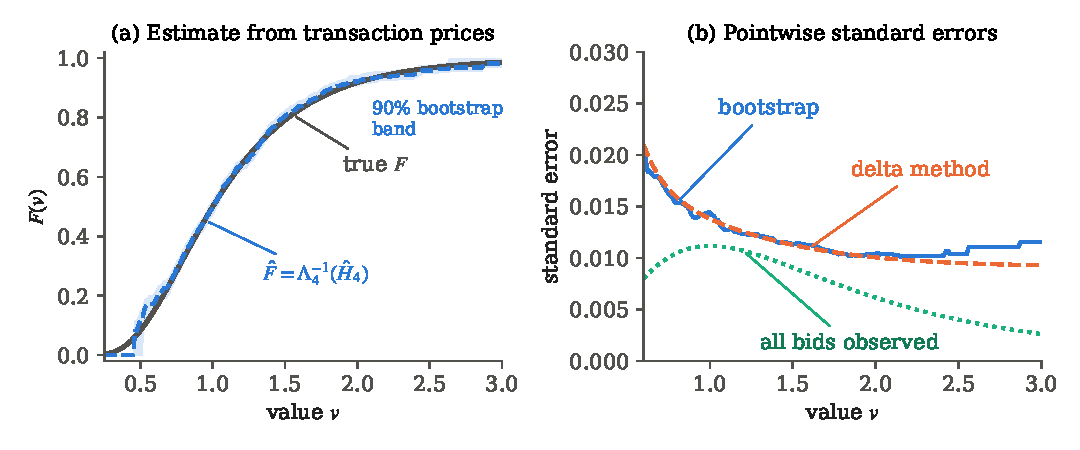
\includegraphics[width=\textwidth]{figures/ch15/asc_inversion.pdf}
\caption{Price-only inversion in simulated button auctions. Our simulation: $T=500$ auctions with $n=4$ bidders,
values lognormal with $\mu=0$ and $\sigma=\frac12$, seed 15201. Panel (a): true $F$, the estimate
$\hat F=\Lambda_4^{-1}(\hat H_4)$, and a pointwise 90 percent band from 500 bootstrap samples of whole auctions.
Panel (b): bootstrap standard error, the delta-method formula \eqref{eq:15-asc-var}, and the standard error of the
empirical CDF if all $4T$ values were observed. Panel (b) starts at $v=0.6$ because few prices fall below that
level.}\label{fig:15-asc-sim}
\end{figure}

Exogenous variation in $n$ yields one estimator $\Lambda_n^{-1}(\hat H_n)$ for each value of $n$ in the data. If
losing bids also follow the button model, each further order statistic yields another estimator through
$\Lambda_{k:n}^{-1}$. An efficient estimator would take an optimally weighted average of these estimators and impose
monotonicity of the estimated CDF \citep[Section~4.2]{AtheyHaile2007}. The differences among them are the basis of
the specification tests in \cref{thm:15-ah1}(ii).

\subsection{Asymmetric independent private values: competing risks}\label{sec:15-asym-ipv}

Independence alone suffices for identification from a single bid, provided we also observe who won. The argument
borrows from the statistics of \emph{competing risks}. A system fails as soon as one of its components fails, and
we observe the failure time and the component that failed. Up to a change of sign, this is the same as observing the
highest bid and the identity of the highest bidder \citep[footnote~21]{AtheyHaile2002}.

\begin{theorem}[{\citealp[Theorem~2]{AtheyHaile2002}}]\label{thm:15-ah2}
In the asymmetric IPV model, assume that each $F_i$ is continuous and that the support of $F_i$ is the same for all
$i$. Each $F_i$ is identified if either
\begin{enumerate}[label=(\alph*)]
\item the transaction price $B^{(n-1:n)}$ and the identity of the winner are observed, or
\item in a second-price auction, the highest bid $B^{(n:n)}$ and the identity of the winner are observed.
\end{enumerate}
Given (a) or (b), the model is testable in either of two cases.
\begin{enumerate}[label=(\roman*)]
\item Participation is exogenous, and each bidder faces at least two different sets of opponents.
\item The auction is second price, and both (a) and (b) hold.
\end{enumerate}
\end{theorem}

Independence is maintained in the theorem. What is relaxed relative to \cref{thm:15-ah1} is symmetry. We prove part
(b) for any $n$, part (a) for $n=2$, and then show the structure of part (a) for $n=3$. The general case of part (a)
is due to \citet[Theorem~1 and Section~4]{Meilijson1981}, and part (b) follows from results collected by
\citet[Theorem~7.3.1]{PrakasaRao1992}.

\begin{proof}[Proof of part (b)]
Let $\bar u$ be the upper end of the common support. For each bidder $i$ define the observable sub-distribution
\[
\tilde G_i(t)=\Pr\big(B^{(n:n)}\le t,\ I=i\big)=\int_{-\infty}^t f_i(x)\prod_{j\neq i}F_j(x)\,dx ,
\]
since bidder $i$ wins with bid $x$ when her value is $x$ and every rival's value is below $x$. The CDF of the highest
bid is $H(t)=\prod_jF_j(t)=\sum_i\tilde G_i(t)$, also observable. Differentiating $\tilde G_i$,
\[
\tilde g_i(t)=f_i(t)\prod_{j\neq i}F_j(t)=H(t)\,\frac{f_i(t)}{F_i(t)} .
\]
So the reverse hazard rate of $V_i$ equals the observable ratio $\frac{\tilde g_i(t)}{H(t)}$. Since
$\frac{f_i}{F_i}=\frac{d}{dt}\ln F_i$ and $\ln F_i(\bar u)=0$, integrating from $t$ to $\bar u$ gives
\[
F_i(t)=\exp\left(-\int_t^{\bar u}\frac{\tilde g_i(x)}{H(x)}\,dx\right).
\]
The right side is a functional of the distribution of observables.
\end{proof}

\begin{proof}[Proof of part (a) for $n=2$]
With two bidders the price is the lower value and the winner is the bidder with the higher value. For the event that
bidder 2 wins at a price of at most $t$,
\[
\tilde G_2(t)=\Pr\big(V_1\le t,\ V_1<V_2\big)=\int_{-\infty}^tf_1(x)\big(1-F_2(x)\big)\,dx .
\]
The price exceeds $t$ only if both values do, so its CDF $H$ satisfies $1-H(t)=\big(1-F_1(t)\big)\big(1-F_2(t)\big)$.
Dividing the density of $\tilde G_2$ by $1-H$ gives
\[
\frac{\tilde g_2(t)}{1-H(t)}=\frac{f_1(t)\big(1-F_2(t)\big)}{\big(1-F_1(t)\big)\big(1-F_2(t)\big)}=\frac{f_1(t)}{1-F_1(t)},
\]
the hazard rate of $V_1$. Integrating the hazard from the bottom of the support gives
$F_1(t)=1-\exp\big(-\int_{-\infty}^t\frac{\tilde g_2(x)}{1-H(x)}\,dx\big)$. The same steps with the roles reversed identify
$F_2$.
\end{proof}

With $n=3$ the argument of \citet[Section~4.1]{AtheyHaile2007} shows the structure of the general case. Let $\underline
u$ be the lower end of the support. Bidder 3 wins at a price of at most $t$ in two disjoint cases. Either both rivals
are below $t$ and bidder 3 is above $t$, or bidder 3 is below $t$ and above both rivals:
\begin{align*}
\tilde G_3(t)&=\Pr\big(V_1\le t,\ V_2\le t,\ V_3\ge t\big)+\Pr\big(V_1\le V_3,\ V_2\le V_3,\ V_3\le t\big)\\
&=F_1(t)F_2(t)\big(1-F_3(t)\big)+\int_{\underline u}^tF_1(x)F_2(x)\,dF_3(x).
\end{align*}
Integration by parts gives $\int_{\underline u}^tF_1F_2\,dF_3=F_1(t)F_2(t)F_3(t)-\int_{\underline u}^t(F_1F_2)'F_3\,dx$.
Substituting and writing $F_1(t)F_2(t)=\int_{\underline u}^t(F_1F_2)'\,dx$,
\[
\tilde G_3(t)=\int_{\underline u}^t\big(F_1(x)F_2(x)\big)'\big(1-F_3(x)\big)\,dx .
\]
Differentiating and rearranging, $(F_1F_2)'=\frac{\tilde g_3}{1-F_3}$. Integrating and taking logarithms,
\[
\ln F_1(t)+\ln F_2(t)=\ln\int_{\underline u}^t\frac{\tilde g_3(x)}{1-F_3(x)}\,dx\equiv R_3(t),
\]
and cyclically $\ln F_1+\ln F_3=R_2$ and $\ln F_2+\ln F_3=R_1$. The coefficient matrix of this system in
$(\ln F_1,\ln F_2,\ln F_3)$ has rows $(1,1,0)$, $(1,0,1)$ and $(0,1,1)$, and its determinant is $-2$. If the right
sides were known, the system would give, for example, $\ln F_1=\frac12(R_3+R_2-R_1)$. The right sides themselves
depend on the unknown distributions through $1-F_j$, so the system is a fixed-point problem.
\citet{Meilijson1981} shows that it has a unique solution.

Testability follows the logic of \cref{thm:15-ah1}. With exogenous participation, each set of opponents that bidder
$i$ faces delivers its own version of $F_i$, and the versions must agree. In a second-price auction with both (a)
and (b), the two constructions above must deliver the same $F_i$.

\casehead{Estimation}
The structure suggests a likelihood \citep[equation~(4.7)]{AtheyHaile2007}. Bidder $i$ wins at price $p$ when
some rival $j$ has value exactly $p$, every other rival $k$ has a value below $p$, and $V_i$ exceeds $p$. The
density of this event is $\big(1-F_i(p)\big)\sum_{j\neq i}f_j(p)\prod_{k\neq i,j}F_k(p)$, and the likelihood of a
sample of prices $p_t$ and winners $I_t$ is
\[
\mathcal L=\prod_{t=1}^T\big(1-F_{I_t}(p_t)\big)\sum_{j\neq I_t}f_j(p_t)\prod_{k\neq I_t,j}F_k(p_t).
\]
Parametric or semi-nonparametric maximum likelihood can be applied to it. \citet{BrendstrupPaarsch2006} develop a
semi-nonparametric estimator of this kind. Nonparametric estimators from the competing-risks literature, such as
the Kaplan-Meier estimator, are natural alternatives. \citet[Section~3.3.1]{AtheyHaile2007} make this suggestion for
the closely related problem of Dutch auctions with asymmetric bidders.

\subsection{Covariates}\label{sec:15-covariates}

Real auctions sell heterogeneous objects, and bidders differ in observable ways. Covariates are usually a nuisance,
but they can also be a source of identification.

\begin{theorem}[{\citealp[Theorem~3]{AtheyHaile2002}}]\label{thm:15-ah3}
Let private values be $V_i=g_i(A_i,Z)$, where each $g_i$ is an unknown function strictly increasing in $A_i$. Each
$F_{A_i}$ is continuous with the same support for all $i$. The auction covariates $Z$ and the transaction price are
observed, together with the identity of the winner if bidders are asymmetric.
\begin{enumerate}[label=(\roman*)]
\item If $A_1,\dots,A_n$ are independent conditional on $Z$, each conditional distribution $F_{V_i}(\cdot\mid z)$ is
identified. In the asymmetric case we assume in addition that, for each $z$, the conditional value
distributions $F_{V_i}(\cdot\mid z)$ are continuous and share a common support.
\item If $g_i(A_i,Z)=A_i+g_0(Z)$ for all $i$, and $A_1,\dots,A_n$ are mutually independent and independent of $Z$, then
the distribution of $\bm A$ and the function $g_0$ are identified up to location.
\item The symmetric models in (i) and (ii) are testable with more than one bid per auction, or with transaction
prices from auctions with exogenously varying numbers of bidders.
\end{enumerate}
\end{theorem}

\begin{proof}
(i) Fix $Z=z$. Values are independent given $z$, so \cref{thm:15-ah1} (symmetric case) or \cref{thm:15-ah2}
(asymmetric case) applies conditional on $z$. \Cref{thm:15-ah2} needs a common support of the value distributions,
which is why (i) imposes it on the $F_{V_i}(\cdot\mid z)$ directly.

(ii) Consider the symmetric case. Given $Z=z$ the price is $A^{(n-1:n)}+g_0(z)$, so its conditional CDF is
\[
H_n(b\mid z)=\Pr\big(A^{(n-1:n)}\le b-g_0(z)\big)=F_{A,(n-1:n)}\big(b-g_0(z)\big),
\]
where $F_{A,(n-1:n)}$ is the CDF of the second-highest of the $A_i$. Let $q_\tau(z)$ be the $\tau$-quantile of the
price given $z$, and $a_\tau$ the $\tau$-quantile of $A^{(n-1:n)}$. Then $q_\tau(z)=g_0(z)+a_\tau$, so
\[
g_0(z)-g_0(z')=q_\tau(z)-q_\tau(z')\quad\text{for all }z,z' ,
\]
and $g_0$ is identified up to an additive constant. A location normalization, such as $g_0(z_0)=0$ at a reference
point, fixes the constant. The price net of $g_0(Z)$ is then $A^{(n-1:n)}$, whose distribution identifies $F_A$ by
\cref{thm:15-ah1}. The asymmetric case uses \cref{thm:15-ah2} instead.

(iii) Two order statistics, or two values of $n$, give two versions of $F_{V}(\cdot\mid z)$ in (i), or of $F_A$ in
(ii), and these must coincide.
\end{proof}

\citet{AtheyHaile2002} state the support condition for the $A_i$. That suffices in (ii), where every value is
$A_i+g_0(z)$ and the supports shift together. In the asymmetric case of (i) it does not suffice, because
different functions $g_i$ need not preserve a common support. Let $A_1$ and $A_2$ be independent and uniform on
$[0,1]$, with $g_1(a)=a$ and $g_2(a)=a+2$. In an ascending auction bidder 2 always wins, at the price $A_1$.
Replacing $g_2(a)$ by $a+3$ leaves the joint distribution of the price and the winner unchanged, yet it changes
$F_{V_2}$.

Part (ii) is the basis of \emph{homogenization}. Write the price in auction $t$ as
\[
P_t=g_0(Z_t)+A_t^{(n_t-1:n_t)}=\kappa(n_t)+g_0(Z_t)+\varepsilon_t,
\qquad \kappa(n)=\E\big[A^{(n-1:n)}\big],\quad \E[\varepsilon_t\mid Z_t,n_t]=0 .
\]
A regression of prices on covariates and on indicators for $n$ estimates $g_0$, parametrically or flexibly. The
homogenized prices $P_t-\hat g_0(Z_t)$ are then treated as prices of identical objects, and the inversion of
\cref{sec:15-price-only} estimates $F_A$ \citep[equation~(6.6)]{AtheyHaile2007}. The first step matters for
inference. Suppose $\hat g_0$ converges at the parametric rate $T^{-\frac12}$. At a point $v$, the empirical CDF of
the homogenized prices then differs from its infeasible counterpart by approximately $f_{A,(n-1:n)}(v)$, the
density of $A^{(n-1:n)}$, times the average estimation error of $\hat g_0(Z_t)$. This term has the same order
$T^{-\frac12}$ as the sampling error of the empirical CDF itself.
Standard errors for $\hat F_A$ must therefore account for the first step, for example by bootstrapping both
steps together. The first step is asymptotically negligible only for second-step estimators that converge more
slowly, such as a kernel estimator of the density of $A$, under the usual smoothness conditions.
The function $g_0$ is often of interest in its own right, since it measures how observables shift valuations. In
first-price auctions the same idea requires that equilibrium bidding preserve the additive structure, which
\cref{lem:15-separability} establishes (\cref{sec:15-uh-sep} applies it to bids). Here it is immediate because
bids equal values. Alternatives to homogenization are
kernel smoothing over covariates, which \citet{HaileTamer2003} apply to ascending auctions, and flexible
mixtures for the conditional price distribution \citep[Section~6.1.1]{AtheyHaile2007}.

Bidder covariates do more. They can identify models with arbitrary correlation among values, which the next
subsection shows are not identified from bids alone. The idea comes from the Roy model, in which a worker chooses
the sector that offers the highest wage, and we observe only that wage and the chosen sector
\citep[footnote~29]{AtheyHaile2002}. Suppose $V_i=g_i(W_i)+A_i$ and suppose for a moment that the maximum value is
observed. Then
\[
\Pr\big(V^{(n:n)}\le u\mid\bm w\big)=\Pr\big(A_i\le u-g_i(w_i)\ \forall i\big)=F_{\bm A}\big(u-g_1(w_1),\dots,u-g_n(w_n)\big).
\]
The joint distribution of values is observed only along its diagonal. Variation in the indices $g_i(w_i)$, however,
moves the point at which $F_{\bm A}$ is evaluated over all of $\R^n$. When $g_j(w_j)$ is very negative for every
$j\neq i$, bidder $i$ has the highest value with probability close to one, and variation in $w_i$ traces out
$g_i$ \citep[Section~6.2.1]{AtheyHaile2007}. The following result shows that the same logic works for any single
order statistic, including the transaction price of an ascending auction.

\begin{theorem}[{\citealp[Theorem~6.1]{AtheyHaile2007}}]\label{thm:15-ah5}
Assume the following.
\begin{enumerate}[label=(\roman*)]
\item $V_i=g_i(W_i)+A_i$ for $i=1,\dots,n$.
\item $F_{\bm A}$ has support $\R^n$ and a continuously differentiable density $f_{\bm A}$.
\item The vector $(A_1,\dots,A_n)$ is independent of $(W_1,\dots,W_n)$.
\item The support of $\big(g_1(W_1),\dots,g_n(W_n)\big)$ is $\R^n$.
\item Each $g_i$ is continuously differentiable, with $g_i(w)\to\infty$ as $w\to\infty$ and $g_i(w)\to-\infty$ as
$w\to-\infty$.
\end{enumerate}
Then $F_{\bm A}$ and each $g_i$ are identified up to location from the distribution of $\big(V^{(j:n)},\bm W\big)$, for
any single $j\in\{1,\dots,n\}$.
\end{theorem}

The theorem allows arbitrary dependence among the $A_i$ and arbitrary asymmetry. It is a slight modification of
Theorem~5 of \citet{AtheyHaile2002} that corrects a minor error in its proof \citep[footnote~55]{AtheyHaile2007}. The
survey states condition (iii) pairwise, as independence of each $A_i$ and each $W_j$, while its text assumes that
the vector of the $A_i$ is independent of all covariates. The proof needs the vector form. Under pairwise
independence alone the correlation among the $A_i$ could vary with $\bm W$ while every marginal stays fixed. We
give a direct proof for scalar covariates.

\begin{proof}
Write $\bm z(u,\bm w)=\big(u-g_1(w_1),\dots,u-g_n(w_n)\big)$. For a set of bidders $\mathcal T\subseteq\{1,\dots,n\}$
define
\[
\bar F^{\mathcal T}(\bm a)=\Pr\big(A_i>a_i\ \forall i\in\mathcal T,\ A_k\le a_k\ \forall k\notin\mathcal T\big),
\]
so that $\bar F^{\emptyset}=F_{\bm A}$.

\emph{Step 1.} The $j$-th lowest value is at most $u$ exactly when at least $j$ values are at most $u$. Equivalently,
the set $\mathcal T$ of bidders with $V_i>u$ has at most $n-j$ members. Since $V_i>u$ if and only if
$A_i>u-g_i(w_i)$, and since by (iii) the distribution of $\bm A$ given $\bm W=\bm w$ is $F_{\bm A}$,
\[
\Pr\big(V^{(j:n)}\le u\mid\bm w\big)=\sum_{\mathcal T:\,|\mathcal T|\le n-j}\bar F^{\mathcal T}\big(\bm z(u,\bm w)\big).
\]

\emph{Step 2.} Write $\bar F^{\mathcal T}$ as an integral of $f_{\bm A}$ over $a_i>z_i$ for $i\in\mathcal T$ and
$a_k\le z_k$ for $k\notin\mathcal T$. Differentiating once in each $z_k$ gives a plus sign for upper limits and a
minus sign for lower limits, so
\[
\frac{\partial^n\bar F^{\mathcal T}(\bm z)}{\partial z_1\cdots\partial z_n}=(-1)^{|\mathcal T|}f_{\bm A}(\bm z).
\]

\emph{Step 3.} Since $\frac{\partial z_k}{\partial w_k}=-g_k'(w_k)$, the chain rule gives
\[
\frac{\partial^n}{\partial w_1\cdots\partial w_n}\bar F^{\mathcal T}\big(\bm z(u,\bm w)\big)
=(-1)^{|\mathcal T|}f_{\bm A}(\bm z)\prod_{k=1}^n\big(-g_k'(w_k)\big).
\]

\emph{Step 4.} Summing over the sets in Step~1, there are $\binom{n}{m}$ sets of size $m$. The identity
$\sum_{m=0}^{K}(-1)^m\binom nm=(-1)^K\binom{n-1}{K}$ follows from Pascal's rule by telescoping. With $K=n-j$ and the
case $\mathcal T=\emptyset$ of Step~3,
\[
\frac{\partial^n}{\partial w_1\cdots\partial w_n}\Pr\big(V^{(j:n)}\le u\mid\bm w\big)
=(-1)^{n-j}\binom{n-1}{n-j}\,\frac{\partial^n}{\partial w_1\cdots\partial w_n}F_{\bm A}\big(\bm z(u,\bm w)\big).
\]

\emph{Step 5.} Integrate each $\tilde w_k$ from $w_k$ to $\infty$. As $\tilde w_k\to\infty$, $g_k(\tilde w_k)\to\infty$, so
$z_k\to-\infty$ and $F_{\bm A}\to0$. Repeated use of the fundamental theorem of calculus gives
\[
\int_{w_1}^{\infty}\!\!\cdots\int_{w_n}^{\infty}\frac{\partial^nF_{\bm A}\big(\bm z(u,\tilde{\bm w})\big)}{\partial\tilde w_1\cdots\partial\tilde w_n}\,
d\tilde w_n\cdots d\tilde w_1=(-1)^nF_{\bm A}\big(\bm z(u,\bm w)\big).
\]
Combining with Step~4,
\[
F_{\bm A}\big(\bm z(u,\bm w)\big)=\frac{(-1)^j}{\binom{n-1}{n-j}}\int_{w_1}^{\infty}\!\!\cdots\int_{w_n}^{\infty}
\frac{\partial^n\Pr\big(V^{(j:n)}\le u\mid\tilde{\bm w}\big)}{\partial\tilde w_1\cdots\partial\tilde w_n}\,d\tilde w_n\cdots d\tilde w_1 ,
\]
which is equation (6.17) of \citet{AtheyHaile2007}. The right side is observable.

\emph{Step 6.} Let $w_k\to-\infty$ for every $k\neq i$. Then $z_k\to\infty$ and the left side tends to
$F_{A_i}\big(u-g_i(w_i)\big)$. This function of $(u,w_i)$ is known. Since $F_{A_i}$ is strictly increasing, any two
points with the same value satisfy $u-g_i(w_i)=u'-g_i(w_i')$, so $g_i(w_i)-g_i(w_i')=u-u'$. Hence $g_i$ is identified
up to an additive constant. With the $g_i$ known, condition (iv) lets us choose $u$ and $\bm w$ with
$\bm z(u,\bm w)$ equal to any point $\bm a\in\R^n$, which identifies $F_{\bm A}(\bm a)$.
\end{proof}

Two order statistics give two expressions for $F_{\bm A}$, and their equality is a testable restriction
\citep[Theorem~5(ii)]{AtheyHaile2002}. The result needs large support: bidder covariates must push every bidder's
value far above and far below the others'. Estimators that exploit it had not been developed when
\citet[Section~6.2.1]{AtheyHaile2007} wrote.

\subsection{Correlated values: what incomplete bids cannot reveal}\label{sec:15-nonid}

The positive results above lean on independence or on rich covariates. Without either, the picture changes.

\begin{theorem}[{\citealp[Theorem~4]{AtheyHaile2002}}]\label{thm:15-ah4}
In the symmetric private values model:
\begin{enumerate}[label=(\roman*)]
\item $F_{\bm V}$ is not identified from the vector of bids in an ascending auction.
\item In a second-price auction, $F_{\bm V}$ is not identified unless all bids are observed.
\end{enumerate}
\end{theorem}

\begin{proof}
We construct two exchangeable distributions that generate the same observables. Suppose $f_{\bm V}$ is positive on a
neighborhood of $[0,5]^n$. Let the $k$-th order statistic be the one that is not observed, where $k=n$ in an
ascending auction because the winner never exits. Fix $0<\varepsilon<\frac12$ and write $\mathcal Q(\bm c)$ for the
cube of half-width $\varepsilon$ centered at $\bm c$.

Start with $n=2$ and $k=2$, so only $\min(V_1,V_2)$ is observed. Let
\[
c(\bm v)=\indic_{\mathcal Q(1,3)}(\bm v)+\indic_{\mathcal Q(3,1)}(\bm v)-\indic_{\mathcal Q(1,2)}(\bm v)-\indic_{\mathcal Q(2,1)}(\bm v),
\]
and $\tilde f_{\bm V}=f_{\bm V}+\gamma c$ with $\gamma>0$ below the minimum of $f_{\bm V}$ on the four squares. Then
$\tilde f_{\bm V}\ge0$, and it integrates to one because the squares have equal areas. It is symmetric in $(v_1,v_2)$,
so it is exchangeable. On $\mathcal Q(1,2)$ and $\mathcal Q(1,3)$ the minimum is $v_1$, and the perturbation adds and
removes the same uniform mass for $v_1$ on $[1-\varepsilon,1+\varepsilon]$. The same holds on $\mathcal Q(2,1)$ and
$\mathcal Q(3,1)$ with the roles of the coordinates reversed. Hence the distribution of $\min(V_1,V_2)$ is unchanged.
The marginal density of $V_1$, however, gains $2\varepsilon\gamma$ on $[3-\varepsilon,3+\varepsilon]$ and loses
$2\varepsilon\gamma$ on $[2-\varepsilon,2+\varepsilon]$. Two different joint distributions, with different
marginals, generate the same observables.

For general $n$ and $k$, partition the bidders into one bidder $i$, a set of $k-1$ bidders and a set of $n-k$ bidders.
Consider the point at which the $k-1$ bidders have value 1, bidder $i$ has value 2, and the $n-k$ bidders have value
4. Shift mass $\gamma$ from the cube around this point to the cube around the point at which bidder $i$ has value 3
instead. Repeat for every such partition, which preserves exchangeability. Each shift moves only the $k$-th order statistic, from near 2
to near 3, while every other order statistic keeps the same local distribution. The joint distribution of the
observed order statistics is therefore unchanged \citep[proof of Theorem~4]{AtheyHaile2002}.
\end{proof}

\begin{figure}[htbp]
\centering
\begin{tikzpicture}[scale=0.92]
\def\e{0.3}
\fill[c15blue!7] (1-\e,5) -- (1-\e,1-\e) -- (5,1-\e) -- (5,1+\e) -- (1+\e,1+\e) -- (1+\e,5) -- cycle;
\draw[c15gray!60] (0,0) rectangle (5,5);
\draw[c15gray, densely dashed] (0,0) -- (5,5);
\draw[-{Stealth[length=2mm]}, c15gray] (0,0) -- (5.5,0) node[right] {$v_1$};
\draw[-{Stealth[length=2mm]}, c15gray] (0,0) -- (0,5.5) node[above] {$v_2$};
\foreach \x in {1,2,3,4,5} {\draw[c15gray] (\x,0) -- (\x,-0.08) node[below, font=\scriptsize] {$\x$};
  \draw[c15gray] (0,\x) -- (-0.08,\x) node[left, font=\scriptsize] {$\x$};}
\foreach \px/\py in {1/2,2/1} {\fill[c15orange!45] ({\px-\e},{\py-\e}) rectangle ({\px+\e},{\py+\e});}
\foreach \px/\py in {1/3,3/1} {\fill[c15blue!45] ({\px-\e},{\py-\e}) rectangle ({\px+\e},{\py+\e});}
\node[font=\scriptsize] at (1,2) {$-\gamma$};
\node[font=\scriptsize] at (2,1) {$-\gamma$};
\node[font=\scriptsize] at (1,3) {$+\gamma$};
\node[font=\scriptsize] at (3,1) {$+\gamma$};
\draw[-{Stealth[length=1.6mm]}, thick, c15gray] (1.42,2.25) -- (1.42,2.75);
\draw[-{Stealth[length=1.6mm]}, thick, c15gray] (2.25,1.42) -- (2.75,1.42);
\node[font=\scriptsize, align=left, anchor=west] at (2.0,4.3) {shaded strip:\\ $\min(v_1,v_2)\in[1-\varepsilon,1+\varepsilon]$};
\draw[c15gray, thin] (2.0,4.3) -- (1.25,4.0);
\end{tikzpicture}
\caption{The construction behind \cref{thm:15-ah4} for $n=2$. Mass $\gamma$ moves from the orange squares to the blue
squares, symmetrically about the diagonal. All four squares lie in the shaded strip, and within each pair the minimum
has the same distribution. The law of $\min(V_1,V_2)$, the only observable in a two-bidder ascending auction, is
therefore unchanged, while the marginal distribution of each value changes.}\label{fig:15-perturb}
\end{figure}

\Cref{fig:15-perturb} draws the construction. The intuition is a matter of dimension. Even under exchangeability,
$F_{\bm V}$ is an $n$-dimensional distribution, and identifying it from data of dimension $n-1$ or lower requires
additional restrictions \citep[Section~3.3.2]{AtheyHaile2007}. The result generalizes a classic finding of the
competing-risks literature, in which the joint distribution of risks is not identified from the distribution of the
first failure time alone \citep[footnote~26]{AtheyHaile2002}. Affiliation does not rescue identification, because a
small enough perturbation preserves strict affiliation \citep[footnote~27]{AtheyHaile2002}. The marginal $F$ itself
is not identified, so even the distribution of a single bidder's value is out of reach.

Taken together, \cref{thm:15-ah1,thm:15-ah2,thm:15-ah4,thm:15-ah5} describe a trade-off. One may relax the data,
observing only the transaction price, if values are independent. One may relax the model, allowing correlation,
if the data are richer: all bids, or bidder covariates with large support. One cannot relax both at once.
\citet{AradillasLopezGandhiQuint2013} study the case in between. With correlated private values and transaction
prices from auctions with exogenously varying numbers of bidders, $F_{\bm V}$ is not point identified. They show
that the reserve-price question does not need all of $F_{\bm V}$ \citep[pp.~88--89]{HortacsuPerrigne2021}. In an
ascending auction with reserve $r$ and seller value $v_0$, a sale occurs when $V^{(n:n)}\ge r$, at the price
$\max\{V^{(n-1:n)},r\}$. The seller's expected profit is therefore
\[
\pi(r)=\E\big[(V^{(n-1:n)}-v_0)\indic\{V^{(n-1:n)}\ge r\}\big]+(r-v_0)\Pr\big(V^{(n-1:n)}<r\le V^{(n:n)}\big),
\]
and the last probability equals $F_{(n-1:n)}(r)-F_{(n:n)}(r)$. Transaction prices identify $F_{(n-1:n)}$. Only the
distribution of the highest value at the single point $r$ is missing. It lies between $F_{(n-1:n)}(r)$ and, under
their assumptions, the value $\big[\Lambda_{n-1:n}^{-1}\big(F_{(n-1:n)}(r)\big)\big]^n$ that independence would imply.
For $r\ge v_0$ the profit falls in $F_{(n:n)}(r)$, so these limits bound $\pi(r)$. The bounds are wide.
Exogenous variation in $n$ tightens them, because the joint law of any $m<n$ values drawn at random must then
be the same in auctions of every size (p.~89, footnote 5). \Cref{sec:15-reserve-asc} reports their estimates for
timber sales.

\subsection{An incomplete model of ascending auctions}\label{sec:15-ht}

The button model is a stylized description of an English auction. In many oral auctions bidders call out prices
themselves and nontrivial minimum increments are common. A bidder may jump bid, or stay silent until the auction is
about to end \citep[Section~4.3]{AtheyHaile2007}. Bidders then fail to reveal their full willingness to
pay, and some never bid. Losing bids need not equal values, and the price need not equal the second-highest value.
\citet{HaileTamer2003} replace the button model by two weak behavioral assumptions.

\begin{assumption}[\citealp{HaileTamer2003}]\label{ass:15-ht}
Values are SIPV and the number of bidders $n$ is observed. Let $\Delta\ge0$ be the minimum bid increment.
\begin{enumerate}[label=(HT\arabic*),leftmargin=*]
\item Bidders do not bid more than they are willing to pay: $b_i\le v_i$ for every bidder.
\item Bidders do not allow an opponent to win at a price they are willing to beat: every losing bidder has
$v_i\le b^{(n:n)}+\Delta$, where $b^{(n:n)}$ is the winning bid.
\end{enumerate}
\end{assumption}

The assumptions allow the dominant-strategy behavior of the button model but do not require it. Bids need not be
monotone in values. The model is \emph{incomplete}: it restricts the relation between values and bids without fully
characterizing behavior. It cannot identify $F$, but it bounds it. Let $G_B^{(i:n)}$ be the CDF of the $i$-th lowest
bid in $n$-bidder auctions, and let $G_\Delta^{(n:n)}$ be the CDF of $B^{(n:n)}+\Delta$.

\begin{theorem}[{\citealp{HaileTamer2003} and \citealp[Theorem~4.3]{AtheyHaile2007}}]\label{thm:15-ht}
Under \cref{ass:15-ht}, $F^-(v)\le F(v)\le F^+(v)$ for all $v$, where
\[
F^+(v)=\min_{n}\ \min_{1\le i\le n}\ \Lambda_{i:n}^{-1}\big(G_B^{(i:n)}(v)\big),\qquad
F^-(v)=\max_{n}\ \Lambda_{n-1:n}^{-1}\big(G_\Delta^{(n:n)}(v)\big).
\]
\end{theorem}

\begin{proof}
\emph{Upper bound.} By HT1, $b_i\le v_i$ for every $i$. The value $v^{(i:n)}$ is at least as large as $i$ of the
values, and the bids of those $i$ bidders are no larger than their values. So at least $i$ bids are at most
$v^{(i:n)}$, which means $b^{(i:n)}\le v^{(i:n)}$. Hence the event $\{V^{(i:n)}\le v\}$ implies $\{B^{(i:n)}\le v\}$,
and
\[
G_B^{(i:n)}(v)\ge F_{(i:n)}(v)=\Lambda_{i:n}\big(F(v)\big).
\]
Applying the increasing function $\Lambda_{i:n}^{-1}$ to both sides gives $\Lambda_{i:n}^{-1}\big(G_B^{(i:n)}(v)\big)\ge F(v)$.
This holds for every $i$ and every $n$, so it holds for the minimum.

\emph{Lower bound.} By HT2, all $n-1$ losing bidders have values at most $b^{(n:n)}+\Delta$. At least $n-1$ values are
therefore below this level, so $v^{(n-1:n)}\le b^{(n:n)}+\Delta$. The event $\{B^{(n:n)}+\Delta\le v\}$ implies
$\{V^{(n-1:n)}\le v\}$, and
\[
G_\Delta^{(n:n)}(v)\le F_{(n-1:n)}(v)=\Lambda_{n-1:n}\big(F(v)\big).
\]
Applying $\Lambda_{n-1:n}^{-1}$ gives $\Lambda_{n-1:n}^{-1}\big(G_\Delta^{(n:n)}(v)\big)\le F(v)$ for every $n$, hence for the
maximum.
\end{proof}

Several features of the bounds matter in practice. If only the transaction price is recorded, the upper bound uses
$i=n$ alone. The number of bidders must be observed, which holds when bidders must register or qualify, as in the
timber auctions studied by \citet{HaileTamer2003}. If the data satisfy the button model and $\Delta\to0$, the bounds
collapse to $F$. Conversely, imposing the button model when it is false need not produce an estimate inside the
bounds, even in large samples. Imposing false structure to obtain point identification differs from selecting a
point inside the bounds of a correct incomplete model \citep[Section~4.3.1]{AtheyHaile2007}.

Estimation replaces each CDF by its empirical counterpart. Each component $\Lambda_{i:n}^{-1}(\hat G_B^{(i:n)})$ is
consistent and asymptotically normal, but the minimum and maximum have non-normal limits, and inference uses the
bootstrap. The minimum of several consistent estimators tends to select one with a downward sampling error, and the
maximum one with an upward error. The estimated bounds are therefore too narrow in finite samples and may even cross.
\citet{HaileTamer2003} replace the minimum and maximum by smooth weighted averages that approach them as the sample
grows.

\casehead{Bounds on the optimal reserve price}
The seller's main policy instrument in the SIPV model is the reserve price. Let $v_0$ be the seller's value. By
\cref{cor:14-optimal-reserve}, the optimal reserve $r^*$ solves $r^*-\frac{1-F(r^*)}{f(r^*)}=v_0$. Bounds on $F$ place
no restriction on its derivative at a point, so plugging $F^+$ or $F^-$ into this equation does not bound $r^*$. A
detour through an objective function works. Define
\[
\pi(r)=(r-v_0)\big(1-F(r)\big).
\]
Then $\pi'(r)=\big(1-F(r)\big)-(r-v_0)f(r)=-f(r)\big[\psi(r)-v_0\big]$, where $\psi$ is the virtual valuation
\eqref{eq:14-psi}. So $\pi$ has the same maximizer as the seller's expected profit, although it is not that profit when
$n>1$ \citep[footnote~34]{AtheyHaile2007}. For $r\ge v_0$, the bounds on $F$ imply
\[
\pi_1(r)\equiv(r-v_0)\big(1-F^+(r)\big)\le\pi(r)\le\pi_2(r)\equiv(r-v_0)\big(1-F^-(r)\big).
\]
Let $r_1^*$ maximize $\pi_1$, let $\pi_1^*=\pi_1(r_1^*)$, and define
\[
r^-=\sup\{r<r_1^*:\pi_2(r)\le\pi_1^*\},\qquad r^+=\inf\{r>r_1^*:\pi_2(r)\le\pi_1^*\}.
\]

\begin{proposition}[{\citealp{HaileTamer2003} and \citealp[Theorem~4.4]{AtheyHaile2007}}]\label{prop:15-ht-reserve}
Suppose $\pi$ is continuously differentiable and strictly quasi-concave. Then $r^*\in[r^-,r^+]$. Given the bounds
$F^+$ and $F^-$, the bounds $r^-$ and $r^+$ are sharp.
\end{proposition}

\begin{proof}[Proof of the inclusion]
We treat the nontrivial case $r^-<r_1^*<r^+$ and assume $\pi_2$ is continuous.
\citet[Section~4.3.2]{AtheyHaile2007} discuss the degenerate cases, in which $r^-=r^+=r_1^*$. The true objective
satisfies
$\pi(r^*)\ge\pi(r_1^*)\ge\pi_1(r_1^*)=\pi_1^*$. Suppose $r^*<r^-$. Then $r^-$ lies strictly between $r^*$ and
$r_1^*$, and strict quasi-concavity gives
\[
\pi(r^-)>\min\{\pi(r^*),\pi(r_1^*)\}\ge\pi_1^* .
\]
By continuity $\pi_2(r^-)\le\pi_1^*$, so $\pi(r^-)\le\pi_2(r^-)\le\pi_1^*$, a contradiction. The case $r^*>r^+$ is
symmetric.
\end{proof}

\Cref{fig:15-ht} applies the bounds to simulated auctions. Losing bidders stop between 80 and 100 percent of their
values, and the price may fall up to one increment below the second-highest value. The bounds contain the true
$F$ over most of the range where the data are informative. The naive estimator that treats losing bids as values
lies above the upper bound, because it ignores the fact that bidders stopped short. The implied interval for the
optimal reserve is $[0.53,1.04]$, and it contains the true optimum $0.77$ (our simulation).

\begin{figure}[htbp]
\centering
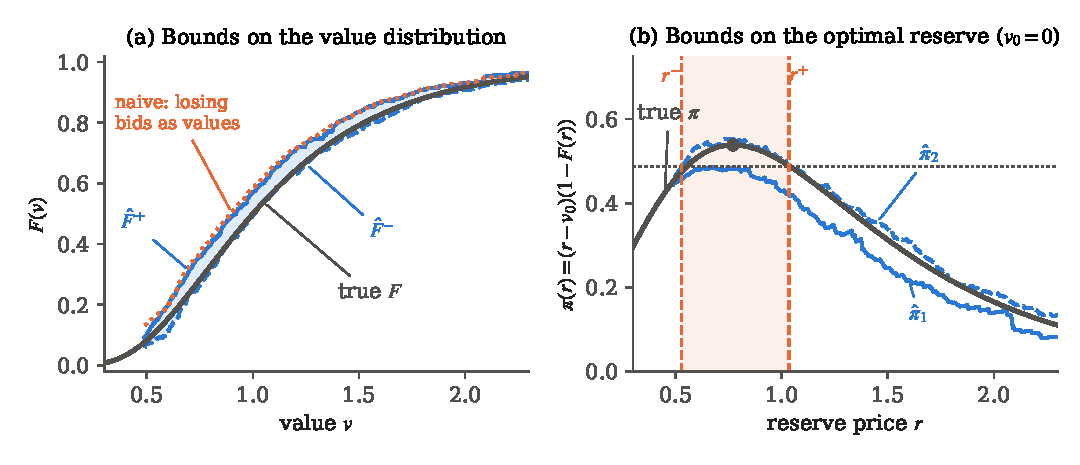
\includegraphics[width=\textwidth]{figures/ch15/ht_bounds.pdf}
\caption{Bounds from an incomplete model of ascending auctions. Our simulation: 500 auctions with $n=3$ and 500 with
$n=5$, values lognormal with $\mu=0$ and $\sigma=\frac12$, increment $\Delta=0.05$, seed 15202. Losing bidders record
bids equal to their values times a uniform draw on $[0.8,1]$. The winning bid lies between the second-highest value
minus $\Delta$ and that value, and is at least every losing bid. Panel (a): $\hat F^+$, $\hat F^-$, the true $F$ and
the naive estimate that inverts the highest losing bid as if it were the second-highest value. An order statistic is
used at $v$ only if at least 1 percent of its observations lie on each side of $v$, and curves are drawn where both
bounds are informative. Panel (b): $\hat\pi_1$, $\hat\pi_2$ and the true $\pi$ for $v_0=0$, with the interval
$[r^-,r^+]$ shaded and the true optimum marked by a dot.}\label{fig:15-ht}
\end{figure}

The approach extends in principle to asymmetric and affiliated private values, but the bounds are then likely to be
wide. Bounds on realized values reveal little about their correlation structure, and many policy questions need that
structure \citep[Section~4.3.3]{AtheyHaile2007}.

\subsection{Binding reserve prices}\label{sec:15-reserve-asc}

A reserve price $r$ inside the support of values, with $F(r)\in(0,1)$, separates potential bidders from actual
bidders. In this subsection $N$ is the number of potential bidders and $n_t$ the number who participate. With private
values a bidder participates exactly when her value is at least $r$. Under independence, the participants' values
are therefore i.i.d.\ draws from the truncated distribution
\begin{equation}\label{eq:15-truncated}
F(v\mid r)=\frac{F(v)-F(r)}{1-F(r)},\qquad v\ge r
\end{equation}
\citep[equation~(6.18)]{AtheyHaile2007}. In an ascending auction with $n_t\ge2$ participants, the price is the
second-highest of $n_t$ draws from $F(\cdot\mid r)$. With $n_t=1$ the price equals $r$.

\begin{proposition}[{\citealp[Corollary~3]{AtheyHaile2002} and \citealp[Corollary~6.1 and Theorem~6.3]{AtheyHaile2007}}]\label{prop:15-reserve-ident}
Consider the SIPV model of a first-price, second-price or ascending auction with reserve price $r$ and
$F(r)\in(0,1)$.
\begin{enumerate}[label=(\roman*)]
\item Consider a second-price or ascending auction, or a first-price auction whose participants learn their number
before they bid. If one bid from each auction and the number of participants are observed, $F(\cdot\mid r)$ is
identified on $[r,\infty)$.
\item The model is testable if two bids from each auction are observed, or if one bid is observed in auctions with
different numbers of participants.
\item If $N$ is fixed and the number of participants is observed, $N$ and $F(r)$ are identified. Combined with (i),
$F(v)$ is then identified for every $v\ge r$.
\item Consider a first-price auction whose bidders know $N$ but not the number of participants when they bid. If $N$
is fixed and one bid from each auction and the number of participants are observed, then $N$, $F(r)$ and $F(v)$
for every $v\ge r$ are identified.
\end{enumerate}
\end{proposition}

\begin{proof}
Parts (i) and (ii) apply \cref{thm:15-ah1} to the truncated distribution \eqref{eq:15-truncated}, conditioning on
the number of participants. In second-price and ascending auctions this is valid because bidding one's value is
a dominant strategy. In a first-price auction whose participants know their number $n_t$, each participant faces
$n_t-1$ rivals with values drawn from $F(\cdot\mid r)$, and the inversion of \cref{sec:15-gpv} applies to that
distribution. In the setting of (iv), condition (C2) of \cref{thm:15-gpv-reserve} makes participants' bids
i.i.d.\ given their number, with a distribution that does not depend on that number. Two bids per auction, or one
bid at different numbers of participants, then give two versions of that distribution, and these must coincide.
For part (iii), each potential bidder participates independently with probability $1-F(r)$, so the
number of participants is binomial with parameters $N$ and $1-F(r)$. Its distribution determines both parameters. Exchangeability gives a
convenient formula. The probability that a given bidder stays out is the same for every bidder. It therefore
equals the expected fraction of bidders who stay out:
\[
F(r)=\Pr(\text{bidder 1 does not bid})=\frac{\E[N-n_t]}{N}=\sum_{k=1}^{N}\frac{k}{N}\Pr\big(n_t=N-k\big),
\]
which is equation (6.19) of \citet{AtheyHaile2007}. Finally, \eqref{eq:15-truncated} gives
$F(v)=F(r)+\big(1-F(r)\big)F(v\mid r)$ for $v\ge r$.

For part (iv), a participant who bids $b\ge r$ wins when each of her $N-1$ potential rivals either stays out or bids
less. Her win probability therefore depends on $N$ and $F(r)$, and the inversion conditional on $n_t$ misstates her
first-order condition. Take $N=2$, values uniform on $[0,1]$ and $r=\frac12$, for example. The equilibrium bid is
$\beta(v)=\frac{v}{2}+\frac{1}{8v}$. Applied to two-participant auctions, the inversion of \cref{sec:15-gpv} maps
the bid of a bidder with value $\frac34$ to about $0.611$. The correct inversion \eqref{eq:15-gpv-reserve} uses
$N$ and $F(r)$, which part (iii) identifies. Given their number, participants' bids are i.i.d., so the observed
bid and that number identify the distribution of a participant's bid. When the observed bid is the highest, this
step is the root formula of \cref{prop:15-winbid}. \Cref{thm:15-gpv-reserve} then gives $F(v)$ for $v\ge r$.
\end{proof}

\citet[Corollary~3]{AtheyHaile2002} state (i) for first-price auctions as well, without saying what bidders know
about participation. The information structure matters. Part (iv) adopts that of \citet{GuerrePerrigneVuong2000},
in which bidders do not see who participates, and \cref{sec:15-gpv-reserve} develops it.

The sample analog of the formula that completes part (iii), $\hat F(v)=\hat F(r)+\big(1-\hat F(r)\big)\hat F(v\mid r)$, is consistent. Below
the reserve the data are silent without parametric assumptions. Is the truncated distribution enough for the
reserve-price question? The next result says that it usually is.

\begin{proposition}[{\citealp[Theorem~6.2]{AtheyHaile2007}}]\label{prop:15-trunc-reserve}
For a univariate CDF $\Phi$, let $\pi(\tilde r;\Phi)=(\tilde r-v_0)\big(1-\Phi(\tilde r)\big)$ and let $p^*(\Phi)$ maximize
$\pi(\cdot;\Phi)$ over the support of $\Phi$. Suppose $\pi(\cdot;F)$ is continuously differentiable and strictly
quasi-concave, and write $F_{\mid r}=F(\cdot\mid r)$.
\begin{enumerate}[label=(\roman*)]
\item If $r<p^*(F)$, then $p^*(F_{\mid r})=p^*(F)$.
\item If $r\ge p^*(F)$, then $p^*(F_{\mid r})=r$.
\end{enumerate}
\end{proposition}

\begin{proof}
For $\tilde r\ge r$, \eqref{eq:15-truncated} gives $1-F(\tilde r\mid r)=\frac{1-F(\tilde r)}{1-F(r)}$, so
\[
\pi(\tilde r;F_{\mid r})=\frac{\pi(\tilde r;F)}{1-F(r)}\qquad\text{for all }\tilde r\ge r .
\]
On the support of $F_{\mid r}$ the two objectives differ by a positive multiplicative constant. If $r<p^*(F)$, the
unconstrained maximizer lies in $[r,\infty)$ and both objectives peak there. If $r\ge p^*(F)$, strict
quasi-concavity makes $\pi(\cdot;F)$ decreasing on $[r,\infty)$, so the truncated objective peaks at its lower end
$r$.
\end{proof}

In the SIPV model, the optimal reserve computed from participants alone, ignoring the selection created by the
reserve, is the true optimum unless the actual reserve already exceeds it. The data reveal when that happens,
because the estimated optimum then sits at the actual reserve. Variation in reserve prices across auctions does more.
Suppose reserves vary for reasons unrelated to values. Data from auctions with low reserves then reveal $F$ over a
longer range, and a reserve below the lower end of the support reveals all of $F$
\citep[Section~6.3.1]{AtheyHaile2007}. Reserve prices may instead respond to features of the object that bidders see
and the econometrician does not. A reserve then signals unobserved quality, and treating it as an exogenous
truncation point is a mistake. \citet{Roberts2013} builds an identification
strategy on this observation (\cref{sec:15-uh}). With a reserve price, the tests of private against common values
in \cref{sec:15-cv} remain available, because truncation at a common reserve preserves exchangeability
\citep[Corollary~4]{AtheyHaile2002}.

\casehead{Applications to timber sales}
Timber sales have been the main testing ground for these methods \citep[Section~2.1]{HortacsuPerrigne2021}.
The estimates agree on one point. Observed reserve prices are low relative to the optimum that most
models imply, and the gain from raising them depends on the information structure.

\citet{Paarsch1997} studies ascending timber auctions in British Columbia with a parametric model (pp.~87--88).
He treats the winning bid as the second-highest value, as in the button model. Bids are per species on
estimated volumes, while payments follow harvested volumes. He therefore rewrites each value in terms of an
average harvesting cost, and the winner is the bidder with the lowest cost. He specifies a parametric cost
function and a Weibull distribution. The estimated optimal reserve is then on average 3.4 to 4.2 times the
observed reserve, as the seller's value $v_0$ ranges from zero to the appraisal value of the timber.

\citet{HaileTamer2003} apply \cref{thm:15-ht,prop:15-ht-reserve} to Forest Service ascending auctions, with
data from Oregon (p.~88). They estimate bounds on the optimal reserve and on the implied gain. The increase in
the seller's profit ranges from little to 34 percent, depending on $v_0$. At high values of $v_0$ the optimal
reserve leaves more than 90 percent of tracts unsold. \citet{AradillasLopezGandhiQuint2013} use Oregon data
as well (p.~89). Their estimated bounds on the seller's profit are smaller than the profit computed under
independent values, and independence also overstates bidders' surplus. A reserve computed under independence
would be too high and could even lower the seller's profit. The authors note that an optimal reserve would
conflict with the Forest Service's mandate to sell about 85 percent of the tracts it offers. The mandate may
explain why observed reserves are low.

\citet{CoeyEtAl2017} exploit the asymmetry between loggers and mills of \cref{sec:15-als} to tighten
the bounds in California sales (p.~89). The lower bound on the optimal reserve is similar, while the upper bound
is 10 to 15 percent lower. \citet{CoeyLarsenSweeney2019} turn to the \emph{bidder exclusion effect}, the expected
fall in revenue when one of $N$ bidders is excluded at random (pp.~89--90). In an ascending auction with
private values the price is the second-highest value. Excluding a bidder lowers it to the third-highest value
exactly when the excluded bidder holds one of the two highest values, which happens with probability
$\frac{2}{N}$. The exclusion effect is therefore
\[
\frac{2}{N}\,\E\big[B^{(N-1:N)}-B^{(N-2:N)}\big],
\]
which needs two order statistics and the number of potential bidders. Under exogenous participation the
observed fall in revenue, $\E[B^{(N-1:N)}]-\E[B^{(N-2:N-1)}]$, must equal this effect. The difference is their
test statistic. A negative value is consistent with common values, and a zero value with private values, as
\citet{AtheyHaile2002} show \citep[footnote~6]{HortacsuPerrigne2021}. The same effect bounds the gain from an
optimal reserve without computing the reserve. By \cref{prop:14-bk}, an optimal reserve with $N-1$ bidders
raises less revenue than one more bidder without a reserve. In California sales the average revenue gain from
an optimal reserve is at most 13 percent. Exogenous participation is rejected, with positive selection, since
values tend to be higher in auctions with more participants (p.~90).

The first-price evidence points the same way. \citet{LiPerrigne2003} study French public timber sales by
first-price sealed bid with a secret reserve (p.~90). They model the reserve as random, equal to the seller's
value and independent of bidders' values, which are independent private values. The inversion of
\citet{GuerrePerrigneVuong2000}, developed in \cref{sec:15-gpv}, recovers the value distribution. The optimal announced reserve is on average 46 percent higher
than the secret one. It lowers the number of successful sales and raises total revenue only slightly, but it
doubles the seller's net profit.

\section{First-Price Auctions I: The Inversion Problem and Direct Methods}\label{sec:15-direct}

In first-price and Dutch auctions bidders shade their bids below their values, and the amount of shading depends on
the distribution of values. This section explains why that makes identification and estimation harder. It then
studies the direct route, maximum likelihood with its non-regularity and the simulated estimator of
\citet{LaffontOssardVuong1995}. It closes with a comparison of direct and indirect methods that motivates
\cref{sec:15-gpv}.

\subsection{Why first-price auctions are harder}\label{sec:15-fpa-hard}

In the SIPV model with reserve price $r$, a bidder with value $v\ge r$ bids (\cref{prop:14-rs})
\[
\beta(v)=v-\frac{\int_r^vF(t)^{n-1}\,dt}{F(v)^{n-1}} .
\]
Bids are observed and values are not. The bid function depends on the unknown $F$, the very object we want to
estimate \citep[Section~3.1]{AtheyHaile2007}. The distribution of bids $G(b)=F\big(\beta^{-1}(b)\big)$ therefore depends
on $F$ in two ways, directly through the distribution of values and indirectly through the equilibrium strategy
\citep[p.~529]{GuerrePerrigneVuong2000}. Even a closed-form bid function does not tell us how to recover $F$ from $G$.

The economics of shading also suggests the way out. A bidder trades off the probability of winning against the
surplus she earns when she wins. In a procurement auction a firm with cost $c$ chooses its bid $b$ to maximize
$(b-c)\Pr(\text{win}\mid b)$, exactly as an oligopolist chooses its price to maximize $(p-c)q(p)$. The win probability
plays the role of residual demand, and the first-order condition is an inverse elasticity rule
(see \eqref{eq:14-proc-foc} and \eqref{eq:14-proc-lerner}, and \cref{ch:theory}). In demand estimation we recover marginal costs from the
pricing first-order condition once demand is estimated (\cref{ch:diffprod,ch:blp}). In auctions we can recover values
from the bidding first-order condition once the distribution of rivals' bids is estimated. That is the indirect route
of \cref{sec:15-gpv}. The literature first took the direct route, which we study now.

\subsection{Maximum likelihood and its non-regularity*}\label{sec:15-ml}

Let $F(\cdot;\theta)$ be a parametric family with density $f(\cdot;\theta)$, $\theta\in\Theta\subset\R^K$, and suppose
for simplicity that there is no binding reserve price. Each bid is $B_{it}=\beta(V_{it};\theta)$ with $\beta$ strictly
increasing, so $G(b;\theta)=F\big(\beta^{-1}(b;\theta);\theta\big)$. Differentiating gives the bid density
\begin{equation}\label{eq:15-bid-density}
g(b;\theta)=\frac{f\big(\beta^{-1}(b;\theta);\theta\big)}{\beta'\big(\beta^{-1}(b;\theta);\theta\big)},
\qquad b\in\big[\beta(\underline v;\theta),\ \beta(\bar v(\theta);\theta)\big].
\end{equation}
The equilibrium differential equation \eqref{eq:14-rs-ode} gives $\beta'(v)=(n-1)\big(v-\beta(v)\big)\frac{f(v)}{F(v)}$.
Substituting it, with $\xi=\beta^{-1}(b;\theta)$,
\[
g(b;\theta)=\frac{F(\xi;\theta)}{(n-1)(\xi-b)} .
\]
The log-likelihood of all bids is $\ell(\theta)=\sum_t\sum_i\ln g(b_{it};\theta)$. If only the winning bid is
recorded, as in a Dutch auction, its CDF is $H(b;\theta)=F(\xi;\theta)^n$. Its density is
\[
h(b;\theta)=\frac{nF(\xi;\theta)^{n-1}f(\xi;\theta)}{\beta'(\xi;\theta)}=\frac{n}{n-1}\,\frac{F(\xi;\theta)^n}{\xi-b},
\]
which is equation (7) of \citet{LaffontOssardVuong1995}. With a binding reserve price the object goes unsold with
probability $F(r;\theta)^n$, and the likelihood takes a Tobit form with a mass point at $r$.

Maximum likelihood faces three obstacles. The first is computation. Each evaluation of $\ell(\theta)$ requires
$\beta^{-1}(b_{it};\theta)$ for every bid and every trial value of $\theta$. The bid function involves an integral and
has no closed form for most families. With asymmetric or affiliated values it solves a system of differential
equations, such as \eqref{eq:14-asym-foc}, which must be solved anew at each $\theta$. The second obstacle is regularity. The
upper end of the support of bids, $\beta(\bar v(\theta);\theta)$, depends on $\theta$. With only the winning bid, the
support is $[r,\E\max(Y,r)]$, where $Y$ is the largest of $n-1$ draws from $F$ \citep[p.~958]{LaffontOssardVuong1995}.
A parameter-dependent support violates the standard conditions for maximum likelihood (\cref{sec:A-mle-nonregular}).
The third obstacle is that practical applications were confined to families with closed-form bid functions and to
the SIPV model \citep[Section~3.2]{AtheyHaile2007}. \citet{DonaldPaarsch1993,DonaldPaarsch1996} study the
non-regular problem. They derive non-standard asymptotic distributions and propose estimators built on extreme order
statistics of the bids. The following example shows what goes wrong.

\begin{example}[Maximum likelihood with power-distributed values]\label{ex:15-power-mle}
Let $F(v;\theta)=\big(\frac{v}{\theta}\big)^\gamma$ on $[0,\theta]$ with $\gamma>0$ known and $\theta$ unknown, and let
there be no reserve price. As in \cref{ex:14-power}, rescaled to the support $[0,\theta]$,
\[
\int_0^v\Big(\frac{t}{\theta}\Big)^{\gamma(n-1)}dt=\frac{v}{\gamma(n-1)+1}\Big(\frac{v}{\theta}\Big)^{\gamma(n-1)}.
\]
Substituting into \eqref{eq:14-rs-bid} gives
\[
\beta(v)=v-\frac{v}{\gamma(n-1)+1}=c\,v,\qquad c=\frac{\gamma(n-1)}{\gamma(n-1)+1}.
\]
Bids $B=cV$ have CDF $G(b;\theta)=\big(\frac{b}{c\theta}\big)^\gamma$ on $[0,c\theta]$ and density
$g(b;\theta)=\gamma b^{\gamma-1}(c\theta)^{-\gamma}$. With $nT$ bids the likelihood is
\[
L(\theta)=\prod_{t=1}^T\prod_{i=1}^n\gamma\,b_{it}^{\gamma-1}(c\theta)^{-\gamma}\,\indic\big(b_{it}\le c\theta\big)
=\Big[\prod_{t,i}\gamma\,b_{it}^{\gamma-1}\Big](c\theta)^{-\gamma nT}\,\indic\Big(\theta\ge\frac{\max_{t,i}b_{it}}{c}\Big).
\]
The likelihood is zero for $\theta$ below $\frac{1}{c}\max_{t,i}b_{it}$ and strictly decreasing above it, so
\[
\hat\theta=\frac{1}{c}\max_{t,i}b_{it}.
\]
Its distribution follows from that of the maximum of $nT$ independent bids. For $0\le x\le T\theta$,
\[
\Pr\big(T(\theta-\hat\theta)>x\big)=\Pr\Big(\max_{t,i}B_{it}<c\Big(\theta-\frac{x}{T}\Big)\Big)
=\Big(1-\frac{x}{T\theta}\Big)^{\gamma nT}\longrightarrow e^{-\frac{\gamma n}{\theta}x}.
\]
So $T(\theta-\hat\theta)$ converges to an exponential distribution with mean $\frac{\theta}{\gamma n}$.
\end{example}

The estimator converges at rate $T$, faster than the usual $\sqrt T$, and its limit is not normal. The information
equality fails. The score of one bid is $\frac{\partial}{\partial\theta}\ln g(b;\theta)=-\frac{\gamma}{\theta}$, whose mean is not
zero, because the support moves with $\theta$. Standard errors from the inverse information matrix are therefore
invalid, and the nonparametric bootstrap fails for the sample maximum (\cref{prop:A-uniform-mle} and
\cref{sec:A-boot-fail}). The estimator also rests entirely on the largest bid, so a single error in the top bid moves
it. The same structure arises whenever the upper end of the bid support depends on the parameters, which is the rule
in first-price auctions.

\subsection{Laffont, Ossard and Vuong (1995): simulated nonlinear least squares*}\label{sec:15-lov}

\casehead{Question}
\citet{LaffontOssardVuong1995} ask how to estimate a general parametric distribution of private values from
first-price or Dutch auctions in which only the winning bid is observed. They want to allow heterogeneity across
auctions and an unknown number of bidders, and to avoid computing the equilibrium bid function. Earlier structural
work by \citet{Paarsch1992} had relied on families with closed-form bid functions
\citep[p.~954]{LaffontOssardVuong1995}.

\casehead{Model}
The model of their Section~2 is the SIPV first-price auction with reserve price $r_t$ and $n$ bidders. The
equilibrium bid (their eq.~(1)) is \eqref{eq:14-rs-bid}. The winning bid is $\beta\big(V_t^{(n:n)}\big)$ when
$V_t^{(n:n)}\ge r_t$ (eq.~(2)), and the optimal reserve solves $r^*=v_0+\frac{1-F(r^*)}{f(r^*)}$ (eq.~(4),
\cref{cor:14-optimal-reserve}). Heterogeneity enters through observed characteristics $z_t$:
\[
F_t(\cdot)=F(\cdot\mid z_t,\theta)\qquad\text{(their eq.~(5))}.
\]
The reserve price is not among the characteristics, which fits their application, where buyers and sellers have the
same information about market conditions \citep[p.~957]{LaffontOssardVuong1995}. To avoid a discontinuity when the
object is unsold, they set the winning bid equal to the reserve in that case (eq.~(6)):
\[
b^w_t=\beta_t\big(V_t^{(n:n)}\big)\,\indic\big(V_t^{(n:n)}\ge r_t\big)+r_t\,\indic\big(V_t^{(n:n)}<r_t\big).
\]
Its distribution has a mass $F_t(r_t)^n$ at $r_t$ and the density $h_t$ above $r_t$. Bidders draw new independent values
in every auction, which rules out the dynamic incentives of repeated auctions.

\casehead{Revenue equivalence as an estimation device}
The key step replaces the intractable bid function by a conditional expectation that is easy to simulate.

\begin{lemma}[\citealp{LaffontOssardVuong1995}, eq.~(12)]\label{lem:15-lov}
For $v\ge r$, $\ \beta(v)=\E\big[\max\{V^{(n-1:n)},r\}\mid V^{(n:n)}=v\big]$.
\end{lemma}

\begin{proof}
Given that the highest of $n$ i.i.d.\ values equals $v$, the other $n-1$ values are i.i.d.\ draws from $F$ truncated
to lie below $v$. Their maximum $V^{(n-1:n)}$ then has CDF $\big(\frac{F(y)}{F(v)}\big)^{n-1}$ on $y\le v$. This is the
distribution of the highest rival value $Y_1$ conditional on $Y_1<v$. Hence the right side equals
$\E\big[\max\{Y_1,r\}\mid Y_1<v\big]$, which is $\beta(v)$ by \eqref{eq:14-rs-condexp}.
\end{proof}

Applying the lemma at $v=V_t^{(n:n)}$ gives $b^w_t=\E\big[\max\{V_t^{(n-1:n)},r_t\}\mid V_t^{(n:n)}\big]$. The equality
also holds when the object is unsold, since both sides then equal $r_t$. Taking expectations conditional on
$x_t=(r_t,z_t)$ yields the moment that drives the estimator (their eqs.~(13)--(15)):
\begin{equation}\label{eq:15-lov-mean}
\begin{aligned}
m_t(\theta)\equiv\E\big[b^w_t\mid x_t\big]&=\E\big[\max\{V_t^{(n-1:n)},r_t\}\mid x_t\big]\\
&=\int\!\!\cdots\!\int\max\{u^{(n-1:n)},r_t\}\prod_{i=1}^nf_t(u_i)\,du_1\cdots du_n ,
\end{aligned}
\end{equation}
where $u^{(n-1:n)}$ is the second highest of $(u_1,\dots,u_n)$. This is revenue equivalence (\cref{prop:14-ret}). The
expected winning bid in a first-price auction equals the expected price in an English auction with the same reserve.
The right side needs no bid function: draw $n$ values, take the second highest, and compare it with the reserve.

\casehead{The simulator}
\citet{LaffontOssardVuong1995} use importance sampling. For each auction they choose a known density $g_t$ whose
support contains that of $f_t$. Before estimation they draw $S$ independent samples
$\bm u_t^s=(u^s_{1t},\dots,u^s_{nt})$, $s=1,\dots,S$, with each $u^s_{it}$ drawn from $g_t$. Their eqs.~(16)--(17) define
\[
X_{st}(\theta)=\max\big\{u^{s}_{(n-1:n)t},\,r_t\big\}\prod_{i=1}^n\frac{f_t(u^s_{it};\theta)}{g_t(u^s_{it})},
\qquad\bar X_t(\theta)=\frac1S\sum_{s=1}^SX_{st}(\theta).
\]
By construction $\E\big[\bar X_t(\theta)\mid x_t\big]=m_t(\theta)$. The draws do not depend on $\theta$ and are independent of
$b^w_t$ given $x_t$. Because $\theta$ enters only through the weights, outside the maximum, $\bar X_t(\theta)$ is twice
continuously differentiable in $\theta$ whenever $f$ is. Standard derivative-based optimization then applies, and the
asymptotic theory is simpler than for discontinuous simulators \citep[p.~961]{LaffontOssardVuong1995}.

\casehead{The bias of naive simulated least squares}
Nonlinear least squares with the exact mean would minimize $\frac1T\sum_t\big(b^w_t-m_t(\theta)\big)^2$. Replacing
$m_t$ by its simulator gives the naive criterion $Q_S(\theta)=\frac1T\sum_t\big(b^w_t-\bar X_t(\theta)\big)^2$ (their
eq.~(8)). To find its limit, decompose
\[
b^w_t-\bar X_t(\theta)=\big(b^w_t-m_t(\theta_0)\big)+\big(m_t(\theta_0)-m_t(\theta)\big)+\big(m_t(\theta)-\bar X_t(\theta)\big).
\]
Given $x_t$, the first and third terms have mean zero and are independent of each other, and the second is fixed.
Every cross product therefore has conditional mean zero, and
\[
\E\Big[\big(b^w_t-\bar X_t(\theta)\big)^2\,\Big|\,x_t\Big]=\sigma_0^2(x_t)+\big(m_t(\theta_0)-m_t(\theta)\big)^2+\frac1S\,\omega_t(\theta),
\]
where $\sigma_0^2(x_t)=\Var(b^w_t\mid x_t)$ and $\omega_t(\theta)=\Var\big(X_{st}(\theta)\mid x_t\big)$. The first term does not
depend on $\theta$ and the second is minimized at $\theta_0$. The third term, the simulation variance, does depend on
$\theta$. The naive estimator converges to the minimizer of the sum of the last two terms, which is generally not
$\theta_0$ (their eq.~(9)). It favors parameter values at which the simulator is less noisy, and it is inconsistent for
any fixed $S$.

The fix subtracts an unbiased estimate of the simulation variance. The sample variance of the draws, divided by
$S$, satisfies $\E\big[\frac{1}{S(S-1)}\sum_s\big(X_{st}(\theta)-\bar X_t(\theta)\big)^2\mid x_t\big]=\frac1S\omega_t(\theta)$. The
simulated nonlinear least squares (SNLS) criterion is therefore (their eq.~(11))
\begin{equation}\label{eq:15-snls}
Q_S^*(\theta)=\frac1T\sum_{t=1}^T\left[\big(b^w_t-\bar X_t(\theta)\big)^2-\frac{1}{S(S-1)}\sum_{s=1}^S\big(X_{st}(\theta)-\bar X_t(\theta)\big)^2\right].
\end{equation}
Each bracket has conditional mean $\sigma_0^2(x_t)+\big(m_t(\theta_0)-m_t(\theta)\big)^2$, the same as the criterion of exact
nonlinear least squares. \Cref{sec:A-snlls} treats the estimator in the general framework of simulation estimators.

\casehead{Asymptotic properties}
Their Proposition~1 shows that for any fixed $S$ the SNLS estimator $\hat\theta$ is strongly consistent as $T\to\infty$,
provided $\theta_0$ is identified from the first moment of the winning bid. The minimized criterion $Q_S^*(\hat\theta)$
consistently estimates the mean squared error of the model. Proposition~2 gives asymptotic normality. Let
$\mu_t=\frac{\partial m_t(\theta_0)}{\partial\theta}$ and $Y_{st}=\frac{\partial X_{st}(\theta_0)}{\partial\theta}$, and let $\omega_t$,
$\Omega_t$ and $C_t$ be the conditional variances of $X_{st}(\theta_0)$ and $Y_{st}$ and their conditional covariance. Then
$\Sigma^{-\frac12}\sqrt T(\hat\theta-\theta_0)\xrightarrow{d}N(0,I_K)$ with $\Sigma=A^{-1}BA^{-1}$ and
\begin{align*}
A&=\frac1T\sum_{t=1}^T\E\big[\mu_t\mu_t^\top\big],\\
B&=\frac1T\sum_{t=1}^T\E\left[\sigma_0^2(x_t)\mu_t\mu_t^\top+\frac1S\Big(\sigma_0^2(x_t)\Omega_t+\omega_t\mu_t\mu_t^\top\Big)
+\frac{1}{S(S-1)}\Big(\omega_t\Omega_t+C_tC_t^\top\Big)\right].
\end{align*}
The first term of $B$ alone gives the sandwich of exact nonlinear least squares. Simulation inflates the variance by a
term of order $\frac1S$, which vanishes as $S$ grows. Proposition~3 gives a heteroskedasticity-robust estimator of
$\Sigma$ that is consistent for fixed $S$ and requires neither $\sigma_0^2$ nor exact moments. Competing simulated
estimators, such as simulated maximum likelihood, are inconsistent for fixed $S$, because they simulate a nonlinear
function of an expectation \citep[p.~962]{LaffontOssardVuong1995}.

\casehead{An unknown number of bidders}
Bidders in a Dutch auction who never bid leave no trace, so $n$ may be unknown. Their Proposition~4 treats the true
$n_0$ as a parameter in a bounded set $\mathcal J$ of integers. For each $n\in\mathcal J$ compute $\hat\theta_n$ and
$Q^*_{S,n}(\hat\theta_n)$, and let $\hat n$ minimize the criterion over $\mathcal J$. Then $(\hat n,\hat\theta_{\hat n})$ converges almost
surely to $(n_0,\theta_0)$ for fixed $S$. Since $\hat n$ is discrete it converges faster than $\hat\theta$, and inference on
$\theta$ can proceed as if $n$ were known (their footnote~14). Identification of $n$ here rests on the parametric
family. Without $n$, the distribution of the winning bid does not even determine the distribution of a single bid
\citep[Section~3.3.1]{AtheyHaile2007}, as \cref{sec:15-gpv-winbid} shows.

\casehead{Extensions}
Three extensions broaden the method. First, if the econometrician observes only part $z_{1t}$ of the
characteristics $z_t=(z_{1t},z_{2t})$ that bidders see, a parametric model $h(z_2\mid r,z_1;\gamma)$ for the omitted part
can be integrated out. The simulator then draws $z_{2t}$ along with the values (their eqs.~(24)--(25)). Second, the
lemma lets us simulate $\beta(v)$ itself, by averaging $\max\{V^{(n-1:n)},r\}$ over draws given $V^{(n:n)}=v$. Higher
moments of the winning bid then become available for a method of simulated moments. Third, the moment
\eqref{eq:15-lov-mean} is the expected price of any standard auction with the same reserve, so the estimator applies
equally to English and second-price auctions \citep[p.~959]{LaffontOssardVuong1995}.

\casehead{Setting and data}
The application is a descending auction of greenhouse eggplants in Marmande, France. The sellers are farmers, and
the buyers are resale trading firms acting for retailers who placed orders at given prices before the market
opened. These prices are the buyers' valuations, which supports the private values assumption. In each round a
case of 15 to 350 kilos is offered. The seller announces a reserve price per kilo, and the clock starts high, for
example at fifteen francs when the usual price is about ten francs per kilo. The first buyer to stop the clock wins
and pays the current price \citep[p.~967]{LaffontOssardVuong1995}.

The data cover daily sales in the summer of 1990, from June to October. To avoid dynamic incentives within a day,
the authors keep only days on which a single case of a given size category was offered. Eggplants deteriorate
quickly, so one day's supply can be treated as independent of the previous day's trade. The sample has 81 auctions.
The winning bid averages 7.52 francs per kilo (standard deviation 2.21, range 2.00 to 11.98), and the reserve price
averages 6.43 (standard deviation 1.81, range 2.00 to 10.00). The correlation between winning bids and reserves is
0.962 \citep[Appendix~B]{LaffontOssardVuong1995}.

\begin{figure}[htbp]
\centering
\begin{subfigure}[t]{0.49\textwidth}
\centering
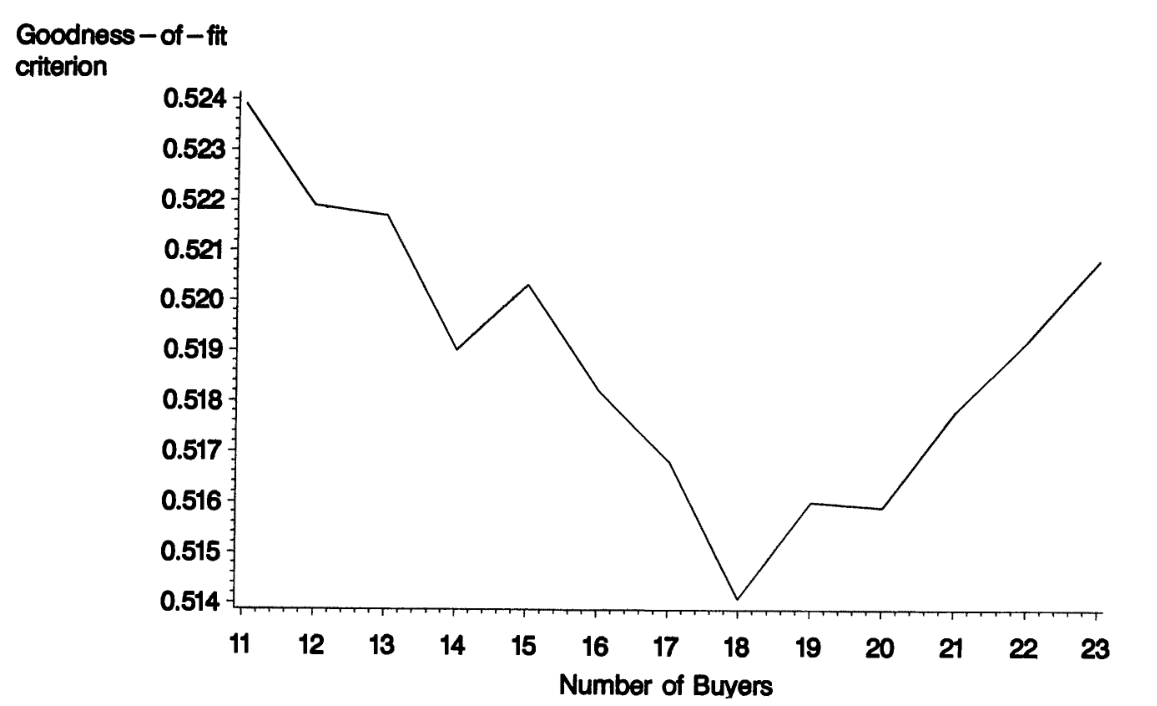
\includegraphics[width=\textwidth]{figures/ch15/lov1995_fig1.png}
\caption{Criterion $Q_S^*(\hat\theta_n)$ against the assumed number of buyers $n$.}\label{fig:15-lov-n}
\end{subfigure}\hfill
\begin{subfigure}[t]{0.49\textwidth}
\centering
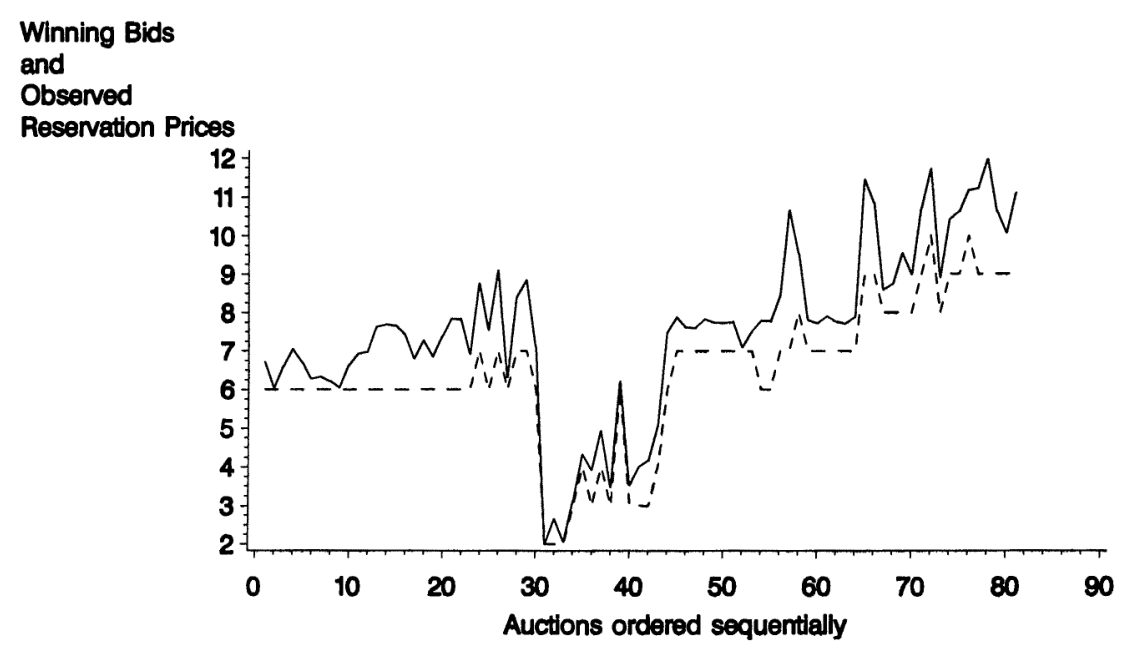
\includegraphics[width=\textwidth]{figures/ch15/lov1995_fig3.png}
\caption{Winning bids (solid) and reserve prices (dashed), auctions in chronological order.}\label{fig:15-lov-reserve}
\end{subfigure}
\caption{The Marmande eggplant auctions. Panel (a) selects the number of buyers by minimizing the simulated
criterion. Panel (b) shows that winning bids and reserve prices move together. Source: Laffont, Ossard and Vuong
(1995), Figures~1 and~3.}\label{fig:15-lov}
\end{figure}

\casehead{Specification}
Values are lognormal, a family without a closed-form bid function. The mean of log values is linear in six
characteristics (their eq.~(26)):
\[
\E\ln V_{it}=\mu_t=\theta_1+\theta_2\,\text{seller}_t+\theta_3\,\text{size1}_t+\theta_4\,\text{size2}_t+\theta_5\,\text{period}_t
+\theta_6\,\text{date}_t+\theta_7\,\text{supply}_t .
\]
The seller dummy is zero for the seller with the better reputation for quality (19 of the 81 lots come from the
other seller). The size dummies mark the middle category, 300 to 400 grams per eggplant (10 lots), and the largest
category, above 400 grams (34 lots). The period dummy is zero from the beginning of August until the first week of
September, when a large supply of substitute eggplants depresses prices, and one otherwise (68 lots). The date
variable records the time of the auction within 1990 divided by 100, so June 25 corresponds to 1.76. Supply is the
quantity of eggplants of all categories supplied at Marmande that day, in tons (mean 1.39).

The standard deviation $\sigma$ of $\ln V$ is not estimated. Retail prices for a given lot have a standard deviation of
about 5 percent of their mean. Setting $\frac{\text{sd}(V)}{\E(V)}=(e^{\sigma^2}-1)^{\frac12}=0.05$ gives $\sigma\approx0.05$
\citep[p.~969]{LaffontOssardVuong1995}. Their footnote~18 explains the choice. Reserve prices were low and every lot
was sold. Write $V=e^{\mu+\sigma U}$ with $U$ standard normal. Then $\E[b^w]=e^{\mu}\kappa(\sigma,\ln r-\mu)$, where
$\kappa(\sigma,a)=\E\big[\exp\big(\max\{\sigma U^{(n-1:n)},a\}\big)\big]$ for i.i.d.\ standard normal draws. As the reserve
becomes irrelevant, $\E[b^w]$ approaches $e^{\mu}\kappa(\sigma,-\infty)$, and the constant in $\mu$ cannot be separated
from $\sigma$. The estimator uses $S=20$ simulations per auction, and 30 give similar results. The importance density
for each auction is lognormal, centered at a preliminary consistent estimate and with standard deviation 0.05.

\casehead{Results}
The authors consider two hypotheses about the number of bidders. Eleven buyers attend regularly, but one buyer wins
almost half of the auctions and may act for several traders. They search over $n=11,\dots,23$, and the criterion is
smallest at $n=18$ (\cref{fig:15-lov-n}). The large buyer would then represent 8 traders, consistent with a market
share slightly below one half \citep[p.~970]{LaffontOssardVuong1995}. \Cref{tab:15-lov} reproduces their estimates for
$n=11$ and $n=18$.

\begin{table}[htbp]
\centering
\caption{Simulated nonlinear least squares estimates for the Marmande eggplant auctions}\label{tab:15-lov}
\begin{threeparttable}
\begin{tabular}{@{}lr@{\hspace{4pt}}rr@{\hspace{4pt}}r@{}}
\toprule
 & \multicolumn{2}{c}{$n=11$} & \multicolumn{2}{c}{$n=18$} \\
\cmidrule(lr){2-3}\cmidrule(l){4-5}
 & Estimate & ($t$) & Estimate & ($t$) \\
\midrule
Constant & 0.1297 & (0.02) & 0.0286 & (0.06) \\
Seller & $-0.0107$ & ($-0.17$) & $-0.0240$ & ($-0.51$) \\
Size 1 (300--400 g) & 0.2402 & (3.57) & 0.2402 & (4.39) \\
Size 2 (above 400 g) & 0.1373 & (1.39) & 0.1213 & (1.60) \\
Period & 1.2404 & (2.16) & 1.1998 & (2.90) \\
Date & 0.3115 & (3.04) & 0.3202 & (4.03) \\
Supply & $-0.0340$ & ($-0.59$) & $-0.0357$ & ($-0.81$) \\
\midrule
Criterion value $Q_S^*(\hat\theta)$ & \multicolumn{2}{c}{0.52395} & \multicolumn{2}{c}{0.51401} \\
Simulations per auction $S$ & \multicolumn{2}{c}{20} & \multicolumn{2}{c}{20} \\
Auctions $T$ & \multicolumn{2}{c}{81} & \multicolumn{2}{c}{81} \\
\bottomrule
\end{tabular}
\begin{tablenotes}
\footnotesize
\item \textit{Notes.} Reproduced from \citet[Table~I]{LaffontOssardVuong1995}. The coefficients are those of the mean of log
values, $\mu_t$ in their eq.~(26), with $\sigma=0.05$ imposed. Parentheses contain $t$-statistics computed from the robust
covariance estimator of their Proposition~3, not standard errors. Bids are in francs per kilo.
\end{tablenotes}
\end{threeparttable}
\end{table}

With a lognormal distribution and fixed $\sigma$, $\ln\E[V_t]=\mu_t+\frac{\sigma^2}{2}$, so each coefficient is
$\theta_k=\frac{1}{\E[V]}\frac{\partial\E[V]}{\partial x_k}$, a proportional effect on the expected value of the lot
\citep[p.~970]{LaffontOssardVuong1995}. With $n=18$, they read the size coefficients as midsize eggplants being worth
24 percent more than small ones and large ones 12 percent more. The size variables are dummies, so the exact
proportional effects are $e^{0.240}-1=27$ percent and $e^{0.121}-1=13$ percent (our calculation). This agrees with the conventional view that midsize eggplants are of the highest
quality. The seller coefficient is negative, so the seller with the better reputation commands higher values, but
the effect is small and insignificant. The period coefficient is large and significant. Values fall sharply during
the August glut, when \cref{fig:15-lov-reserve} shows winning bids dropping from about 7 francs to between 2 and 4
francs. The sample contains 13 lots with the period dummy equal to zero \citep[Appendix~B]{LaffontOssardVuong1995},
which matches the length of that run of low bids. Values also trend upward over the season (date). Local supply has no
significant effect, which the authors attribute to buyers serving several markets, with national supply movements
captured by the period and date variables. The fit is good: with $n=18$, $R^2=1-\frac{Q_S^*(\hat\theta)}{\widehat\Var(b^w)}=0.895$
\citep[p.~971]{LaffontOssardVuong1995}. The slope coefficients barely change between $n=11$ and $n=18$, while the
constant falls from 0.13 to 0.03. With more bidders the expected second-highest value is higher, so a lower level of
values fits the same winning bids.

\casehead{Assessment}
The paper made three contributions. It brought simulation-based estimation to structural auction models, with an
estimator that is consistent for a fixed number of simulations. It turned revenue equivalence into an estimation device. It
showed how to handle unobserved heterogeneity and an unknown number of bidders within the same framework. Its limits
are equally clear. The value distribution is parametric, and its dispersion was imposed from retail data rather than
estimated. The device relies on revenue equivalence, which fails with asymmetric bidders, affiliated values or risk
aversion. The dominant buyer is accommodated by inflating $n$, an assumption that holds only if that buyer bids for
each trader independently. Only the first moment of the winning bid is used.

\Cref{fig:15-lov-reserve} also raises a deeper issue. Winning bids and reserve prices move in tandem. If the reserve
were an exogenous truncation point, variation in reserves would change the fraction of lots sold, yet every lot was
sold. A more natural reading is that lots differ in ways that the seller and the buyers recognize and the
econometrician does not \citep[p.~7]{Roberts2013}. The authors anticipate the point in their conclusion. A seller may
set the reserve with better information than buyers, so that the reserve both truncates and shifts the distribution
of values \citep[p.~973]{LaffontOssardVuong1995}. \citet{Roberts2013} builds an identification strategy for
unobserved heterogeneity on exactly this co-movement (\cref{sec:15-uh}).

\subsection{From direct to indirect methods}\label{sec:15-direct-indirect}

Direct methods confront two burdens: solving the equilibrium for every trial parameter and a likelihood whose
support moves with the parameters. Simulated least squares removes the first burden with revenue equivalence and the
second by working with a smooth moment. Its reach is limited to models in which revenue equivalence holds. The
indirect approach of \citet{GuerrePerrigneVuong2000} removes both burdens in a different way. It estimates the
distribution of bids first and inverts the first-order condition \eqref{eq:14-foc-G} bid by bid, so no equilibrium is
ever computed. It also requires no parametric family (\cref{sec:15-gpv}).

Between the two lie hybrid two-step methods that specify a parametric first stage for bids conditional on
covariates, invert the first-order condition, and then work with the implied values
\citep{JofreBonetPesendorfer2003,AtheyLevinSeira2011}. They include covariates parsimoniously. A fully parametric
two-step method must keep the parametric families for bids and for values mutually consistent, because the
equilibrium bid function links them \citep{PerrigneVuong1999}. Making only one step parametric avoids that problem
\citep[Section~3.2]{AtheyHaile2007}. Theory also implies that bid distributions have compact support, so a parametric
first stage should impose an upper bound on bids \citep[footnote~19]{AtheyHaile2007}. \Cref{tab:15-direct-indirect}
summarizes the comparison.

\begin{table}[htbp]
\centering
\caption{Direct and indirect approaches to first-price auction data}\label{tab:15-direct-indirect}
\footnotesize
\begin{tabularx}{\textwidth}{@{}>{\raggedright\arraybackslash}p{2.0cm}>{\raggedright\arraybackslash}X>{\raggedright\arraybackslash}X>{\raggedright\arraybackslash}X>{\raggedright\arraybackslash}X@{}}
\toprule
 & Maximum likelihood & Simulated least squares & Two-step nonparametric & Two-step, parametric first stage \\
\midrule
Examples & \citet{Paarsch1992}, \citet{DonaldPaarsch1996} & \citet{LaffontOssardVuong1995} &
\citet{GuerrePerrigneVuong2000} & \citet{JofreBonetPesendorfer2003}, \citet{AtheyLevinSeira2011} \\
\addlinespace
Value distribution & parametric $F(\cdot;\theta)$ & parametric $F(\cdot;\theta)$ & unrestricted, smooth & implied by a
parametric bid distribution \\
\addlinespace
Equilibrium computation & solve and invert $\beta(\cdot;\theta)$ for every bid and every $\theta$ & none, since the
moment $\E\max\{V^{(n-1:n)},r\}$ is simulated & none, since the first-order condition is inverted & none, since the
first-order condition is inverted \\
\addlinespace
Regularity and rate & support depends on $\theta$, rate $T$ and non-normal limits & regular, $\sqrt T$ for fixed $S$,
variance excess of order $\frac1S$ & nonparametric rates slower than $\sqrt T$ & $\sqrt T$ for the bid parameters \\
\addlinespace
Data used & all bids or the winning bid & winning bid, $n$ may be unknown & all bids (the winning bid suffices under
SIPV) & all bids with covariates \\
\addlinespace
Asymmetry, affiliation, heterogeneity & a system of differential equations at every $\theta$ & excluded where revenue
equivalence fails, heterogeneity by integration & extends to all three (\cref{sec:15-apv,sec:15-uh}) & asymmetry,
dynamics, heterogeneity and entry \\
\addlinespace
Main drawback & computation, closed forms needed in practice & one moment, parametric family & dimensionality and
boundary trimming & consistency of bid and value families, support bounds \\
\bottomrule
\end{tabularx}
\end{table}

\section{First-Price Auctions II: The Guerre-Perrigne-Vuong Approach}\label{sec:15-gpv}

The direct methods of \cref{sec:15-direct} start from a parametric value distribution and solve for the equilibrium at every trial parameter. \citet{GuerrePerrigneVuong2000}, henceforth GPV, reversed the direction of the argument. They start from the distribution of observed bids and recover the value that rationalizes each bid. No equilibrium is ever computed, and no parametric family is assumed. This section develops their approach in full. It is the template for almost every structural method for first-price auctions that later sections use.

\casehead{The question} GPV pose three questions about the symmetric independent private values (SIPV) model of the first-price auction \citep[p.~526]{GuerrePerrigneVuong2000}. Does the model restrict the distribution of observable bids, so that it can be tested? Does identification of the value distribution require parametric assumptions? Can one estimate the value distribution without parametric assumptions and without solving for the equilibrium? Their answers are yes, no and yes. The model places two testable restrictions on bids. The value distribution is identified nonparametrically and constructively. A two-step kernel estimator recovers it, and no estimator can converge uniformly at a faster rate.

\casehead{Data} The method needs, for each auction $t=1,\dots,T$, all submitted bids $B_{1t},\dots,B_{n_tt}$, the number of bidders $n_t$, and the observed characteristics $Z_t$ of the object. These are the records of a sealed-bid first-price auction, such as a timber sale, a highway procurement or an offshore oil lease sale. GPV illustrate the method on simulated data, and we follow them in \cref{sec:15-gpv-mc}. Applications to field data appear in \cref{sec:15-apv,sec:15-uh,sec:15-als}.

\subsection{Setting and the inversion}\label{sec:15-gpv-insight}

We first state the model and the assumptions on the data-generating process, following GPV, Section 3.1. A single indivisible object is sold in each auction by a first-price sealed-bid auction. The highest bidder wins and pays her bid. Throughout \cref{sec:15-gpv-insight,sec:15-gpv-ident,sec:15-gpv-smooth,sec:15-gpv-estimator,sec:15-gpv-rates,sec:15-gpv-mc} the reserve price does not bind, so every potential bidder submits a bid and $n_t$ is the number of bidders who could have participated. \Cref{sec:15-gpv-reserve} treats a binding reserve price.

Let $Z_t\in\R^d$ collect the continuous characteristics of the object in auction $t$, and let $\mathcal I$ denote the set of possible numbers of bidders. The characteristics $Z_t$ are common knowledge among bidders. Their role is to absorb observed heterogeneity across auctions. They are not instruments.

\begin{assumption}[Sampling, GPV Assumption A1]\label{ass:15-gpv-sampling}
(i) Auctions are independent: the arrays $(Z_t,n_t,V_{1t},\dots,V_{n_tt})$, $t=1,2,\dots$, are independent across $t$, and the vectors $(Z_t,n_t)$ are identically distributed with density $f_{Zn}(z,n)$.
(ii) In each auction $t$, the values $V_{1t},\dots,V_{n_tt}$ are independent and identically distributed conditional on $(Z_t,n_t)$, with distribution $F(\cdot\mid Z_t,n_t)$ and density $f(\cdot\mid Z_t,n_t)$.
\end{assumption}

\begin{assumption}[Regularity, GPV Assumption A2]\label{ass:15-gpv-regularity}
The set $\mathcal I$ is a bounded subset of $\{2,3,\dots\}$, and the following hold.
(i) For each $n\in\mathcal I$, the support of $(V,Z)$ is $\{(v,z):z\in[\underline z,\bar z],\ v\in[\underline v(z),\bar v(z)]\}$ with $\underline z<\bar z$.
(ii) $f(v\mid z,n)\ge c_f>0$ on this support, and $f_{Zn}(z,n)\ge c_f>0$ on the support of $(Z,n)$.
(iii) For each $n\in\mathcal I$, $F(\cdot\mid\cdot,n)$ and $f_{Zn}(\cdot,n)$ have $R+1$ continuous bounded partial derivatives on their supports, with $R\ge 1$.
\end{assumption}

\Cref{ass:15-gpv-sampling} rules out dependence of values across auctions. GPV state part (i) for $(Z_t,n_t)$ only and invoke independence of values across auctions in the text, so we make it explicit. Such dependence would create dynamic incentives that the static equilibrium ignores. It allows the number of bidders to depend on the characteristics of the object. Part (iii) of \cref{ass:15-gpv-regularity} implies that the value density $f(\cdot\mid z,n)$ has $R$ bounded continuous derivatives. The integer $R$ measures smoothness and governs every rate of convergence below. The density is bounded away from zero, which keeps the bid density away from zero as well (\cref{prop:15-gpv-smooth}). GPV also assume, in the spirit of the theory, that $Z_t$ contains everything that bidders know about the object \citep[footnote 11]{GuerrePerrigneVuong2000}. Unobserved heterogeneity is the subject of \cref{sec:15-uh}.

\casehead{Equilibrium} Fix an auction with characteristics $z$ and $n$ bidders, and suppress $(z,n)$ when no confusion arises. Set the reserve price equal to $\underline v$. By \cref{prop:14-rs}, which gives the bid function of \citet{RileySamuelson1981}, the unique symmetric equilibrium bid is
\begin{equation}\label{eq:15-gpv-rs}
\beta(v)=v-\frac{1}{F(v)^{n-1}}\int_{\underline v}^{v}F(u)^{n-1}\,du,
\end{equation}
which is \eqref{eq:14-rs-bid} with $r=\underline v$ (GPV, eqs.~(1) and~(8)). It solves the differential equation
\begin{equation}\label{eq:15-gpv-ode}
1=\big(v-\beta(v)\big)(n-1)\frac{f(v)}{F(v)}\frac{1}{\beta'(v)}
\end{equation}
with the boundary condition $\beta(\underline v)=\underline v$ (GPV, eq.~(2)). This is \eqref{eq:14-rs-ode} divided by $\beta'(v)F(v)^{n-1}$. The bid function is strictly increasing on $[\underline v,\bar v]$.

\casehead{Why identification is not obvious} As \cref{sec:15-fpa-hard} explained, the bid distribution $G$ depends on $F$ in two ways. It depends on $F$ directly, because values are drawn from $F$. It also depends on $F$ through the strategy $\beta$, which by \eqref{eq:15-gpv-rs} is itself a functional of $F$. A direct method must untangle both channels for every trial value of $F$.

\casehead{The inversion} GPV observe that the first-order condition can be written so that the derivative $\beta'$, the distribution $F$ and the density $f$ disappear together. We derive the resulting formula step by step. Let $[\underline b,\bar b]=[\beta(\underline v),\beta(\bar v)]$ denote the support of bids, and note that $\underline b=\underline v$.

\emph{Step 1.} We express the bid distribution through $F$ and $\beta$. For $b\in[\underline b,\bar b]$, the strict monotonicity of $\beta$ gives
\[
G(b)=\Pr(B_i\le b)=\Pr\big(V_i\le\beta^{-1}(b)\big)=F\big(\beta^{-1}(b)\big).
\]

\emph{Step 2.} We differentiate. By the inverse function rule,
\[
g(b)=f\big(\beta^{-1}(b)\big)\frac{d\beta^{-1}(b)}{db}=\frac{f\big(\beta^{-1}(b)\big)}{\beta'\big(\beta^{-1}(b)\big)}.
\]

\emph{Step 3.} We take the ratio. Write $v=\beta^{-1}(b)$. Dividing the result of Step 2 by that of Step 1 gives
\[
\frac{g(b)}{G(b)}=\frac{1}{\beta'(v)}\,\frac{f(v)}{F(v)}.
\]

\emph{Step 4.} We substitute into the equilibrium condition. The right side of Step 3 is exactly the product that appears in \eqref{eq:15-gpv-ode}. Replacing it there and using $\beta(v)=b$ gives
\[
1=(v-b)(n-1)\frac{g(b)}{G(b)}.
\]

\emph{Step 5.} We solve for the value. Dividing by $(n-1)\frac{g(b)}{G(b)}$ and adding $b$ to both sides yields
\begin{equation}\label{eq:15-gpv-xi}
v=\xi(b;G,n)\equiv b+\frac{1}{n-1}\,\frac{G(b)}{g(b)}.
\end{equation}
This is GPV's equation~(3), and it coincides with \eqref{eq:14-foc-G}. With covariates, $G$ and $g$ are replaced by $G(\cdot\mid z,n)$ and $g(\cdot\mid z,n)$ (GPV, eq.~(9)).

Equation \eqref{eq:15-gpv-xi} expresses each value through the bid, the bid distribution, the bid density and the number of bidders. All four are observable or estimable. If bids are equilibrium bids, the value behind each bid must satisfy \eqref{eq:15-gpv-xi}. We call $\xi(\cdot;G,n)$ the \emph{inverse bid function}. In equilibrium it equals $\beta^{-1}$, and it has been obtained without solving \eqref{eq:15-gpv-ode}. We use the symbol $\xi$ for this object throughout the chapter, as GPV do (\cref{tab:15-notation}).

The same equation follows from the bidder's problem written in terms of bids, which is how \cref{sec:14-fpa-G} derived \eqref{eq:14-foc-G}. A bidder with value $v$ facing rivals whose bids are i.i.d.\ with distribution $G$ maximizes $(v-b)G(b)^{n-1}$. The first-order condition rearranges to \eqref{eq:15-gpv-xi}. The derivation above shows that the two routes agree. It also shows why the bid-based form is the right one for identification: it contains only objects that the data reveal.

\casehead{The markdown} The term $\frac{G(b)}{(n-1)g(b)}=v-b$ is the bidder's \emph{markdown}, the shading of the bid below the value. By \eqref{eq:14-markdown}, the relative markdown $\frac{v-b}{b}$ equals the inverse of the elasticity of the win probability $G(b)^{n-1}$ with respect to the bid. A bidder is a monopsonist facing the residual supply curve traced out by the highest rival bid. Equation \eqref{eq:15-gpv-xi} makes the oligopoly analogy of \cref{sec:15-fpa-hard} exact. The distribution of rival bids plays the role of the demand system, and the econometrician observes it directly.

\casehead{Credit and precursors} The idea first appeared in print in \citet{LaffontVuong1993}, who attribute it to an early draft of GPV \citep[Section 3.1]{AtheyHaile2007}. Similar formulas appear earlier in decision-theoretic models of bidding, starting with \citet{Friedman1956}. There each bidder optimizes against an exogenous distribution of rival bids, so the value distribution and the bid distribution need not be linked by $F=G\circ\beta$ \citep[footnote 3]{GuerrePerrigneVuong2000}. In \eqref{eq:15-gpv-xi} the link holds because bidders' beliefs about rival bids are correct in equilibrium.

\subsection{Identification and testable restrictions}\label{sec:15-gpv-ident}

We now state GPV's identification theorem. Let $\mathcal P$ denote the set of distributions on $\R_+$ that are absolutely continuous with an interval support. The support of a distribution in $\mathcal P$ is the closure of the set where its density is positive, so every member of $\mathcal P$ is strictly increasing on its support \citep[footnote 4]{GuerrePerrigneVuong2000}. Let $\mathbf G$ denote the joint distribution of the $n$ bids $(B_1,\dots,B_n)$ in an auction. As in GPV, we restrict attention to strictly increasing and differentiable equilibrium strategies.

\begin{theorem}[\citealp{GuerrePerrigneVuong2000}, Theorem 1]\label{thm:15-gpv-ident}
Let $n\ge 2$, and let $\mathbf G$ belong to $\mathcal P^n$ with support $[\underline b,\bar b]^n$. Consider a first-price sealed-bid auction with symmetric independent private values and a nonbinding reserve price. There exists a value distribution $F\in\mathcal P$ whose equilibrium bids have joint distribution $\mathbf G$ if and only if the following two conditions hold.
\begin{itemize}
\item[(C1)] $\mathbf G(b_1,\dots,b_n)=\prod_{i=1}^n G(b_i)$ for some distribution $G$.
\item[(C2)] The function $\xi(\cdot;G,n)$ defined in \eqref{eq:15-gpv-xi} is strictly increasing on $[\underline b,\bar b]$, and its inverse is differentiable on $[\underline v,\bar v]\equiv[\xi(\underline b;G,n),\xi(\bar b;G,n)]$.
\end{itemize}
When such an $F$ exists, it is unique, its support is $[\underline v,\bar v]$, and
\begin{equation}\label{eq:15-gpv-F}
F(v)=G\big(\xi^{-1}(v;G,n)\big)\qquad\text{for all }v\in[\underline v,\bar v].
\end{equation}
Moreover, $\xi(\cdot;G,n)$ is the inverse of the equilibrium strategy: $\xi(b;G,n)=\beta^{-1}(b)$ for all $b\in[\underline b,\bar b]$.
\end{theorem}

\begin{proof}
We follow GPV, Appendix A.1, and add the global optimality argument that their footnote~5 assumes. Write $\xi(b)$ for $\xi(b;G,n)$.

\emph{Necessity of (C1).} Suppose $F\in\mathcal P$ with support $[\underline v,\bar v]$ rationalizes $\mathbf G$, and let $\beta$ be the equilibrium strategy. Each bid is $B_i=\beta(V_i)$, a fixed function of an independent draw from $F$. Hence the bids are i.i.d., and (C1) holds with $G(b)=F(\beta^{-1}(b))$.

\emph{Necessity of (C2).} The strategy $\beta$ solves \eqref{eq:15-gpv-ode}. Steps 1 to 5 of \cref{sec:15-gpv-insight} show that \eqref{eq:15-gpv-ode} implies $\xi(\beta(v))=v$ for every $v\in[\underline v,\bar v]$. Setting $b=\beta(v)$ gives $\xi(b)=\beta^{-1}(b)$ on $[\underline b,\bar b]$. The inverse of a strictly increasing function is strictly increasing, so $\xi$ is strictly increasing. Its inverse is $\beta$, which is differentiable on $[\underline v,\bar v]=[\xi(\underline b),\xi(\bar b)]$. Hence (C2) holds.

\emph{Sufficiency, Step 1: the lower boundary.} Assume (C1) and (C2). We show that
\begin{equation}\label{eq:15-gpv-A1}
\lim_{b\downarrow\underline b}\xi(b)=\underline b.
\end{equation}
Since $\xi$ is strictly increasing, the limit exists. Since $\frac{G}{g}\ge0$, we have $\xi(b)\ge b$, so the limit equals $\underline b+c$ for some $c\ge0$. Suppose that $c>0$. By \eqref{eq:15-gpv-xi},
\[
\frac{G(b)}{g(b)}=(n-1)\big(\xi(b)-b\big)\longrightarrow(n-1)c>0\qquad\text{as }b\downarrow\underline b.
\]
Hence there is $\delta>0$ with $\frac{g(b)}{G(b)}\le\frac{2}{(n-1)c}$ on $(\underline b,\underline b+\delta)$. Because $\frac{d}{db}\ln G(b)=\frac{g(b)}{G(b)}$, integrating over $[b,\underline b+\delta]$ gives
\[
\ln G(b)\ge\ln G(\underline b+\delta)-\frac{2\delta}{(n-1)c}\qquad\text{for all }b\in(\underline b,\underline b+\delta).
\]
The right side is a finite constant, yet $\ln G(b)\to-\infty$ as $b\downarrow\underline b$ because $G(\underline b)=0$. This contradiction shows that $c=0$.

\emph{Sufficiency, Step 2: a candidate distribution.} Set $\underline v=\xi(\underline b)=\underline b$, using \eqref{eq:15-gpv-A1}, and $\bar v=\xi(\bar b)$. Define $F$ on $[\underline v,\bar v]$ by \eqref{eq:15-gpv-F}. By (C2), $\xi^{-1}$ is strictly increasing and differentiable. Since $G$ is strictly increasing on $[\underline b,\bar b]$ and absolutely continuous, $F$ is strictly increasing and absolutely continuous, with $F(\underline v)=G(\underline b)=0$ and $F(\bar v)=G(\bar b)=1$. Hence $F\in\mathcal P$ with support $[\underline v,\bar v]$.

\emph{Sufficiency, Step 3: the candidate strategy solves the equilibrium equation.} Let $s=\xi^{-1}$. By Step 1, $s(\underline v)=\underline v$. By construction $F(v)=G(s(v))$, so $f(v)=g(s(v))s'(v)$ and
\[
\frac{f(v)}{F(v)}=s'(v)\,\frac{g\big(s(v)\big)}{G\big(s(v)\big)}.
\]
Evaluating \eqref{eq:15-gpv-xi} at $b=s(v)$ gives $v=s(v)+\frac{G(s(v))}{(n-1)g(s(v))}$, which rearranges to
\[
1=\big(v-s(v)\big)(n-1)\frac{g\big(s(v)\big)}{G\big(s(v)\big)}=\big(v-s(v)\big)(n-1)\frac{f(v)}{F(v)}\frac{1}{s'(v)}.
\]
This is \eqref{eq:15-gpv-ode} with the boundary condition $s(\underline v)=\underline v$. By Step 5 of the proof of \cref{prop:14-rs}, its unique solution is the bid function \eqref{eq:15-gpv-rs} associated with $F$. Hence $s=\beta$.

\emph{Sufficiency, Step 4: the candidate strategy is a best response.} Suppose the rivals use $s$ and draw values from $F$. Each rival bid then has distribution $F(s^{-1}(b))=F(\xi(b))=G(b)$. A bidder with value $v$ who bids $b\in[\underline b,\bar b]$ earns $(v-b)G(b)^{n-1}$. Its derivative is
\[
\frac{d}{db}\Big[(v-b)G(b)^{n-1}\Big]=G(b)^{n-2}\Big[(n-1)g(b)(v-b)-G(b)\Big]=(n-1)g(b)G(b)^{n-2}\big[v-\xi(b)\big].
\]
By (C2) the bracket is positive for $b<s(v)$ and negative for $b>s(v)$. The payoff therefore rises up to $b=s(v)$ and falls after it, so $s(v)$ is the best bid in $[\underline b,\bar b]$. A bid above $\bar b$ wins with certainty, like $\bar b$, but costs more. A bid below $\underline b$ never wins and earns zero, which is at most $(v-s(v))G(s(v))^{n-1}\ge0$. Hence $s$ is a symmetric equilibrium. The resulting joint distribution of bids is $\prod_iG(b_i)=\mathbf G$ by (C1).

\emph{Uniqueness.} The necessity part shows that any rationalizing $F$ has an equilibrium strategy with $\beta=\xi^{-1}$. Then $F(v)=G(\beta(v))=G(\xi^{-1}(v))$, which is \eqref{eq:15-gpv-F}. The right side depends only on $G$ and $n$, so $F$ is unique. Its support is $[\xi(\underline b),\xi(\bar b)]=[\underline b,\xi(\bar b)]$ by \eqref{eq:15-gpv-A1}.
\end{proof}

Step 4 of the proof shows the role of (C2) beyond invertibility. The derivative of the payoff factors into a positive term and the gap $v-\xi(b)$. Monotonicity of $\xi$ is exactly the condition under which the first-order condition picks the global maximum. GPV assume second-order conditions in their footnote~5. In the SIPV model (C2) delivers them. \Citet[Section 5.1]{AtheyHaile2007} use the same single-crossing logic for the affiliated private values model with independence or symmetry (\cref{thm:15-ah-rational} below).

\begin{remark}[An equivalent form of (C2)]\label{rem:15-c2}
Suppose $g$ is differentiable on $(\underline b,\bar b)$. Differentiating \eqref{eq:15-gpv-xi} by the quotient rule gives
\[
\xi'(b)=1+\frac{1}{n-1}\,\frac{g(b)^2-G(b)g'(b)}{g(b)^2}=\frac{n}{n-1}-\frac{1}{n-1}\,\frac{G(b)g'(b)}{g(b)^2}.
\]
The derivative of $\frac{g}{G^n}$ is
\[
\frac{d}{db}\frac{g(b)}{G(b)^n}=\frac{g'(b)G(b)^n-nG(b)^{n-1}g(b)^2}{G(b)^{2n}}=\frac{G(b)g'(b)-ng(b)^2}{G(b)^{n+1}}.
\]
Comparing the two displays,
\[
\xi'(b)=-\frac{G(b)^{n+1}}{(n-1)g(b)^2}\,\frac{d}{db}\frac{g(b)}{G(b)^n}.
\]
The factor in front is negative, so $\xi$ is strictly increasing if and only if $\frac{g}{G^n}$ is strictly decreasing \citep[footnote 6]{GuerrePerrigneVuong2000}. A sufficient condition is that $G$ is \emph{log-concave}, that is, $\frac{g}{G}$ is decreasing. Indeed $\frac{g}{G^n}=\frac{g}{G}\cdot G^{-(n-1)}$ is then the product of a positive decreasing function and a positive strictly decreasing function. GPV state this sufficient condition on p.~530. Log-concavity is a property of the bid data, so it can be checked directly.
\end{remark}

Condition (C2) has content. Bid distributions with deep U-shaped densities can violate it, and so can some sharply peaked multimodal densities \citep[p.~530]{GuerrePerrigneVuong2000}. The next example, due to GPV, makes the point concrete.

\begin{example}[Bids that no value distribution rationalizes]\label{ex:15-gpv-counter}
Let $n=2$ and let bids be i.i.d.\ with distribution
\[
G(b)=\Big(\frac{b}{5-4b}\Big)^{\frac15},\qquad b\in[0,1].
\]
This is a valid distribution: $G(0)=0$, $G(1)=1$, and $\frac{b}{5-4b}$ is strictly increasing. We compute the inverse bid function in four steps. First, take logarithms:
\[
\ln G(b)=\frac15\Big[\ln b-\ln(5-4b)\Big].
\]
Second, differentiate:
\[
\frac{g(b)}{G(b)}=\frac15\Big[\frac1b+\frac{4}{5-4b}\Big]=\frac15\cdot\frac{5-4b+4b}{b(5-4b)}=\frac{1}{b(5-4b)}.
\]
Third, substitute into \eqref{eq:15-gpv-xi} with $n-1=1$:
\[
\xi(b)=b+b(5-4b)=6b-4b^2.
\]
Fourth, differentiate: $\xi'(b)=6-8b$, which is negative for $b>\frac34$. Condition (C2) fails. The implied value peaks at $\xi(\frac34)=\frac94$ and falls to $\xi(1)=2$. A bidder who bids $0.9$ would need a lower value, $2.16$, than a bidder who bids $0.8$, whose implied value is $2.24$. Both cannot be best responses to the same distribution of rival bids, so no value distribution generates these bids in equilibrium.

The density behind this example is U-shaped. Multiplying the second step by $G$ gives $g(b)=b^{-\frac45}(5-4b)^{-\frac65}$. Its logarithmic derivative is $-\frac{4}{5b}+\frac{24}{5(5-4b)}$, which vanishes at $b=\frac12$. The density falls from infinity at $b=0$ to $g(\frac12)\approx0.47$ and rises to $g(1)=1$. The mass of high bids is too thin relative to the mass just below them. Consistently with \cref{rem:15-c2}, the function $\frac{g}{G^2}=b^{-\frac65}(5-4b)^{-\frac45}$ falls on $(0,\frac34)$ and rises on $(\frac34,1)$.

For contrast, let bids be uniform on $[0,1]$ with $n=2$. Then $\frac{G}{g}=b$ and $\xi(b)=2b$, which is strictly increasing. Formula \eqref{eq:15-gpv-F} gives $F(v)=G(\frac v2)=\frac v2$ on $[0,2]$. These bids come from values uniform on $[0,2]$, with $\beta(v)=\frac v2$, as \cref{ex:14-uniform} confirms after rescaling.
\end{example}

The exponent $\frac15$ matters. With exponent $\frac32$ instead, the second step gives $\frac{G}{g}=\frac{b(5-4b)}{7.5}$ and $\xi'(b)=1+\frac{5-8b}{7.5}\ge1-\frac{3}{7.5}>0$, so (C2) would hold. \Cref{fig:15-gpv-counter} plots both bid densities and both inverse bid functions of the example.

\begin{figure}[htbp]
\centering
\begin{subfigure}[t]{0.48\textwidth}
\centering
\begin{tikzpicture}
\begin{axis}[width=0.95\textwidth,height=0.8\textwidth,xmin=0,xmax=1,ymin=0,ymax=2.5,
  xlabel={Bid $b$},ylabel={Bid density $g(b)$},axis lines=left,
  xtick={0,0.25,0.5,0.75,1},xticklabels={$0$,$\frac14$,$\frac12$,$\frac34$,$1$},
  ytick={0,0.5,1,1.5,2,2.5}]
\addplot[thick,blue!70!black,domain=0.03:1,samples=300] {x^(-0.8)*(5-4*x)^(-1.2)};
\addplot[thick,black,dashed,domain=0:1] {1};
\node[font=\small,blue!70!black,align=left,anchor=west] at (axis cs:0.12,1.85) {$g(b)=b^{-\frac45}(5-4b)^{-\frac65}$};
\node[font=\small,anchor=south] at (axis cs:0.5,1.02) {uniform bids, $g(b)=1$};
\end{axis}
\end{tikzpicture}
\caption{Bid densities}
\end{subfigure}\hfill
\begin{subfigure}[t]{0.48\textwidth}
\centering
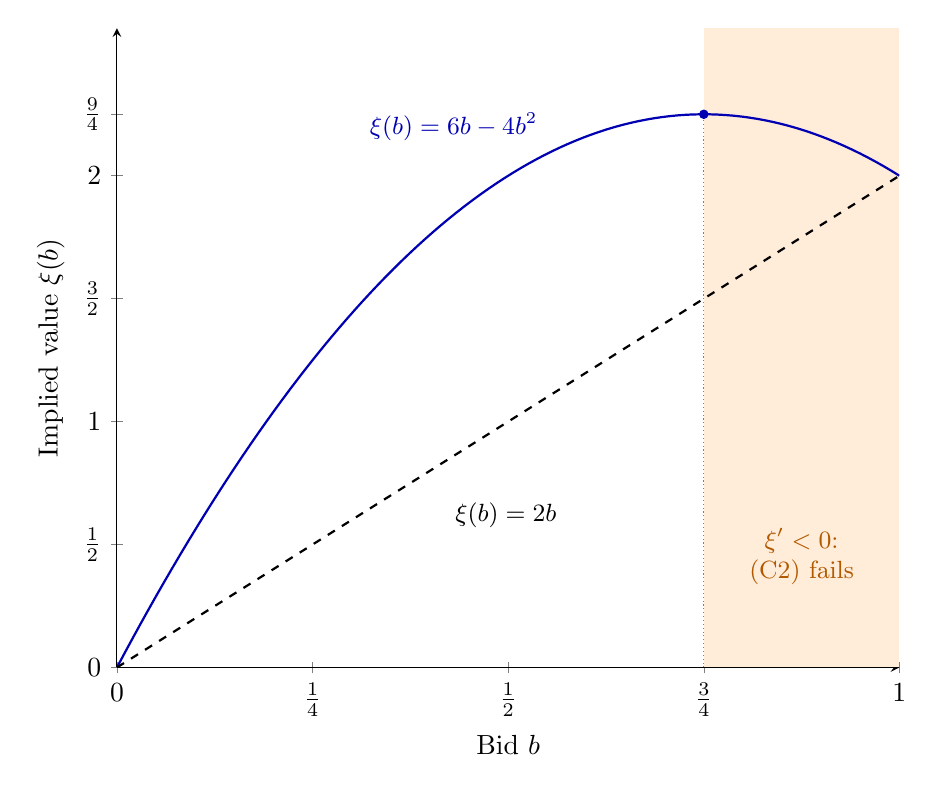
\begin{tikzpicture}
\begin{axis}[width=0.95\textwidth,height=0.8\textwidth,xmin=0,xmax=1,ymin=0,ymax=2.6,
  xlabel={Bid $b$},ylabel={Implied value $\xi(b)$},axis lines=left,
  xtick={0,0.25,0.5,0.75,1},xticklabels={$0$,$\frac14$,$\frac12$,$\frac34$,$1$},
  ytick={0,0.5,1,1.5,2,2.25},yticklabels={$0$,$\frac12$,$1$,$\frac32$,$2$,$\frac94$}]
\fill[orange!15] (axis cs:0.75,0) rectangle (axis cs:1,2.6);
\addplot[thick,blue!70!black,domain=0:1,samples=100] {6*x-4*x^2};
\addplot[thick,black,dashed,domain=0:1] {2*x};
\addplot[only marks,mark=*,mark size=1.5pt,blue!70!black] coordinates {(0.75,2.25)};
\draw[densely dotted,gray] (axis cs:0.75,0) -- (axis cs:0.75,2.25);
\node[font=\small,blue!70!black,anchor=east] at (axis cs:0.55,2.2) {$\xi(b)=6b-4b^2$};
\node[font=\small,anchor=west] at (axis cs:0.42,0.62) {$\xi(b)=2b$};
\node[font=\small,align=center,orange!70!black] at (axis cs:0.875,0.45) {$\xi'<0$:\\(C2) fails};
\end{axis}
\end{tikzpicture}
\caption{Inverse bid functions}
\end{subfigure}
\caption{The counterexample of \citet[p.~530]{GuerrePerrigneVuong2000}. Two bidders, bids i.i.d.\ with $G(b)=(\frac{b}{5-4b})^{\frac15}$ on $[0,1]$ (solid), against bids uniform on $[0,1]$ (dashed). The U-shaped bid density in panel (a) implies an inverse bid function that falls for $b>\frac34$ (shaded region in panel (b)), so no value distribution rationalizes these bids. Uniform bids imply $\xi(b)=2b$ and values uniform on $[0,2]$.}\label{fig:15-gpv-counter}
\end{figure}

\begin{remark}[What kind of identification result this is]\label{rem:15-gpv-ident-kind}
Four features of \cref{thm:15-gpv-ident} deserve emphasis. First, identification is nonparametric: no family of distributions is assumed. It implies identification within any parametric family. A parametric specification then serves only as an approximation and plays no role in identification (\cref{sec:15-identification}). Second, the proof is constructive, since \eqref{eq:15-gpv-F} gives $F$ explicitly. Third, the result is global. It does not rest on conditions in a neighborhood of a particular distribution \citep[footnote 7]{GuerrePerrigneVuong2000}. Fourth, the theorem characterizes the testable content of the model: (C1) and (C2) are all the restrictions that the SIPV first-price model places on bids from auctions with a fixed $n$. \Cref{sec:15-gpv-tests} turns them into tests.
\end{remark}

\begin{remark}[One equilibrium in all auctions]\label{rem:15-gpv-same-eq}
The inversion uses the distribution of rival bids observed across auctions as the belief of each bidder in each auction. This relies on the sampling assumption of \cref{sec:15-primitives} that the same equilibrium is played in all auctions with the same observables. In the SIPV model the equilibrium is unique, so the assumption holds automatically \citep[Section 3.1]{AtheyHaile2007}.
\end{remark}

\subsection{The bid density is smoother than the value density}\label{sec:15-gpv-smooth}

The estimator of \cref{sec:15-gpv-estimator} replaces $G$ and $g$ in \eqref{eq:15-gpv-xi} by estimates. How well they can be estimated depends on their smoothness. GPV show that the bid density has one more derivative than the value density.

\begin{proposition}[\citealp{GuerrePerrigneVuong2000}, Proposition 1]\label{prop:15-gpv-smooth}
Under \cref{ass:15-gpv-regularity}, the conditional bid distribution $G(\cdot\mid\cdot,\cdot)$ satisfies the following.
(i) For each $n\in\mathcal I$, its support is $\{(b,z):z\in[\underline z,\bar z],\ b\in[\underline b(z,n),\bar b(z,n)]\}$ with $\inf_z[\bar b(z,n)-\underline b(z,n)]>0$. The boundaries $\underline b(\cdot,n)$ and $\bar b(\cdot,n)$ have $R+1$ continuous bounded derivatives, and $\underline b(z,n)=\underline v(z)$.
(ii) $g(b\mid z,n)\ge c_g>0$ on the support.
(iii) $G(\cdot\mid\cdot,n)$ has $R+1$ continuous bounded partial derivatives on the support.
(iv) On any closed subset of the interior of the support, $g(\cdot\mid\cdot,n)$ has $R+1$ continuous bounded partial derivatives.
\end{proposition}

Part (iv) is the striking one. The value density has $R$ derivatives, and the bid density has $R+1$ on inner sets. The intuition comes from rearranging \eqref{eq:15-gpv-xi}:
\begin{equation}\label{eq:15-gpv-g-from-xi}
g(b\mid z,n)=\frac{G(b\mid z,n)}{(n-1)\big(\xi(b;z,n)-b\big)}
\end{equation}
\citep[p.~536]{GuerrePerrigneVuong2000}. The same formula appeared in \cref{sec:15-ml} as the bid density of a parametric model. The bid function \eqref{eq:15-gpv-rs} involves $F$ and its integral, so it has the $R+1$ derivatives of $F$. Its inverse $\xi$ inherits them. The distribution $G$ also has $R+1$ derivatives by part (iii). On inner sets the denominator of \eqref{eq:15-gpv-g-from-xi} is bounded away from zero, so $g$ has $R+1$ derivatives there. The bidding strategy acts as a smoothing operator. Each bid aggregates information about the whole lower tail of $F$ through the integral in \eqref{eq:15-gpv-rs}.

Formula \eqref{eq:15-gpv-g-from-xi} also explains part (ii) and the behavior of $g$ at the edges of its support. At the top, $G(\bar b)=1$, so $g(\bar b)=\frac{1}{(n-1)(\bar v-\bar b)}$. At the bottom, both $G$ and $\xi(b)-b$ vanish. To find the limit we expand near $\underline v$. Because $f(\underline v)>0$, we have $F(u)=f(\underline v)(u-\underline v)(1+o(1))$ as $u\downarrow\underline v$. Substituting into \eqref{eq:15-gpv-rs},
\[
v-\beta(v)=\frac{\int_{\underline v}^vf(\underline v)^{n-1}(u-\underline v)^{n-1}du}{f(\underline v)^{n-1}(v-\underline v)^{n-1}}\big(1+o(1)\big)=\frac{v-\underline v}{n}\big(1+o(1)\big).
\]
Hence, at $b=\beta(v)$,
\[
g(b)=\frac{F(v)}{(n-1)\big(v-\beta(v)\big)}=\frac{f(\underline v)(v-\underline v)}{(n-1)\frac{v-\underline v}{n}}\big(1+o(1)\big)\longrightarrow\frac{n}{n-1}\,f(\underline v)
\]
as $v\downarrow\underline v$. For values uniform on $[0,1]$, bids are uniform on $[0,\frac{n-1}{n}]$ with density $\frac{n}{n-1}$, which matches the formula.

The consequence for estimation is immediate. By \citet{Stone1982}, a function with $R+1$ derivatives in $d+1$ dimensions can be estimated uniformly at the rate $(\frac{T}{\log T})^{\frac{R+1}{2R+d+3}}$. The bid density, and with it the inverse bid function on inner sets, can therefore be estimated faster than the value density could be estimated even if values were observed. The difficulty lies elsewhere, as \cref{sec:15-gpv-rates} shows.

\subsection{The two-step estimator}\label{sec:15-gpv-estimator}

\Cref{thm:15-gpv-ident} suggests an estimator that mirrors identification. In the first step we estimate $G$ and $g$ nonparametrically and use \eqref{eq:15-gpv-xi} to build a \emph{pseudo-sample} of values, one pseudo-value per bid (\cref{sec:15-routes}). In the second step we treat the pseudo-values as a sample from $F$ and estimate its density by kernel smoothing. Kernel density estimation, bandwidths and boundary effects are reviewed in \cref{app:econometrics}. Throughout, kernels are normalized to have support $[-1,1]$.

\casehead{Homogeneous auctions} Suppose first that all $T$ auctions sell identical objects with the same number $n$ of bidders. The first step estimates the bid distribution by its empirical counterpart and the bid density by a kernel estimator (GPV, eqs.~(4)--(5)):
\begin{align}
\hat G(b)&=\frac{1}{nT}\sum_{t=1}^T\sum_{i=1}^n\indic(B_{it}\le b),\label{eq:15-gpv-Ghat}\\
\hat g(b)&=\frac{1}{nTh_g}\sum_{t=1}^T\sum_{i=1}^n\mathcal K\Big(\frac{b-B_{it}}{h_g}\Big),\label{eq:15-gpv-ghat}
\end{align}
where $\mathcal K$ is a kernel and $h_g$ a bandwidth. All $nT$ bids enter, because bids are i.i.d.\ within and across auctions under (C1).

\casehead{Boundary bias} A kernel density estimator is biased near the edges of the support, and the bias contaminates the pseudo-values. We derive the bias at the top of the support, following GPV, p.~531. Take a symmetric kernel with support $[-1,1]$ and a bid $b=\bar b-\lambda h_g$ with $\lambda\in[0,1)$. Then
\[
\E\big[\hat g(b)\big]=\frac{1}{h_g}\int_{\underline b}^{\bar b}\mathcal K\Big(\frac{b-y}{h_g}\Big)g(y)\,dy.
\]
We change variables to $u=\frac{b-y}{h_g}$, so that $y=b-h_gu$ and $dy=-h_g\,du$. The upper limit $y=\bar b$ becomes $u=\frac{b-\bar b}{h_g}=-\lambda$. The lower limit $y=\underline b$ becomes $u=\frac{b-\underline b}{h_g}$, which exceeds one once $h_g$ is small. Hence
\[
\E\big[\hat g(b)\big]=\int_{-\lambda}^{1}\mathcal K(u)\,g(b-h_gu)\,du\longrightarrow g(\bar b)\int_{-\lambda}^{1}\mathcal K(u)\,du\qquad\text{as }h_g\to0.
\]
For $\lambda<1$ the integral of the kernel is less than one, and at $\lambda=0$ it equals $\frac12$. Within one bandwidth of $\bar b$, the estimator therefore underestimates the density, by up to one half at the edge. The same argument applies within one bandwidth of $\underline b$.

The effect on the pseudo-values is large. At the top, $\hat G\approx1$ while $\hat g\approx\frac12g(\bar b)$, so the estimated markdown is about twice the true markdown $\bar v-\bar b$. The pseudo-value of the top bid is then about $\bar b+2(\bar v-\bar b)=2\bar v-\bar b$, well above the largest possible value. \Cref{fig:15-gpv-trim} shows the effect in a simulated sample.

\casehead{Trimming} Let $B_{\min}$ and $B_{\max}$ be the smallest and largest of the $nT$ bids. Because $\underline b\le B_{\min}$ and $B_{\max}\le\bar b$, the estimator $\hat g$ is asymptotically unbiased on $[B_{\min}+h_g,B_{\max}-h_g]$. GPV define the pseudo-values as (GPV, eq.~(6))
\begin{equation}\label{eq:15-gpv-trim}
\hat V_{it}=\begin{cases}
B_{it}+\dfrac{1}{n-1}\,\dfrac{\hat G(B_{it})}{\hat g(B_{it})}&\text{if }B_{\min}+h_g\le B_{it}\le B_{\max}-h_g,\\[2ex]
+\infty&\text{otherwise.}
\end{cases}
\end{equation}
Setting a trimmed pseudo-value to $+\infty$ removes it from the second step, because a kernel with bounded support assigns it zero weight.

\casehead{Second step} The density of values is estimated by (GPV, eq.~(7))
\begin{equation}\label{eq:15-gpv-fhat}
\hat f(v)=\frac{1}{nTh_f}\sum_{t=1}^T\sum_{i=1}^n\mathcal K_f\Big(\frac{v-\hat V_{it}}{h_f}\Big),
\end{equation}
with kernel $\mathcal K_f$ and bandwidth $h_f$. The distribution function, quantiles, and any functional of $F$ follow from the pseudo-values or from $\hat f$. The estimator involves no optimization and no equilibrium computation.

\casehead{Heterogeneous auctions} In applications the objects differ and the number of bidders varies. GPV, Section 3.3, extend the estimator jointly over $(b,z,n)$. Define
\[
G(b,z,n)=G(b\mid z,n)f_{Zn}(z,n),\qquad g(b,z,n)=g(b\mid z,n)f_{Zn}(z,n).
\]
The density $f_{Zn}$ cancels in the ratio, so \eqref{eq:15-gpv-xi} becomes (GPV, eq.~(12))
\begin{equation}\label{eq:15-gpv-psi}
V_{it}=B_{it}+\frac{1}{n_t-1}\,\psi(B_{it},Z_t,n_t),\qquad\psi(b,z,n)\equiv\frac{G(b,z,n)}{g(b,z,n)}.
\end{equation}
The ratio $\psi$ is a local symbol of this subsection, unrelated to the virtual valuation $\psi$ of \eqref{eq:14-psi}. The numerator and denominator are estimated by (GPV, eqs.~(13)--(14))
\begin{align}
\hat G(b,z,n)&=\frac{1}{Th_G^d}\sum_{t=1}^T\frac{1}{n_t}\sum_{i=1}^{n_t}\indic(B_{it}\le b)\,\mathcal K_G\Big(\frac{z-Z_t}{h_G},\frac{n-n_t}{h_{Gn}}\Big),\label{eq:15-gpv-Ghat-z}\\
\hat g(b,z,n)&=\frac{1}{Th_g^{d+1}}\sum_{t=1}^T\frac{1}{n_t}\sum_{i=1}^{n_t}\mathcal K_g\Big(\frac{b-B_{it}}{h_g},\frac{z-Z_t}{h_g},\frac{n-n_t}{h_{gn}}\Big).\label{eq:15-gpv-ghat-z}
\end{align}
The factor $\frac{1}{n_t}$ averages the bids within an auction, because $\E\big[\frac{1}{n_t}\sum_i\indic(B_{it}\le b)\mid Z_t,n_t\big]=G(b\mid Z_t,n_t)$. The kernels are products of kernels in each argument. The discrete variable $n$ receives its own bandwidths $h_{Gn}$ and $h_{gn}$, which vanish as $T$ grows, so that asymptotically only auctions with $n_t=n$ contribute \citep{Bierens1987}. With discrete covariates one estimates cell by cell, and $d$ counts only the continuous covariates \citep[footnote 12]{GuerrePerrigneVuong2000}.

\casehead{Estimated boundaries and trimming} The support of bids now varies with $(z,n)$ and is unknown. Even if $\underline v(\cdot)$ and $\bar v(\cdot)$ were known, $\bar b(z,n)=\beta(\bar v(z);z,n)$ would depend on $F$. GPV partition $\R^d$ into hypercubes of side $h_\partial$ and estimate (GPV, eqs.~(16)--(17))
\begin{align*}
\hat{\bar b}(z,n)&=\max\{B_{it}:\ Z_t\text{ in the hypercube containing }z,\ n_t=n\},\\
\hat{\underline b}(z)&=\min\{B_{it}:\ Z_t\text{ in the hypercube containing }z\}.
\end{align*}
The lower estimate pools all $n$, because $\underline b(z,n)=\underline v(z)$ does not depend on $n$. Let $\hat S_n=\{(b,z):z\in[\underline z,\bar z],\ b\in[\hat{\underline b}(z),\hat{\bar b}(z,n)]\}$ be the estimated support, and let $S(h)=[-h,h]^{d+1}$ denote the support of a kernel on $[-1,1]^{d+1}$ rescaled by $h$, a hypercube of side $2h$ centered at the origin. The kernel $\mathcal K_G$ does not smooth over bids, so for it GPV set the bid coordinate to zero, $S(h_G)=\{0\}\times[-h_G,h_G]^d$. The pseudo-value is $\hat V_{it}=B_{it}+\frac{1}{n_t-1}\hat\psi(B_{it},Z_t,n_t)$ with (GPV, eqs.~(18)--(19))
\begin{equation}\label{eq:15-gpv-trim-z}
\hat\psi(b,z,n)=\begin{cases}
\dfrac{\hat G(b,z,n)}{\hat g(b,z,n)}&\text{if }(b,z)+S(2h_G)\subset\hat S_n\text{ and }(b,z)+S(2h_g)\subset\hat S_n,\\[2ex]
+\infty&\text{otherwise.}
\end{cases}
\end{equation}
An observation is trimmed when the cube of half-width $2h_g$ centered at it leaves the estimated support, or when the corresponding cube of half-width $2h_G$ in the covariates does. Without covariates, the factor 2 can be replaced by 1. The condition $b+S(h_g)\subset[B_{\min},B_{\max}]$ then reads $B_{\min}+h_g\le b\le B_{\max}-h_g$, which returns \eqref{eq:15-gpv-trim} \citep[footnote 20]{GuerrePerrigneVuong2000}.

\casehead{Second step with covariates} The conditional density of values is the ratio $\hat f(v\mid z)=\frac{\hat f(v,z)}{\hat f(z)}$, where (GPV, eqs.~(20)--(21))
\begin{align}
\hat f(v,z)&=\frac{1}{Th_f^{d+1}}\sum_{t=1}^T\frac{1}{n_t}\sum_{i=1}^{n_t}\mathcal K_f\Big(\frac{v-\hat V_{it}}{h_f},\frac{z-Z_t}{h_f}\Big),\label{eq:15-gpv-fhat-z}\\
\hat f(z)&=\frac{1}{Th_Z^d}\sum_{t=1}^T\mathcal K_Z\Big(\frac{z-Z_t}{h_Z}\Big).\notag
\end{align}
The second step pools auctions with different $n$. This presumes that values and the number of bidders are independent given $Z_t$, so that $f(v\mid z,n)=f(v\mid z)$. GPV adopt this restriction and note that its failure calls for an explicit model of entry \citep[footnote 14]{GuerrePerrigneVuong2000}. \Cref{sec:15-entry} develops such models.

\begin{assumption}[Kernels and bandwidths, GPV Assumptions A3--A4]\label{ass:15-gpv-bandwidth}
(i) The kernels $\mathcal K_G$, $\mathcal K_g$, $\mathcal K_f$ and $\mathcal K_Z$ are symmetric with bounded hypercube supports, integrate to one, and have two continuous bounded derivatives in their continuous arguments. Their orders are $R+1$, $R+1$, $R$ and $R+1$, so that their moments of lower order vanish.
(ii) The discrete bandwidths $h_{Gn}$ and $h_{gn}$ vanish as $T\to\infty$.
(iii) For positive constants $c_G,c_g,c_f,c_Z,c_\partial$,
\begin{align*}
h_G&=c_G\Big(\frac{\log T}{T}\Big)^{\frac{1}{2R+d+2}}, & h_g&=c_g\Big(\frac{\log T}{T}\Big)^{\frac{1}{2R+d+3}},\\
h_f&=c_f\Big(\frac{\log T}{T}\Big)^{\frac{1}{2R+d+3}}, & h_Z&=c_Z\Big(\frac{\log T}{T}\Big)^{\frac{1}{2R+d+2}},
\end{align*}
and, when $d>0$, $h_\partial=c_\partial\big(\frac{\log T}{T}\big)^{\frac{1}{d+1}}$.
\end{assumption}

The bandwidths for $G$, $g$ and $f(z)$ are the uniformly optimal choices for functions with $R+1$ derivatives. A function of $d$ arguments with $R+1$ derivatives calls for the exponent $\frac{1}{2(R+1)+d}=\frac{1}{2R+d+2}$. The bid density has $d+1$ arguments, which gives $\frac{1}{2R+d+3}$. The factor $\log T$ appears because the results concern uniform convergence. The choice of $h_f$ is unusual. If values were observed, the optimal exponent for $f(\cdot,\cdot)$ would be $\frac{1}{2R+d+1}$, and $h_f$ would shrink faster. The prescribed $h_f$ is larger, so the second step \emph{oversmooths}. \Cref{sec:15-gpv-rates} explains why this is the only rate that attains the optimal convergence rate.

\casehead{Bandwidths in practice} GPV's Monte Carlo uses $R=1$ and $d=0$, so both $h_g$ and $h_f$ are of order $T^{-\frac15}$ up to the logarithm. They use the triweight kernel
\[
\mathcal K(u)=\frac{35}{32}\big(1-u^2\big)^3\indic(|u|\le1)
\]
for both steps, with $h_g=1.06\,\hat\sigma_b(nT)^{-\frac15}$ and $h_f=1.06\,\hat\sigma_v(nT_T)^{-\frac15}$ \citep[p.~532]{GuerrePerrigneVuong2000}. Here $\hat\sigma_b$ and $\hat\sigma_v$ are the standard deviations of the bids and of the pseudo-values that survive trimming, which GPV call the trimmed pseudo private values. $T_T$ is the number of auctions left after trimming. The factor 1.06 is the Gaussian rule of thumb \citep{Hardle1991}.

Later work multiplies the rule by $2.978$ when it uses the triweight kernel \citep{LiPerrigneVuong2002,CampoPerrigneVuong2003,Krasnokutskaya2011}. The factor converts a bandwidth that is optimal for the Gaussian kernel into the equivalent bandwidth for the triweight kernel. We verify it. For a second-order kernel, the bandwidth that minimizes the asymptotic mean integrated squared error is proportional to the kernel constant $\delta_{\mathcal K}=\big(\frac{\int\mathcal K^2}{(\int u^2\mathcal K)^2}\big)^{\frac15}$. The factor of proportionality does not depend on the kernel \citep{Hardle1991}. For the Gaussian kernel, $\int\mathcal K^2=\frac{1}{2\sqrt\pi}$ and $\int u^2\mathcal K=1$, so $\delta=(2\sqrt\pi)^{-\frac15}\approx0.7764$. For the triweight kernel,
\[
\int_{-1}^1\mathcal K^2=\Big(\frac{35}{32}\Big)^2\int_{-1}^1(1-u^2)^6du=\frac{350}{429},\qquad\int_{-1}^1u^2\mathcal K=\frac{35}{32}\int_{-1}^1u^2(1-u^2)^3du=\frac19,
\]
so $\delta=\big(\frac{350}{429}\cdot81\big)^{\frac15}\approx2.3122$. The ratio is $\frac{2.3122}{0.7764}\approx2.978$. GPV's choice, without the factor, is narrower than the Gaussian-equivalent bandwidth. It trims fewer bids and smooths less. \Cref{tab:15-gpv-mc} compares the two choices.

\casehead{The algorithm} For a sample of first-price auctions with all bids recorded, the estimator proceeds as follows.
\begin{enumerate}
\item Group auctions by the number of bidders, and by covariate cells if covariates are discrete. Choose kernels and bandwidths, for example by the rule of thumb above.
\item For each bid, compute $\hat G(B_{it})$ and $\hat g(B_{it})$ from \eqref{eq:15-gpv-Ghat}--\eqref{eq:15-gpv-ghat}, or from \eqref{eq:15-gpv-Ghat-z}--\eqref{eq:15-gpv-ghat-z} with continuous covariates.
\item Trim the bids within one bandwidth of the estimated boundaries, and compute the pseudo-values of the remaining bids from \eqref{eq:15-gpv-trim} or \eqref{eq:15-gpv-trim-z}.
\item Evaluate $\hat\xi(b)=b+\frac{\hat G(b)}{(n-1)\hat g(b)}$ on a grid and check that it is increasing, as (C2) requires.
\item Estimate the value density by \eqref{eq:15-gpv-fhat} or \eqref{eq:15-gpv-fhat-z}, and compute the functionals of interest. Examples are value quantiles, the winner's informational rent $\frac{V-B}{V}$, the optimal reserve price from $\hat F$ (\cref{cor:14-optimal-reserve}), and expected revenue under other formats, such as $\E[V^{(n-1:n)}]$ for a second-price auction.
\end{enumerate}

\subsection{Rates of convergence and inference*}\label{sec:15-gpv-rates}

How fast can any estimator recover $f(\cdot\mid z)$ from bids? GPV answer with the minimax theory of \citet{IbragimovHasminskii1981}. We state the criterion, the result, and a sketch of the proof. Let $\mathcal C$ be a compact subset, with nonempty interior, of the interior of the support of $f_0(v,z)$. For a candidate rate $r_T\to\infty$, consider (GPV, eq.~(10))
\begin{equation}\label{eq:15-gpv-minimax}
\inf_{\hat f}\ \sup_{f\in U_\epsilon(f_0)}\Pr_f\Big(r_T\sup_{(v,z)\in\mathcal C}\big|\hat f(v\mid z)-f(v\mid z)\big|>\kappa\Big),
\end{equation}
where the infimum runs over all estimators based on bids. Here $\Pr_f$ is the law of the observables when values have density $f$. The neighborhood $U_\epsilon(f_0)$ contains the densities that satisfy \cref{ass:15-gpv-regularity}, lie within $\epsilon$ of $f_0$ in sup norm, and have derivatives up to order $R$ bounded by a constant $M$. Taking the supremum over a neighborhood rules out estimators that do well at one density only. If $r_T$ grows too fast, \eqref{eq:15-gpv-minimax} stays bounded away from zero for every estimator. The optimal uniform rate is the fastest $r_T$ for which some estimator drives \eqref{eq:15-gpv-minimax} to zero for large $\kappa$.

\begin{theorem}[\citealp{GuerrePerrigneVuong2000}, Theorems 2 and 3]\label{thm:15-gpv-rate}
Let \cref{ass:15-gpv-sampling} and \cref{ass:15-gpv-regularity} hold.
\begin{itemize}
\item[(i)] (Lower bound.) There is $\kappa>0$ such that, with $r_T=(\frac{T}{\log T})^{\frac{R}{2R+d+3}}$,
\[
\lim_{\epsilon\to0}\ \liminf_{T\to\infty}\ \inf_{\hat f}\ \sup_{f\in U_\epsilon(f_0)}\Pr_f\Big(r_T\sup_{(v,z)\in\mathcal C}\big|\hat f(v\mid z)-f(v\mid z)\big|>\kappa\Big)>0.
\]
\item[(ii)] (Attainment.) If, in addition, \cref{ass:15-gpv-bandwidth} holds, the two-step estimator satisfies, for every closed inner subset $\mathcal C$ of the support,
\[
\sup_{(v,z)\in\mathcal C}\big|\hat f(v\mid z)-f(v\mid z)\big|=O\Big(\Big(\frac{\log T}{T}\Big)^{\frac{R}{2R+d+3}}\Big)\quad\text{almost surely}.
\]
\end{itemize}
Hence $(\frac{T}{\log T})^{\frac{R}{2R+d+3}}$ is the optimal uniform rate for estimating $f(\cdot\mid\cdot)$ from bids, and the two-step estimator attains it.
\end{theorem}

If values were observed, the optimal uniform rate would be $(\frac{T}{\log T})^{\frac{R}{2R+d+1}}$ \citep{Stone1982}. Not observing values costs two units in the denominator of the exponent. The proof of part (i) adapts the argument of \citet{Khasminskii1976} and relies on \cref{thm:15-gpv-ident,prop:15-gpv-smooth}. We do not reproduce it.

\casehead{Where the loss comes from} Differentiating \eqref{eq:15-gpv-F} with respect to $v$ gives (GPV, eq.~(11))
\begin{equation}\label{eq:15-gpv-f-from-xi}
f(v\mid z,n)=\frac{g\big(\xi^{-1}(v;z,n)\mid z,n\big)}{\xi'\big(\xi^{-1}(v;z,n);z,n\big)}.
\end{equation}
Recovering $f$ requires the derivative $\xi'$, and by \eqref{eq:15-gpv-xi} this requires the derivative $g'$. The bid density has $R+1$ derivatives in $d+1$ arguments. By \citet{Stone1982}, the optimal uniform rate for the first derivative of such a function is $(\frac{T}{\log T})^{\frac{(R+1)-1}{2(R+1)+(d+1)}}=(\frac{T}{\log T})^{\frac{R}{2R+d+3}}$. Estimating $g'$ is the hardest part of the problem, and its rate is the rate for $f$. \Cref{tab:15-gpv-rates} compares the exponents.

\begin{table}[htbp]
\centering
\begin{threeparttable}
\caption{Exponents of the optimal uniform convergence rates $(\frac{T}{\log T})^{a}$}\label{tab:15-gpv-rates}
\small
\begin{tabular}{ccccc}
\toprule
$R$ & $d$ & \makecell{Values observed\\ $a=\frac{R}{2R+d+1}$} & \makecell{Bids only\\ $a=\frac{R}{2R+d+3}$} & \makecell{Pseudo-values, inner sets\\ $a=\frac{R+1}{2R+d+3}$}\\
\midrule
1 & 0 & $\frac13$ & $\frac15$ & $\frac25$\\[2pt]
2 & 0 & $\frac25$ & $\frac27$ & $\frac37$\\[2pt]
1 & 1 & $\frac14$ & $\frac16$ & $\frac13$\\[2pt]
2 & 1 & $\frac13$ & $\frac14$ & $\frac38$\\[2pt]
1 & 2 & $\frac15$ & $\frac17$ & $\frac27$\\
\bottomrule
\end{tabular}
\begin{tablenotes}
\footnotesize
\item \textit{Notes.} $R$ is the number of bounded derivatives of the value density and $d$ the number of continuous covariates. The column ``Values observed'' gives the rate of \citet{Stone1982}, and the column ``Bids only'' gives the rate of \cref{thm:15-gpv-rate}. The last column gives the rate of $\sup|\hat V_{it}-V_{it}|$ over bids away from the boundary (GPV, Proposition 3(ii)). Our computation from these formulas.
\end{tablenotes}
\end{threeparttable}
\end{table}

\casehead{Sketch of the proof of part (ii)} The argument shows why the second step must oversmooth. Write $\varepsilon_T=\frac{\log T}{T}$. Two preliminary results are needed. The boundary estimators converge at the rate $\varepsilon_T^{\frac{1}{d+1}}$ (GPV, Proposition 2). The untrimmed pseudo-values satisfy $\sup|\hat V_{it}-V_{it}|=O(\varepsilon_T^{\frac{R}{2R+d+3}})$, and on bids away from the boundary $\sup|\hat V_{it}-V_{it}|=O(\varepsilon_T^{\frac{R+1}{2R+d+3}})$ almost surely (GPV, Proposition 3). The faster inner rate reflects the extra derivative of $g$ in \cref{prop:15-gpv-smooth}.

Because $\hat f(z)$ converges at the faster rate $\varepsilon_T^{\frac{R+1}{2R+d+2}}$ and $f(z)$ is bounded away from zero, it suffices to study $\hat f(v,z)$. Let $\tilde f(v,z)$ be the infeasible estimator \eqref{eq:15-gpv-fhat-z} computed with the true values $V_{it}$ in place of $\hat V_{it}$ (GPV, eq.~(22)). We decompose
\[
\hat f(v,z)-f(v,z)=\big[\hat f(v,z)-\tilde f(v,z)\big]+\big[\tilde f(v,z)-f(v,z)\big].
\]
The second bracket is the error of an ordinary kernel estimator. Its bias is $O(h_f^R)$, since $\mathcal K_f$ has order $R$ and $f$ has $R$ derivatives. Its stochastic part is $O\big((\frac{\log T}{Th_f^{d+1}})^{\frac12}\big)$ uniformly. With $h_f\propto\varepsilon_T^{\frac{1}{2R+d+3}}$, these are
\[
h_f^R\propto\varepsilon_T^{\frac{R}{2R+d+3}},\qquad\Big(\frac{\varepsilon_T}{h_f^{d+1}}\Big)^{\frac12}\propto\varepsilon_T^{\frac12\left(1-\frac{d+1}{2R+d+3}\right)}=\varepsilon_T^{\frac{R+1}{2R+d+3}}.
\]
The bias dominates, and the second bracket is $O(\varepsilon_T^{\frac{R}{2R+d+3}})$.

For the first bracket, points $(v,z)$ in $\mathcal C$ use only observations whose true values lie in a slightly larger inner set, once $T$ is large. A second-order Taylor expansion of $\mathcal K_f$ in its first argument gives (GPV, eq.~(23))
\[
\big|\hat f(v,z)-\tilde f(v,z)\big|\le\frac{\sup|\hat V_{it}-V_{it}|}{h_f}\,A_T+\frac{\sup|\hat V_{it}-V_{it}|^2}{2h_f^3}\,B_T,
\]
where the suprema run over inner observations. The terms $A_T$ and $B_T$ are averages of the type $\frac{1}{Th_f^{d+1}}\sum_t|\partial_1\mathcal K_f(\cdot)|$ and $\frac{1}{Th_f^{d}}\sum_t\sup_v|\partial_1^2\mathcal K_f(\cdot)|$. Like kernel estimators, they stay bounded almost surely. Using the inner rate of Proposition 3, the first term is of order
\[
\frac{\varepsilon_T^{\frac{R+1}{2R+d+3}}}{\varepsilon_T^{\frac{1}{2R+d+3}}}=\varepsilon_T^{\frac{R}{2R+d+3}},
\]
and the second is of order $\varepsilon_T^{\frac{2(R+1)-3}{2R+d+3}}=\varepsilon_T^{\frac{2R-1}{2R+d+3}}$. Since $R\ge1$ implies $2R-1\ge R$, the second term is no larger than the first. Both brackets are therefore $O(\varepsilon_T^{\frac{R}{2R+d+3}})$, which proves part (ii).

The bookkeeping explains the choice of $h_f$. The first-step error enters as $\frac{\sup|\hat V-V|}{h_f}$, which falls as $h_f$ grows. The smoothing bias $h_f^R$ rises with $h_f$. Equating $\varepsilon_T^{\frac{R+1}{2R+d+3}}h_f^{-1}$ with $h_f^R$ gives $h_f^{R+1}=\varepsilon_T^{\frac{R+1}{2R+d+3}}$, that is $h_f\propto\varepsilon_T^{\frac{1}{2R+d+3}}$. Given the optimal first-step bandwidths, this is the only rate for $h_f$ that attains the optimal rate \citep[p.~546]{GuerrePerrigneVuong2000}. The usual choice $h_f\propto\varepsilon_T^{\frac{1}{2R+d+1}}$ would undersmooth relative to the first-step noise and give a slower rate.

\casehead{Inference} \Cref{thm:15-gpv-rate} gives rates of convergence. It says nothing about limiting distributions, and GPV do not establish asymptotic normality of $\hat f$. They note that the second-order term of the expansion can be close to the first when $R$ is small, so normal approximations based on the leading term may be inaccurate \citep[p.~546]{GuerrePerrigneVuong2000}. They suggest instead an exponential inequality of the form (GPV, eq.~(24))
\[
\Pr\Big(\Big(\frac{T}{\log T}\Big)^{\frac{R}{2R+d+3}}\sup_{(v,z)\in\mathcal C}\big|\hat f(v\mid z)-f(v\mid z)\big|>e^*(\tau)\Big)\le P^*(\tau),
\]
which would deliver conservative uniform bands $\hat f\pm e^*(\tau)(\frac{\log T}{T})^{\frac{R}{2R+d+3}}$ with coverage at least $1-P^*(\tau)$. The same inequality bounds the expected sup-norm loss and could guide the choice of the bandwidth constants. GPV leave the derivation of $e^*$ and $P^*$ to future work.

Practice has moved in two directions \citep[Section 3.2.1]{AtheyHaile2007}. First, many questions concern functionals of $F$, such as quantiles, expected revenue or the optimal reserve price. \Citet{HaileHongShum2003} show that the pseudo-values and fixed quantiles of their empirical distribution are asymptotically normal. Second, applied work uses the bootstrap. Outside the IPV model, bids are correlated within an auction. One therefore resamples whole auctions with replacement within each value of $n$ and recomputes both steps in each bootstrap sample. Subsampling is an alternative \citep{HaileHongShum2003}.

\subsection{A Monte Carlo illustration*}\label{sec:15-gpv-mc}

\casehead{GPV's design} GPV illustrate the estimator with a small Monte Carlo study \citep[Section 2.4]{GuerrePerrigneVuong2000}. Each replication has $T=200$ auctions with $n=5$ bidders, so 1,000 bids, which they describe as a realistic sample size. Values are lognormal with parameters zero and one, truncated to $[0.055,2.5]$. GPV say that the truncation leaves out ``20\% approximately'' of the original lognormal distribution (p.~532). Our calculation gives 18.2 percent, almost all of it above 2.5. The truncation makes the support compact as \cref{ass:15-gpv-regularity} requires. Bids are computed from \eqref{eq:15-gpv-rs} by numerical integration. The estimator uses $R=1$, triweight kernels in both steps, and the rule-of-thumb bandwidths described in \cref{sec:15-gpv-estimator}. There are 1,000 replications.

GPV report the results in two figures, without tables. Their Figure~1 plots the true equilibrium strategy with the mean and the 5th and 95th percentiles of the 1,000 estimates $\hat\xi(b)$, evaluated at 500 points on $[\beta(0.055),\beta(2.5)]$. Their Figure~2 does the same for the density on $[0.055,2.5]$. Inside the region delimited by the trimming, the true curves lie within the pointwise 90 percent bands and the mean estimates match them closely \citep[p.~533]{GuerrePerrigneVuong2000}. Each replication took less than a minute in FORTRAN. GPV estimate that a parametric nonlinear least squares estimator would take about 1,000 times longer, because it requires the numerical integration of \eqref{eq:15-gpv-rs} at every trial parameter \citep[p.~532]{GuerrePerrigneVuong2000}.

\casehead{Our replication} We replicate the design exactly, including the bandwidth rules with the factor 1.06 and 1,000 replications. The script \texttt{figures/ch15/src/gpv\_montecarlo.py} computes the true bid function by integrating \eqref{eq:15-gpv-rs} on a grid of 200,001 points, with seed 15401. \Cref{fig:15-gpv-mc} reports the results in the format of GPV's Figures 1 and 2. As in their footnote~9, the dotted lines mark the average trimming bounds $B_{\min}+h_g$ and $B_{\max}-h_g$ in panel (a). In panel (b) they mark the average of $\hat\xi(B_{\min}+h_g)+h_f$ and $\hat\xi(B_{\max}-h_g)-h_f$, which removes the remaining boundary effects of the second step.

\begin{figure}[htbp]
\centering
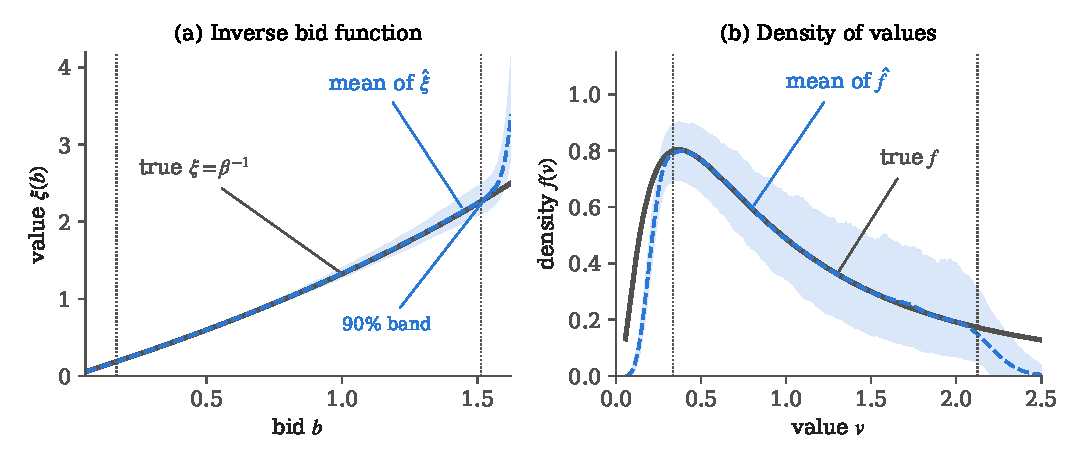
\includegraphics[width=\textwidth]{figures/ch15/gpv_mc.pdf}
\caption{Replication of the Monte Carlo design of \citet[Section 2.4]{GuerrePerrigneVuong2000}: $T=200$ auctions, $n=5$ bidders, values lognormal$(0,1)$ truncated to $[0.055,2.5]$, triweight kernels, $h_g=1.06\,\hat\sigma_b(nT)^{-\frac15}$, $h_f=1.06\,\hat\sigma_v(nT_T)^{-\frac15}$, 1,000 replications. Panel (a): true inverse bid function, mean of $\hat\xi(b)$ (dashed) and pointwise 90 percent band of the estimates. Panel (b): true value density, mean of $\hat f(v)$ and 90 percent band. Dotted lines mark the average trimming bounds. Our simulation (seed 15401), following the design of \citet[Section 2.4]{GuerrePerrigneVuong2000}.}\label{fig:15-gpv-mc}
\end{figure}

The replication reproduces GPV's qualitative findings. Inside the dotted lines the mean estimates are close to the truth, and the true curves lie inside the bands at every grid point. On the trimmed bid range, the mean of $\hat\xi$ is never more than 0.013 away from $\xi$. On the inner value region, the mean of $\hat f$ is never more than 0.022 away from $f$ (\cref{tab:15-gpv-mc}). The average trimming bounds on bids are 0.168 and 1.511, and the inner value region is $[0.334,2.125]$. Both are close to the lines drawn in GPV's figures. Outside these regions the estimates deteriorate as \cref{sec:15-gpv-estimator} predicts. Near the top of the bid support the mean of $\hat\xi$ bends sharply upward. Near both ends of the value support the mean of $\hat f$ falls below the truth.

\begin{figure}[htbp]
\centering
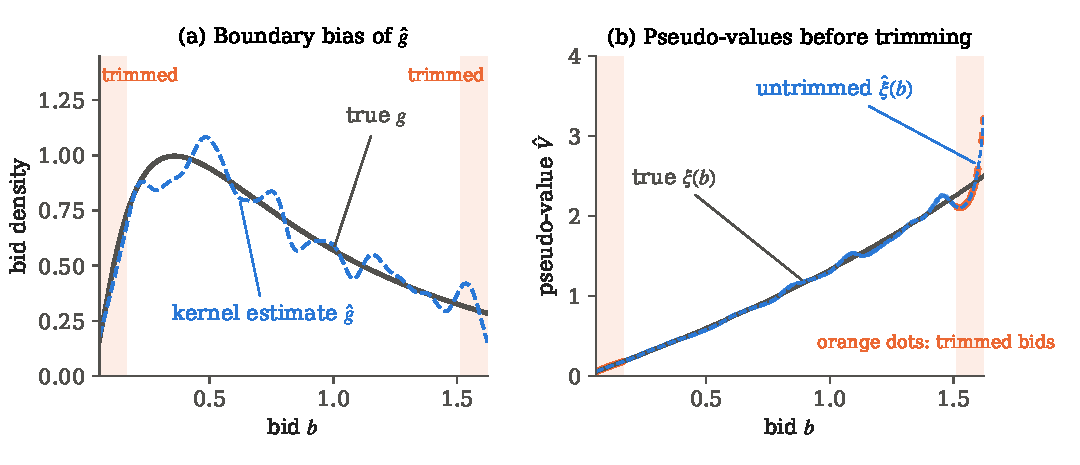
\includegraphics[width=\textwidth]{figures/ch15/gpv_trim.pdf}
\caption{Boundary effects in one simulated sample from the design of \cref{fig:15-gpv-mc} ($h_g=0.108$). Panel (a): true bid density and the triweight kernel estimate. Shaded areas lie within one bandwidth of the smallest and largest bids. At the largest bid the estimate equals 0.54 times the true density. Panel (b): pseudo-values $B_{it}+\frac{\hat G(B_{it})}{(n-1)\hat g(B_{it})}$ before trimming (dots), the estimated inverse bid function on a grid (dashed) and the true $\xi$ (solid). Near the top, the underestimated density inflates the markdown, and the estimated inverse bid function rises well above $\bar v=2.5$. Our simulation (seed 15403).}\label{fig:15-gpv-trim}
\end{figure}

\Cref{fig:15-gpv-trim} shows the mechanism in one sample. At the largest bid, $\hat g$ is 0.54 times the true density, close to the factor $\frac12$ derived in \cref{sec:15-gpv-estimator}. The untrimmed estimate $\hat\xi$ climbs to about 3.2 at the top of the bid support, against a true maximum value of 2.5. Trimming removes 43 of the 1,000 bids at the top. Among the bids that survive trimming, the mean absolute error of the pseudo-values is 0.016.

\begin{table}[htbp]
\centering
\caption{Monte Carlo results for the GPV estimator}\label{tab:15-gpv-mc}
\small
\begin{tabular}{lcc}
\toprule
\multicolumn{3}{l}{\textit{Panel A. GPV design, $T=200$, $n=5$, 1,000 replications}}\\
\midrule
Bandwidth constant & $1.06$ (GPV) & $2.978\times1.06$ \\
\midrule
Mean $h_g$ & 0.107 & 0.320\\
Mean $h_f$ & 0.147 & 0.334\\
Share of bids trimmed & 0.088 & 0.363\\
Mean trimming bounds on bids & $[0.168,\,1.511]$ & $[0.380,\,1.299]$\\
Inner value region & $[0.334,\,2.125]$ & $[0.781,\,1.508]$\\
Max.\ $|$mean of $\hat\xi-\xi|$ on trimmed bids & 0.013 & 0.003\\
Max.\ $|$mean of $\hat f-f|$ on inner values & 0.022 & 0.006\\
Mean sup-norm error of $\hat\xi$ on trimmed bids & 0.161 & 0.043\\
Mean sup-norm error of $\hat f$ on inner values & 0.238 & 0.055\\
Seconds per replication (Python) & 0.028 & 0.076\\
\bottomrule
\end{tabular}

\medskip
\begin{tabular}{rcccc}
\toprule
\multicolumn{5}{l}{\textit{Panel B. Mean sup-norm errors on fixed inner sets, GPV bandwidths, 200 replications}}\\
\midrule
$T$ & \makecell{$\hat\xi$, bids\\ in $[0.25,1.35]$} & \makecell{$\hat f$, values\\ in $[0.4,1.8]$} & \makecell{$\tilde f$\\ (true values)} & Ratio $\frac{\hat f}{\tilde f}$\\
\midrule
100 & 0.149 & 0.243 & 0.128 & 1.89\\
200 & 0.113 & 0.227 & 0.102 & 2.21\\
400 & 0.087 & 0.203 & 0.080 & 2.54\\
800 & 0.067 & 0.176 & 0.064 & 2.73\\
1,600 & 0.053 & 0.152 & 0.049 & 3.07\\
\midrule
Log-log slope in $T$ & $-0.37$ & $-0.17$ & $-0.34$ & \\
\bottomrule
\end{tabular}

\smallskip
\begin{minipage}{0.9\textwidth}
\footnotesize
\textit{Notes.} Our simulation, script \texttt{figures/ch15/src/gpv\_montecarlo.py}, seeds 15401 (panel A) and 15402 (panel B). Values lognormal$(0,1)$ truncated to $[0.055,2.5]$, $n=5$, triweight kernels. In panel A the two columns use the same draws. The inner value region is the average of $[\hat\xi(B_{\min}+h_g)+h_f,\ \hat\xi(B_{\max}-h_g)-h_f]$, so the error rows of the two columns refer to different regions. In panel B, $\tilde f$ is the infeasible kernel estimator computed from the true values with the same kernel and rule-of-thumb bandwidth. Slopes are least-squares fits of the log error on $\log T$. Timings are from one run on a laptop and vary across runs.
\end{minipage}
\end{table}

Panel A of \cref{tab:15-gpv-mc} compares GPV's bandwidths with the Gaussian-equivalent bandwidths. The wider bandwidths cut the sup-norm errors by a factor of about four. They do so at a price: 36 percent of the bids are trimmed, and the inner value region shrinks to $[0.781,1.508]$. The tails of $F$, which matter for reserve prices and for the top of the bid distribution, are then not estimated at all. The trade-off between precision in the middle and coverage of the support is a practical feature of every application of the method.

Panel B illustrates \cref{thm:15-gpv-rate}. On fixed inner sets, the error of $\hat f$ falls more slowly with $T$ than the error of the infeasible estimator that uses true values. The ratio of the two errors rises from 1.9 at $T=100$ to 3.1 at $T=1{,}600$. The fitted slope for $\hat f$ is $-0.17$, close to the exponent $-\frac15$ that the theorem gives for $R=1$ and $d=0$. The slope for $\tilde f$ is $-0.34$. The inverse bid function requires $g$ without its derivative, and its error falls at the faster slope of $-0.37$. The design has a very smooth density, so these slopes illustrate the theory. They are no test of it. The whole experiment takes a few minutes on a laptop, which makes the computational case for the indirect approach plain.

\subsection{Binding reserve prices and unknown numbers of potential bidders}\label{sec:15-gpv-reserve}

In practice sellers often announce a reserve price high enough to screen out some bidders. GPV, Section 4, extend their results to this case. A binding reserve price creates a new unknown. Let $N$ denote the number of \emph{potential bidders}, who draw values and decide whether to bid. Let $n^*$ denote the number of \emph{actual bidders}, who submit a bid of at least $r$. The econometrician observes $n^*$ but typically not $N$. Following GPV, bidders do not observe which rivals participate when they bid.

\casehead{The inverse bid function with a reserve} Fix one auction with reserve price $r\in(\underline v,\bar v)$. Bidders with values below $r$ do not bid, and bidders with values $v\ge r$ bid $\beta(v)$ from \eqref{eq:14-rs-bid}, with $\beta(r)=r$. Let $G^*$ denote the distribution of an actual bid, with density $g^*$ on $[r,\bar b]$. Then
\[
G^*(b)=\Pr\big(\beta(V)\le b\bigm| V\ge r\big)=\frac{F\big(\beta^{-1}(b)\big)-F(r)}{1-F(r)}.
\]
We derive the analog of \eqref{eq:15-gpv-xi} from the bidder's problem. A bid $b\ge r$ beats a given rival if that rival's value is below $r$, which has probability $F(r)$, or if the rival bids but bids less than $b$, which has probability $(1-F(r))G^*(b)$. Rivals are independent, so the win probability is
\[
H(b)=\Big[F(r)+\big(1-F(r)\big)G^*(b)\Big]^{N-1}.
\]
The bidder maximizes $(v-b)H(b)$. The first-order condition is
\[
(v-b)(N-1)\Big[F(r)+\big(1-F(r)\big)G^*(b)\Big]^{N-2}\big(1-F(r)\big)g^*(b)=\Big[F(r)+\big(1-F(r)\big)G^*(b)\Big]^{N-1}.
\]
Dividing by $(N-1)[F(r)+(1-F(r))G^*(b)]^{N-2}(1-F(r))g^*(b)$ and adding $b$ gives
\[
v=b+\frac{F(r)+\big(1-F(r)\big)G^*(b)}{(N-1)\big(1-F(r)\big)g^*(b)}.
\]
Splitting the fraction yields GPV's equation~(25):
\begin{equation}\label{eq:15-gpv-reserve}
v=\xi\big(b;G^*,N,F(r)\big)\equiv b+\frac{1}{N-1}\Big(\frac{G^*(b)}{g^*(b)}+\frac{F(r)}{1-F(r)}\,\frac{1}{g^*(b)}\Big).
\end{equation}
The second term in the parentheses reflects the potential bidders who do not bid. Ignoring it understates the markdown, especially near $r$, where $G^*$ is small. Unlike \eqref{eq:15-gpv-xi}, equation \eqref{eq:15-gpv-reserve} involves two unknowns, $N$ and $F(r)$.

\casehead{Why the bid density is unbounded at the reserve} By \eqref{eq:15-gpv-ode} with $N$ bidders, $\beta'(v)=(N-1)\frac{f(v)}{F(v)}\big(v-\beta(v)\big)$. At $v=r$ the markdown $v-\beta(v)$ vanishes while $F(r)>0$, so $\beta'(r)=0$. Let $\Delta(v)=v-\beta(v)$. Then $\Delta(r)=0$ and $\Delta'(r)=1-\beta'(r)=1$, so $\Delta(v)=(v-r)(1+o(1))$. Substituting,
\[
\beta'(v)=(N-1)\frac{f(r)}{F(r)}(v-r)\big(1+o(1)\big),\qquad\beta(v)-r=\frac{(N-1)f(r)}{2F(r)}(v-r)^2\big(1+o(1)\big).
\]
The bid function is flat and quadratic near the reserve. Many values just above $r$ map into a short interval of bids, and the density $g^*(b)=\frac{f(v)}{\beta'(v)(1-F(r))}$ behaves like $(b-r)^{-\frac12}$ as $b\downarrow r$ \citep[p.~549]{GuerrePerrigneVuong2000}.

\begin{theorem}[\citealp{GuerrePerrigneVuong2000}, Theorem 4]\label{thm:15-gpv-reserve}
Let $G^*\in\mathcal P$ have support $[r,\bar b]$, and let $\mathcal Q$ be a discrete distribution on $\{0,1,2,\dots\}$. Consider a first-price SIPV auction with reserve price $r\in(\underline v,\bar v)$. There exist $F\in\mathcal P$ and $N\ge2$ that generate $G^*$ as the distribution of actual bids and $\mathcal Q$ as the distribution of the number of actual bidders if and only if the following hold.
\begin{itemize}
\item[(C1)] $\mathcal Q$ is binomial with parameters $(N,1-F(r))$, where $0<F(r)<1$.
\item[(C2)] Conditional on $n^*$, actual bids are i.i.d.\ with distribution $G^*$, and $g^*(b)\to+\infty$ as $b\downarrow r$.
\item[(C3)] The function $\xi(\cdot;G^*,N,F(r))$ in \eqref{eq:15-gpv-reserve} is strictly increasing on $[r,\bar b]$, and its inverse is differentiable on $[r,\bar v]\equiv[\xi(r),\xi(\bar b)]$.
\end{itemize}
If (C1)--(C3) hold, $N$ and $F(r)$ are unique, and $F$ is unique on $[r,\bar v]$, with
\[
F(v)=F(r)+\big(1-F(r)\big)G^*\big(\xi^{-1}(v;G^*,N,F(r))\big).
\]
Moreover, $\xi(\cdot;G^*,N,F(r))$ is the inverse of the equilibrium strategy on $[r,\bar b]$.
\end{theorem}

\begin{proof}[Sketch of proof]
Necessity of (C1) holds because each potential bidder bids independently with probability $1-F(r)$. For (C2), consider $k$ actual bidders. Exchangeability and independence give
\[
\Pr\big(B^*_1\le b_1,\dots,B^*_k\le b_k\bigm| n^*=k\big)=\frac{\binom Nk F(r)^{N-k}\prod_{j=1}^k\Pr(r\le B_j\le b_j)}{\binom Nk F(r)^{N-k}\big(1-F(r)\big)^k}=\prod_{j=1}^k\frac{F\big(\beta^{-1}(b_j)\big)-F(r)}{1-F(r)}.
\]
The unbounded density follows from $\beta'(r)=0$, as shown above. Necessity of (C3) follows as in \cref{thm:15-gpv-ident}, because \eqref{eq:15-gpv-reserve} is the first-order condition. For sufficiency, (C1) identifies $N$ and $F(r)$, as in \cref{prop:15-reserve-ident}(iii): the mean and variance of $n^*$ are $N(1-F(r))$ and $NF(r)(1-F(r))$. The rest of the argument repeats the proof of \cref{thm:15-gpv-ident} with the truncated distributions $G^*$ and $\frac{F-F(r)}{1-F(r)}$. The condition $g^*\to\infty$ plays the role of \eqref{eq:15-gpv-A1}: it gives $\lim_{b\downarrow r}\xi(b)=r$, so that the candidate strategy satisfies $\beta(r)=r$. Below $r$, any absolutely continuous extension of $F$ rationalizes the data. GPV, Appendix A.1, give the details.
\end{proof}

The theorem parallels \cref{thm:15-gpv-ident}. The data identify the number of potential bidders and the probability of not bidding. The value distribution is identified only above the reserve price. Below $r$ the data contain no information about $F$ beyond the mass $F(r)$.

\casehead{Estimation} GPV, Section 4.2, assume that $N\ge2$ is constant across auctions. The reserve price is a smooth deterministic function $r(Z_t)$ of the characteristics, bounded away from both ends of the value support (their Assumption A5). Both $N$ and the function $r(\cdot)$ may be unknown to the analyst. The estimator has four parts.
\begin{itemize}
\item The number of potential bidders is estimated by $\hat N=\max_tn^*_t$. By (C1), $\hat N=N$ almost surely once $T$ is large.
\item Let $\Phi(z)=F(r(z)\mid z)$. Because $\E[n^*_t\mid Z_t]=N(1-\Phi(Z_t))$, a Nadaraya-Watson regression \citep{Nadaraya1964,Watson1964} gives
\[
\hat\Phi(z)=1-\frac{1}{\hat N}\,\frac{\sum_tn^*_t\,\mathcal K_Z\big(\frac{z-Z_t}{h_Z}\big)}{\sum_t\mathcal K_Z\big(\frac{z-Z_t}{h_Z}\big)},
\]
which always lies in $[0,1]$.
\item The unbounded density of bids at $r$ would slow down kernel estimation. GPV transform bids into $B^\dagger=(B^*-r)^{\frac12}$. The transformed bids have distribution $G^\dagger(b^\dagger)=G^*(r+(b^\dagger)^2)$ and bounded density $g^\dagger(b^\dagger)=2b^\dagger g^*(r+(b^\dagger)^2)$, which tends to a positive constant as $b^\dagger\downarrow0$. Since $\frac{G^*}{g^*}=\frac{2b^\dagger G^\dagger}{g^\dagger}$ and $\frac{1}{g^*}=\frac{2b^\dagger}{g^\dagger}$, equation \eqref{eq:15-gpv-reserve} becomes (GPV, eq.~(27), in conditional form)
\begin{equation}\label{eq:15-gpv-reserve-dagger}
V_{it}=r(Z_t)+(B^\dagger_{it})^2+\frac{2B^\dagger_{it}}{N-1}\Big(\frac{G^\dagger(B^\dagger_{it}\mid Z_t)}{g^\dagger(B^\dagger_{it}\mid Z_t)}+\frac{\Phi(Z_t)}{1-\Phi(Z_t)}\,\frac{1}{g^\dagger(B^\dagger_{it}\mid Z_t)}\Big).
\end{equation}
\item The transformed bids are independent of $n^*_t$ given $Z_t$ by (C2). Auctions with $n^*_t=0$ have positive probability and contain no bids, so the bid estimators use only the set $\mathcal T^+=\{t:n^*_t\ge1\}$. We estimate $G^\dagger(\cdot\mid z)$ and $g^\dagger(\cdot\mid z)$ by \eqref{eq:15-gpv-Ghat-z}--\eqref{eq:15-gpv-ghat-z} with $n^*_t$ in place of $n_t$, without the discrete argument, and with sums over $t\in\mathcal T^+$. Each is divided by the kernel estimate of the density of $Z_t$ computed from the same auctions, which yields estimates of the conditional distribution and density of a bid. Auctions without bids still enter $\hat\Phi$. The normalization matters. If the empty auctions contributed zero but the density of $Z_t$ were estimated from all $T$ auctions, both estimates would converge to their targets times $w(z)=\Pr(n^*_t\ge1\mid Z_t=z)$. The factor cancels from $\frac{G^\dagger}{g^\dagger}$, but it inflates the term in $\Phi$ in \eqref{eq:15-gpv-reserve-dagger} by $\frac{1}{w(z)}$. GPV, Section 4.2, leave this convention implicit. An alternative pools all actual bids, with weight one per bid and the kernel weights in $Z_t$ multiplied by $n^*_t$ in the denominator. Pseudo-values follow from \eqref{eq:15-gpv-reserve-dagger} with trimming. The truncated density $f^*(v\mid z)=\frac{f(v\mid z)}{1-\Phi(z)}$ is estimated as in \eqref{eq:15-gpv-fhat-z}, with the sums and the density of $Z_t$ both computed from the auctions in $\mathcal T^+$, and $\hat f(v\mid z)=(1-\hat\Phi(z))\hat f^*(v\mid z)$.
\end{itemize}
Under these assumptions, $\hat f(\cdot\mid\cdot)$ is uniformly consistent with the optimal rate $(\frac{T}{\log T})^{\frac{R}{2R+d+3}}$ on closed inner subsets of $\{(v,z):v\in[r(z),\bar v(z)]\}$ (GPV, Theorem 5). The transformation is what preserves the rate: the transformed density satisfies the smoothness properties of \cref{prop:15-gpv-smooth} (GPV, Proposition 4). If the reserve price varies randomly given $Z_t$, for example across sellers, the estimator remains consistent at the slower rate $(\frac{T}{\log T})^{\frac{R}{2R+d+4}}$ \citep[footnote 24]{GuerrePerrigneVuong2000}.

\begin{figure}[htbp]
\centering
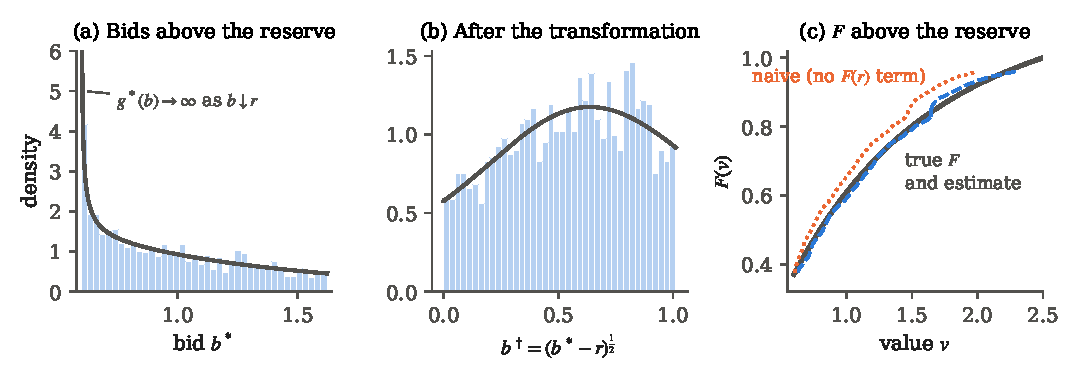
\includegraphics[width=\textwidth]{figures/ch15/gpv_reserve.pdf}
\caption{A binding reserve price. $T=500$ auctions with $N=5$ potential bidders, values lognormal$(0,1)$ truncated to $[0.055,2.5]$, reserve price $r=0.6$ with $F(r)=0.370$. Panel (a): histogram of the 1,627 actual bids and the true density $g^*$, which diverges at $r$. Panel (b): the transformed bids $(b^*-r)^{\frac12}$ have a bounded density. Panel (c): true $F$ above $r$ (solid), the estimate based on \eqref{eq:15-gpv-reserve-dagger} with $\hat N=5$ and $\hat F(r)=0.349$ (dashed), and a naive estimate that drops the term in $F(r)$ (dotted). Our simulation (seed 15404).}\label{fig:15-gpv-reserve}
\end{figure}

\Cref{fig:15-gpv-reserve} applies the procedure to simulated data. With $N=5$ and $r=0.6$, the expected number of actual bidders is $5(1-0.370)=3.15$. In the sample, $\hat N=5$ and $\hat F(r)=1-\frac{3.254}{5}=0.349$. The design has no covariates, and the estimates of $G^\dagger$ and $g^\dagger$ pool all 1,627 actual bids. The one auction of the 500 without a bid therefore enters only $\hat F(r)$. Among bids that survive trimming, the mean absolute error of the pseudo-values is 0.025 with the full formula and 0.151 for the naive formula without the term in $F(r)$. For values within 0.3 of the reserve, the naive pseudo-values are too low by 0.078 on average. The missing term is the markdown that comes from competing against potential bidders who stay out.

\casehead{Affiliated values and observed participation} \Citet[Section 6.3.1]{AtheyHaile2007} extend these results to affiliated private values when bidders do not know the set of actual bidders. With all bids, bidder identities and the reserve price, the joint distribution of the actual bidders' values above $r$ is identified (their Theorem 6.4). Each marginal $F_i$ is identified above $r$ when the set of potential bidders is observed (their Theorem 6.5). \Cref{sec:15-entry-reserve} states these results and the inversion behind them. Exogenous variation in reserve prices would trace out more of $F$, as GPV note. Estimators that combine auctions with different reserve prices to recover $F$ below the observed reserves had not been developed when Athey and Haile wrote their survey \citep[Section 6.3.1]{AtheyHaile2007}. \Cref{sec:15-uh} discusses the opposite case, in which the reserve price carries information about the object.

\subsection{Incomplete bid data and Dutch auctions}\label{sec:15-gpv-winbid}

Many data sets record only the winning bid. In a Dutch auction the clock stops at the first bid, so only the transaction price exists. The Dutch auction is strategically equivalent to the first-price auction (\cref{prop:14-dutch-fpa}). In other settings the auctioneer records only the winner. With independent private values, the winning bid suffices.

\begin{proposition}[\citealp{AtheyHaile2002}, Theorem 6(i), and \citealp{AtheyHaile2007}, Theorem 3.2 and Corollary 3.1]\label{prop:15-winbid}
In a first-price or Dutch auction with independent private values, suppose the transaction price and the number of bidders are observed. If bidders are asymmetric, suppose also that the set of bidders and the identity of the winner are observed. Then the value distribution of every bidder is identified.
\end{proposition}

\begin{proof}
\emph{Symmetric bidders.} Let $G_{(n:n)}$ denote the distribution of the winning bid $B^{(n:n)}$, with density $g_{(n:n)}$. Bids are i.i.d.\ with distribution $G$, so $G_{(n:n)}(b)=G(b)^n$ and
\begin{equation}\label{eq:15-winbid-G}
G(b)=G_{(n:n)}(b)^{\frac1n}.
\end{equation}
Hence the winning bid identifies the distribution of a single bid, and \cref{thm:15-gpv-ident} applies. To write the inverse bid function directly in terms of the winning bid, differentiate: $g_{(n:n)}(b)=nG(b)^{n-1}g(b)$. Then
\[
\frac{G_{(n:n)}(b)}{g_{(n:n)}(b)}=\frac{G(b)^n}{nG(b)^{n-1}g(b)}=\frac{G(b)}{ng(b)}=\frac{n-1}{n}\cdot\frac{G(b)}{(n-1)g(b)},
\]
which is equation (3.7) of \citet{AtheyHaile2007}. Substituting into \eqref{eq:15-gpv-xi},
\begin{equation}\label{eq:15-winbid-xi}
\xi(b)=b+\frac{n}{n-1}\,\frac{G_{(n:n)}(b)}{g_{(n:n)}(b)}.
\end{equation}
This observation is due to \citet{GuerrePerrigneVuong1995}.

\emph{Asymmetric bidders.} Let $G_i$ denote the distribution of bidder $i$'s bid, and let $G^w_i(b)=\Pr(B_i\le b,\ B_i\ge B_j\text{ for all }j)$ be the probability that $i$ wins with a bid of at most $b$. It is observable when the winner's identity is recorded. By independence,
\[
G^w_i(b)=\int_{\underline b}^b\prod_{j\neq i}G_j(s)\,dG_i(s).
\]
Summing over bidders, $\sum_jG^w_j(s)=\Pr(\max_jB_j\le s)=\prod_jG_j(s)$, the distribution of the winning bid. Therefore
\[
\frac{dG^w_i(s)}{\sum_jG^w_j(s)}=\frac{\prod_{j\neq i}G_j(s)\,dG_i(s)}{\prod_jG_j(s)}=\frac{dG_i(s)}{G_i(s)}=d\ln G_i(s).
\]
Integrating from $b$ to $\bar b$ and using $G_i(\bar b)=1$ gives
\begin{equation}\label{eq:15-berman}
G_i(b)=\exp\Big\{-\int_b^{\bar b}\Big(\sum_{j=1}^nG^w_j(s)\Big)^{-1}dG^w_i(s)\Big\}.
\end{equation}
This is the competing-risks formula of \citet{Berman1963}, adapted to auctions by \citet{AtheyHaile2002}. The right side is observable, so each $G_i$ is identified. The marginals $G_j$ determine the distribution of each bidder's highest rival bid, $G_{M_i}=\prod_{j\neq i}G_j$. The asymmetric first-order condition \eqref{eq:14-asym-foc}, rearranged as $v_i=b+\big[\sum_{j\neq i}\frac{g_j(b)}{G_j(b)}\big]^{-1}$, then gives each inverse bid function and each $F_i$.
\end{proof}

The formula in \citet[eq.~(3.8)]{AtheyHaile2007} is printed with the integral running from $-\infty$ to $b$ and without the minus sign. The derivation above gives the form \eqref{eq:15-berman}. \Citet{BrendstrupPaarsch2003} propose estimating \eqref{eq:15-berman} by replacing $G^w_i$ with its empirical counterpart and $dG^w_i$ with a kernel estimate \citep[Section 3.3.1]{AtheyHaile2007}. Athey and Haile add that survival-analysis estimators such as the Kaplan-Meier or Nelson-Aalen estimators could be adapted.

\casehead{Estimation with symmetric bidders} With $T$ winning bids $B^w_t$, one estimates $G_{(n:n)}$ by the empirical distribution and $g_{(n:n)}$ by a kernel estimator. Equation \eqref{eq:15-winbid-xi} then gives the estimated winner's value $\hat V^{(n:n)}_t=\hat\xi(B^w_t)$, after trimming as in \eqref{eq:15-gpv-trim}. The winners' values have distribution $F^n$, so $\hat F(v)=\big[\frac1T\sum_t\indic(\hat V^{(n:n)}_t\le v)\big]^{\frac1n}$.

\casehead{The cost of observing only the winner} The data contain one bid per auction instead of $n$, and the inversion through the $n$-th root loses precision in the lower tail. To see how much, ignore first-step error and suppose the winners' values were observed. Let $H=F^n$ and let $\hat H$ be the empirical distribution of the $T$ winners' values, with variance $\frac{H(1-H)}{T}$. Since $\frac{dF}{dH}=\frac1nH^{\frac1n-1}=\frac1nF^{1-n}$, the delta method gives
\[
\Var\big(\hat F(v)\big)\approx\frac{1}{n^2}F^{2-2n}\,\frac{F^n(1-F^n)}{T}=\frac{F^{2-n}(1-F^n)}{n^2T}.
\]
With all $nT$ values observed, the variance of the empirical distribution is $\frac{F(1-F)}{nT}$. The ratio of the two variances is
\[
\frac{F^{2-n}(1-F^n)}{n^2T}\cdot\frac{nT}{F(1-F)}=\frac{1-F^n}{nF^{n-1}(1-F)}=\frac{1+F+\dots+F^{n-1}}{nF^{n-1}}.
\]
It equals one at the top of the support and grows without bound as $F\to0$. With $n=5$ at the median of $F$, the ratio is $\frac{1.9375}{0.3125}=6.2$. This is our calculation. The winning bid identifies $F$, but low values are rarely revealed by winners, so the lower tail is estimated poorly.

\casehead{An unknown number of bidders} In some Dutch auctions only the transaction price is recorded, and the number of bidders is unknown. Then $F$ is not identified nonparametrically \citep[Section 3.3.1]{AtheyHaile2007}. For any candidate $n'$, the distribution $G_{(n:n)}^{\frac{1}{n'}}$ is a valid bid distribution, and $n'$ bidders bidding i.i.d.\ from it generate the same winning-bid distribution. Each $n'$ for which the implied inverse bid function is increasing yields a different $F$. \Citet{LaffontOssardVuong1995} instead estimate $n$ within a parametric model (\cref{sec:15-direct}).

\casehead{Covariates and testability} \Citet[Theorem 6]{AtheyHaile2002} extend the result in three directions. If $V_i=g_i(A_i,W_0)$ with $W_0$ observed by bidders and the econometrician and $A_1,\dots,A_n$ independent given $W_0$, then each $F_i(\cdot\mid w_0)$ is identified, because part (i) applies for each fixed $w_0$. If $V_i=g_0(W_0)+A_i$ with the $A_i$ mutually independent and independent of $W_0$, then each $F_{A_i}$ and $g_0$ are identified up to location. Finally, the models are testable. With symmetric bidders, observing more than one bid per auction, or exogenous variation in $n$, gives two estimates of $G$ from \eqref{eq:15-winbid-G} that must agree. With asymmetric bidders, observing the second-highest bid or exogenous variation in $n$ plays the same role \citep[Theorem 6(iv)--(v)]{AtheyHaile2002}.

\subsection{Specification testing in first-price auctions}\label{sec:15-gpv-tests}

\Cref{thm:15-gpv-ident} lists the restrictions that the SIPV model places on bids. \Citet[Section 5.1]{AtheyHaile2007} characterize the restrictions in the broader affiliated private values (APV) model of \cref{sec:15-apv}. Write $\xi_i(b;\mathcal N)=b+\frac{G_{M_i\mid B_i}(b\mid b;\mathcal N)}{g_{M_i\mid B_i}(b\mid b;\mathcal N)}$ for bidder $i$'s inverse bid function when the set of bidders is $\mathcal N$. Here $M_i$ is the highest rival bid and $G_{M_i\mid B_i}$ its distribution conditional on $i$'s bid, as in \eqref{eq:15-lpv-foc}. Let $[\underline b_i,\bar b_i]$ be the support of $B_i$.

\begin{theorem}[\citealp{AtheyHaile2007}, Theorem 5.2]\label{thm:15-ah-rational}
Consider the APV first-price auction with a fixed set of bidders $\mathcal N$. Assume the joint density of values is continuously differentiable, and that either (i) values are mutually independent or (ii) bidders are symmetric. A joint distribution of bids $\mathbf G$ is rationalized by equilibrium bidding if and only if:
\begin{itemize}
\item[(a)] The bids $(B_1,\dots,B_n)$ are affiliated. They are independent in case (i) and exchangeable in case (ii).
\item[(b)] Each $\xi_i(\cdot;\mathcal N)$ is differentiable and strictly increasing on the support of $B_i$.
\item[(c)] The distribution $\mathbf G\big(\xi_1^{-1}(u_1;\mathcal N),\dots,\xi_n^{-1}(u_n;\mathcal N)\big)$ is absolutely continuous in $\bm u$. Its density is positive and continuously differentiable on the product of the supports of $\xi_i(B_i;\mathcal N)$ and zero elsewhere.
\item[(d)] $\xi_i(\underline b;\mathcal N)=\underline b$ for all $i$.
\item[(e)] $\xi_i(\bar b_i;\mathcal N)=\xi_j(\bar b_j;\mathcal N)$ for all $i,j$.
\item[(f)] The support of $B_i$ is convex, compact, and the same for all $i$.
\end{itemize}
\end{theorem}

Without independence or symmetry, conditions of this type remain necessary but are not known to be sufficient. The equilibrium of the asymmetric APV model lacks a full characterization \citep[Theorem 5.1]{AtheyHaile2007}. Sufficiency in \cref{thm:15-ah-rational} uses the argument of Step 4 in the proof of \cref{thm:15-gpv-ident}. Under independence or symmetry, payoffs satisfy single crossing. Local optimality of each bid together with monotone strategies then implies global optimality. Athey and Haile stress why such a result matters. Without it, nothing guarantees that a bid $b$ is a best response for the value $\xi_i(b)$ that the first-order condition assigns to it. Verifying the conditions is the analog of verifying second-order conditions \citep[Section 5.1]{AtheyHaile2007}. For SIPV, the conditions reduce to (C1)--(C2) of \cref{thm:15-gpv-ident}.

Each condition suggests a test. We describe the main ones, following \citet[Sections 5.2--5.5]{AtheyHaile2007}.

\casehead{Monotonicity of the inverse bid function} Condition (C2), or (b), says that $\hat\xi$ should be increasing. GPV propose this as a test of equilibrium bidding and note that it requires estimating $\xi$ under a monotonicity constraint \citep[p.~552]{GuerrePerrigneVuong2000}. No formal test had been developed by the time of the Athey-Haile survey. Standard tests of monotone regression do not apply directly, because the realizations $\xi_i(B_i)$ are themselves estimates. Applications typically find few violations \citep{HendricksPinksePorter2003,HaileHongShum2003}. Two caveats apply. First, a rejection does not reveal which assumption failed: unobserved heterogeneity, risk aversion, or non-equilibrium play could each cause it. Second, no test of monotonicity is consistent against all violations of the model, since some misspecified models still produce an increasing $\xi$.

\casehead{The boundary condition} Condition (e) says that all bidders' inverse bid functions meet at the top of the bid support, since all bidders share the upper bound of values. In the asymmetric IPV model, $G_{M_i}(\bar b)=1$, so $\xi_i(\bar b)=\bar b+\frac{1}{g_{M_i}(\bar b)}$, and (e) becomes
\begin{equation}\label{eq:15-boundary-test}
g_{M_i}(\bar b)=g_{M_j}(\bar b)\qquad\text{for all }i,j,
\end{equation}
which is equation (5.1) of \citet{AtheyHaile2007}. The densities of the highest rival bid must agree at the top. \Cref{sec:15-apv-asym} works through an example of Athey and Haile in which the condition fails because the value supports of the two bidders have different upper bounds, which the maintained model excludes.

\casehead{Multi-sample tests with exogenous variation in $n$} If the number of bidders varies exogenously, the value distribution estimated from $n$-bidder auctions must equal the one estimated from $n'$-bidder auctions. Under IPV, the inverse bid functions $\xi(\cdot;G_n,n)$ differ across $n$, because bidding becomes more aggressive as $n$ rises (\cref{prop:14-fpa-n}). The implied value distributions must nevertheless coincide. Testing equality of distributions is standard when the data are observed. Here the values are estimated in a first nonparametric step, which complicates the asymptotic theory. \Citet{HaileHongShum2003} develop formal tests of this kind. They use them to test private against common values, which \cref{sec:15-cv} takes up.

\casehead{Multiple order statistics} In IPV models, any single order statistic of bids identifies $F$, together with $n$. When two order statistics are recorded, for example the two highest bids, the two implied estimates of $F$ must agree up to sampling error. This test needs no variation in $n$ \citep[Section 5.4]{AtheyHaile2007}.

\casehead{Direct tests of independence and exchangeability} Condition (C1) can be tested directly when all bids are observed. Exchangeability can be tested with the bootstrap distance tests of \citet{Romano1988,Romano1989}, which compare a multivariate distribution with its permutations. Equality of the marginal distributions of different bidders can be tested by Kolmogorov-Smirnov statistics. Independence can be tested by comparing the joint distribution of bids with the product of its marginals. GPV suggest the test of \citet{BlumKieferRosenblatt1961}, which \citet{CampoPerrigneVuong2003} later apply to offshore oil bids. With covariates, regression tests of conditional independence and exchangeability are natural. \Cref{sec:15-collusion} describes them in the form that \citet{BajariYe2003} use to look for collusion in highway procurement.

\citet[p.~2123]{AtheyHaile2002} add a warning. Monotonicity of $\xi$ holds under many natural alternatives to the IPV model, so the test most often used in early work has little power against affiliated or common values. The restrictions that come from comparing different order statistics or different numbers of bidders typically fail under those alternatives. They are the more informative tests.

\casehead{Assessment} GPV changed the econometrics of auctions. Before them, structural work required closed-form equilibria or simulation, and parametric assumptions carried an unclear part of the identification \citep[Section 3.1]{AtheyHaile2007}. After them, the first-order condition became a measurement device. The ingredients were a constructive identification result with sharp testable restrictions, an estimator that requires only kernel smoothing, and a proof that the estimator is rate-optimal. The same principle extends to affiliated values, asymmetric bidders, procurement with quality, binding reserve prices and dynamic bidding. It also inspired parametric two-step estimators that keep the inversion and add structure in one of the steps \citep[footnote 25]{GuerrePerrigneVuong2000}.

The approach has limits that later sections address. It maintains independent private values and risk neutrality, and it assumes that observed covariates capture all heterogeneity across auctions. Ignoring unobserved heterogeneity flattens the estimated inverse bid function and inflates estimated markups (\cref{sec:15-uh}). The second step pools across $n$ only if participation is exogenous given covariates (\cref{sec:15-entry}). Each additional continuous covariate slows convergence, and the boundary trimming discards the tails of $F$, which matter for reserve prices. No distribution theory for $\hat f$ was available. Bandwidth constants are set by rules of thumb, and data-driven choices had not been explored \citep[Section 3.2.1]{AtheyHaile2007}. Finally, the model needs all bids, or the winning bid with known $n$. When bidding takes place under richer information structures, bids reveal less, as \cref{sec:15-apv,sec:15-cv} show.

The rest of the chapter relaxes the maintained assumptions one at a time. \Cref{sec:15-apv} replaces independence with affiliation and symmetry with bidder classes, and the inversion runs through the distribution of the highest rival bid conditional on one's own bid. \Cref{sec:15-cv} asks what bids can reveal when values are common. \Cref{sec:15-uh} handles heterogeneity that bidders observe and the econometrician does not. \Cref{sec:15-entry} treats endogenous participation, dynamics and risk aversion. In each case the first step of the GPV estimator survives, and the work lies in finding the right conditioning set for the distribution of rival bids.

\section{Affiliated and Asymmetric Private Values}\label{sec:15-apv}

The inversion of \cref{sec:15-gpv} rests on two assumptions besides private values. Values are
independent across bidders, and bidders are symmetric. Both assumptions often fail. Bidders who appraise
the same tract of timber tend to have correlated values. They react to features of the tract that the
econometrician does not record. Bidders also differ in systematic ways. A sawmill differs from a logger,
a consortium from a single firm, and a contractor next to the site from one far away.

This section shows that the first-order condition can still be inverted when both assumptions fail. The
key observable becomes the joint distribution of a bidder's own bid and the highest rival bid. We first
treat symmetric affiliated private values \citep{LiPerrigneVuong2002}. We then ask what the two highest
bids alone reveal \citep{AtheyHaile2002}. Next we study asymmetric affiliated private values and joint
bidding for offshore oil leases \citep{CampoPerrigneVuong2003}. We close with asymmetric independent
private values.

\subsection{Symmetric affiliated private values: Li, Perrigne and Vuong (2002)}\label{sec:15-apv-lpv}

\casehead{Question} Before 2002, structural work on first-price auctions used either the independent
private value (IPV) model or the pure common value model. \citet{LiPerrigneVuong2002}, henceforth LPV, ask whether the
\emph{affiliated private value} (APV) model can be identified and estimated from bids alone, without a
parametric form for the dependence among values. The question matters because affiliation changes
equilibrium shading. An analyst who imposes independence on affiliated data misreads bids, and so
misreads values and rents.

\casehead{Model} A single object is sold by first-price sealed bid to $n\ge2$ risk-neutral bidders. In the
affiliated value model of \citet{MilgromWeber1982}, bidder $i$'s utility is $U(v_i,c)$, where $v_i$ is
her private signal and $c$ a common component. The APV model is the case $U(v,c)=v$. Values
$\bm V=(V_1,\dots,V_n)$ have a joint distribution $F$ with density $f$ on $[\underline v,\bar v]^n$. The
density is symmetric (exchangeable) and affiliated in the sense of \cref{def:14-affiliation}. The reserve
price does not bind. Let $Y_1=\max_{j\ne1}V_j$ be the highest rival value. Write $F_{Y_1\mid V_1}$ and
$f_{Y_1\mid V_1}$ for its conditional distribution and density given $V_1$. Affiliation leaves the form of
dependence unrestricted. A common component plus independent noise is one example among many.

The symmetric equilibrium in strictly increasing strategies $\beta$ is the special case of
\cref{prop:14-mw-fpa} with $v(\alpha,\alpha)=\alpha$. It solves the differential equation
\begin{equation}\label{eq:15-lpv-ode}
  \beta'(v)=\bigl(v-\beta(v)\bigr)\frac{f_{Y_1\mid V_1}(v\mid v)}{F_{Y_1\mid V_1}(v\mid v)},
  \qquad \beta(\underline v)=\underline v,
\end{equation}
which is equation (1) of \citet{LiPerrigneVuong2002}. Its solution is
\begin{equation}\label{eq:15-lpv-bid}
  \beta(v)=v-\int_{\underline v}^{v}L(\alpha\mid v)\,d\alpha,
  \qquad
  L(\alpha\mid v)=\exp\left(-\int_\alpha^v\frac{f_{Y_1\mid V_1}(u\mid u)}{F_{Y_1\mid V_1}(u\mid u)}\,du\right),
\end{equation}
their equation (2). The bid depends on $F$ through the whole conditional law of the highest rival value
along the diagonal. A parametric family for $F$, such as a multivariate lognormal, rarely yields a closed
form for $\beta$.

\casehead{From the differential equation to observables} Bids are random with joint distribution
$\bm G$, which the econometrician observes when all bids are recorded. Let $B_i$ be bidder $i$'s bid and
$M_i=\max_{j\ne i}B_j$ the highest rival bid. Let $G_{M\mid B}(m\mid b)=\Pr(M_i\le m\mid B_i=b)$, with
density $g_{M\mid B}(m\mid b)$ in $m$. Because $\beta$ is strictly increasing, $M_1=\beta(Y_1)$ and the
event $\{B_1=b\}$ equals $\{V_1=\beta^{-1}(b)\}$. Hence
\begin{align*}
  G_{M\mid B}(m\mid b)&=\Pr\bigl(\beta(Y_1)\le m\mid \beta(V_1)=b\bigr)
  =F_{Y_1\mid V_1}\bigl(\beta^{-1}(m)\mid\beta^{-1}(b)\bigr),\\
  g_{M\mid B}(m\mid b)&=\frac{f_{Y_1\mid V_1}\bigl(\beta^{-1}(m)\mid\beta^{-1}(b)\bigr)}{\beta'\bigl(\beta^{-1}(m)\bigr)}.
\end{align*}
Evaluate both at $m=b=\beta(v)$ and take the ratio:
\begin{equation*}
  \frac{G_{M\mid B}(b\mid b)}{g_{M\mid B}(b\mid b)}
  =\beta'(v)\,\frac{F_{Y_1\mid V_1}(v\mid v)}{f_{Y_1\mid V_1}(v\mid v)}
  =v-\beta(v),
\end{equation*}
where the second equality is \eqref{eq:15-lpv-ode}. Rearranging gives the inverse bid function
\begin{equation}\label{eq:15-lpv-foc}
  v=\xi(b;\bm G)\equiv b+\frac{G_{M\mid B}(b\mid b)}{g_{M\mid B}(b\mid b)},
\end{equation}
equation (4) of \citet{LiPerrigneVuong2002}. It is the first-order condition \eqref{eq:14-apv-foc}
written in observables. Conditioning on the value is the same as conditioning on the bid, because the
equilibrium is strictly monotone. With independent values $G_{M\mid B}(b\mid b)=G(b)^{n-1}$, and
\eqref{eq:15-lpv-foc} reduces to the inversion \eqref{eq:15-gpv-xi}.

\begin{definition}[Rationalization in the APV model]\label{def:15-lpv-rational}
A joint distribution $\bm G$ of bids is \emph{rationalized} by an APV structure $F$ if $\bm G$ is the
equilibrium bid distribution of the first-price auction with values drawn from $F$. The APV model is
identified if no two distinct structures $F\ne\tilde F$ lead to the same $\bm G$
\citep[Definition~1]{LiPerrigneVuong2002}.
\end{definition}

\begin{proposition}[{\citealp[Proposition~1]{LiPerrigneVuong2002}}]\label{prop:15-lpv}
The symmetric APV model is identified. Let $\bm G$ have support $[\underline b,\bar b]^n$. It can be
rationalized by a symmetric APV model if and only if two conditions hold.
\begin{enumerate}[label=(\roman*)]
  \item $\bm G$ is symmetric and affiliated.
  \item $\xi(\cdot;\bm G)$ in \eqref{eq:15-lpv-foc} is strictly increasing on $[\underline b,\bar b]$.
\end{enumerate}
The sufficiency direction also maintains the boundary condition
$\frac{G_{M\mid B}(b\mid b)}{g_{M\mid B}(b\mid b)}\to0$ as $b\downarrow\underline b$, which every rationalizable $\bm G$
satisfies. The rationalizing distribution is
\begin{equation}\label{eq:15-lpv-F}
  F(v_1,\dots,v_n)=\bm G\bigl(\xi^{-1}(v_1;\bm G),\dots,\xi^{-1}(v_n;\bm G)\bigr).
\end{equation}
\end{proposition}

\begin{proof}
\emph{Identification.} Let $F$ and $\tilde F$ both generate $\bm G$, with equilibrium strategies $\beta$ and
$\tilde\beta$. Both strategies satisfy \eqref{eq:15-lpv-ode}, which is equivalent to
\eqref{eq:15-lpv-foc}. So $\beta^{-1}=\tilde\beta^{-1}=\xi(\cdot;\bm G)$, and
$F(\bm v)=\Pr\bigl(\xi(B_i)\le v_i\ \forall i\bigr)=\tilde F(\bm v)$.

\emph{Necessity.} If $F$ rationalizes $\bm G$, then $\bm G(\bm b)=F\bigl(\beta^{-1}(b_1),\dots,\beta^{-1}(b_n)\bigr)$.
Strictly increasing transformations preserve symmetry and affiliation, which gives (i). Since
$\xi=\beta^{-1}$, (ii) holds. The ratio in the boundary condition equals $\xi(b)-b=\beta^{-1}(b)-b$, which tends to
zero as $b\downarrow\underline b$ because $\beta(\underline v)=\underline v$.

\emph{Sufficiency.} Let $\bm G$ satisfy (i) and (ii) and define $F$ by \eqref{eq:15-lpv-F}. Then $F$ is a
symmetric affiliated distribution on $[\underline v,\bar v]^n$ with
$\underline v=\xi(\underline b)$ and $\bar v=\xi(\bar b)$. Let bidders use $\beta=\xi^{-1}$. Then
$\bm G=F\circ\beta^{-1}$ by construction, and the steps above reverse to show that $\beta$ solves
\eqref{eq:15-lpv-ode}. For the boundary condition, LPV argue that $\ln G_{M\mid B}$ diverges at
$\underline b$. Divergence of the logarithm alone does not force the markdown
$\frac{G_{M\mid B}(b\mid b)}{g_{M\mid B}(b\mid b)}$ to vanish. This is why the proposition maintains
that this ratio tends to zero as $b\downarrow\underline b$. A bid density bounded away from zero at $\underline b$ is
sufficient but too strong. With i.i.d.\ uniform values and $n\ge3$ the density tends to zero, yet the ratio
equals $\frac{b}{n-1}$ and still vanishes. Under the maintained condition, $\xi(\underline b)=\underline b$, so
$\beta(\underline v)=\underline v$.
Second-order conditions are maintained throughout \citep[footnote~7]{LiPerrigneVuong2002}.
\end{proof}

Three remarks place the result. First, \citet{LaffontVuong1996} show that the general affiliated value
model is not identified from bids. Any affiliated value model with fixed $n$ is observationally equivalent
to some APV model. Restricting attention to APV therefore loses nothing in explaining bids. In this
sense the symmetric APV model is the most general model identified from bids alone
\citep[p.~175]{LiPerrigneVuong2002}. It does not exclude common values. It only cannot distinguish them
(\cref{sec:15-cv-limits}). Second, condition (ii) is a testable restriction of equilibrium play, as in
\cref{thm:15-gpv-ident}. Third, condition (i) implies that independence of values can be tested through
independence of bids within auctions, for example with the test of \citet{BlumKieferRosenblatt1961}.

\casehead{Estimator} The ratio in \eqref{eq:15-lpv-foc} can be written with joint objects that are easier to
estimate. Let $G_{M,B}(m,b)=G_{M\mid B}(m\mid b)\,g_B(b)$, which is $\frac{\partial}{\partial b}\Pr(M\le
m,\,B\le b)$, and let $g_{M,B}(m,b)=g_{M\mid B}(m\mid b)\,g_B(b)$ be the joint density of $(M,B)$. Then
\begin{equation*}
  \frac{G_{M\mid B}(b\mid b)}{g_{M\mid B}(b\mid b)}
  =\frac{G_{M\mid B}(b\mid b)\,g_B(b)}{g_{M\mid B}(b\mid b)\,g_B(b)}
  =\frac{G_{M,B}(b,b)}{g_{M,B}(b,b)},
\end{equation*}
because the marginal density $g_B$ cancels. Fix $n$ and let $T_n$ be the number of $n$-bidder auctions.
With a kernel $\mathcal K$ and bandwidths $h_G$ and $h_g$, the first step computes
\begin{align}
  \hat G_{M,B}(b,b)&=\frac{1}{nT_nh_G}\sum_{t=1}^{T_n}\sum_{i=1}^{n}\indic(M_{it}\le b)\,
  \mathcal K\left(\frac{b-B_{it}}{h_G}\right),\label{eq:15-lpv-Ghat}\\
  \hat g_{M,B}(b,b)&=\frac{1}{nT_nh_g^2}\sum_{t=1}^{T_n}\sum_{i=1}^{n}
  \mathcal K\left(\frac{b-M_{it}}{h_g}\right)\mathcal K\left(\frac{b-B_{it}}{h_g}\right),\label{eq:15-lpv-ghat}
\end{align}
equations (5)--(6) of \citet{LiPerrigneVuong2002} and (3.3)--(3.4) of \citet{AtheyHaile2007}. Averaging over
the $n$ bidders in each auction uses symmetry. The pseudo-values are
\begin{equation}\label{eq:15-lpv-pseudo}
  \hat V_{it}=B_{it}+\frac{\hat G_{M,B}(B_{it},B_{it})}{\hat g_{M,B}(B_{it},B_{it})}
  \quad\text{if } B_{\min}+h_g\le B_{it}\le B_{\max}-h_g,
\end{equation}
and $\hat V_{it}=+\infty$ otherwise. Trimming bids within one bandwidth of the boundaries removes the
pseudo-values that kernel boundary bias would distort \citep[p.~181]{LiPerrigneVuong2002}.

The second step estimates the $n$-variate density of values from the auctions that survive trimming,
\begin{equation}\label{eq:15-lpv-fhat}
  \hat f(v_1,\dots,v_n)=\frac{1}{T_nh_f^n}\sum_{t=1}^{T_n}
  \mathcal K_f\left(\frac{v_1-\hat V_{1t}}{h_f},\dots,\frac{v_n-\hat V_{nt}}{h_f}\right),
\end{equation}
with a product kernel $\mathcal K_f$. A kernel with compact support gives zero weight to any auction with
an infinite pseudo-value, so trimmed auctions drop out. Symmetry is imposed by averaging $\hat f$ over the
$n!$ permutations of its arguments. The marginal density of values uses all pseudo-values,
$\hat f_n(v)=\frac{1}{nT_nh_m}\sum_t\sum_i\mathcal K\bigl(\frac{v-\hat V_{it}}{h_m}\bigr)$. Comparing
$\hat f_n$ across $n$ checks whether the value distribution depends on the number of bidders. If it does
not, pseudo-values from different $n$ can be pooled.

\begin{remark}[Rates]\label{rem:15-lpv-rates}
Let $f$ have $R$ continuous bounded derivatives. With $h_G\propto(\frac{\log T_n}{T_n})^{\frac{1}{2R+2n-3}}$,
$h_g\propto(\frac{\log T_n}{T_n})^{\frac{1}{2R+2n-2}}$ and
$h_f\propto(\frac{\log T_n}{T_n})^{\frac{R+n-2}{(R+n+1)(2R+2n-2)}}$, and if $R>n-2$, $\hat f$ is uniformly
consistent on inner compact sets with rate $(\frac{T_n}{\log T_n})^{\frac{R(R+n-2)}{(R+n+1)(2R+2n-2)}}$
\citep[Proposition~2]{LiPerrigneVuong2002}. With observed values the optimal rate would be
$(\frac{T_n}{\log T_n})^{\frac{R}{2R+n}}$ \citep{Stone1982}. For $R=2$ and $n=2$ the exponents are
$\frac{2}{15}$ and $\frac{5}{15}$. The marginal density $\hat f_n$ converges faster, with exponent
$\frac{(R+n-1)(R+n-2)}{(R+n+1)(2R+2n-2)}$ \citep[Proposition~3]{LiPerrigneVuong2002}, which equals
$\frac15$ for $R=2$ and $n=2$. Optimality of these rates is not established, because the minimax argument of
\citet{GuerrePerrigneVuong2000} does not carry over. The exponents fall with $n$. This is the curse of
dimensionality.
\end{remark}

\casehead{Implementation} \citet[pp.~180--181]{LiPerrigneVuong2002} use the triweight kernel
$\mathcal K(u)=\frac{35}{32}(1-u^2)^3\indic(|u|\le1)$, a kernel of order two, and product kernels in several
dimensions. Kernels of order three would be required in theory for $n=3$. They would produce negative
density estimates and pseudo-values below bids, so order two is used throughout. Bandwidths follow the
rate in \cref{rem:15-lpv-rates} with $R=2$. For $n=2$ they set $h_G=c_G(nT)^{-\frac15}$ and
$h_g=c_g(nT)^{-\frac16}$. For $n=3$ the exponents are $-\frac17$ and $-\frac18$. The constants follow
Silverman's rule of thumb, $c=2.978\times1.06\,\hat\sigma_b$, where $\hat\sigma_b$ is the standard
deviation of bids. The factor $2.978$ converts the rule from a Gaussian to a triweight kernel. In the second
step $h_f=c_f(2!\,T^\ast)^{-\frac{1}{15}}$ for $n=2$ and $c_f(3!\,T^\ast)^{-\frac{1}{16}}$ for $n=3$, with
$T^\ast$ the number of auctions left after trimming. When bids are skewed, the authors suggest working with
$\ln(1+b)$ and transforming back \citep[footnote~13]{LiPerrigneVuong2002}.

\casehead{Monte Carlo design} The design follows the laboratory experiments of
\citet{KagelHarstadLevin1987}. Each value is a common draw plus noise, $V_i=Q+E_i$, with $Q$ uniform on
$[\frac14,\frac34]$ and $E_i$ independent and uniform on $[-\frac14,\frac14]$. Values lie in $[0,1]$. Since
$\Var(Q)=\Var(E_i)=\frac{1}{48}$, the correlation between two values is
\begin{equation*}
  \Corr(V_i,V_j)=\frac{\Var(Q)}{\Var(Q)+\Var(E_i)}=\frac12 .
\end{equation*}
The sum of two independent uniforms of width $\frac12$ has the triangular marginal density
$f(v)=4v$ on $[0,\frac12]$ and $f(v)=4-4v$ on $[\frac12,1]$. Its kink at $\frac12$ makes it
nondifferentiable there.

We can derive the equilibrium for $v\le\frac12$ by hand. Given $V_1=v\le\frac12$, Bayes' rule makes $Q$
uniform on $[\frac14,v+\frac14]$. Given $Q=q$, each rival value is below $x$ with probability
$2(x-q)+\frac12$, clipped to $[0,1]$. For $x\le v$ the substitution $u=2(x-q)+\frac12$ gives
\begin{equation*}
  F_{Y_1\mid V_1}(x\mid v)=\frac1v\int_{\frac14}^{x+\frac14}\Bigl(2(x-q)+\frac12\Bigr)^{n-1}dq
  =\frac{1}{2v}\int_0^{2x}u^{n-1}\,du=\frac{(2x)^n}{2nv}.
\end{equation*}
For $x$ slightly above $v$ the upper limit of $q$ is $v+\frac14$, so
$F_{Y_1\mid V_1}(x\mid v)=\frac{(2x)^n-(2x-2v)^n}{2nv}$. Both pieces have derivative $2^{n-1}v^{n-2}$ at
$x=v$, and $F_{Y_1\mid V_1}(v\mid v)=\frac{2^{n-1}v^{n-1}}{n}$. Therefore
\begin{equation*}
  \frac{f_{Y_1\mid V_1}(v\mid v)}{F_{Y_1\mid V_1}(v\mid v)}=\frac nv,
  \qquad
  \beta'(v)=\bigl(v-\beta(v)\bigr)\frac nv .
\end{equation*}
The linear function $\beta(v)=\frac{n}{n+1}v$ satisfies this equation and $\beta(0)=0$. This is equation (10)
of \citet{LiPerrigneVuong2002}. For $n=2$ the same line $\beta(v)=\frac23v$ holds on all of $[0,1]$
(their equation (11)). For $n=3$ the bid is nonlinear above $\frac12$ (their equation (12)). A simple
design thus produces a complicated equilibrium.

Compare the IPV benchmark with the same triangular marginal. On $[0,\frac12]$, $F(v)=2v^2$, and the
bid of \eqref{eq:14-rs-bid} is
\begin{equation*}
  \beta^{IPV}(v)=v-\frac{\int_0^v(2x^2)^{n-1}dx}{(2v^2)^{n-1}}=v-\frac{v}{2n-1}=\frac{2n-2}{2n-1}\,v .
\end{equation*}
For $n=2$ this equals the APV bid $\frac23v$. For $n=3$ it is $\frac45v$, above the APV bid $\frac34v$
\citep[footnote~17]{LiPerrigneVuong2002}. \Cref{fig:15-lpv-design} shows both strategies on the whole
support. Affiliation makes low types bid less aggressively and high types more aggressively. A bidder with a
low value expects rivals with low values, so she faces weak competition. A bidder with a high value expects
strong competition and shades less.

\begin{figure}[htbp]
  \centering
  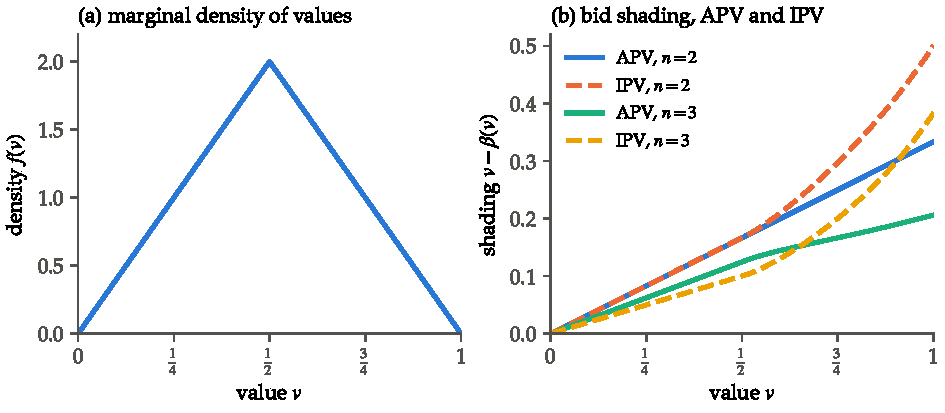
\includegraphics[width=\textwidth]{figures/ch15/lpv_design.pdf}
  \caption{The Monte Carlo design of \citet{LiPerrigneVuong2002}. Panel (a): the triangular marginal density
  of values when $V_i=Q+E_i$ with $Q\sim U[\frac14,\frac34]$ and $E_i\sim U[-\frac14,\frac14]$. Panel (b):
  bid shading $v-\beta(v)$ in the APV equilibrium (solid) and in the IPV equilibrium with the same marginal
  density (dashed), for $n=2$ and $n=3$. The APV bids use equations (10)--(12) of
  \citet{LiPerrigneVuong2002}, which we checked against a numerical solution of \eqref{eq:15-lpv-ode}.
  Our computation, with no random numbers (script \texttt{lpv\_design.py}).}\label{fig:15-lpv-design}
\end{figure}

Each replication draws 100 auctions with two bidders and 100 auctions with three bidders, which gives 500
bids. The experiment is replicated 1,000 times \citep[p.~179]{LiPerrigneVuong2002}. Each replication takes
less than three seconds \citep[p.~182]{LiPerrigneVuong2002}. The average first-step bandwidths $(h_G,h_g)$
are $(0.148,0.177)$ for $n=2$ and $(0.076,0.122)$ for $n=3$.

\casehead{Results} The median estimate of the inverse bid function tracks the truth closely and lies
slightly above it. The pointwise 90 percent band contains the true function except near the boundaries
(their Figures 1--2). The estimated marginal density follows the triangle except near the kink, where
kernel smoothing rounds the peak (their Figures 3--5). The winner's \emph{informational rent} in auction
$t$ is
\begin{equation}\label{eq:15-ir}
  \mathrm{IR}_t=\frac{v_{wt}-b_{wt}}{v_{wt}},
\end{equation}
with $v_{wt}$ and $b_{wt}$ the winner's value and bid \citep[eq.~(16)]{LiPerrigneVuong2002}. For $n=2$
the APV bid is $\frac23v$ on the whole support, so the true rent is exactly one third.
\Cref{tab:15-lpv-rents} reports the true mean rent and the distribution across replications of the
estimated average rent. The APV estimator slightly overstates the rent, consistent with the slight upward
bias in $\hat\xi$. Rents fall from $n=2$ to $n=3$, a competition effect.

\begin{table}[htbp]
\centering
\caption{Winners' informational rents in the Monte Carlo of \citet{LiPerrigneVuong2002}}\label{tab:15-lpv-rents}
\begin{tabular}{@{}lcccc@{}}
\toprule
 & \multicolumn{2}{c}{APV estimator (Table 1)} & \multicolumn{2}{c}{IPV estimator (Table 2)} \\
\cmidrule(lr){2-3}\cmidrule(lr){4-5}
 & $n=2$ & $n=3$ & $n=2$ & $n=3$ \\
\midrule
True mean IR & 33.33 & 23.47 & 33.33 & 23.47 \\
Estimated average IR & 36.76 & 26.96 & 38.65 & 29.11 \\
Empirical 5th percentile & 32.44 & 19.32 & 31.53 & 19.05 \\
Empirical 95th percentile & 41.18 & 34.69 & 49.33 & 44.97 \\
\bottomrule
\end{tabular}

\smallskip
\begin{minipage}{0.86\textwidth}
\footnotesize \textit{Notes.} Percent. The informational rent is \eqref{eq:15-ir}. Each column summarizes 1,000
replications, each with 100 two-bidder and 100 three-bidder auctions. The APV columns use the estimator
\eqref{eq:15-lpv-Ghat}--\eqref{eq:15-lpv-pseudo}. The IPV columns apply the estimator of
\citet{GuerrePerrigneVuong2000} to the same affiliated bids. Source: \citet[Tables~1 and~2]{LiPerrigneVuong2002}.
\end{minipage}
\end{table}

\casehead{Imposing independence on affiliated data} The authors then apply the IPV estimator of
\citet{GuerrePerrigneVuong2000} to the same simulated bids. The estimated inverse bid function matches the
truth for low bids but lies well above it for high bids (their Figures 6--7). The implied value density is
too dispersed (their Figures 8--9), and rents are overstated (\cref{tab:15-lpv-rents}). The authors report
overstatements of 17 and 24 percent for $n=2$ and $n=3$ \citep[p.~186]{LiPerrigneVuong2002}. Relative to
the true means in the table, the overstatements are 16 and 24 percent (our calculation).

A short calculation shows why. With $n=2$ the bid is $\frac23v$, so the marginal bid distribution is
$G(b)=F(\frac32b)$ with density $g(b)=\frac32f(\frac32b)$. The IPV inversion returns
\begin{equation*}
  \xi^{IPV}(b)=b+\frac{G(b)}{g(b)}=\frac23v+\frac23\,\frac{F(v)}{f(v)},\qquad v=\tfrac32b .
\end{equation*}
For $v\le\frac12$, $\frac{F(v)}{f(v)}=\frac{2v^2}{4v}=\frac v2$, so $\xi^{IPV}=v$ and low values are
recovered exactly. For $v>\frac12$, $\frac{F(v)}{f(v)}=\frac{1-2(1-v)^2}{4(1-v)}$. At $v=\frac34$ this is
$\frac78$, so $\xi^{IPV}=\frac12+\frac{7}{12}=\frac{13}{12}$ against a true value of $\frac34$. The
inversion explodes near the top because the marginal density vanishes there. The IPV model reads the
aggressive bidding of high types under affiliation as evidence of high values.

\casehead{Assessment} The paper extends the indirect approach to dependent values and supplies a usable
guide. Its limits are statistical and economic. The density of values is $n$-variate, so data demands grow
quickly with $n$, and estimation proceeds separately for each $n$. The estimator conditions on the number of
bidders, so it cannot by itself say how affiliation interacts with entry. Under APV, bids can fall as $n$
rises \citep{PinkseTan2005}. Regressions of bids on $n$ therefore cannot separate private from common values
(\cref{sec:15-cv-tests}). Finally, correlation in values may come from auction features that bidders observe
and the econometrician does not. That alternative is observationally equivalent to affiliation with a fixed
$n$, and \cref{sec:15-uh} treats it.

\subsection{What the two highest bids reveal}\label{sec:15-apv-top2}

Many first-price data sets record only the winning bid, or the two highest bids. Procurement agencies keep
the second-lowest bid in case the winner defaults. Participants also track the gap between the top two
bids, which they call ``money left on the table'' \citep[p.~2123]{AtheyHaile2002}. Two bids suffice for
part of the identification problem. \Cref{eq:15-lpv-foc} involves only the distribution of the
highest rival bid given one's own bid. In equilibrium the top two bids come from the bidders with the top
two values. Let $I^{(n:n)}$ denote the identity of the winner.

\begin{proposition}[{\citealp[Lemma~1, Theorem~7 and Corollary~1]{AtheyHaile2002}}]\label{prop:15-top2}
Consider the APV model of the first-price auction, and suppose the two highest bids are observed. If
bidders are asymmetric, suppose the identity of the winner is also observed.
\begin{enumerate}[label=(\roman*)]
  \item The equilibrium bid functions $\beta_i$, $i=1,\dots,n$, are identified.
  \item With symmetric bidders, the joint distribution of $(V^{(n:n)},V^{(n-1:n)})$ is identified.
  \item With symmetric bidders, the joint distribution $F$ of values is not identified if any lower bid is
  unobserved.
\end{enumerate}
\end{proposition}

\begin{proof}
(i) Take bidder 1 and a bid $b$ in the support of $B_1$. Multiply the numerator and denominator of the
markdown by the density of $B_1$ at $b$. Then translate each event into events about the top two bids:
\begin{align*}
  \frac{G_{M_1\mid B_1}(b\mid b)}{g_{M_1\mid B_1}(b\mid b)}
  &=\frac{\frac{\partial}{\partial y}\Pr\left(M_1\le b,\ B_1\le y\right)\big|_{y=b}}
  {\frac{\partial^2}{\partial x\,\partial y}\Pr\left(M_1\le x,\ B_1\le y\right)\big|_{x=y=b}}\\[2pt]
  &=\frac{\frac{\partial}{\partial x}\Pr\left(B^{(n:n)}\le x,\ I^{(n:n)}=1\right)\big|_{x=b}}
  {\frac{\partial^2}{\partial x\,\partial y}\Pr\left(B^{(n-1:n)}\le x,\ B^{(n:n)}\le y,\ I^{(n:n)}=1\right)\big|_{x=y=b}}.
\end{align*}
For the numerator, $\Pr(B^{(n:n)}\le x,\,I^{(n:n)}=1)=\Pr(B_1\le x,\,M_1<B_1)$, whose derivative at $x=b$
is $\Pr(M_1<b\mid B_1=b)\,g_{B_1}(b)$. For the denominator, take $x<y$. The event
$\{B^{(n-1:n)}\le x,\,B^{(n:n)}\le y,\,I^{(n:n)}=1\}$ equals $\{M_1\le x,\,B_1\le y\}$ minus
$\{M_1\le x,\,B_1\le M_1\}$. The probability of the second set does not depend on $y$. So the cross
partial equals the joint density of $(M_1,B_1)$ at $(x,y)$, and we let $x\uparrow y=b$. Both final
expressions involve only the top two bids and the winner's identity. The markdown is therefore identified,
and with it $\beta_1^{-1}(b)=b+\frac{G_{M_1\mid B_1}(b\mid b)}{g_{M_1\mid B_1}(b\mid b)}$ for almost every $b$.

(ii) With symmetric bidders the top two bids are $\beta(V^{(n:n)})$ and $\beta(V^{(n-1:n)})$. Apply the
identified $\beta^{-1}$ to both.

(iii) The construction of \cref{thm:15-ah4} applies. Shift probability mass between small neighborhoods of
two value vectors that differ only in the $j$-th order statistic, for some $j<n-1$, and symmetrize over
permutations. The new distribution is exchangeable. The distribution of the highest rival value, and hence
every bidder's best response, is unchanged. Only the unobserved order statistic $V^{(j:n)}$ changes its
distribution, so observables are unchanged \citep[proof of Theorem~3.4]{AtheyHaile2007}.
\end{proof}

Part (ii) is more useful than it looks. The joint law of the top two values determines the revenue from a
second-price or ascending auction and the effect of a reserve price. It also determines the outcome under
many other selling mechanisms \citep[p.~2124]{AtheyHaile2002}. Part (i) delivers the bid functions, which measure the wedge
between bids and values. Part (iii) is a limit. Bid functions depend only on the distribution of the
highest rival bid, so they carry no information about the distribution of lower bids. The design of an
optimal auction needs the full $F$ and therefore all bids. The two highest bids also suffice for a test of
private against common values, which \cref{thm:15-ah11} develops. \citet[Section~3.3.2]{AtheyHaile2007} note
that estimators built on part (i) had not yet been explored.

\subsection{Asymmetric affiliated private values: Campo, Perrigne and Vuong (2003)}\label{sec:15-apv-cpv}

\casehead{Question} Federal auctions of offshore oil leases allowed firms to bid jointly as consortia.
Joint bidding may pool capital and information, and it may create ex ante asymmetry among bidders.
\citet{CampoPerrigneVuong2003} ask whether an asymmetric APV model can be identified and estimated without
solving its equilibrium. They then use joint and solo bids to measure asymmetry, affiliation, unobserved
tract heterogeneity and informational rents. They also confront the pure common value model that dominated
earlier work on these auctions.

\casehead{Model} There are two types. Type 1 (strong, here joint bidders) has $n_1$ bidders and type 0
(weak, here solo bidders) has $n_0$ bidders, with $n_1+n_0=n\ge2$. Values
$(v_{11},\dots,v_{1n_1},v_{01},\dots,v_{0n_0})$ are drawn from an absolutely continuous distribution $F$ on
$[\underline v,\bar v]^n$. The distribution is affiliated and exchangeable within each type
\citep[Section~2.1]{CampoPerrigneVuong2003}. Let $\mathcal P$ denote this set of distributions. Within a
type, bidders use the same strictly increasing strategy, $s_1$ or $s_0$. Let $y_1^\ast$ be the highest value
among the other type-1 bidders and $y_0$ the highest type-0 value. A type-1 bidder with value $v_1$ solves
\begin{equation*}
  \max_b\ (v_1-b)\,\Pr\bigl(y_1^\ast\le s_1^{-1}(b),\ y_0\le s_0^{-1}(b)\mid v_1\bigr).
\end{equation*}
The first-order conditions form a system of two differential equations with boundary conditions
$s_1(\underline v)=s_0(\underline v)=\underline v$ and $s_1(\bar v)=s_0(\bar v)$, their equations (1)--(2).
The system is intractable in general. Under conditions that cover this model, an equilibrium in monotone pure
strategies nevertheless exists \citep{RenyZamir2004}. The inversion below assumes that bidders play such an
equilibrium and that each bid distribution is continuous and strictly increasing. Conditioning on a bidder's bid is
then the same as conditioning on her value. With independent values it reduces to the asymmetric IPV system of
\cref{prop:14-maskin-riley}, studied by \citet{MaskinRiley2000}, and with one type it reduces to
\eqref{eq:15-lpv-ode}.

\casehead{Inversion} Let $B_1^\ast$ be the highest bid among the other type-1 bidders and $B_0$ the highest
type-0 bid. Define $G_{B_1^\ast,B_0\mid b_1}(X,Y\mid x)=\Pr(B_1^\ast\le X,\,B_0\le Y\mid b_1=x)$. Since bids
are strictly increasing in values,
\begin{equation*}
  G_{B_1^\ast,B_0\mid b_1}(X,X\mid x)=F_{y_1^\ast,y_0\mid v_1}\bigl(s_1^{-1}(X),\,s_0^{-1}(X)\mid s_1^{-1}(x)\bigr).
\end{equation*}
The total derivative in the common threshold $X$ is
\begin{equation*}
  \frac{d}{dX}G_{B_1^\ast,B_0\mid b_1}(X,X\mid x)
  =\frac{\partial F_{y_1^\ast,y_0\mid v_1}}{\partial y_1^\ast}\frac{1}{s_1'\bigl(s_1^{-1}(X)\bigr)}
  +\frac{\partial F_{y_1^\ast,y_0\mid v_1}}{\partial y_0}\frac{1}{s_0'\bigl(s_0^{-1}(X)\bigr)}.
\end{equation*}
This is exactly the bracket in the type-1 first-order condition. Substituting gives
\begin{equation}\label{eq:15-cpv-foc}
  v_1=\xi_1(b_1;\bm G)\equiv b_1+\frac{G_{B_1^\ast,B_0\mid b_1}(b_1,b_1\mid b_1)}
  {\frac{d}{dX}G_{B_1^\ast,B_0\mid b_1}(X,X\mid b_1)\big|_{X=b_1}},
\end{equation}
their equation (4). The weak type's inverse $\xi_0(b_0;\bm G)$ is the same expression with
$(B_1,B_0^\ast)$ in place of $(B_1^\ast,B_0)$, their equation (5). Two features distinguish
\eqref{eq:15-cpv-foc} from \eqref{eq:15-lpv-foc}. The conditioning distribution is trivariate, since it
involves the bidder's own bid and the highest bid of each type. The denominator is a total derivative and not
a density.

\begin{proposition}[{\citealp[Proposition~1]{CampoPerrigneVuong2003}}]\label{prop:15-cpv}
The asymmetric APV model is identified. Let $\bm G$ have support $[\underline b,\bar b]^n$. It can be
rationalized by an asymmetric APV model with $F\in\mathcal P$ if and only if two conditions hold.
\begin{enumerate}[label=(\roman*)]
  \item $\bm G\in\mathcal P$.
  \item $\xi_1(\cdot;\bm G)$ and $\xi_0(\cdot;\bm G)$ are strictly increasing on $[\underline b,\bar b]$, with
  $\xi_1(\bar b;\bm G)=\xi_0(\bar b;\bm G)$.
\end{enumerate}
The rationalizing distribution is
$F(\bm v_1,\bm v_0)=\bm G\bigl(\xi_1^{-1}(\bm v_1;\bm G),\xi_0^{-1}(\bm v_0;\bm G)\bigr)$.
\end{proposition}

The proof follows that of \cref{prop:15-lpv}. The common upper endpoint in (ii) reflects the boundary
condition $s_1(\bar v)=s_0(\bar v)$. Identification is nonparametric and requires neither solving nor
approximating the equilibrium. Because $\mathcal P$ contains the distributions that are exchangeable across all
$n$ bidders, the symmetric model is nested and can be tested against the asymmetric one.

\casehead{Estimator} The conditioning on $b_1$ drops out of the ratio in \eqref{eq:15-cpv-foc}, which equals
\begin{equation}\label{eq:15-cpv-ratio}
  \frac{\Pr(B_1^\ast\le b_1,\ B_0\le b_1,\ b_1=b_1)}
  {\Pr(B_1^\ast=b_1,\ B_0\le b_1,\ b_1=b_1)+\Pr(B_1^\ast\le b_1,\ B_0=b_1,\ b_1=b_1)},
\end{equation}
where each ``$=$'' denotes a density \citep[eq.~(6)]{CampoPerrigneVuong2003}. With $T$ auctions of a given
configuration $(n_1,n_0)$, the numerator is estimated by
\begin{equation*}
  \hat G_1(x,y,z)=\frac{1}{h_{G1}T}\sum_{t=1}^{T}\frac{1}{n_1}\sum_{i=1}^{n_1}
  \indic(B_{1it}^\ast\le x)\,\indic(B_{0t}\le y)\,\mathcal K\left(\frac{z-B_{1it}}{h_{G1}}\right).
\end{equation*}
The two terms of the denominator replace one indicator at a time by a kernel:
\begin{align*}
  \hat D_{11}(x,y,z)&=\frac{1}{h_{g1}^2T}\sum_{t=1}^{T}\frac{1}{n_1}\sum_{i=1}^{n_1}
  \mathcal K\left(\frac{x-B_{1it}^\ast}{h_{g1}}\right)\indic(B_{0t}\le y)\,\mathcal K\left(\frac{z-B_{1it}}{h_{g1}}\right),\\
  \hat D_{12}(x,y,z)&=\frac{1}{h_{g1}^2T}\sum_{t=1}^{T}\frac{1}{n_1}\sum_{i=1}^{n_1}
  \indic(B_{1it}^\ast\le x)\,\mathcal K\left(\frac{y-B_{0t}}{h_{g1}}\right)\mathcal K\left(\frac{z-B_{1it}}{h_{g1}}\right).
\end{align*}
The pseudo-value of a type-1 bid is
$\hat V_{1it}=B_{1it}+\frac{\hat G_1(B_{1it},B_{1it},B_{1it})}{\hat D_{11}(B_{1it},B_{1it},B_{1it})+\hat
D_{12}(B_{1it},B_{1it},B_{1it})}$, their equation (7), and type 0 is symmetric. The second step estimates
bivariate densities of pairs of values within and across types \citep[eqs.~(9)--(11)]{CampoPerrigneVuong2003}.
Because bid data are skewed, the authors work with $d=\ln(1+b)$. If $D=\ln(1+B)$, densities in $b$ equal
densities in $d$ divided by $1+b$. Then the markdown in $b$ is $(1+b)$ times the markdown in $d$, and
\begin{equation*}
  v=b+(1+b)\frac{G_D}{g_D}=e^{d}\left(1+\frac{G_D}{g_D}\right)-1,
\end{equation*}
which is their equation (12). They use triweight kernels, rule-of-thumb bandwidths of the form
$c\,(n_1T)^{-\frac15}$ and $c\,(n_1T)^{-\frac16}$ with $c=2.978\times1.06\,\hat\sigma$, and trimming within one
bandwidth of the boundaries \citep[pp.~188--189]{CampoPerrigneVuong2003}.

\casehead{Unobserved tract heterogeneity} Tracts differ in observed characteristics $Z$ and unobserved
characteristics $W$. Without restrictions, variation in $W$ cannot be separated from variation in private
values. \citet[Section~3.2]{CampoPerrigneVuong2003} impose the following.

\begin{assumption}[{\citealp[Section~3.2]{CampoPerrigneVuong2003}}]\label{ass:15-cpv-uh}
(i) The numbers of bidders of each type are deterministic functions of tract characteristics,
$n_1=n_1(Z,W)$ and $n_0=n_0(Z,W)$. (ii) Conditional on $(Z,n_1,n_0)$, values do not depend on $W$:
$F(\cdot\mid Z,W)=F(\cdot\mid Z,n_1,n_0)$.
\end{assumption}

Part (i) holds in entry models in which firms decide to participate before learning their values. Part (ii)
says that the bidder configuration is a sufficient statistic for the unobserved tract characteristics.
Estimation conditional on $(n_1,n_0)$ is then valid. The same idea, using an endogenous count as a control
for unobservables, underlies the instrumental approach of \citet{HaileHongShum2003} in
\cref{sec:15-cv-tests}. It also has a cost. Under \cref{ass:15-cpv-uh} the value distribution of joint bidders
may differ between $(2,0)$ and $(1,1)$ auctions because the tracts differ. A comparison of the marginal
densities of a type across configurations therefore tests for unobserved heterogeneity. A comparison of joint
and solo densities within the $(1,1)$ configuration tests for asymmetry.

\casehead{The asymmetric pure common value model} Pure common values had been the standard model for
offshore leases. \citet{CampoPerrigneVuong2003} derive a sharp restriction for two bidders. The tract has
common value $V$. Bidder $i\in\{0,1\}$ receives a signal $\sigma_i$, and the signals are independent given
$V$ but not identically distributed. Let $V(\sigma_1,\sigma_0)=\E[V\mid\sigma_1,\sigma_0]$. Bidder 1 wins
when $\sigma_0\le s_0^{-1}(b_1)$, so her first-order condition is
\begin{equation*}
  -F_{\sigma_0\mid\sigma_1}\bigl(s_0^{-1}(b_1)\mid\sigma_1\bigr)
  +\bigl[V\bigl(\sigma_1,s_0^{-1}(b_1)\bigr)-b_1\bigr]
  \frac{f_{\sigma_0\mid\sigma_1}\bigl(s_0^{-1}(b_1)\mid\sigma_1\bigr)}{s_0'\bigl(s_0^{-1}(b_1)\bigr)}=0,
\end{equation*}
their equation (14). The argument leading to \eqref{eq:15-lpv-foc} turns it into
\begin{equation}\label{eq:15-cpv-cv}
  V\bigl(\sigma_1,s_0^{-1}(b_1)\bigr)=b_1+\frac{G_{b_0\mid b_1}(b_1\mid b_1)}{g_{b_0\mid b_1}(b_1\mid b_1)}=\xi_1(b_1;\bm G),
  \qquad
  V\bigl(s_1^{-1}(b_0),\sigma_0\bigr)=\xi_0(b_0;\bm G),
\end{equation}
their equations (16)--(17). The right sides are the same as in the APV model with two bidders. Only the
interpretation of the left sides changes. A bivariate distribution of $(b_1,b_0)$ is
\emph{quasi-symmetric} if $\Pr(b_1\le b_0\mid b_1\le b,\,b_0\le b)=\Pr(b_1\ge b_0\mid b_1\le b,\,b_0\le
b)$ for every $b$. Exchangeable distributions are quasi-symmetric, but not conversely.

\begin{proposition}[{\citealp[Proposition~2]{CampoPerrigneVuong2003}}]\label{prop:15-cpv-quasisym}
If observed bids are equilibrium bids of an asymmetric pure common value model with two bidders, their joint
distribution is quasi-symmetric. Quasi-symmetry is equivalent to $\xi_1(b;\bm G)=\xi_0(b;\bm G)$ for every
$b$. The asymmetric pure common value model is observationally equivalent to an asymmetric APV model with a
quasi-symmetric value distribution and identical equilibrium strategies.
\end{proposition}

\begin{proof}
At a common bid $b$, bidder 1's signal is $s_1^{-1}(b)$ and bidder 0's is $s_0^{-1}(b)$. Both left sides of
\eqref{eq:15-cpv-cv} then equal $V\bigl(s_1^{-1}(b),s_0^{-1}(b)\bigr)$, so $\xi_1(b)=\xi_0(b)$. To link this to
quasi-symmetry, let $G(x,y)=\Pr(b_1\le x,\,b_0\le y)$ with density $g$, and let $\partial_1G$ and $\partial_2G$
be its partial derivatives. Then
$G_{b_0\mid b_1}(y\mid x)=\frac{\partial_1G(x,y)}{g_{b_1}(x)}$ and $g_{b_0\mid b_1}(y\mid x)=\frac{g(x,y)}{g_{b_1}(x)}$,
so
\begin{equation*}
  \xi_1(b)-b=\frac{\partial_1G(b,b)}{g(b,b)},\qquad \xi_0(b)-b=\frac{\partial_2G(b,b)}{g(b,b)} .
\end{equation*}
Hence $\xi_1=\xi_0$ if and only if $\partial_1G(b,b)=\partial_2G(b,b)$ for all $b$. Next,
\begin{align*}
  \Pr(b_1\le b_0\le b)&=\int^{b}\!\!\int^{y}g(x,y)\,dx\,dy=\int^{b}\partial_2G(y,y)\,dy,\\
  \Pr(b_0\le b_1\le b)&=\int^{b}\partial_1G(x,x)\,dx .
\end{align*}
These two probabilities are equal for every $b$ if and only if $\partial_1G(b,b)=\partial_2G(b,b)$ for every
$b$. Ties have probability zero, so equal probabilities mean each is half of $G(b,b)$, which is
quasi-symmetry. For the last claim, define private values $\tilde v_i=\xi_i(b_i)$. They form a
quasi-symmetric distribution, and the common strategy $\xi^{-1}$ satisfies both APV first-order conditions.
\end{proof}

Setting $b=\bar b$ gives $\Pr(b_1\le b_0)=\frac12$. Each bidder wins half of the time, however different
their information. The same property holds in the extreme case with one perfectly informed bidder, where the
uninformed bidder's mixed strategy replicates the informed bid distribution (\cref{prop:14-emw}). The
proposition yields a simple test of the pure common value model with two bidders, whatever the asymmetry.

\casehead{Setting and data} The federal government has auctioned oil and gas rights on the Outer Continental
Shelf (OCS) since 1954. \citet{CampoPerrigneVuong2003} study wildcat sales in the Gulf of Mexico off Louisiana. Areas
are divided into tracts, usually of 5,000 or 5,760 acres, sold simultaneously by first-price sealed bid. The
reserve price of \$15 per acre is not regarded as screening participation (their footnote 10). Joint bidding
affected fewer than 20 percent of auctions before 1970 and more than 80 percent after. A typical joint bid
involves two or three firms. From December 1975, the eight largest firms were barred from bidding jointly
with each other (their footnote 11). The sample covers auctions from December 1972 to 1979. It excludes later
years because the rules changed, and two early sales with unusual water depth (their footnote 12). The
authors keep auctions with exactly two bidders. This gives 227 auctions: 60 with two joint bids, 55 with two
solo bids and 112 with one of each. Bids are in 1972 dollars per acre. \Cref{tab:15-cpv-stats} reproduces
their Table I.

\begin{table}[htbp]
\centering
\caption{Bids in two-bidder OCS wildcat auctions, 1972--1979 (dollars per acre)}\label{tab:15-cpv-stats}
\begin{tabular}{@{}lrrrrrr@{}}
\toprule
 & Obs. & Mean & Std.\ dev. & Minimum & Maximum & Within s.d. \\
\midrule
All bids & 454 & 687.30 & 1,431.31 & 19.51 & 20,751.32 & 1,258.91 \\
Joint bids & 232 & 837.32 & 1,717.54 & 21.46 & 20,751.32 & \\
Solo bids & 222 & 532.53 & 1,033.20 & 19.51 & 11,019.08 & \\
Joint vs.\ joint & 120 & 875.13 & 2,056.12 & 33.94 & 20,751.32 & 2,011.99 \\
Joint vs.\ solo & 112 & 796.83 & 1,266.32 & 21.46 & 6,377.94 & \\
Solo vs.\ joint & 112 & 603.28 & 1,226.61 & 19.51 & 11,019.08 & \\
Solo vs.\ solo & 110 & 456.45 & 788.19 & 20.80 & 7,009.10 & 747.43 \\
\bottomrule
\end{tabular}

\smallskip
\begin{minipage}{0.92\textwidth}
\footnotesize \textit{Notes.} Bids in 1972 dollars per acre. ``Joint vs.\ solo'' means joint bids in auctions whose
other bidder is solo. The within standard deviation is computed within auctions. Source:
\citet[Table~I]{CampoPerrigneVuong2003}.
\end{minipage}
\end{table}

Joint bids are higher on average than solo bids. Each type bids more when facing a joint bidder. A test of
equal means of joint and solo bids in the 112 mixed auctions gives $t=1.66$, a weak rejection at the 10
percent level \citep[p.~190]{CampoPerrigneVuong2003}. Joint bidders won 63 of the 112 mixed auctions. This
share exceeds one half at the 10 percent level in a one-sided test. The within-auction standard deviation is
70 to 98 percent of the total, and 98 percent in auctions with two joint bidders. So much of the variation
across tracts is explained by the bidder configuration. In log-bid regressions, the three bidding-structure
dummies are jointly significant. Equality of the 16 sale dummies is nearly accepted, and neither the 1973
oil shock nor the 1975 ban has a significant effect \citep[p.~191]{CampoPerrigneVuong2003}.

\casehead{Testing pure common values} By \cref{prop:15-cpv-quasisym}, the joint bidder should win half of
the mixed auctions. The authors split the 112 mixed auctions in half. In the 56 auctions with both bids below
\$460 per acre, the joint bidder wins 28 times. In the 56 auctions with at least one bid above \$460, it wins
35 times. Quasi-symmetry requires a winning probability of one half in each subset. In the second subset,
$t=1.87$ rejects \citep[p.~195]{CampoPerrigneVuong2003}. As a check, the share $\frac{35}{56}=0.625$ has
standard error $\sqrt{\frac{0.25}{56}}=0.067$ under the null, which reproduces $t=1.87$. The pure common
value model is rejected for these auctions. A general model with values $U(\sigma_i,V)$ is not rejected, since
it is not identified \citep{LaffontVuong1996}.

\casehead{Results with one type} The $(2,0)$ and $(0,2)$ configurations are symmetric APV models, estimated as
in \cref{sec:15-apv-lpv}. Three and six auctions are trimmed. Both estimated inverse bid functions are
increasing, so the APV model is not rejected. The function for joint bidders facing joint bidders lies to the
right of that for solo bidders facing solo bidders. For the same value, a joint bidder facing a joint bidder
bids more. The value distribution of joint bidders first-order stochastically dominates that of solo bidders
in a one-sided Kolmogorov-Smirnov test. The trimmed pseudo-values have mean \$2,195.14 for joint bidders and
\$1,027.90 for solo bidders (their footnote 19). The test of \citet{BlumKieferRosenblatt1961} rejects
independence of the two values in every case. The statistic is 6.57 on bids and 4.69 on trimmed pseudo-values
for joint pairs. For solo pairs it is 9.52 and 6.92 \citep[p.~197]{CampoPerrigneVuong2003}.

\casehead{Results with both types} In the $(1,1)$ case the starred maxima are void, and the inversions reduce
to $\xi_{10}(b_1)=b_1+\frac{G_{b_0\mid b_1}(b_1\mid b_1)}{g_{b_0\mid b_1}(b_1\mid b_1)}$ and its mirror image
\citep[eqs.~(18)--(19)]{CampoPerrigneVuong2003}. After trimming 21 auctions, 91 remain. Both estimated
inverse functions increase. The solo bidder's function lies to the right of the joint bidder's, especially
above \$500 per acre. For the same value, a solo bidder bids more aggressively. This again contradicts
quasi-symmetry. The value densities of the two types are close (\cref{fig:15-cpv-xi}, panel b). Trimmed
pseudo-values average \$1,208.73 for joint and \$1,161.62 for solo bidders (their footnote 21). A
Kolmogorov-Smirnov test does not reject equal distributions (their footnote 22). Asymmetry in values is weak.
The weak bidder's lighter shading, that is, its more aggressive bidding, is the response that
\cref{prop:14-maskin-riley} predicts \citep[p.~199]{CampoPerrigneVuong2003}. It does
not produce inefficient allocations in the sample. Each type also adapts to its rival. A joint bidder bids
more aggressively against a joint bidder, and a solo bidder bids slightly more aggressively against a joint
bidder.

\begin{figure}[htbp]
  \centering
  \begin{subfigure}[b]{0.48\textwidth}
    \centering
    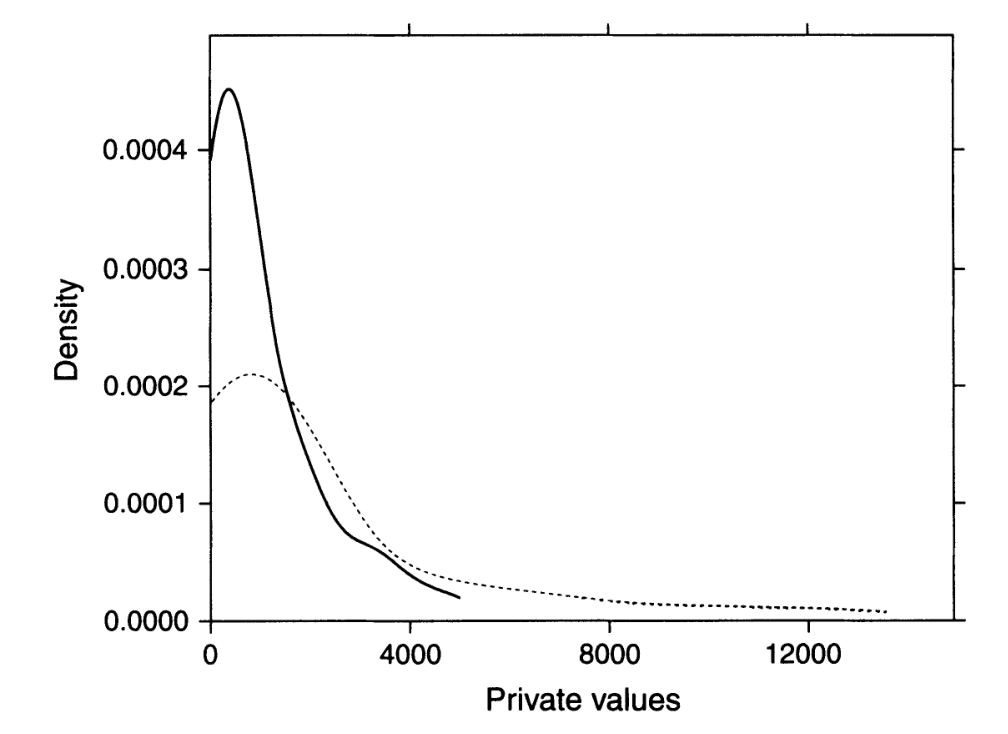
\includegraphics[width=\textwidth]{figures/ch15/cpv_fig2.png}
    \caption{Symmetric configurations: joint vs.\ joint (dashed), solo vs.\ solo (solid)}
  \end{subfigure}\hfill
  \begin{subfigure}[b]{0.48\textwidth}
    \centering
    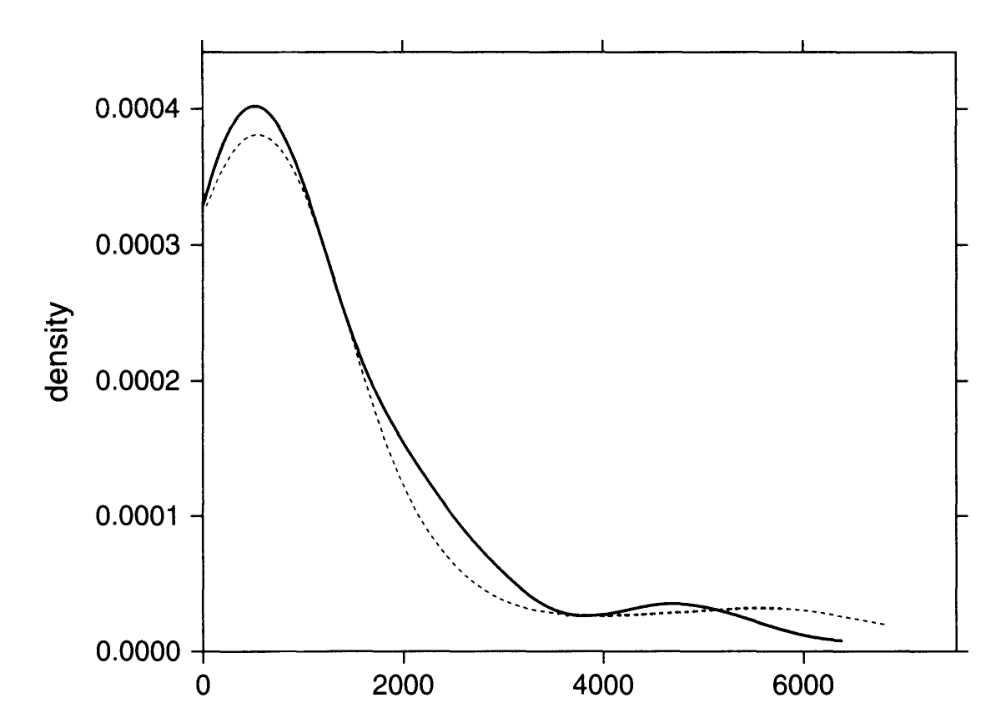
\includegraphics[width=\textwidth]{figures/ch15/cpv_fig4.png}
    \caption{Mixed configuration: joint (dashed), solo (solid)}
  \end{subfigure}
  \caption{Estimated marginal densities of private values in OCS wildcat auctions, dollars per acre. The
  horizontal axes differ across panels. In symmetric auctions the joint bidders' values are far more dispersed
  than the solo bidders'. In mixed auctions the two densities are close. The contrast between panels points to
  unobserved tract heterogeneity across configurations. Source: \citet{CampoPerrigneVuong2003}, Figures 2
  and 4.}\label{fig:15-cpv-xi}
\end{figure}

\casehead{Unobserved heterogeneity and rents} Under \cref{ass:15-cpv-uh}, comparing a type's value density
across configurations detects unobserved tract heterogeneity. Kolmogorov-Smirnov statistics are 0.1917 for
joint bidders in $(2,0)$ against $(1,1)$ auctions and 0.0965 for solo bidders in $(0,2)$ against $(1,1)$
auctions \citep[p.~200]{CampoPerrigneVuong2003}. The authors read the first as a clear rejection. Tracts
that attract two joint bidders are more valuable than tracts that attract one bidder of each type. The
differences in \cref{tab:15-cpv-stats} thus reflect both asymmetry and tract heterogeneity, with
heterogeneity the larger force. Winners' informational rents \eqref{eq:15-ir} average 65.07 percent across 197
winners (their Table II). They are 65.50 percent for joint and 64.59 percent for solo winners. So the
government captures about 35 percent of the winner's willingness to pay. In dollars, joint winners earn
\$1,954.42 per acre and solo winners \$1,151.40, because joint winners have higher values
\citep[p.~201]{CampoPerrigneVuong2003}.

\casehead{Interpretation and critiques} Asymmetry between joint and solo bidders is weak. A ban on joint bidding
would therefore change little if participation stayed the same. The authors argue that joint bidding raised
revenue by increasing participation. The paper's contribution is methodological. It shows that the indirect
approach handles asymmetric bidders whose equilibrium cannot be computed, and it gives a usable test of pure
common values. The limits are severe in practice. The trivariate objects in \eqref{eq:15-cpv-foc} force the
analysis to two-bidder auctions. With three bidders only 18 to 60 auctions would be available per
configuration (their footnote 16). Types are binary and the configuration is taken as exogenous to values
given the tract. The private value assumption for oil leases is contested. \citet{HendricksPinksePorter2003}
find bidding on earlier OCS auctions more consistent with common values (\cref{sec:15-cv-hp}).

\subsection{Asymmetric independent private values with all bids}\label{sec:15-apv-asym}

Independence simplifies the inversion and lowers data requirements. Let bidder $j$'s bid have distribution
$G_j$ and density $g_j$. With independent values, bids are independent, so
$G_{M_i\mid B_i}(m\mid b)=\prod_{j\ne i}G_j(m)$. Differentiating the product,
\begin{align*}
  g_{M_i\mid B_i}(m\mid b)&=\sum_{k\ne i}g_k(m)\prod_{j\ne i,k}G_j(m),\\
  \frac{G_{M_i\mid B_i}(b\mid b)}{g_{M_i\mid B_i}(b\mid b)}
  &=\frac{\prod_{j\ne i}G_j(b)}{\sum_{k\ne i}g_k(b)\prod_{j\ne i,k}G_j(b)}
  =\left[\sum_{j\ne i}\frac{g_j(b)}{G_j(b)}\right]^{-1}.
\end{align*}
The inverse bid function is therefore
\begin{equation}\label{eq:15-asym-xi}
  v_i=\xi_i(b_i)=b_i+\left[\sum_{j\ne i}\frac{g_j(b_i)}{G_j(b_i)}\right]^{-1},
\end{equation}
the inverse form of \eqref{eq:14-asym-foc}. Each value depends on its own bid and on the univariate
distributions of rivals' bids. When all bids and bidder identities are observed, each $F_i$ is identified
by $F_i(v)=G_i(\xi_i^{-1}(v))$ \citep[Theorem~3.1(ii)]{AtheyHaile2007}.

Estimation must condition on the set of opponents, because a change in their identities changes the
strategy being inverted. With fully bidder-specific distributions, each set of bidders is treated separately.
This requires many auctions with the same bidder set. A practical compromise groups bidders into a few
types, with exchangeability within a type, as with joint and solo bidders or loggers and mills
\citep[Section~3.2.2]{AtheyHaile2007}. All auctions with the same number of bidders of each type can then be
pooled. Asymmetry can also come from bidder covariates, such as the distance from a contractor's plant to the
project. With discrete covariates this is the approach by types again. With continuous covariates the bid
distributions are estimated conditional on them by kernel or sieve methods. The timber study of
\cref{sec:15-als} applies \eqref{eq:15-asym-xi} with parametric bid distributions.

\citet{FlambardPerrigne2006} apply the procurement version nonparametrically to snow removal contracts in
Montreal \citep[p.~102]{HortacsuPerrigne2021}. In a low-bid auction bidder $i$ wins when every rival bids
more, and the same steps give
\begin{equation*}
  c_i=b_i-\left[\sum_{j\ne i}\frac{g_j(b_i)}{1-G_j(b_i)}\right]^{-1}.
\end{equation*}
Firms are classified by their location relative to the job, and participation, winning probabilities and bid
distributions differ across the classes. The estimated cost difference between the classes is about 6.5
percent. It leads to an inefficient allocation in 24 percent of the auctions. A subsidy to the weak,
high-cost firms that restores symmetry would raise the share of contracts they win by 61 percent. With a cost
of public funds taken into account, the overall procurement cost would fall by 1.34 percent under exogenous
participation.

Equilibrium imposes testable restrictions. With independence and a common support of values,
\cref{thm:15-ah-rational} requires bids to be independent, each $\xi_i$ to be increasing, and all $\xi_i$ to
share the same upper endpoint. The last restriction comes from the common support. It can fail in a valid
equilibrium if supports differ. \citet[Section~5.1]{AtheyHaile2007} give an example, which we verify. Let
$n=2$ with bid distributions $G_1(b)=b$ and $G_2(b)=b^2$ on $[0,1]$. Then \eqref{eq:15-asym-xi} gives
\begin{equation*}
  \xi_1(b)=b+\frac{G_2(b)}{g_2(b)}=b+\frac b2=\frac32b,
  \qquad
  \xi_2(b)=b+\frac{G_1(b)}{g_1(b)}=2b .
\end{equation*}
The implied value distributions are $F_1(v)=G_1(\frac23v)=\frac23v$ on $[0,\frac32]$ and
$F_2(v)=G_2(\frac v2)=\frac{v^2}{4}$ on $[0,2]$. Each strategy is a best response. Bidder 1 maximizes
$(v-b)b^2$, so $v=\frac32b$, and bidder 2 maximizes $(v-b)b$, so $v=2b$. Yet $\xi_1(1)=\frac32\ne2=\xi_2(1)$.
Equivalently, the densities of the highest rival bid differ at the top, $g_{M_1}(1)=g_2(1)=2$ and
$g_{M_2}(1)=g_1(1)=1$, so the boundary condition \eqref{eq:15-boundary-test} fails.
Allowing supports to differ across bidders restores identification in such cases. If the lower ends of the
supports also differ, some bidders may never win, and little can be learned about them
\citep[Section~5.1]{AtheyHaile2007}.

\section{Common Values: Limits of Identification and Tests}\label{sec:15-cv}

With common values, information about each bidder's value is dispersed among the bidders. Learning a
rival's signal would change a bidder's estimate of her own value (\cref{def:14-private-values}). Winning then
carries bad news, the winner's curse of \cref{sec:14-winners-curse}. Many policy questions turn on the joint
distribution of signals and values. Examples are the optimal reserve price, the revenue ranking of formats,
and whether restricting entry raises revenue. This section first shows how little bids reveal about that
distribution. It then shows that exogenous variation in competition still allows private values to be tested
against common values. Next it presents a positive identification result for procurement with interdependent
costs \citep{Somaini2020}. It ends with the evidence of \citet{HendricksPorter1988} on an auction with an
informed bidder.

\subsection{What bids can and cannot reveal}\label{sec:15-cv-limits}

Let bidder $i$ observe a signal $S_i$ about her value $V_i$. The primitive is the joint distribution
$F_{\bm S,\bm V}$ of signals and values. In the pure common value model $V_i=V_0$ for all $i$. We focus on
symmetric models. Let $Y_i=\max_{j\ne i}S_j$ and define the \emph{pivotal expected value}
\begin{equation*}
  v(s,y;n)=\E\left[V_i\mid S_i=s,\ Y_i=y;\ n\right],
\end{equation*}
the expected value of a bidder whose signal is $s$ and whose strongest rival has signal $y$. The dimension
count is discouraging. The primitive governs $2n$ random variables, or $n+1$ with pure common values, yet an
auction reveals at most $n$ bids \citep[Section~7.1]{AtheyHaile2007}.

Signals have only ordinal meaning. Any strictly increasing relabeling of a signal leaves behavior unchanged.
\citet[eq.~(8)]{AtheyHaile2002} use this freedom to impose the normalization
\begin{equation}\label{eq:15-cv-norm}
  v(s,s;n)=\E\left[V_i\mid S_i=\max_{j\ne i}S_j=s;\ n\right]=s .
\end{equation}
In the second-price auction the equilibrium bid is $v(s,s;n)$ (\cref{prop:14-mw-spa}). Under
\eqref{eq:15-cv-norm} it becomes $b(s)=s$, so bids reveal signals. In the first-price auction, the
first-order condition of \eqref{eq:14-apv-foc} holds with the pivotal expected value on the left:
\begin{equation}\label{eq:15-cv-foc}
  v(s_i,s_i;n)=b_i+\frac{G_{M\mid B}(b_i\mid b_i)}{g_{M\mid B}(b_i\mid b_i)}
\end{equation}
\citep[eq.~(7.2)]{AtheyHaile2007}. The right side is the same functional of bids as in the APV model. All
bids therefore identify the joint distribution of the random variables $v(S_i,S_i;n)$, $i=1,\dots,n$, and
nothing more.

\begin{proposition}[{\citealp{LaffontVuong1996}}]\label{prop:15-lv}
Fix $n$ and suppose the reserve price does not bind. Every symmetric affiliated value model of the
first-price auction with a strictly increasing equilibrium is observationally equivalent to a symmetric APV
model. Its private values are $\tilde V_i=v(S_i,S_i;n)$.
\end{proposition}

\begin{proof}
Bids are strictly increasing transformations of affiliated, exchangeable signals, so $\bm G$ is symmetric and
affiliated. By \eqref{eq:15-cv-foc}, $\xi(b;\bm G)=v\bigl(\beta^{-1}(b),\beta^{-1}(b);n\bigr)$, which is
strictly increasing in $b$. At $b=\beta(s)$ the ratio in \eqref{eq:15-cv-foc} equals $v(s,s;n)-\beta(s)$, which vanishes at
$\underline s$ because $\beta(\underline s)=v(\underline s,\underline s;n)$ by \eqref{eq:14-mw-fpa-bid2}. Both
conditions and the boundary condition of \cref{prop:15-lpv} hold, so an APV structure rationalizes
$\bm G$. Its values are $\xi(B_i;\bm G)=v(S_i,S_i;n)$.
\end{proof}

Conclusions drawn from bids with a fixed set of bidders and no reserve price therefore rest on a maintained
assumption of private or common values. Different maintained assumptions can justify a wide range of reserve
prices as optimal \citep[Section~7.1]{AtheyHaile2007}. Second-price and ascending auctions do no better.

\begin{proposition}[{\citealp[Corollary~2]{AtheyHaile2002}}]\label{prop:15-cv-nonid}
Consider the symmetric common value model of the second-price sealed-bid auction.
\begin{enumerate}[label=(\roman*)]
  \item The distribution of signals $F_{\bm S}$ is not identified from bids unless all bids are observed.
  \item The joint distribution $F_{\bm S,\bm V}$ is not identified from bids.
\end{enumerate}
\end{proposition}

\begin{proof}
Under \eqref{eq:15-cv-norm} bids equal signals. Part (i) is then \cref{thm:15-ah4} applied to the exchangeable
vector $\bm S$. For (ii), take two joint distributions with the same $F_{\bm S}$ and different conditional
laws of $\bm V$ given $\bm S$, both satisfying \eqref{eq:15-cv-norm}. In both, $b(s)=s$, so the
distributions of bids coincide.
\end{proof}

Ascending auctions are harder still. A normalization like \eqref{eq:15-cv-norm} can hold only in the initial
phase, before anyone exits. After each exit, bidders revise their planned exit prices in ways that depend on
$F_{\bm S,\bm V}$. With $n>2$ there is also a continuum of symmetric equilibria in undominated strategies
\citep{BikhchandaniHaileRiley2002}. Even the most restrictive common value model fails.

\begin{proposition}[{\citealp[Theorem~8]{AtheyHaile2002}}]\label{prop:15-ah8}
In an ascending auction, assume pure common values, independent and identically distributed signals, and the
equilibrium of \citet{MilgromWeber1982}. With $n$ fixed, the model is not identified from the observed bids,
even up to a normalization of signals.
\end{proposition}

\begin{proof}
Take $n=3$ and signals uniform on $[0,1]$. Let $s^{(1:3)}\le s^{(2:3)}\le s^{(3:3)}$ be the ordered signals.
Model A has $V_0=\frac{s_1+s_2+s_3}{3}$. Model B has
$\hat V_0=\frac{s^{(1:3)}}{3}+\frac{s^{(2:3)}}{6}+\frac{s^{(3:3)}}{2}$. In the Milgrom-Weber equilibrium each
bidder initially plans to exit at the expected value given that all signals equal her own. In both models
\begin{equation*}
  \E[V_0\mid S_1=S_2=S_3=s]=s=\frac s3+\frac s6+\frac s2,
\end{equation*}
so the first exit occurs at $B^{(1:3)}=s^{(1:3)}$ in both. Its distribution is $1-(1-b)^3$. The first exit
reveals $s^{(1:3)}$. Each remaining bidder then plans to exit at the expected value given her own signal $y$, the
revealed signal $s$, and a remaining rival with signal $y$. In Model A this is $\frac{s+2y}{3}$. In Model B it
is $\frac s3+\frac y6+\frac y2=\frac{s+2y}{3}$. The second exit therefore has the same conditional distribution
given $B^{(1:3)}$ in both models. The winner never exits, so the joint distribution of observed bids is the
same in both models.
\end{proof}

The two models differ in economically relevant ways. The optimal reserve price differs between them
\citep[footnote~38]{AtheyHaile2002}. In Model B a bidder's value depends less on her rivals' signals when her
own signal is the highest. This lowers the participation threshold for any reserve price and changes the
seller's objective \citep[Section~7.1]{AtheyHaile2007}.

\casehead{Identification with more structure} One route adds structure. In the symmetric \emph{mineral rights
model}, signals are independent given the common value. \citet{LiPerrigneVuong2000} add separability. For each
$n$ there are known constants $C$ and $D>0$ such that, under \eqref{eq:15-cv-norm}, $S_i=C+D(V_0+A_i)$, with
$(V_0,A_1,\dots,A_n)$ mutually independent and the $A_i$ identically distributed
\citep[p.~2126]{AtheyHaile2002}. Then \eqref{eq:15-cv-foc} reads
\begin{equation*}
  C+D\,(v_0+a_i)=b_i+\frac{G_{M\mid B}(b_i\mid b_i)}{g_{M\mid B}(b_i\mid b_i)} .
\end{equation*}
All bids identify the joint distribution of $(V_0+A_1,\dots,V_0+A_n)$. When the characteristic functions do
not vanish, the deconvolution argument of \cref{lem:15-kotlarski} separates the distributions of $V_0$ and
$A_i$. The argument fails when some bids are missing. Bids then reveal order statistics $V_0+A^{(i:n)}$,
which are dependent even though the $A_i$ are independent.

\citet{LiPerrigneVuong2000} apply this structure to wildcat leases of the Outer Continental Shelf
\citep[p.~129]{HortacsuPerrigne2021}. They estimate two versions. In the conditionally independent
private values version, each bidder's value is its signal $S_i=V_0A_i$, with $V_0$ independent of the
$A_i$, so logs are additive as above. In the pure common value version, the pivotal expected value is
log-linear in the log signal, and the model is identified only up to location and scale. In the first
version the recovered values are multiple indicators of $V_0$, a measurement-error problem that
deconvolution solves. The estimates show little affiliation. The variance of $\ln V_0$ is only 9.2
percent of the variance of $\ln A_i$, so idiosyncratic factors explain most of the variation in values.

\casehead{Identification with ex post values} The other route adds data. In offshore oil auctions the oil
extracted is metered, and in scaled timber sales the harvested volume is recorded. Such data measure the
realized common value $v_0$ \citep[Section~7.2.2]{AtheyHaile2007}. Define the conditional mean of the ex post
value given the bid and the highest rival bid,
\begin{equation}\label{eq:15-hpp-vartheta}
  \vartheta(b,b';n)=\E\left[V_0\mid B_i=b,\ M_i=b';\ n\right].
\end{equation}
It is identified without any behavioral assumption, since $V_0$, $B_i$ and $M_i$ are all observed. With
monotone bidding, $\E[V_0\mid S_i=Y_i=s;n]=\vartheta(b,b;n)$ at $b=\beta(s;n)$. \Cref{eq:15-cv-foc}
then yields the overidentifying restriction
\begin{equation}\label{eq:15-hpp-test}
  \vartheta(b,b;n)=b+\frac{G_{M\mid B}(b\mid b)}{g_{M\mid B}(b\mid b)} .
\end{equation}
\citet{HendricksPinksePorter2003} proposed this test of equilibrium bidding. They estimate the left side by a
bivariate local linear regression of ex post values on $(B_i,M_i)$ and the right side from bids. Ex post values
also measure the winner's curse. Two natural measures are
\begin{equation*}
  \E[V_0\mid S_i=s]-\E[V_0\mid S_i=Y_i=s]
  \quad\text{and}\quad
  \E[V_0\mid S_i=s]-\E[V_0\mid S_i=s,\ Y_i\le s],
\end{equation*}
equations (7.5)--(7.6) of \citet{AtheyHaile2007}. In bid terms they are $\E[V_0\mid B_i=b]-\vartheta(b,b;n)$
and $\E[V_0\mid B_i=b]-\E[V_0\mid B_i=b,\,M_i\le b]$. The second uses only winning bids.

A positive value of the second measure does not reject private values
\citep[footnote~86]{AtheyHaile2007}. The interpretation of the measured ex post value as $V_0$ presumes common
values. Suppose values are independent and private and the measure equals the winner's value $\max_jV_j$. Then
$\E[\max_jV_j\mid V_i=v]-\E[\max_jV_j\mid V_i=v,\ \max_{k\ne i}V_k\le v]=\E[\max_jV_j\mid V_i=v]-v>0$. A noisy
measure $\tilde V_0=\lambda_0+\lambda_1V_0+\eta$ with $\E[\eta\mid\bm S]=0$ can still be used. The ex post
analogue of \eqref{eq:15-cv-norm} is then $\lambda_0+\lambda_1s$, which identifies $\lambda_0$ and $\lambda_1$
\citep[eq.~(7.11)]{AtheyHaile2007}.

\citet{HendricksPinksePorter2003} take both ideas to wildcat leases of the Outer Continental Shelf, where ex
post estimates of tract value measure $V_0$ \citep[p.~126]{HortacsuPerrigne2021}. Actual competition is low
relative to potential entry, so they build a data-driven measure of the number of potential bidders. They
estimate the expected ex post value given the bid, the level of competition and tract characteristics, and
then add the condition that every rival bid lies below the bid. The difference is the second measure above.
The winner's curse is about 107 percent of the average winning bid when competition is low, and it falls to
75 percent when competition is high. A second test compares conditional expectations of ex post values with
the pivotal expected values recovered from bids by the indirect approach, as in \eqref{eq:15-hpp-test}. The
recovered pivotal values rise with the bid, as rationalization requires, and bidders appear to overestimate
tract values when competition is low. The authors conclude that bidding is consistent with common values
and that bidders lower their bids to correct for the winner's curse.

\subsection{Testing private against common values}\label{sec:15-cv-tests}

Early tests regressed bids on the number of bidders \citep{GilleyKarels1981,Paarsch1992}. The idea was that
competition raises bids under private values, while a severe winner's curse could lower them under common
values. The idea fails twice. In first-price auctions, bids can rise or fall with $n$ under both paradigms
\citep{PinkseTan2005}. In ascending auctions the winner's value is censored. The distribution of each observed
order statistic shifts with $n$ even without a winner's curse, so the regression confounds the two effects
\citep[Section~8]{AtheyHaile2007}. The valid tests below isolate the winner's curse with an exact restriction
from probability theory.

\begin{lemma}[Recurrence relation, {\citealp[eq.~(9)]{AtheyHaile2002}}]\label{lem:15-recurrence}
Let $X_1,\dots,X_n$ be exchangeable with continuous marginal distributions, and let $F_{(r:k)}$ be the
distribution of the $r$-th lowest of $X_1,\dots,X_k$. Then for all $x$ and all $r\le n-1$,
\begin{equation}\label{eq:15-recurrence}
  \frac{n-r}{n}F_{(r:n)}(x)+\frac{r}{n}F_{(r+1:n)}(x)=F_{(r:n-1)}(x).
\end{equation}
\end{lemma}

\begin{proof}
Draw an index $J$ uniformly from $\{1,\dots,n\}$, independently of $\bm X$, and delete $X_J$. By
exchangeability, the remaining $n-1$ variables have the same joint law as $(X_1,\dots,X_{n-1})$. So the $r$-th
lowest of them, call it $\tilde X$, has distribution $F_{(r:n-1)}$. Let $R_J$ be the rank of $X_J$ among all
$n$ variables. Because $J$ is uniform and independent of $\bm X$, $R_J$ is uniform on $\{1,\dots,n\}$ and
independent of the order statistics $X^{(1:n)},\dots,X^{(n:n)}$. If $R_J>r$, deleting $X_J$ leaves the $r$
lowest variables intact, so $\tilde X=X^{(r:n)}$. This event has probability $\frac{n-r}{n}$. If $R_J\le r$,
one of the $r$ lowest is removed, so $\tilde X=X^{(r+1:n)}$. This event has probability $\frac rn$. Hence
\begin{equation*}
  F_{(r:n-1)}(x)=\Pr(\tilde X\le x)
  =\frac{n-r}{n}\Pr\bigl(X^{(r:n)}\le x\bigr)+\frac rn\Pr\bigl(X^{(r+1:n)}\le x\bigr).
\end{equation*}
\end{proof}

As a check, let $n=2$, $r=1$, and let the $X_i$ be independent with distribution $F$. Then
$\frac12[1-(1-F)^2]+\frac12F^2=\frac12(2F-F^2+F^2)=F=F_{(1:1)}$. Under private values the number of bidders
does not change values, so the distributions of value order statistics obey \eqref{eq:15-recurrence} across
$n$. Under common values the winner's curse breaks the relation in a known direction. The direction comes from
the following result. It assumes exogenous participation in the sense of \cref{sec:15-primitives}, so adding a
bidder leaves the joint distribution of the incumbents' signals and values unchanged.

\begin{lemma}[{\citealp[Lemma~8.1]{AtheyHaile2007}}]\label{lem:15-pivotal-n}
Suppose participation is exogenous. With private values, $v(s,s;n)=v(s,s;n+1)$ for all $s$. With symmetric
common values, $v(s,s;n)>v(s,s;n+1)$ for all $s$.
\end{lemma}

\begin{proof}
With private values $v(s,s;n)=\E[V_i\mid S_i=s]$, which does not depend on $n$. With common values, fix
bidder $i$, an incumbent rival $m$, and an entrant $j$. By symmetry,
\begin{align*}
  v(s,s;n)&=\E\left[V_i\mid S_i=s,\ S_m=s,\ S_k\le s\ \forall k\ne i,m\right]\\
  &=\E\Bigl[\E\left[V_i\mid S_i=s,\ S_m=s,\ S_k\le s\ \forall k\ne i,m,\ S_j\right]\Bigr]\\
  &>\E\left[V_i\mid S_i=s,\ S_m=s,\ S_k\le s\ \forall k\ne i,m,\ S_j\le s\right]
  =v(s,s;n+1).
\end{align*}
The second line is the law of iterated expectations over the entrant's signal. With common values the inner
expectation is strictly increasing in $S_j$. Restricting $S_j$ to $S_j\le s$ removes its highest
realizations and strictly lowers the mean. The last equality is the definition of $v$ with $n+1$ bidders,
since the event says that the strongest of $i$'s $n$ rivals has signal $s$.
\end{proof}

Winning against more rivals is worse news. With twenty bidders, having the highest signal implies a more
biased signal than with two. \Cref{fig:15-wc-n} illustrates \cref{lem:15-pivotal-n} in a Gaussian mineral
rights model.

\begin{theorem}[{\citealp[Theorem~9]{AtheyHaile2002}}]\label{thm:15-ah9}
In a second-price sealed-bid or ascending auction with exogenous participation, the symmetric private value
model is testable against the symmetric common value alternative. It suffices to observe the transaction price
$B^{(m-1:m)}$ in auctions with $m\ge2$ bidders and the bids $B^{(m-1:n)},\dots,B^{(n-1:n)}$ in auctions with
$n>m$ bidders.
\end{theorem}

\begin{proof}
Take a second-price auction and $m=n-1$. Each bidder bids $b(s;n)=v(s,s;n)$. Under private values $b(s;n)$
does not depend on $n$. Bids are then a fixed increasing transformation of exchangeable signals, so they are
exchangeable. Applying \eqref{eq:15-recurrence} with $r=n-2$ gives
\begin{equation}\label{eq:15-ah-10}
  \frac2n\Pr\bigl(B^{(n-2:n)}\le b\bigr)+\frac{n-2}{n}\Pr\bigl(B^{(n-1:n)}\le b\bigr)=\Pr\bigl(B^{(n-2:n-1)}\le b\bigr).
\end{equation}
Under common values, $b(s;n)<b(s;n-1)$ by \cref{lem:15-pivotal-n}. Let $\sigma_k(b)$ be the signal that bids
$b$ in a $k$-bidder auction, so $\sigma_n(b)>\sigma_{n-1}(b)$. Using \eqref{eq:15-recurrence} for signals,
\begin{align*}
  \frac2n\Pr\bigl(B^{(n-2:n)}\le b\bigr)+\frac{n-2}{n}\Pr\bigl(B^{(n-1:n)}\le b\bigr)
  &=\frac2nF_{(n-2:n)}\bigl(\sigma_n(b)\bigr)+\frac{n-2}{n}F_{(n-1:n)}\bigl(\sigma_n(b)\bigr)\\
  &=F_{(n-2:n-1)}\bigl(\sigma_n(b)\bigr)\\
  &>F_{(n-2:n-1)}\bigl(\sigma_{n-1}(b)\bigr)=\Pr\bigl(B^{(n-2:n-1)}\le b\bigr),
\end{align*}
where $F_{(r:k)}$ now refers to signals. A test of the equality \eqref{eq:15-ah-10} against this first-order
stochastic dominance tests private against common values. In the ascending auction, private values again
imply \eqref{eq:15-ah-10} and hence the recurrence in means,
$\E[B^{(n-2:n-1)}]=\frac2n\E[B^{(n-2:n)}]+\frac{n-2}{n}\E[B^{(n-1:n)}]$. Under common values the top losing
bidder in an $(n-1)$-bidder auction exits later in expectation than she would with an extra rival. This yields
the strict inequality $\E[B^{(n-2:n-1)}]>\frac2n\E[B^{(n-2:n)}]+\frac{n-2}{n}\E[B^{(n-1:n)}]$ in every symmetric
separating equilibrium \citep[eqs.~(13)--(17)]{AtheyHaile2002}.
\end{proof}

The ascending-auction part is notable because it holds whatever equilibrium is played. The relevant
transaction price is the same in all symmetric separating equilibria, and Milgrom-Weber bids are maximal among
them \citep{BikhchandaniHaileRiley2002}. One caveat applies. Losing bids in real ascending auctions may
understate willingness to pay (\cref{thm:15-ht}), and this alone could mimic a winner's curse. Three
extensions follow.

\begin{theorem}[{\citealp[Theorems~10--11 and Corollary~4]{AtheyHaile2002}}]\label{thm:15-ah11}
Suppose participation is exogenous.
\begin{enumerate}[label=(\roman*)]
  \item \emph{Asymmetric bidders.} Consider a second-price auction. Suppose bids $B^{(m-1:n)},\dots,B^{(n-1:n)}$
  are observed in auctions with $n\ge3$ bidders, and transaction prices in auctions whose bidders form subsets of
  size $m<n$. Then the unrestricted private value model is testable against common values.
  \item \emph{First-price auctions.} If the top two bids are observed in auctions with $n$ and $n-1$ bidders,
  $n\ge3$, the symmetric APV model is testable against symmetric common values.
  \item \emph{Reserve prices.} Consider first-price, second-price or ascending auctions with a reserve price.
  Suppose $B^{(j:n)}$ and $B^{(j+1:n)}$ are observed in $n$-bidder auctions and $B^{(j:n-1)}$ in $(n-1)$-bidder
  auctions, for some $2\le j<n$. Then the symmetric private value model is testable.
\end{enumerate}
\end{theorem}

\begin{proof}[Proof sketch]
(i) A random subsample of size $m$ drawn from any $n$ random variables is exchangeable
\citep[proof of Theorem~10]{AtheyHaile2002}. The recurrence therefore holds for averages of order-statistic
distributions over subsets of bidders. (ii) Let $F_{v,(k:m)}$ be the distribution of
$v(S^{(k:m)},S^{(k:m)};m)$ in $m$-bidder auctions. By \cref{prop:15-top2} and \eqref{eq:15-cv-foc}, the top two
bids identify $F_{v,(n-1:n)}$, $F_{v,(n:n)}$ and $F_{v,(n-1:n-1)}$. Under private values these are distributions
of value order statistics, so by \eqref{eq:15-recurrence} with $r=n-1$,
\begin{equation*}
  \frac1nF_{v,(n-1:n)}(t)+\frac{n-1}{n}F_{v,(n:n)}(t)=F_{v,(n-1:n-1)}(t)\quad\text{for all } t .
\end{equation*}
Under common values $v(s,s;n)$ is still increasing in $s$, so the variables $v(S_i,S_i;n)$ are exchangeable and
obey the recurrence with $n$ held fixed. By \cref{lem:15-pivotal-n}, $v(s,s;n)<v(s,s;n-1)$, so the left side
strictly exceeds the right side. (iii) With a reserve price, participants' values are draws from the
distribution truncated at the reserve. Truncation preserves exchangeability, so the recurrence still holds
under private values \citep[proof of Corollary~4]{AtheyHaile2002}. In a first-price auction the relation applies
to the values recovered from the bids.
\end{proof}

When all bids of a first-price auction are observed, the test can use the whole distribution of pivotal
expected values. Let $F_{v,n}$ denote the distribution of the random variable $v(S_i,S_i;n)$, which
\eqref{eq:15-cv-foc} identifies.

\begin{proposition}[{\citealp[Corollary~8.1]{AtheyHaile2007} and \citealp{HaileHongShum2003}}]\label{prop:15-hhs}
Suppose participation is exogenous. Under private values, $F_{v,n}$ does not depend on $n$. Under symmetric
common values, $F_{v,n}(t)<F_{v,n+1}(t)$ for all $t$ in the interior of the supports.
\end{proposition}

The result follows from \cref{lem:15-pivotal-n}, since $v(S_i,S_i;n)$ falls with $n$ for every signal.
\citet{HaileHongShum2003} build a two-step test on it. The first step computes pseudo-values $\hat v_{it}$
separately for each $n$, as in \eqref{eq:15-lpv-pseudo}. The second step compares their empirical
distributions across $n$. Two statistics are proposed. The first compares quantile-trimmed means
\begin{equation*}
  \hat\mu_{n,\tau}=\frac{1}{nT_n}\sum_{t:\,n_t=n}\ \sum_{i=1}^{n}\indic\bigl(b_{it}\in[b_\tau,b_{1-\tau}]\bigr)\,\hat v_{it},
\end{equation*}
where $b_\tau$ is the $\tau$-th quantile of bids in $n$-bidder auctions. The null hypothesis is that the
$\mu_{n,\tau}$ are equal across $n$, and the alternative is that they decrease. Trimming at the same quantiles
for every $n$ fixes the set of signals behind each mean. Trimming on a fixed range of bids would compare
different signals and could create or hide a winner's curse. The vector of trimmed means is asymptotically
normal with a diagonal covariance matrix, which permits a one-sided likelihood ratio test. The second statistic
is a smoothed multi-sample one-sided Kolmogorov-Smirnov statistic,
$\sum_n\sup_v[\hat F_{\hat v,n+1}(v)-\hat F_{\hat v,n}(v)]$, with cutoffs obtained by subsampling
\citep[Section~8.1]{AtheyHaile2007}. Both tests must account for the estimation error in the pseudo-values.

\begin{figure}[htbp]
  \centering
  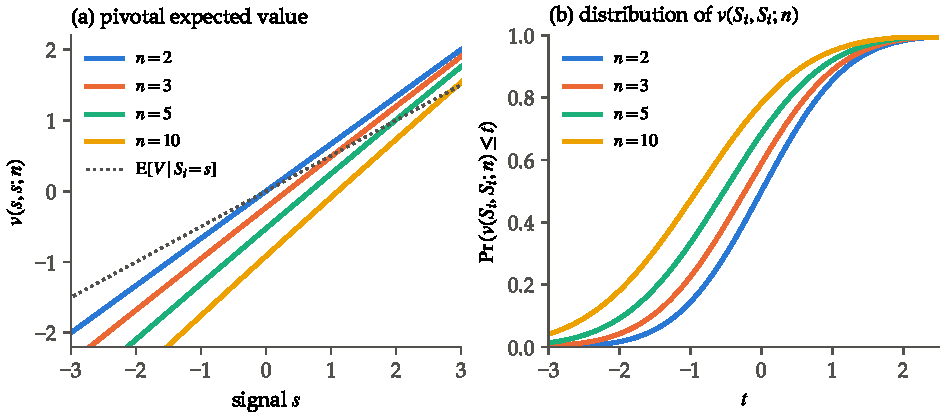
\includegraphics[width=\textwidth]{figures/ch15/cv_winners_curse.pdf}
  \caption{The winner's curse and the number of bidders in a Gaussian mineral rights model: $V_0\sim N(0,1)$
  and $S_i=V_0+e_i$ with independent $e_i\sim N(0,1)$. Panel (a): the pivotal expected value $v(s,s;n)$ falls
  with $n$ for every signal (\cref{lem:15-pivotal-n}). The dotted line is $\E[V_0\mid S_i=s]=\frac s2$, which
  does not depend on $n$. Panel (b): the distribution of $v(S_i,S_i;n)$, the object compared across $n$ in the
  test of \citet{HaileHongShum2003}. Under private values the four curves would coincide. Our computation by
  numerical integration, with no random numbers (script \texttt{cv\_winners\_curse.py}).}\label{fig:15-wc-n}
\end{figure}

\casehead{Endogenous participation} Exogenous variation in $n$ is a strong assumption. A binding reserve price
or a bid-preparation cost truncates the set of participating types. \citet{HaileHongShum2003} adjust for
truncation and compare the distributions on their common support \citep[Section~8.2]{AtheyHaile2007}.
Unobservables that move both participation and values are harder. If more valuable tracts attract more bidders,
that variation can mask the winner's curse. Unobserved heterogeneity also threatens identification of $F_{v,n}$
itself (\cref{sec:15-uh}). \citet{HaileHongShum2003} propose an instrumental approach that builds on
\cref{ass:15-cpv-uh}. Let the number of bidders be $n_t=\chi(Z_t,\omega_t)$, where $Z_t$ is observed and
$\omega_t$ is an unobserved index of the auction, the unobserved heterogeneity of \cref{sec:15-uh}. Assume
(i) $Z_t$ is independent of signals and values, and (ii) $\chi$ is weakly increasing in $Z_t$ and strictly
increasing in $\omega_t$. Strict monotonicity in $\omega_t$ makes $(n_t,Z_t)$ a sufficient statistic for
$\omega_t$. The pivotal expected value of a bidder whose signal $s$ leads to the bid $b$ is then identified
conditional on $(n_t,Z_t)$:
\begin{equation*}
  v(s,s;n,z)=b+\frac{\Pr\bigl(M_{it}\le b\mid B_{it}=b,\ Z_t=z,\ n_t=n\bigr)}{\frac{\partial}{\partial m}
  \Pr\bigl(M_{it}\le m\mid B_{it}=b,\ Z_t=z,\ n_t=n\bigr)\big|_{m=b}} .
\end{equation*}
Pooling pseudo-values across $n$ for each $z$, the distribution of pivotal values must be the same for all $z$
under private values. It shifts with $z$ under common values. In timber auctions they use the number of
sawmills and logging firms near a sale as the instrument \citep[Section~8.2]{AtheyHaile2007}. Strict
monotonicity in a scalar unobservable is the price of the approach. It also requires the unobservable to be
discrete, because $n_t$ is.

\casehead{Binding reserve prices} A reserve price offers a different test \citep{HendricksPinksePorter2003}.
With reserve $r$ in a symmetric first-price auction, a bidder participates if her signal exceeds the threshold
$s^\ast=\inf\{s:\E[V_i\mid S_i=s,\ Y_i\le s]\ge r\}$. The marginal participant bids $r$ and wins only when no rival
participates. Her pivotal expected value is $v(s^\ast,s^\ast;n)$. Under private values the two conditional
expectations coincide, so $v(s^\ast,s^\ast;n)=r$. Under common values
$\E[V_i\mid S_i=s^\ast,\ Y_i\le s^\ast]<\E[V_i\mid S_i=Y_i=s^\ast]$, so $v(s^\ast,s^\ast;n)>r$
\citep[eqs.~(8.7)--(8.8)]{AtheyHaile2007}. The inverse bid function at the bottom of the bid support,
$\lim_{b\downarrow r}\bigl[b+\frac{G_{M\mid B}(b\mid b)}{g_{M\mid B}(b\mid b)}\bigr]$, should equal $r$ under
private values and exceed it under common values. With private values the markdown vanishes at the reserve,
so rival bids are dense just above $r$ (compare \cref{thm:15-gpv-reserve}). With common values the markdown
stays positive, because even the marginal participant bids below her pivotal value. Bids just above $r$ are
then relatively sparse, an implication of the reserve price already noted by \citet{MilgromWeber1982}.
\citet{HillShneyerov2013} develop a formal test based on the tail of the bid distribution near the reserve.

\casehead{Evidence from timber, oil and procurement auctions} The tests have been applied in several
markets, and the answer depends on the market \citep[Sections~2.3, 3.2 and 4.1]{HortacsuPerrigne2021}. In
Forest Service first-price sales in the western half of the United States, the tests of
\citet{HaileHongShum2003} find no evidence of common values in scale sales. We report the results of the
2006 revision of that working paper, as summarized by \citet[pp.~93--94]{HortacsuPerrigne2021}. The evidence is
mixed in lump-sum sales, where the case for common values was stronger.
\citet{CompianiHaileSantAnna2020} extend the test to endogenous entry and unobserved heterogeneity and apply
it to Outer Continental Shelf leases (pp.~126--127). Private information is multiplicatively separable into a
function of observed and unobserved heterogeneity and an idiosyncratic base value. Bids then decompose into
the same function times a \emph{homogenized bid} that depends only on the number of bidders and the signal.
The number of bidders depends on observables and rises weakly with the unobservable. An instrument shifts
entry but not signals or values, and in the application it is the number of neighbor firms. Under private
values the joint distribution of signals and values does not depend on the number of bidders, while common
values order it by stochastic dominance. The authors conclude in favor of common values. Ignoring unobserved
heterogeneity would produce an ordering contrary to common values, a misspecification of the kind studied in
\cref{sec:15-uh}. For policy, the seller would not gain from limiting competition to soften the winner's
curse. A second-price auction, which exploits the linkage principle (\cref{prop:14-linkage}), would raise
revenue only slightly.

\citet{HongShum2002} quantify the winner's curse in procurement with a parametric model of affiliated values
(pp.~104--105). Under common values more bidders have two effects on bids. A competitive effect lowers them,
and a winner's-curse effect raises them, so bids can be U-shaped in the number of bidders. The model follows
the log-additive specification of Wilson, with multiplicative decompositions of costs and signals. The
relative standard deviations of the common component, the private component and the signal noise measure
how common the costs are. In New Jersey Department of Transportation auctions, highway work behaves like
common values, while bridge work and road paving mix private and common values. Allowing for unobserved
heterogeneity, road paving looks like independent private costs and highway work like affiliated private
values. For highway work, halving the number of bidders would lower the procurement cost by 15 percent. For
the other two kinds of work, more competition lowers the cost, so the competitive effect dominates.

\Cref{tab:15-cv-tests} collects the tests of this subsection. Each one replaces the unattainable goal of
identifying $F_{\bm S,\bm V}$ by a restriction that private values impose and common values violate.

\begin{table}[htbp]
\centering
\caption{Tests of private against common values}\label{tab:15-cv-tests}
\small
\begin{tabularx}{\textwidth}{@{}>{\raggedright\arraybackslash}p{2.6cm}>{\raggedright\arraybackslash}X>{\raggedright\arraybackslash}X>{\raggedright\arraybackslash}p{2.5cm}@{}}
\toprule
Format & Data and variation & Restriction under private values & Source \\
\midrule
Second-price or ascending & Price with $m$ bidders, upper bids with $n>m$. Exogenous $n$ & Recurrence
\eqref{eq:15-recurrence} holds (in means for ascending). Common values give dominance & \citet[Thm.~9]{AtheyHaile2002} \\
Second-price, asymmetric & Bids with $n$ bidders, prices with subsets of bidders & Recurrence for random
subsamples & \citet[Thm.~10]{AtheyHaile2002} \\
First-price & Top two bids with $n$ and $n-1$ bidders & Recurrence for identified $v(S,S;n)$ & \citet[Thm.~11]{AtheyHaile2002} \\
First-price & All bids, exogenous $n$ & $F_{v,n}$ invariant to $n$. It falls in $n$ under common values &
\citet{HaileHongShum2003} \\
First-price & All bids, instrument for $n$ & Pivotal values invariant to the instrument & \citet{HaileHongShum2003} \\
First-price & All bids, instrument for entry, unobserved heterogeneity & Joint law of signals and values invariant to $n$ & \citet{CompianiHaileSantAnna2020} \\
First-price & Binding reserve price & Inverse bid function equals $r$ at the bottom & \citet{HendricksPinksePorter2003} \\
First-price & All bids and ex post values & Overidentifying restriction \eqref{eq:15-hpp-test} & \citet{HendricksPinksePorter2003} \\
First-price, two bidders & Bids and identities & Quasi-symmetry rejects asymmetric pure common values & \citet{CampoPerrigneVuong2003} \\
\bottomrule
\end{tabularx}
\end{table}

\subsection{Interdependent costs: Somaini (2020)}\label{sec:15-cv-somaini}

\casehead{Question} Most empirical work picks one of two polar models. Under private costs there is no
winner's curse. Under pure common costs every bidder would incur the same cost, so the allocation cannot be
inefficient. Intermediate models had received little attention, largely because \citet{LaffontVuong1996}
showed that any bid distribution rationalized by interdependent costs is also rationalized by private costs.
\citet{Somaini2020} asks whether richer variation in competitive conditions restores identification in
procurement auctions. The variation comes from continuous bidder-specific cost shifters, such as each firm's
distance to the project. The test of \citet{HaileHongShum2003} uses discrete variation in $n$. Continuous
shifters vary competition in more directions.

\casehead{Primitives} A buyer procures a project by first-price (low-bid) sealed bid from $n$ risk-neutral
bidders, with no reserve price. Bidder $i$'s cost is $C_i$ and her private information is a scalar signal
$S_i$. Signals are normalized to have uniform marginals, so their joint distribution $F_{\bm S}$ is a copula.
Each bidder has a public cost shifter $w_i$, and $\bm w=(w_1,\dots,w_n)$. Somaini writes $x_i$ for $w_i$ and
conditions on auction characteristics throughout. Bidder $i$'s \emph{full-information cost} is
\begin{equation*}
  c_i(\bm s_{-i},s_i,w_i)=\E\left[C_i\mid \bm S=\bm s,\ \bm w\right].
\end{equation*}
For risk-neutral bidders, the payoff-relevant primitives are $F_{\bm S}$ and the functions $c_i$. They are
coarser than the joint distribution of costs and signals. They suffice for counterfactuals that change the rules,
the reserve price or subsidies \citep[Section~I]{Somaini2020}.

\begin{assumption}[{\citealp[Assumptions~A1--A3 and A7]{Somaini2020}}]\label{ass:15-somaini}
(A1) Signals are independent of cost shifters: $F_{\bm S\mid\bm w}=F_{\bm S}$. (A2) Signals are scalar, and
$F_{\bm S}$ has a continuously differentiable bounded density $f$. (A3) Rivals' shifters are excluded from a
bidder's full-information cost: $\E[C_i\mid\bm S,\bm w]=c_i(\bm S_{-i},S_i,w_i)$. (A7) For every $\bm w$, the
data are generated by repeated play of the same Bayes-Nash equilibrium in monotone pure strategies.
\end{assumption}

The model nests the standard cases. Private costs mean $c_i$ does not depend on $\bm s_{-i}$. Independent
private costs add independence of signals, and affiliated private costs allow affiliation. Pure common costs
mean $c_i=c_j$ for all $i,j$. Bidders may also be asymmetric in any way. Assumptions A1 and A3 define what makes
an observable a cost shifter. For distance, they rule out a firm having lower costs when a rival is nearby. They
also rule out a firm regarding a nearby rival's signal as more informative. Equilibria in monotone pure strategies
exist when signals are affiliated \citep{RenyZamir2004}. Somaini shows that without a binding reserve price they
are strictly increasing \citep[Proposition~1]{Somaini2020}.

\casehead{First-order condition} Let $s_j(b)=\beta_j^{-1}(b)$ be the signal at which rival $j$ bids $b$. A low
bid wins, so bidder $i$ wins with bid $b$ when $\bm S_{-i}\ge\bm s_{-i}(b)$ componentwise. Her expected
profit is
\begin{equation*}
  \Pi_i(b;s_i)=\int_{\bm\tau\ge\bm s_{-i}(b)}\bigl(b-c_i(\bm\tau,s_i,w_i)\bigr)f(\bm\tau\mid s_i)\,d\bm\tau .
\end{equation*}
Differentiating in $b$ gives one term from the margin $b$ and one boundary term for each rival:
\begin{multline*}
  \Pr\bigl(\bm S_{-i}\ge\bm s_{-i}(b)\mid s_i\bigr)
  -\sum_{j\ne i}s_j'(b)f\bigl(s_j(b)\mid s_i\bigr)\Pr\bigl(\bm S_{-ij}\ge\bm s_{-ij}(b)\mid s_i,s_j(b)\bigr)\\
  \times\Bigl[b-\E\bigl(C_i\mid s_i,\,s_j(b),\,\bm S_{-ij}\ge\bm s_{-ij}(b)\bigr)\Bigr]=0 .
\end{multline*}
Let $D_i(b)$ be the sum of the weights $s_j'(b)f(s_j(b)\mid s_i)\Pr(\bm S_{-ij}\ge\bm s_{-ij}(b)\mid s_i,s_j(b))$.
It equals the absolute derivative of the win probability in the bid. Let $\pi^{(i)}_j(b)$ be rival $j$'s weight
divided by $D_i(b)$. Rearranging,
\begin{equation}\label{eq:15-som-foc}
  b-\frac{\Pr\bigl(\bm S_{-i}\ge\bm s_{-i}(b)\mid s_i\bigr)}{D_i(b)}
  =\sum_{j\ne i}\pi^{(i)}_j(b)\,\E\Bigl(C_i\mid s_i,\ S_j=s_j(b),\ \bm S_{-ij}\ge\bm s_{-ij}(b),\ w_i\Bigr),
\end{equation}
equation (5) of \citet{Somaini2020}. The left side is marginal revenue, the bid minus a markup. The right side
is the expected cost conditional on the bid being \emph{pivotal}, that is, tying with at least one rival for the
lowest bid. The weight $\pi^{(i)}_j$ is the probability of tying with rival $j$ given a tie with at least one
rival.

\casehead{Identification} The argument has three steps. First, monotone strategies imply that the copula of bids
equals the copula of signals. With uniform signals, $s_i=H_{B_i\mid\bm w}(b_i)$, the marginal distribution of
$i$'s bid given $\bm w$. Hence $F_{\bm S}(\bm s)=H_{\bm B\mid\bm w}\bigl(Q_{B_1\mid\bm w}(s_1),\dots,Q_{B_n\mid\bm
w}(s_n)\bigr)$, where $Q$ denotes a quantile function \citep[Lemma~1 and Proposition~3]{Somaini2020}. By A1, the
bid copula must not vary with $\bm w$, a testable implication. Nonparticipation is recorded as an infinite bid.

Second, the left side of \eqref{eq:15-som-foc} is identified as in \eqref{eq:15-lpv-foc}, because conditioning on
the signal is conditioning on the bid. With $M_i=\min_{j\ne i}B_j$,
\begin{equation}\label{eq:15-som-xi}
  \xi_i(b_i,\bm w)=b_i-\frac{\Pr(M_i\ge b_i\mid B_i=b_i,\bm w)}{\bigl|\frac{\partial}{\partial m}\Pr(M_i\ge m\mid
  B_i=b_i,\bm w)\big|_{m=b_i}\bigr|} .
\end{equation}
The right side is the limit as $\varepsilon\downarrow0$ of $\E\bigl(C_i\mid S_i=s_i,\ \bm S_{-i}\in
L_\varepsilon(b_i,\bm w),\ w_i\bigr)$. Here $L_\varepsilon(b,\bm w)$ is the set of rival signals for which $i$ wins
with bid $b$ but loses with $b+\varepsilon$. It is the difference of two rectangles, each identified from the
marginal bid distributions.

Third, variation in rivals' shifters moves these sets. With two bidders the pivotal event is a single point, and
\eqref{eq:15-som-foc} becomes
\begin{equation}\label{eq:15-som-two}
  \xi_1(b_1,\bm w)=c_1\bigl(H_{B_2\mid\bm w}(b_1),\,H_{B_1\mid\bm w}(b_1),\,w_1\bigr),
\end{equation}
equation (8) of \citet{Somaini2020}. Holding $w_1$ fixed and varying $(w_2,b_1)$ evaluates $c_1(\cdot,\cdot,w_1)$
at different pairs of signals. A3 ensures that $w_2$ moves the evaluation point without shifting $c_1$ itself. The
rival's shifter works like an instrument for the rival's signal.

With three bidders the pivotal set is L-shaped (\cref{fig:15-som-L}). One bid gives one equation in two
unknowns, the expected costs conditional on tying with bidder 2 or with bidder 3. Different rival shifters
$\bm w'$ produce another L-shaped set stacked on the first, with $s_1$ and $w_1$ fixed. Under A1, the expected
cost over the union is a probability-weighted average with identified weights. Stacking ever finer L-shaped sets
covers the rectangle $\{S_2\ge s_2,\ S_3\ge s_3\}$. The limit identifies $\E(C_1\mid s_1,\ S_2\ge s_2,\ S_3\ge
s_3,\ w_1)$, the expected cost conditional on winning. Differentiating twice recovers the full-information cost:
\begin{multline}\label{eq:15-som-diff}
  \frac{\partial^2}{\partial s_2\,\partial s_3}\Bigl[\E\bigl(C_1\mid s_1,S_2\ge s_2,S_3\ge s_3,w_1\bigr)
  \Pr\bigl(S_2\ge s_2,S_3\ge s_3\mid s_1\bigr)\Bigr]\\
  =c_1(s_2,s_3,s_1,w_1)\,f_{S_2,S_3\mid S_1}(s_2,s_3),
\end{multline}
equation (10) of \citet{Somaini2020}. The two minus signs from differentiating the lower limits cancel.

\begin{figure}[htbp]
\centering
\begin{tikzpicture}[scale=5.2,>=Stealth]
  \fill[blue!8] (0.42,0.30) rectangle (1,1);
  \fill[blue!35] (0.42,0.30) -- (1,0.30) -- (1,0.36) -- (0.48,0.36) -- (0.48,1) -- (0.42,1) -- cycle;
  \fill[orange!45] (0.48,0.36) -- (1,0.36) -- (1,0.42) -- (0.54,0.42) -- (0.54,1) -- (0.48,1) -- cycle;
  \draw[thick] (0,0) rectangle (1,1);
  \draw (0.42,0.30) rectangle (1,1);
  \draw (0.48,0.36) rectangle (1,1);
  \draw (0.54,0.42) rectangle (1,1);
  \fill (0.42,0.30) circle (0.010);
  \fill (0.48,0.36) circle (0.010);
  \node[below left] at (0,0) {$0$};
  \node[below] at (1,0) {$1$};
  \node[left] at (0,1) {$1$};
  \node[below] at (0.5,-0.06) {rival signal $S_2$};
  \node[rotate=90] at (-0.1,0.5) {rival signal $S_3$};
  \node[font=\small] at (0.20,0.12) {$\bigl(s_2(b),s_3(b)\bigr)$};
  \draw[->] (0.24,0.16) -- (0.41,0.29);
  \node[font=\small] at (0.78,0.12) {$L_\varepsilon(b,\bm w)$};
  \draw[->] (0.78,0.16) -- (0.78,0.32);
  \node[font=\small,anchor=east] at (0.31,0.66) {$L_\varepsilon(t,\bm w')$};
  \draw[->] (0.32,0.66) -- (0.505,0.66);
  \node[font=\small,align=center] at (0.77,0.72) {win region\\ not yet\\ covered};
\end{tikzpicture}
\caption{Pivotal sets with three bidders in a procurement auction, drawn in the space of bidder 1's rivals'
signals. Bidder 1 wins with bid $b$ when both rival signals exceed the thresholds $s_2(b)$ and $s_3(b)$. The
blue L-shaped set $L_\varepsilon(b,\bm w)$ contains the rival signals for which bidder 1 wins with $b$ but loses
with $b+\varepsilon$. The first-order condition identifies the expected cost on this set. Different rival
shifters $\bm w'$ and a bid $t$ produce the stacked orange set $L_\varepsilon(t,\bm w')$, holding bidder 1's
signal and shifter fixed. Stacking such sets fills the light rectangle. Our drawing, after \citet[Figures~1--2]{Somaini2020}.}\label{fig:15-som-L}
\end{figure}

\begin{theorem}[{\citealp[Theorem~4]{Somaini2020}}]\label{thm:15-somaini}
Under \cref{ass:15-somaini}, the full-information cost $c_i(\bm s_{-i},s_i,w_i)$ is identified for all
$\bm s\ge\bm s^\ast$ if the observables exhibit sufficient variation and nonvanishing competition for bidder $i$
at $(\bm s^\ast,w_i)$.
\end{theorem}

Sufficient variation has a precise meaning \citep[Definition~1]{Somaini2020}. For every $\bm s\ge\bm s^\ast$
there must be rival shifters $\bm w_{-i}$ and a finite bid $b$ with $H_{B_j\mid\bm w}(b)=s_j$ for every bidder
$j$. The bid $b$ is then bidder $i$'s equilibrium bid at signal $s_i$. Nonvanishing competition bounds the number of L-shaped sets
needed, by requiring rivals to bid in any interval $[b,b']$ with nonvanishing probability (Definition~2).
Equilibrium observables of first-price auctions typically exhibit nonvanishing competition. A bounded set of
shifters suffices for signals bounded away from zero \citep[Propositions~5--6]{Somaini2020}. Identification at
extreme signals may need shifters with unbounded support.

Three limits deserve mention \citep[Section~III.C]{Somaini2020}. Binding reserve prices can reduce the variation
that shifters generate. Entry costs paid after learning signals are hard to distinguish from full-information
costs that rise sharply as rivals' signals approach the top. A random entry cost unobserved by the econometrician
violates A7, so \cref{thm:15-somaini} does not apply. Finally, the identified primitives cannot evaluate
counterfactuals in which bidders act after learning more, such as resale or subcontracting once costs are known.

\casehead{Setting and data} The Michigan Department of Transportation (MDOT) awards about 1,050 highway contracts
a year, worth about \$1.2 billion in total, by first-price sealed bid. On each monthly letting date, 150 to 200
firms bid on 50 to 70 contracts \citep[p.~3844]{Somaini2020}. Contracts are advertised at least 45 days ahead.
There is no formal reserve price, but the agency may reject all bids if the lowest exceeds 110 percent of the
engineer's estimate. From 2001 to 2010 the lowest bid exceeded that level in 11 percent of cases, and 15 percent
of these were rejected (p.~3845). The study focuses on hot-mixed asphalt paving. The mix must be compacted while
hot, above $135^\circ$C, so trucking time from a firm's plant matters for cost and quality. Distance from the plant
to the project is the cost shifter. Of 10,522 auctions from January 2001 to December 2010, 3,851 required asphalt
prequalification, and 1,925 had it as the only requirement. These form the sample (p.~3846).

In the sample the median engineer's estimate is \$633,000 and the median lowest bid \$586,000. Auctions have 3.04
participants on average. The median normalized winning bid, $\frac{\text{lowest bid}}{\text{estimate}}-1$, is
$-6.8$ percent. The second-lowest bid exceeds the lowest by 8.2 percent on average. The median participant is 38
km from the project and the median winner 22 km (Table~1). The average winning bid falls with the number of
participants, but the average bid does not (Table~2). Somaini reads this as evidence against the symmetric
independent private cost model with exogenous participation.

\casehead{Econometric model} Signals are mapped to standard normals, $\zeta_i=\Phi^{-1}(S_i)$, with
$\bm\zeta\sim N(0,\Sigma)$ and a factor structure $\Sigma=LL^\top+\Lambda$. Let $Z_t$ be auction characteristics.
The Gaussian information structure implies
\begin{equation}\label{eq:15-som-gauss}
  \E\bigl(C_i\mid\bm\zeta,Z_t,w_i\bigr)=\alpha_{ic}+Z_t\alpha_{i0}+\alpha_{i1}w_i
  +\alpha_{i2}\sum_{j\ne i}\tilde\sigma_{ij}\zeta_j+\nu_i\zeta_i,
\end{equation}
where $\tilde\sigma_{ij}$ is the $(i,j)$ element of $-\Sigma^{-1}$, nonnegative under affiliation
\citep[eq.~(11)]{Somaini2020}. Here $\Phi$ is the standard normal distribution function. One parameter per
bidder, $\alpha_{i2}$, measures interdependence. Private costs are $\alpha_{i2}=0$, interdependent costs are
$\alpha_{i2}>0$, and $\alpha_{i2}<0$ would falsify the model. Substituting \eqref{eq:15-som-gauss} into
\eqref{eq:15-som-foc} gives the estimating equation
\begin{equation}\label{eq:15-som-est}
  B_i=\alpha_{ic}+Z_t\alpha_{i0}+\alpha_{i1}W_i+\alpha_{i2}\,k_i(B_i,\bm W\mid H)+\iota_i(B_i,\bm W\mid H)+\nu_i\zeta_i,
\end{equation}
equation (12). The term $\iota_i$ is the markup from market power, the second term of \eqref{eq:15-som-xi}. The
term $\alpha_{i2}k_i$ is the markup from the winner's curse, where
\begin{equation*}
  k_i=\sum_{j\ne i}\tilde\sigma_{ij}\Bigl[\pi^{(i)}_j\zeta_j(b)+\sum_{k\ne i,j}\pi^{(i)}_k\,
  \E\bigl(\zeta_j\mid\zeta_k=\zeta_k(b),\ \bm\zeta_{-ik}\ge\bm\zeta_{-ik}(b)\bigr)\Bigr]
\end{equation*}
depends only on the bid distribution $H$. A bidder knows that she wins only when rivals have drawn high signals.

\casehead{Estimator and instruments} Let $\nu_{i\tau}$ be the $\tau$-th quantile of $\alpha_{ic}+\nu_i\zeta_i$.
Since signals are independent of shifters, \eqref{eq:15-som-est} implies the quantile moment
$\E[\indic(B_i-Z_t\alpha_{i0}-\alpha_{i1}W_i-\alpha_{i2}k_i-\iota_i-\nu_{i\tau}\le0)-\tau\mid\bm W]=0$.
Nonparticipation censors bids. Only signals below a participation cutoff yield finite bids, and the cutoff has
probability $\phi_i(\bm W\mid H)$. The moment conditional on participation replaces $\tau$ by
$\min\bigl(\frac{\tau}{\phi_i(\bm W\mid H)},1\bigr)$ \citep[eqs.~(13)--(14)]{Somaini2020}. The parameters are
estimated by instrumental variable quantile regression \citep{ChernozhukovHansen2006}. The instrument for $k_i$
is its projection on the bidder's own covariates and rivals' distances. Rivals' distances are excluded from own
cost by A3, and they move the pivotal sets and hence $k_i$. The first stage estimates the marginal bid
distributions with cubic B-splines in the project's latitude, longitude and the bid, and the copula by simulated
maximum likelihood. The markups $\iota_i$ and $k_i$ come from spline estimates of win and tie probabilities.
Standard errors come from 200 bootstrap samples of the 1,925 auctions (p.~3850).

\casehead{Results} The analysis covers 19 frequent bidders, with the remaining firms grouped as a fringe
bidder. The Akaike criterion selects two factors. The first factor creates correlations of 0.11 to 0.29 among one
group of firms and explains up to 20 percent of their signal variance. The second explains up to 25 percent for
another group (pp.~3854--3855). For bidder 1, the full-information cost at the 25th percentile of its own signal
and the median of rivals' signals is 73 percent of the engineer's estimate for projects within 10 km. The
interdependence coefficient $\alpha_{i2}$ is 0.500 (s.e.\ 0.190) for bidder 1, 0.350 (0.118) for bidder 2 and
$-0.025$ (0.092) for bidder 3 (Table~5). \Cref{tab:15-somaini-signals} reproduces the effects of own and rivals'
signals. A one standard deviation increase in bidder 1's own signal raises its full-information cost by 10
percentage points of the estimate. The same increase in a rival's signal raises it by 4 points on average and 7
at most (p.~3857). Rivals' signals matter, but less than one's own. Private costs are rejected for bidders 1 and
2. They cannot be rejected for bidders 3 and 9.

\begin{table}[htbp]
\centering
\caption{Effect of signals on full-information costs, Michigan highway procurement}\label{tab:15-somaini-signals}
\small
\begin{tabular}{@{}lcccccc@{}}
\toprule
 & \multicolumn{2}{c}{Own signal} & \multicolumn{2}{c}{Competitor (mean)} & \multicolumn{2}{c}{Competitor (maximum)} \\
\cmidrule(lr){2-3}\cmidrule(lr){4-5}\cmidrule(lr){6-7}
 & Coef. & S.e. & Coef. & S.e. & Coef. & S.e. \\
\midrule
Bidder 1 & 0.10*** & 0.02 & 0.04*** & 0.01 & 0.07*** & 0.02 \\
Bidder 2 & 0.09*** & 0.02 & 0.03*** & 0.01 & 0.06*** & 0.02 \\
Bidder 3 & 0.13*** & 0.05 & 0.00 & 0.00 & 0.00 & 0.01 \\
Bidder 4 & 0.59* & 0.32 & 0.00 & 1.15 & 0.00 & 3.95 \\
Bidder 5 & 0.13*** & 0.02 & 0.01*** & 0.00 & 0.02*** & 0.01 \\
Bidder 6 & 0.15 & 0.11 & 0.04* & 0.02 & 0.09** & 0.04 \\
Bidder 7 & 0.12*** & 0.04 & 0.03*** & 0.01 & 0.07*** & 0.02 \\
Bidder 8 & 0.32*** & 0.12 & 0.05 & 0.05 & 0.14 & 0.15 \\
Bidder 9 & 0.18*** & 0.04 & 0.01 & 0.03 & 0.02 & 0.10 \\
Bidder 10 & 0.10*** & 0.04 & 0.02*** & 0.00 & 0.05*** & 0.02 \\
Bidder 11 & 0.10*** & 0.03 & 0.03*** & 0.01 & 0.06*** & 0.02 \\
Bidder 12 & 0.07 & 0.06 & 0.03 & 0.04 & 0.06 & 0.10 \\
Bidder 13 & 0.09* & 0.05 & 0.02** & 0.01 & 0.04 & 0.03 \\
Bidder 14 & 0.25*** & 0.09 & 0.00 & 0.01 & 0.01 & 0.02 \\
Bidder 15 & 0.20*** & 0.05 & 0.00 & 0.01 & 0.00 & 0.02 \\
Bidder 16 & 0.07 & 0.08 & 0.02 & 0.02 & 0.05 & 0.06 \\
Bidder 17 & 0.12*** & 0.04 & 0.04 & 0.12 & 0.09 & 0.33 \\
Bidder 18 & 0.22* & 0.11 & 0.07 & 0.15 & 0.20 & 0.41 \\
Bidder 19 & 0.15 & 0.10 & 0.02** & 0.01 & 0.06** & 0.02 \\
\bottomrule
\end{tabular}

\smallskip
\begin{minipage}{0.92\textwidth}
\footnotesize \textit{Notes.} Effect of a one standard deviation increase in a bidder's own Gaussian signal, and in a
competitor's signal, on the bidder's full-information cost, as a fraction of the engineer's estimate. The
competitor effect depends on the competitor's identity, and the table reports its mean and maximum. Standard
errors from 200 bootstrap samples. * $p<0.1$, ** $p<0.05$, *** $p<0.01$. Source: \citet[Table~7]{Somaini2020}.
\end{minipage}
\end{table}

\casehead{Counterfactuals} Somaini simulates restricting participation to the $N$ bidders with the lowest median
cost in 250 randomly drawn auctions. Three models are compared: the estimated common-cost model (CC), an
affiliated private cost model that sets $\alpha_{i2}=0$ (APC), and an independent private cost model that also
sets $L=0$ (IPC). Inviting more bidders lowers procurement costs in all three models. Going from two to seven
invitees lowers costs by 5.48 percentage points under IPC, 5.00 under APC and 4.40 under CC (p.~3862). The bidder
with the lowest median cost bids more aggressively with more rivals under IPC and APC. Under CC it bids less
aggressively, because the winner's curse worsens. \Cref{tab:15-somaini-comp} decomposes the cost saving. The
competitive and sampling effects lower costs. Affiliation and the winner's curse raise them. The winner's curse is
strong enough to make the first invitee bid higher when competition grows, but not strong enough to make
restricting entry profitable for the buyer.

\begin{table}[htbp]
\centering
\caption{Decomposition of the effect of inviting more bidders on procurement costs}\label{tab:15-somaini-comp}
\small
\begin{tabular}{@{}lcccccccc@{}}
\toprule
Invitees & 3 vs.\ 2 & 4 vs.\ 2 & 5 vs.\ 2 & 6 vs.\ 2 & 7 vs.\ 2 & 8 vs.\ 2 & 9 vs.\ 2 & 10 vs.\ 2 \\
\midrule
Competitive & 1.98 & 2.52 & 2.71 & 2.79 & 2.92 & 2.95 & 2.97 & 2.97 \\
Affiliation & $-0.45$ & $-0.57$ & $-0.51$ & $-0.50$ & $-0.59$ & $-0.61$ & $-0.63$ & $-0.64$ \\
Winner's curse & $-1.52$ & $-2.21$ & $-3.06$ & $-3.37$ & $-3.65$ & $-3.84$ & $-3.95$ & $-3.96$ \\
Sampling & 2.83 & 3.88 & 4.91 & 5.38 & 5.71 & 5.95 & 6.08 & 6.10 \\
Total & 2.84 & 3.63 & 4.05 & 4.30 & 4.40 & 4.45 & 4.47 & 4.47 \\
\bottomrule
\end{tabular}

\smallskip
\begin{minipage}{0.95\textwidth}
\footnotesize \textit{Notes.} Cost savings relative to inviting two bidders, with 100 equal to average procurement cost
with two invitees. The competitive effect is the fall in the average bid of the first invitee under IPC. The
affiliation effect is the difference in that fall between APC and IPC, and the winner's curse effect the
difference between CC and APC. The sampling effect is the difference between the first invitee's bid reduction
and the fall in procurement cost under CC. Source: \citet[Table~8, top panel]{Somaini2020}.
\end{minipage}
\end{table}

Interdependence also affects reserve prices. It lowers the probability of awarding the contract by as much as
0.1 when the reserve is about 90 percent of the estimate (p.~3864). Suppose MDOT must set one reserve for all
contracts. With a willingness to pay of 100 percent of the estimate, the optimal reserve is 86 percent. With a
willingness to pay of 150 percent, it is 125 percent. These reserves succeed with probabilities 0.67 and 0.99 and yield surpluses
of 12 and 57 percent of the estimate. Auction-specific reserves would add less than 1 percent of the estimate
(p.~3867). The 110 percent rule is consistent with a willingness to pay above 140 percent of the estimate.

\casehead{Assessment} The paper gives the first nonparametric identification result for asymmetric
interdependent-cost auctions with dependent signals. Identification comes from continuous variation in
competitive conditions, which is richer than variation in the number of bidders. The estimates place Michigan paving between the polar
paradigms, much closer to private costs. The application relies on strong structure. The Gaussian form summarizes
interdependence by one parameter per bidder and makes costs additively separable in rivals' signals. Distance must
satisfy A1 and A3, which fails if a nearby rival's signal is more informative. Participation is handled through
censoring at a cutoff, and signals are scalar. Infrequent bidders are pooled into one fringe bidder. These restrictions
buy precision in a sample of 1,925 auctions.

\subsection{An auction with an informed bidder: Hendricks and Porter (1988)}\label{sec:15-cv-hp}

\casehead{Question} \citet{HendricksPorter1988} test the equilibrium predictions of a common value auction with
asymmetric information. The setting is the federal sale of drainage leases on the Outer Continental Shelf. A
drainage tract is adjacent to a tract on which oil or gas has been found. Firms owning adjacent tracts, the
\emph{neighbor} firms, learn about the drainage tract from their own drilling. Other firms rely on seismic
surveys and public information. The data include ex post production, so the authors can measure who earns
rents and test whether bidding accounts for the winner's curse.

\casehead{Theory} The model of \citet{Wilson1967} and \citet{EngelbrechtWiggansMilgromWeber1983} is developed in
\cref{prop:14-emw}. One informed bidder observes a private and a public signal and forms the estimate $H$ of
the common value. The uninformed bidders observe only the public signal. In equilibrium the informed bidder bids
$\E[H\mid H\le h]$ above a cutoff, bids the reserve price below it, and abstains below the reserve. The
uninformed bidders randomize so that the highest uninformed bid has the same distribution as the informed bid
above the reserve. \citet[pp.~870--871]{HendricksPorter1988} list seven predictions.
\begin{enumerate}[label=(\arabic*)]
  \item No neighbor bid is less frequent than no non-neighbor bid.
  \item The neighbor wins at least half of the tracts that receive a bid, by \eqref{eq:14-hp-winprob}.
  \item Non-neighbors earn zero expected profit. They lose on tracts where no neighbor bids and gain where one
  does.
  \item The neighbor earns an information rent.
  \item Without a cost difference between bidders, the informed bid and the highest uninformed bid have
  approximately the same distribution given public information.
  \item The neighbor's strategy does not depend on the number of non-neighbors.
  \item The neighbor's bid increases in the public signal when a higher signal is good news.
\end{enumerate}
Prediction (6) is convenient, because only participating non-neighbors are observed. Their number causes no
selection bias in the neighbor's bid equation.

\casehead{Setting and data} The sample covers federal tracts off Louisiana and Texas sold between 1959 and 1969
in 8 drainage sales, 144 tracts in all \citep[p.~871]{HendricksPorter1988}. It excludes 25 tracts on which the
high bid was rejected, for lack of data. The winning bid, the bonus, is paid at the sale. The government also
receives a royalty of one sixth of revenues. A reserve price of \$25 per acre applied on most drainage leases.
The government rejected the high bid on 7 percent of wildcat and 15 percent of drainage tracts. The authors
compute ex post discounted revenues and costs from production through 1980, real wellhead prices and drilling cost
surveys, discounting at 5 percent a year. \Cref{tab:14-hp-table1} summarizes the sample. Drainage tracts had an
average winning bid of \$5.76 million, net profit of \$4.63 million and value of \$13.51 million, with 2.73 bidders
on average. The government captured 66 percent of the value of drainage tracts against 77 percent for wildcat
tracts (p.~866).

Of the 144 drainage tracts, 114 were adjacent to previously leased federal tracts, and these form the sample.
Neighbor firms are the owners of adjacent federal tracts. Of the 114 tracts, 40 had one neighbor firm and 74 had
more (their Figure~1). Yet only 16 of the 74 received more than one neighbor bid (p.~872). The authors therefore
assume that neighbor firms coordinate and submit at most one serious bid. Joint bidding was legal, and neighbors
may already have formed a joint venture to manage production from the common pool.
The empirical analogues are the largest neighbor bid $B_I$ and the largest non-neighbor bid $B_U$, each set to the
reserve price when no such bid is made. The numbers of neighbor and non-neighbor bids are $N_I$ and $N_U$. The ex
post gross profitability of the tract, $\pi_t$, proxies the neighbor's private information. The public
information is the number of neighbor tracts $N^{\mathrm{tr}}$, the ex post gross profit of the adjacent tract
$V^{\mathrm{adj}}$, and acreage (their Table~2).

\casehead{Estimating equations} For tract $t$ and bidder type $i\in\{I,U\}$, let
\begin{equation*}
  Y_{it}=W_{it}\bm\theta_i+\varepsilon_{it},\qquad
  \ln\frac{B_{it}}{r_t}=\begin{cases}Y_{it}&\text{if }Y_{it}\ge0,\\ 0&\text{otherwise,}\end{cases}
\end{equation*}
where $r_t$ is the reserve price and $W_{it}$ a row of regressors. The errors $(\varepsilon_{It},\varepsilon_{Ut})$
are bivariate normal with variances $\sigma_I^2$ and $\sigma_U^2$, covariance $\sigma_{IU}$ and correlation
$\rho_{IU}$. Bids are lognormal and censored at the reserve. Only tracts with at least one bid are observed. Tracts
fall into three sets: $\Omega_{++}$ with bids of both types, $\Omega_{+0}$ with only neighbor bids, and
$\Omega_{0+}$ with only non-neighbor bids. Let $Z(a,c;\rho)$ be the probability under a standard bivariate normal
with correlation $\rho$ that both components fall below $a$ and $c$, the probability of no bid. The log-likelihood
is $\sum_{\Omega_{++}}l_{1t}+\sum_{\Omega_{+0}}l_{2t}+\sum_{\Omega_{0+}}l_{3t}$, with
\begin{align*}
  l_{1t}&=-\ln(2\pi)-\frac12\ln|\Sigma|-\frac12\,\bm\varepsilon_t^\top\Sigma^{-1}\bm\varepsilon_t-\ln\left[1-Z\left(-\frac{W_{Ut}\bm\theta_U}{\sigma_U},-\frac{W_{It}\bm\theta_I}{\sigma_I};\rho_{IU}\right)\right],\\
  l_{2t}&=\ln\Phi\left(\frac{-W_{Ut}\bm\theta_U-\frac{\sigma_{IU}}{\sigma_I^2}\varepsilon_{It}}{\sqrt{\sigma_U^2-\frac{\sigma_{IU}^2}{\sigma_I^2}}}\right)
  -\ln\sigma_I+\ln\phi\left(\frac{\varepsilon_{It}}{\sigma_I}\right)-\ln\bigl[1-Z(\cdot)\bigr],
\end{align*}
and $l_{3t}$ symmetric to $l_{2t}$ \citep[p.~873]{HendricksPorter1988}. Here $\Phi$ and $\phi$ are the standard
normal distribution function and density. In $l_{2t}$ the first term is the probability that the non-neighbor
latent bid is negative given the neighbor's residual. The next two terms are the density of the neighbor bid. The
last term in each contribution conditions on at least one bid, which corrects for sample selection.

\casehead{Participation and returns} No neighbor bid was made on 19 tracts and no non-neighbor bid on 35. So at
least one neighbor bid on 83 percent of tracts and at least one non-neighbor on 68 percent (p.~874), as
prediction (1) requires.
\Cref{tab:15-hp} reproduces the returns by winner type. The neighbor won 59 of the 114 tracts, 52 percent, as
prediction (2) requires. It won 62 percent of the 95 tracts it bid on, the figure the authors report (p.~874). Its share of tract value was about 44 percent, against an average firm share of 23
percent on wildcat tracts (prediction 4). Non-neighbor winners earned about zero on average, $-0.42$ million.
They lost on tracts with no neighbor bid and gained on tracts with one, as prediction (3) requires. Neighbors
appear able to identify the tracts likely to contain oil.

\begin{table}[htbp]
\centering
\caption{Tracts won by neighbor and non-neighbor firms, OCS drainage sales 1959--1969}\label{tab:15-hp}
\small
\begin{tabular}{@{}lccccc@{}}
\toprule
\multicolumn{6}{@{}l}{\emph{Panel A. Wins by type of firm (Table 3)}}\\
 & \multicolumn{2}{c}{Neighbor wins} & \multicolumn{3}{c}{Non-neighbor wins} \\
\cmidrule(lr){2-3}\cmidrule(lr){4-6}
 & A & Total & B & C & Total \\
\midrule
Number of tracts & 35 & 59 & 19 & 36 & 55 \\
Tracts drilled & 23 & 47 & 18 & 33 & 51 \\
Productive tracts & 16 & 36 & 12 & 19 & 31 \\
Average winning bid & 3.28 & 6.04 & 2.15 & 6.30 & 4.87 \\
 & (0.56) & (2.00) & (0.67) & (1.31) & (0.92) \\
Average gross profits & 10.05 & 12.75 & $-0.54$ & 7.08 & 4.45 \\
 & (3.91) & (3.21) & (0.47) & (2.95) & (1.99) \\
Average net profits & 6.76 & 6.71 & $-2.69$ & 0.78 & $-0.42$ \\
 & (3.02) & (2.69) & (0.86) & (2.64) & (1.76) \\
\midrule
\multicolumn{6}{@{}l}{\emph{Panel B. Single and multiple neighbor tracts (Table 4)}}\\
 & Single & \multicolumn{3}{c}{Multiple neighbors, by neighbor bids} & \\
\cmidrule(lr){3-5}
 & neighbor & 1 & $\ge2$ & Total & \\
\midrule
Number of tracts & 40 & 48 & 15 & 74 & \\
Tracts with no neighbor bid & 8 & & & 11 & \\
Neighbor wins & 19 & 29 & 11 & 40 & \\
Neighbor's average winning bid & 4.795 & 2.615 & 17.193 & 6.624 & \\
 & (1.444) & (0.697) & (9.953) & (2.885) & \\
Neighbor's average gross profits & 13.601 & 4.670 & 32.597 & 12.350 & \\
 & (5.608) & (2.148) & (11.506) & (3.965) & \\
Neighbor's average net profits & 8.806 & 2.055 & 15.404 & 5.725 & \\
 & (4.762) & (1.690) & (10.963) & (3.297) & \\
\bottomrule
\end{tabular}

\smallskip
\begin{minipage}{0.92\textwidth}
\footnotesize \textit{Notes.} Millions of 1972 dollars. Standard deviations of the sample means in parentheses. In Panel
A, column A is tracts with no non-neighbor bid, column B tracts with no neighbor bid, and column C tracts on which
a neighbor bid but a non-neighbor won. Gross profits exclude the bonus, and net profits deduct it. The authors give 17
(p.~867), 16 (p.~872) and 15 (Table~4) as the number of tracts with more than one neighbor bid. Panel B reproduces
Table~4. Source: \citet[Tables~3 and~4]{HendricksPorter1988}.
\end{minipage}
\end{table}

The model also predicts a mass point of neighbor bids at the reserve price, from informed types between the
reserve and the cutoff. The authors find none. They suggest that firms feared the government would reject
reserve-price bids, as it did on 25 drainage tracts. The reserve also explains why non-neighbors drilled tracts
on which no neighbor bid. Drilling is rational if expected net profit given no neighbor bid is below the reserve
but positive once the bid is sunk. Panel B checks the coordination assumption. On single and multiple neighbor
tracts alike, the neighbor won about half of the tracts. Net profits on multiple neighbor tracts are not
significantly lower, so competition among neighbors did not dissipate rents. Valuable multiple neighbor tracts
attracted more than one neighbor bid and earned higher net profits. The authors suggest ``shadow'' bids
submitted to make bidding look competitive to the government (p.~875).

\casehead{Information structure} Regressions of $\pi_t$ on bids and participation test whether non-neighbors
have payoff-relevant private information (their Table~5). With neighbor variables and public information, the
$R^2$ is 0.640. Adding non-neighbor variables raises it to 0.699. Non-neighbor variables and public information
alone give 0.154. The neighbor bid enters with coefficient 3.55 (t-statistic 3.90) and its square with $-0.023$
($-2.57$). The $F$-statistic for the six non-neighbor variables is 3.22 with $(6,98)$ degrees of freedom. The
authors compare it with 3.71 as the 5 percent point and do not reject. They add that most of the non-neighbor
explanatory power comes from the interaction with the neighbor bid. By standard tables the 5 percent point of
$F(6,98)$ is about 2.19, so the statistic would reject at conventional levels (our calculation).

\casehead{Bid distributions} Prediction (5) concerns the joint distribution of $(B_I,B_U)$ given public
information. In the unrestricted bivariate model the two equations have similar coefficients and residual
standard deviations, 2.02 and 2.66. Equal coefficients are not rejected: the likelihood ratio statistic is 10.58,
below 11.07, the 5 percent point of $\chi^2(5)$. The residual correlation is 0.10 (t-statistic 0.94), so no omitted
public variable appears to drive both bids (their Table~6). Adding tract profitability changes the picture. The
coefficient on $\pi_t$ is 0.091 (t-statistic 4.30) in the neighbor equation and 0.028 (0.79) in the non-neighbor
equation. Equal coefficients are now rejected at 1 percent, with statistic 19.84 (their Table~7). Non-neighbors
appear to have no information correlated with profitability beyond the public variables. Their bids are
``noisier,'' with residual standard deviation 2.62 against 1.60 for neighbors. The informed bid rises with $\pi_t$
and with $V^{\mathrm{adj}}$ and does not depend on $N_U$ (prediction 6). The highest non-neighbor bid rises with
$N_U$, as an order statistic should. Where $N_U$ is excluded, it falls with the number of neighbor tracts
(their Table~8).

\casehead{A competitive alternative} Section IV of the paper estimates a model in which neighbors bid
independently, each with a private signal. The likelihood treats each neighbor's bid and the highest non-neighbor
bid as censored normal latent variables \citep[p.~880]{HendricksPorter1988}. Two results contradict competitive
bidding (their Table~9). First, each neighbor's bid falls with the number of neighbor firms, with coefficient
$-0.758$ (t-statistic $-3.96$). For lognormal signals the competitive bid should first rise with the number of
bidders. Citing \citet{Smiley1979}, the authors place the turning point at four bidders or more in their data
\citep[p.~880]{HendricksPorter1988}. Only ten tracts had four or more neighbor firms. Phantom bids, below the serious bid, are consistent with the pattern. Second, the number of
neighbor firms lowers the highest non-neighbor bid by less than it lowers neighbor bids. Under competition among
neighbors the less informed non-neighbors should react more, because their winner's curse worsens more.

\casehead{Interpretation, critiques and contribution} The evidence supports the informed-bidder model with
coordinated neighbors. Neighbors shade their bids well below their estimates and earn high returns. Non-neighbors
bid cautiously, avoid the winner's curse and break even on average. The analysis has limits. Bidders are risk
neutral, tracts are analyzed one at a time, and coordination among neighbors is assumed. The proxy for private
information is ex post profitability, which measures the neighbor's estimate with error. The censored lognormal
model is a statistical description of bids and is not derived from the equilibrium. The sample has only 114
tracts. The missing mass point at the reserve contradicts the model, and \citet{HendricksPorterWilson1994}
later model a random reservation price for that reason. In their model the reservation price is correlated
with the tract value, and values are affiliated. Uninformed bidders are then less likely to participate and,
when they do, tend to bid high, while informed bidders tend to bid low. The informed bid distribution
stochastically dominates the uninformed one within the support of the reservation price and coincides with it
above. The data support these predictions \citep[p.~125]{HortacsuPerrigne2021}.

The paper sits in a sequence of studies of the same leases \citep[pp.~124--125]{HortacsuPerrigne2021}. It
built on the comparison of wildcat and drainage tracts by \citet{HendricksPorterBoudreau1987}. Bids, profits
and net profits per acre are much larger on drainage tracts. The highest bid and the profit per acre are
positively correlated on drainage tracts and negatively on wildcat tracts. Most large firms would have earned
more by bidding less, a sign that they did not fully correct for the winner's curse.
\citet{HendricksPorterSpady1989} then focus on rejections. The government rejects the highest bid on 18
percent of drainage tracts and 9 percent of wildcat tracts, and rejected drainage bids are larger. They also
note that neighbor firms rarely compete, although a drainage tract can have up to eight neighbors. The
paper's lasting contribution is to show that ex post values let the econometrician see adverse selection. It
confirmed subtle equilibrium predictions in a field setting and led to the tests of
\citet{HendricksPinksePorter2003} based on \eqref{eq:15-hpp-test}.

\section{Unobserved Auction Heterogeneity}\label{sec:15-uh}

Objects sold in different auctions differ, and bidders usually know more about the differences than
the econometrician does. A paving contractor visits the site and sees the curvature of the road and
the state of the surface. A used-car dealer inspects each car for rust and dents. Such features
shift every bidder's value in the same direction, and they are common knowledge among the bidders.
When the econometrician cannot condition on them, the methods of \cref{sec:15-gpv,sec:15-apv}
attribute their effect to private information. This section shows what goes wrong and develops
three remedies. They are deconvolution with several bids per auction, parametric mixtures, and
control functions built from the seller's reserve price.

\subsection{The problem}\label{sec:15-uh-problem}

Let $\omega_t$ be a scalar characteristic of auction $t$ that all bidders, and the seller, observe
but the econometrician does not. We call $\omega_t$ \emph{unobserved auction heterogeneity}. The two
workhorse specifications are additive and multiplicative,
\begin{equation}\label{eq:15-uh-values}
V_{it}=\omega_t+A_{it}\qquad\text{or}\qquad V_{it}=\omega_tA_{it},
\end{equation}
where $A_{it}$ is bidder $i$'s \emph{idiosyncratic private component}. In procurement we write
costs as $C_{it}=\omega_tA_{it}$ in the same way.

\begin{assumption}[Unobserved auction heterogeneity]\label{ass:15-uh}
(i) In each auction, $\omega_t,A_{1t},\dots,A_{nt}$ are mutually independent, $\omega_t\sim F_\omega$
and $A_{it}\sim F_{A_i}$, and auctions are independent. (ii) Each bidder observes $\omega_t$, its own
$A_{it}$ and the number of bidders $n_t$. The econometrician observes bids and $n_t$ but neither
$\omega_t$ nor $A_{it}$. (iii) For each $\omega_t$, bidders play the unique equilibrium of the game
with that common component.
\end{assumption}

The same equation \eqref{eq:15-uh-values} with bidders who observe only their own sums $V_{it}$
describes a \emph{conditionally independent private values} model. It is a special case of affiliated
private values when the densities $f_{A_i}$ are log-concave \citep[Section 6.1.2]{AtheyHaile2007}.
The two models differ only in what bidders know. With unobserved heterogeneity, bidder $i$ knows
that its rivals' values are centered on $\omega_t$, so its uncertainty about the competition is the
dispersion of the $A_{jt}$ alone.

The information that is common knowledge among the bidders in auction $t$ is the pair
$(Z_t,\omega_t)$ of observed covariates and unobserved heterogeneity. In a private values first-price
auction, the first-order condition \eqref{eq:14-apv-foc} holds conditionally on it
\citep[Section 6.1.2]{AtheyHaile2007},
\begin{equation}\label{eq:15-uh-foc}
v_{it}=b_{it}+\frac{G_{M\mid B}(b_{it}\mid b_{it};n_t,Z_t,\omega_t)}{g_{M\mid B}(b_{it}\mid b_{it};n_t,Z_t,\omega_t)} .
\end{equation}
An econometrician who does not observe $\omega_t$ cannot estimate the conditional distribution that
enters the markdown. Pooling auctions with different $\omega_t$ replaces it with a mixture over
$\omega_t$. The markdown is a nonlinear function of $\omega_t$, so even its average is not identified without further
structure \citep[Section 6.1.2, citing \citealp{HendricksPinksePorter2003}]{AtheyHaile2007}.

\citet[Section 6.1.2]{AtheyHaile2007} separate three questions.
\begin{enumerate}[label=(\roman*)]
\item \emph{Can unobserved heterogeneity be told apart from other sources of correlated bids?} In an
ascending auction a bidder drops out at its value whether or not it observes $\omega_t$. Unobserved
heterogeneity is then observationally equivalent to correlated private values. In a first-price
auction, any bid distribution that satisfies the conditions of \cref{thm:15-ah-rational} can be
rationalized by affiliated private values without heterogeneity. The choice between the two models
must rest on institutional knowledge.
\item \emph{Is the joint law of $(\omega,A_1,\dots,A_n)$ identified under heterogeneity?} In
first-price auctions it is, under separability and independence, as we show below. In ascending
auctions it requires additional variation, such as bidder covariates (\cref{thm:15-ah5}).
\item \emph{Which primitives does a question need?} In ascending and second-price auctions bidding is
in dominant strategies, so the joint law $F_{\bm V}$ of values answers every counterfactual. First-price
counterfactuals depend on beliefs, and beliefs vary with $\omega_t$. They require the joint law of the
components, $F_{\omega,\bm A}$. The joint law of values $F_{\bm V}$ is not enough.
\end{enumerate}

Ignoring $\omega_t$ has a predictable effect on first-price estimates. Bids from auctions with high
and low $\omega_t$ are pooled, so the estimated bid distribution is too dispersed. Each bidder appears
to face a field of rivals that is more spread out than the one it faces in fact. The estimated
markdown $\frac{G(b)}{(n-1)g(b)}$ is then too large, and so are estimated markups and the estimated
dispersion of values \citep[pp.~294--295]{Krasnokutskaya2011}.

\begin{example}[Pooling bids across heterogeneous auctions]\label{ex:15-uh-uniform}
Let $n=4$, $V_{it}=\omega_tA_{it}$, $A_{it}\sim U[1,2]$ and $\ln\omega_t\sim N(0,0.3^2)$. At
$\omega=1$ the game is a symmetric IPV auction with $F_A(a)=a-1$ on $[1,2]$. The Riley-Samuelson bid
\eqref{eq:14-rs-bid} with no reserve price is
\[
\alpha(a)=a-\frac{\int_1^a(t-1)^3\,dt}{(a-1)^3}=a-\frac{a-1}{4}=\frac{3a+1}{4}.
\]
By \cref{lem:15-separability}(b) below, the bid at $\omega$ is $\beta(v;\omega)=\omega\,\alpha\big(\frac{v}{\omega}\big)
=\frac{3v+\omega}{4}$. The markdown relative to value,
$\frac{v-\beta(v;\omega)}{v}=\frac{a-\alpha(a)}{a}=\frac{a-1}{4a}$, does not depend on $\omega$. Its
average is
\[
\E\Big[\frac{A-1}{4A}\Big]=\frac{1}{4}\Big(1-\E\Big[\frac{1}{A}\Big]\Big)=\frac{1}{4}\big(1-\ln 2\big)\approx0.077 .
\]
We simulated 200 samples of $T=500$ such auctions and applied the GPV estimator of \cref{sec:15-gpv} to
the pooled bids (seed 15701, script \texttt{uh\_bias.py}). The median estimate of the average markdown
is $0.184$, with 5th and 95th percentiles of $0.174$ and $0.193$ across samples. The estimated inverse
bid function in \cref{fig:15-uh-bias}(a) has slope $1.47$ over the central bids, against the true
slope $\frac{4}{3}$. The estimated value density in panel (b) roughly tracks the marginal density of
$V=\omega A$ but is more spread out. Computed over the plotted range $[0.4,3.6]$, its variance is
$0.376$ against $0.300$ for $V$. On the full support the exact variance of $V$ is
$e^{0.18}\cdot\frac{7}{3}-\big(1.5e^{0.045}\big)^2=0.332$. The estimated density has a long upper tail,
from bids where $\hat g$ is small, which raises its full-support variance to about $1.4$. The
interquartile range is less sensitive to that tail. It is $0.97$ for the pseudo-values (median across
samples) against $0.73$ for $V$. Both are far more dispersed than the distribution $F_A$, with
interquartile range $0.5$, that each bidder faces once it has seen $\omega_t$.
\end{example}

\begin{figure}[htbp]
\centering
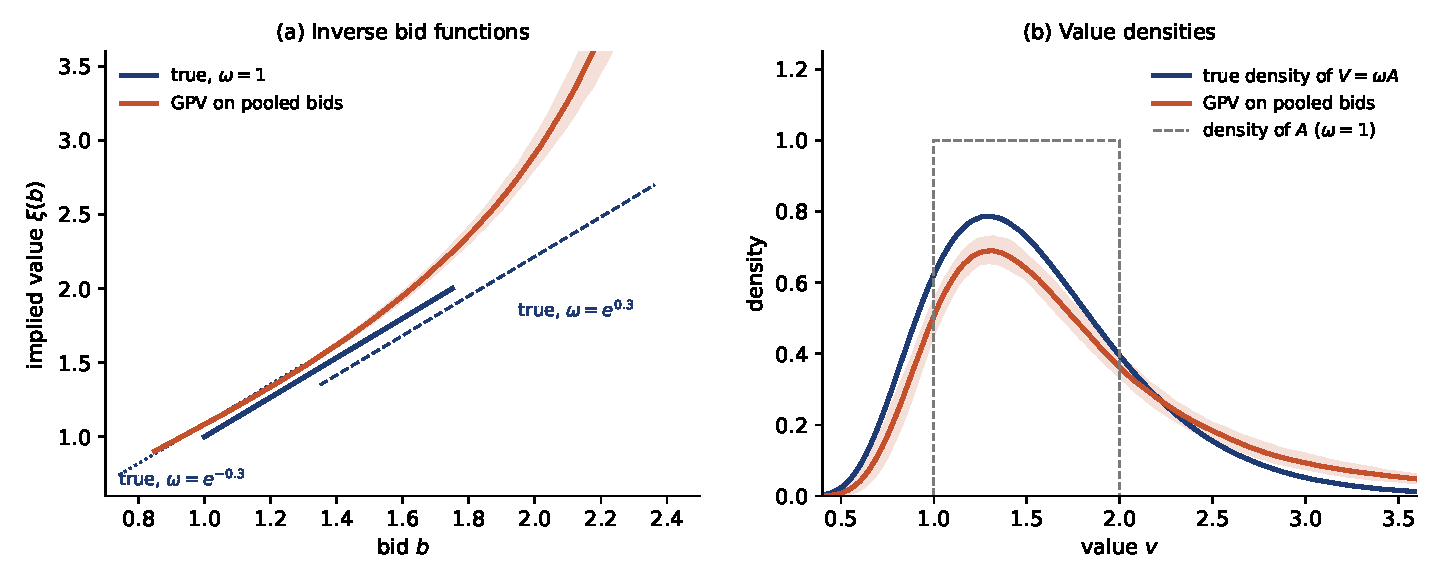
\includegraphics[width=\textwidth]{figures/ch15/uh_bias.pdf}
\caption{GPV applied to bids pooled across auctions with unobserved heterogeneity (our simulation,
seed 15701). Design of \cref{ex:15-uh-uniform}: $n=4$, $V=\omega A$, $A\sim U[1,2]$,
$\ln\omega\sim N(0,0.3^2)$, $T=500$ auctions, 200 samples. Panel (a): true inverse bid functions at
three values of $\omega$ and the median GPV estimate from pooled bids with a 5--95 percent band. Panel
(b): the true marginal density of $V$, the density of $A$ that bidders face at $\omega=1$, and the
median GPV estimate with its band. The true average markdown is $0.077$ and the median estimate is
$0.184$.}
\label{fig:15-uh-bias}
\end{figure}

\subsection{Separability and homogenization}\label{sec:15-uh-sep}

Equilibrium bidding inherits the additive or multiplicative structure of values. This property drives
every method in this section.

\begin{lemma}[Separability, after \citealp{AtheyHaile2007}, eqs. (6.4)--(6.5), and \citealp{Krasnokutskaya2011}, Proposition 1]\label{lem:15-separability}
Let \cref{ass:15-uh} hold with no binding reserve price. Let $(\alpha_1,\dots,\alpha_n)$ be the
equilibrium bid functions of the \emph{normalized game}, the game with $\omega=0$ in the additive case
and $\omega=1$ in the multiplicative case.
\begin{enumerate}[label=(\alph*)]
\item In a first-price auction with additive values, $\beta_i(v;\omega)=\omega+\alpha_i(v-\omega)$.
\item In a first-price procurement auction with multiplicative costs $C_i=\omega A_i$,
$\beta_i(c;\omega)=\omega\,\alpha_i\big(\frac{c}{\omega}\big)$. In a first-price auction with
multiplicative values $V_i=\omega A_i$, likewise $\beta_i(v;\omega)=\omega\,\alpha_i\big(\frac{v}{\omega}\big)$.
\item The \emph{homogenized bids} $B^0_{it}=B_{it}-\omega_t$ in case (a) and $B^0_{it}=\frac{B_{it}}{\omega_t}$
in case (b) equal $\alpha_i(A_{it})$. They are independent of $\omega_t$ and of each other, and they
have the bid distributions of the normalized game.
\end{enumerate}
\end{lemma}

\begin{proof}
We prove (b), the case used in the application below. Suppose bidders $j\neq i$ use
$\beta_j(c;\omega)=\omega\,\alpha_j\big(\frac{c}{\omega}\big)$ in the game with common component
$\omega$. A bidder with cost $C_j=\omega A_j$ then bids $\omega\,\alpha_j(A_j)$. Bidder $i$ wins with
bid $b$ when every rival bids more,
\[
\Pr\big(\text{$i$ wins}\mid b\big)=\Pr\big(\omega\,\alpha_j(A_j)>b\ \ \forall j\neq i\big)
=\Pr\Big(\alpha_j(A_j)>\frac{b}{\omega}\ \ \forall j\neq i\Big)\equiv P^0_i\Big(\frac{b}{\omega}\Big),
\]
where $P^0_i(a')$ is bidder $i$'s probability of winning with bid $a'$ in the normalized game. A bidder
with cost $c=\omega a$ who bids $b$ earns
\[
(b-\omega a)\,P^0_i\Big(\frac{b}{\omega}\Big)=\omega\Big(\frac{b}{\omega}-a\Big)P^0_i\Big(\frac{b}{\omega}\Big).
\]
Choosing $b$ is the same as choosing $a'=\frac{b}{\omega}$ to maximize $(a'-a)P^0_i(a')$. That is
bidder $i$'s problem in the normalized game, and its solution is $a'=\alpha_i(a)$. Hence the best
response is $b=\omega\,\alpha_i(a)=\omega\,\alpha_i\big(\frac{c}{\omega}\big)$, and the profile is an
equilibrium of the game with $\omega$. By \cref{ass:15-uh}(iii) it is the equilibrium. The sale
auction with $V_i=\omega A_i$ follows word for word, with $(v-b)$ in place of $(b-c)$ and win
probabilities $\Pr\big(\omega\,\alpha_j(A_j)<b\ \forall j\neq i\big)$. Part (a)
follows from the same argument with $b-\omega$ in place of $\frac{b}{\omega}$ and $(v-\omega)$ in place
of $a$. For (c), $B^0_{it}=\alpha_i(A_{it})$ is a function of $A_{it}$ alone, and the $A_{it}$ are
independent of $\omega_t$ and of each other.
\end{proof}

The argument needs the whole game to scale with $\omega$. A reserve price that does not move with
$\omega$ breaks it, which is one reason the application below relies on a nonbinding reserve. If the
number of bidders responds to $\omega_t$ through entry, part (c) holds only conditional on $n_t$, and
$n_t$ itself carries information about $\omega_t$.

\casehead{Homogenization with observed covariates}
Separability is useful even when all heterogeneity is observed. \Cref{sec:15-covariates} homogenized
transaction prices in ascending auctions, where bids equal values. \citet[Section 6.1.1]{AtheyHaile2007},
following \citet{HaileHongShum2003}, carry the idea over to first-price bids. Suppose, as in
\cref{thm:15-ah3}(ii), that $V_{it}=g_0(Z_t)+A_{it}$ with $A_{it}$ independent of $Z_t$ and the
normalization $g_0(z_0)=0$. \Cref{lem:15-separability}(a) with $\omega_t=g_0(Z_t)$ gives
$\beta_i(v;n,z)=g_0(z)+\beta_i\big(v-g_0(z);n,z_0\big)$. Bids therefore satisfy the regression
\begin{equation}\label{eq:15-homog-reg}
b_{it}=\kappa(n_t)+g_0(z_t)+\varepsilon_{it},\qquad
\varepsilon_{it}=\beta_i(V_{it}-g_0(z_t);n_t,z_0)-\kappa(n_t),\qquad \E[\varepsilon_{it}\mid z_t,n_t]=0,
\end{equation}
where $\kappa(n)$ is an intercept for $n$-bidder auctions, as in \cref{sec:15-covariates}. Ordinary least
squares on all bids estimates $g_0$. The homogenized bids $\hat b_{it}=b_{it}-\hat g_0(z_t)$ estimate
the bids that would have been placed at $z_0$. The GPV estimator applied to them, separately for each $n$,
recovers $F_V(\cdot;z_0)$, and then $F_V(v;z)=F_V\big(v-g_0(z);z_0\big)$ for every $z$. The first stage
uses all $\sum_nnT_n$ bids, so a flexible parametric $g_0$ converges at the parametric rate. As in the
ascending case, it leaves the nonparametric asymptotics of the second stage unchanged. The multiplicative
case works the same way in logs. \citet[eqs. (6.7)--(6.9)]{AtheyHaile2007} also describe sieve and finite-mixture
specifications of the bid distribution. These let covariates affect bids more flexibly, at the cost
of a priori structure, and covariate effects are then recovered only indirectly.

\casehead{Why unobserved heterogeneity needs more}
With $\omega_t$ unobserved, the analogue of \eqref{eq:15-homog-reg} is
$\ln b_{it}=\ln\omega_t+\ln B^0_{it}$. The term $\ln\omega_t$ is an auction fixed effect that cannot be
subtracted. The structure nevertheless suggests a remedy. Two bids from the same auction are two
noisy measurements of the same $\ln\omega_t$, with independent errors $\ln B^0_{it}$. This is the
repeated-measurement problem of the measurement-error literature \citep{LiVuong1998}, and
deconvolution solves it \citep[Section 6.1.2 and footnote 51]{AtheyHaile2007}.

\subsection{Identification by deconvolution: Krasnokutskaya (2011)}\label{sec:15-krasno}

\subsubsection{Question and model}

\citet{Krasnokutskaya2011} asks how much of the variation in contractors' costs is private
information, and how far IPV and APV estimators err when bidders share cost information that the
econometrician lacks. The answer matters for markups, for the efficiency of first-price
procurement, and for any policy evaluated with an estimated cost distribution. Her abstract states
that accounting for unobserved heterogeneity ``has important implications for the evaluation of the
distribution of rents, efficiency, and optimal auction design'' (p.~293). We cite the published
article by page. Some material appears only in the 2004 working paper \citep{Krasnokutskaya2004},
which we mark WP. Its application used a different sample and reported different headline numbers.
We give the published numbers and say where the WP figures differ.

There are $n$ bidders of two observable types, $n_1$ of type 1 and $n_2=n-n_1$ of type 2. Bidder
$i$'s cost of the project in auction $t$ is $C_{it}=\omega_tA_{it}$. The maintained assumptions
are the following (pp.~296--297).
\begin{enumerate}[label=(D\arabic*)]
\item $\omega_t,A_{1t},\dots,A_{nt}$ are mutually independent. $A_{it}$ has distribution $F_{k}$ for a
type-$k$ bidder, and the supports $[\underline\omega,\bar\omega]$ and $[\underline a,\bar a]$ lie in
$(0,\infty)$.
\item The densities $f_1,f_2$ are continuously differentiable and strictly positive on the interior
of the support.
\item $\E[A_{it}]=1$ for type-1 bidders.
\item The number of bidders is common knowledge, and there is no binding reserve price.
\end{enumerate}
(D1) is the identifying assumption. (D2) delivers existence and uniqueness of the equilibrium. (D3)
fixes the scale, since $(\omega,A)$ and $(c\,\omega,\frac{A}{c})$ produce the same costs. For each
$\omega$ the game is an asymmetric IPV procurement auction. Krasnokutskaya attributes the existence of a
unique equilibrium in strictly monotone, differentiable strategies to McAdams and others (p.~297). By
\cref{lem:15-separability}(b), $B_{it}=\omega_t\,\alpha_{k(i)}(A_{it})$, where $k(i)$ is bidder $i$'s
type. This is her Proposition 1, which she notes also holds for additive components (p.~298,
footnote 3).

Let $G^0_k$ and $g^0_k$ be the distribution and density of the homogenized bid $B^0=\alpha_k(A)$ of a
type-$k$ bidder, and write $-k$ for the other type. In the normalized game a type-$k$ bidder with cost
$a$ who bids $b^0$ wins with probability
$P^0_k(b^0)=\big(1-G^0_k(b^0)\big)^{n_k-1}\big(1-G^0_{-k}(b^0)\big)^{n_{-k}}$. Its first-order condition is
$P^0_k(b^0)+(b^0-a)P^{0\prime}_k(b^0)=0$, so that $a=b^0+\frac{P^0_k(b^0)}{P^{0\prime}_k(b^0)}$ with
\[
\frac{P^{0\prime}_k(b^0)}{P^0_k(b^0)}=-\frac{(n_k-1)\,g^0_k(b^0)}{1-G^0_k(b^0)}-\frac{n_{-k}\,g^0_{-k}(b^0)}{1-G^0_{-k}(b^0)} .
\]
Substituting gives the inverse bid function in terms of homogenized bid distributions (her eq. (1)
and condition (W6), pp.~298 and 302),
\begin{equation}\label{eq:15-krasno-inverse}
a=\xi_k(b^0)\equiv b^0-\frac{\big(1-G^0_k(b^0)\big)\big(1-G^0_{-k}(b^0)\big)}{(n_k-1)\,g^0_k(b^0)\big(1-G^0_{-k}(b^0)\big)+n_{-k}\,g^0_{-k}(b^0)\big(1-G^0_k(b^0)\big)} .
\end{equation}
This is the asymmetric procurement condition of \cref{sec:14-procurement}, applied to the normalized
game. It would identify $F_k$ immediately if homogenized bids were observed. They are not, because
$\omega_t$ is not.

\subsubsection{Kotlarski's lemma}

Deconvolution rests on a characterization result for sums of independent random variables. We write
$\mathrm i=\sqrt{-1}$ for the imaginary unit and $\varphi_Y(t)=\E\big[e^{\mathrm i tY}\big]$ for the
\emph{characteristic function} of a random variable $Y$ (\cref{app:math}).

\begin{lemma}[\citealp{Kotlarski1966}, and \citealp{AtheyHaile2007}, Lemma 6.1]\label{lem:15-kotlarski}
Let $Y_1,Y_2,Y_3$ be mutually independent random variables with finite means and characteristic
functions $\varphi_1,\varphi_2,\varphi_3$ that never vanish. Let $Q_1=Y_1+Y_3$ and $Q_2=Y_2+Y_3$, and let
$\Psi(t_1,t_2)=\E\big[e^{\mathrm i(t_1Q_1+t_2Q_2)}\big]$ be their joint characteristic function, with
partial derivative $\Psi_1$ in its first argument.
\begin{enumerate}[label=(\roman*)]
\item The joint distribution of $(Q_1,Q_2)$ determines the distributions of $Y_1,Y_2,Y_3$ up to
location.
\item Under the normalization $\E[Y_1]=0$,
\begin{equation}\label{eq:15-kotlarski}
\varphi_3(t)=\exp\Big(\int_0^t\frac{\Psi_1(0,u)}{\Psi(0,u)}\,du\Big),\qquad
\varphi_1(t)=\frac{\Psi(t,0)}{\varphi_3(t)},\qquad \varphi_2(t)=\frac{\Psi(0,t)}{\varphi_3(t)} .
\end{equation}
\end{enumerate}
\end{lemma}

\begin{proof}
\emph{Step 1.} By independence,
\[
\Psi(t_1,t_2)=\E\big[e^{\mathrm it_1Y_1}\,e^{\mathrm it_2Y_2}\,e^{\mathrm i(t_1+t_2)Y_3}\big]
=\varphi_1(t_1)\,\varphi_2(t_2)\,\varphi_3(t_1+t_2).
\]
\emph{Step 2.} Finite means make each $\varphi_j$ differentiable, with $\varphi_j'(0)=\mathrm i\,\E[Y_j]$.
Differentiating in $t_1$,
\[
\Psi_1(t_1,t_2)=\varphi_1'(t_1)\varphi_2(t_2)\varphi_3(t_1+t_2)+\varphi_1(t_1)\varphi_2(t_2)\varphi_3'(t_1+t_2).
\]
\emph{Step 3.} At $t_1=0$, use $\varphi_1(0)=1$ and $\varphi_1'(0)=\mathrm i\,\E[Y_1]=0$:
\[
\Psi_1(0,u)=\varphi_2(u)\,\varphi_3'(u),\qquad \Psi(0,u)=\varphi_2(u)\,\varphi_3(u).
\]
\emph{Step 4.} Since $\varphi_2(u)\neq0$, dividing gives
$\frac{\Psi_1(0,u)}{\Psi(0,u)}=\frac{\varphi_3'(u)}{\varphi_3(u)}$. Let
$L(t)=\int_0^t\frac{\varphi_3'(u)}{\varphi_3(u)}du$. Then
\[
\frac{d}{dt}\Big[\varphi_3(t)e^{-L(t)}\Big]=e^{-L(t)}\Big(\varphi_3'(t)-\varphi_3(t)\frac{\varphi_3'(t)}{\varphi_3(t)}\Big)=0,
\]
and $\varphi_3(0)e^{-L(0)}=1$. Hence $\varphi_3(t)=e^{L(t)}$, the first formula in \eqref{eq:15-kotlarski}.
\emph{Step 5.} Setting $t_2=0$ and then $t_1=0$ in Step 1 gives $\Psi(t,0)=\varphi_1(t)\varphi_3(t)$ and
$\Psi(0,t)=\varphi_2(t)\varphi_3(t)$, which yield the other two formulas.
\emph{Step 6.} A characteristic function determines its distribution (L\'evy's inversion theorem),
which proves (ii). Without the normalization, Step 3 adds $\mathrm i\,\E[Y_1]$ to the ratio, so
$\varphi_3$ is recovered up to the factor $e^{\mathrm it\E[Y_1]}$. Adding a constant to $Y_3$ and
subtracting it from $Y_1$ and $Y_2$ leaves $(Q_1,Q_2)$ unchanged, which proves (i).
\end{proof}

The proof uses Step 4 to avoid taking logarithms of a complex function. The idea is simple. With two
measurements sharing one component, the covariation of $Q_1$ and $Q_2$ isolates the shared part, and
the marginals then reveal the rest.

\begin{example}[Normal components]\label{ex:15-kotlarski-normal}
Let $Y_1\sim N(0,\sigma_1^2)$, $Y_2\sim N(\mu_2,\sigma_2^2)$ and $Y_3\sim N(\mu_3,\sigma_3^2)$. Then
\[
\ln\Psi(t_1,t_2)=\mathrm i\mu_2t_2+\mathrm i\mu_3(t_1+t_2)-\tfrac{1}{2}\big[\sigma_1^2t_1^2+\sigma_2^2t_2^2+\sigma_3^2(t_1+t_2)^2\big],
\]
so $\frac{\Psi_1(0,u)}{\Psi(0,u)}=\mathrm i\mu_3-\sigma_3^2u$. Integrating from $0$ to $t$ gives
$\varphi_3(t)=\exp\big(\mathrm i\mu_3t-\frac{1}{2}\sigma_3^2t^2\big)$, the $N(\mu_3,\sigma_3^2)$
characteristic function. Here $\sigma_3^2=\Cov(Q_1,Q_2)$ and $\mu_3=\E[Q_1]$. In the normal case means
and covariances suffice. In general the lemma uses the entire joint distribution of the two
measurements.
\end{example}

\subsubsection{Identification}

\begin{theorem}[\citealp{Krasnokutskaya2011}, Theorem 1]\label{thm:15-krasno}
Let (D1)--(D4) hold with $n_1\ge1$ and $n_2\ge1$, and suppose the characteristic functions of $\ln\omega$ and
of $\ln B^0$ for each type never vanish.
\begin{enumerate}[label=(\roman*)]
\item The joint distribution of the bids $(B_{i_1t},B_{i_2t})$ of a type-1 and a type-2 bidder in the same
auction identifies $F_\omega$, $F_1$ and $F_2$.
\item The joint distribution of two bids of type-$k$ bidders in the same auction identifies $F_\omega$ and
$G^0_k$ up to a common scale. Together with the marginal distribution of one bid of the other type, it
identifies $F_\omega$, $F_1$ and $F_2$.
\end{enumerate}
\end{theorem}

\begin{proof}
\emph{Step 1 (separate the common component).} Let bidder $i_1$ have type 1 and bidder $i_2$ type 2. By
\cref{lem:15-separability}(b),
\[
\ln B_{i_1t}=\ln\omega_t+\ln B^0_{i_1t},\qquad \ln B_{i_2t}=\ln\omega_t+\ln B^0_{i_2t},
\]
with $\ln\omega_t$, $\ln B^0_{i_1t}=\ln\alpha_1(A_{i_1t})$ and $\ln B^0_{i_2t}=\ln\alpha_2(A_{i_2t})$
mutually independent by (D1). Bounded supports give finite means. Apply \cref{lem:15-kotlarski} with
$Y_3=\ln\omega$, $Y_1=\ln B^0_1$ and $Y_2=\ln B^0_2$, under the location normalization
$\E[\ln B^0_1]=0$. The distributions of $\ln\omega$, $\ln B^0_1$ and $\ln B^0_2$ are identified, and
since the logarithm is strictly increasing, so are $F_\omega$, $G^0_1$ and $G^0_2$.

\emph{Step 2 (invert the normalized game).} With $G^0_1,G^0_2$ and their densities known,
\eqref{eq:15-krasno-inverse} identifies $\xi_1$ and $\xi_2$. These are strictly increasing in
equilibrium, so $F_k(a)=G^0_k\big(\xi_k^{-1}(a)\big)$, as in \citet{LaffontVuong1996} for asymmetric
IPV.

\emph{Step 3 (impose the scale).} The location normalization in logs is a scale normalization in
levels. Rescaling all homogenized bids by $c$ rescales $\xi_k$, and hence $A$, by $c$, and rescales
$\omega$ by $\frac{1}{c}$. The unique $c$ with $\E[A]=1$ for type 1 implements (D3). This proves (i).

\emph{Step 4 (a same-type pair).} For (ii), apply \cref{lem:15-kotlarski} to the two type-$k$ log bids under the
normalization $\E[\ln B^0_k]=0$. This identifies the distributions of $\ln\omega$ and $\ln B^0_k$ up to a common
location in logs, which is a common scale in levels. The pair carries no information about the other type, and
\eqref{eq:15-krasno-inverse} for either type involves both $G^0_1$ and $G^0_2$, since $n_1\ge1$ and $n_2\ge1$.
A bid of the other type satisfies $\ln B_{-k}=\ln\omega+\ln B^0_{-k}$ with independent terms, so
$\varphi_{\ln B^0_{-k}}=\frac{\varphi_{\ln B_{-k}}}{\varphi_{\ln\omega}}$, which is well defined because
$\varphi_{\ln\omega}$ never vanishes. Its marginal distribution therefore identifies $G^0_{-k}$ on the same scale.
Steps 2 and 3 then apply unchanged.
\end{proof}

Several remarks qualify the result. First, realizations are not identified. The $n$ bids of an
auction are $n$ equations in the $n+1$ unknowns $\omega_t,A_{1t},\dots,A_{nt}$ (p.~300). Distributions
are identified, but no individual cost is. Second, a single bid per auction would not suffice. The
distribution of $\ln B=\ln\omega+\ln B^0$ alone has many decompositions into independent parts. Third,
the nonvanishing condition is taken from \citet[Lemma 6.1]{AtheyHaile2007}. Krasnokutskaya's appendix
argues instead that bounded supports make the characteristic functions entire, so that their zeros
form a countable set (p.~320, Lemma A1). Fourth, the theorem makes the data requirement more explicit than the
source does. Krasnokutskaya writes that any pair of bids identifies $F_\omega$, and that $F_k$ is identified from any
pair that contains a type-$k$ bidder (p.~299). For a same-type pair this needs part (ii). The inverse
\eqref{eq:15-krasno-inverse} depends on the other type's bid distribution, and (D3) fixes the scale through
type 1, which a pair of type-2 bids does not reveal. Her data contain every bid of each auction, so the
marginal of the other type is available and the qualification does not affect the application. In auctions
whose bidders all have one type, the inverse involves that type alone. A same-type pair then identifies $F_\omega$
and $F_k$ once the scale is normalized on that type.

\subsubsection{Testable restrictions and extensions}

The model has overidentifying content when three or more bids are observed (Section 3.2). Ratios of
bids eliminate $\omega_t$,
\[
\ln\frac{B_{i_1t}}{B_{i_3t}}=\ln B^0_{i_1t}-\ln B^0_{i_3t},\qquad
\ln\frac{B_{i_2t}}{B_{i_3t}}=\ln B^0_{i_2t}-\ln B^0_{i_3t}.
\]
Now $-\ln B^0_{i_3t}$ plays the role of the common component. Applying \cref{lem:15-kotlarski} to the
ratios uses only independence across bidders, and not independence of $\omega$ and $\bm A$. Her
Proposition 2 lists three implications. (W1) If bidders $i_1$ and $i_3$ have the same type, the
distributions of $\ln B^0_{i_1}$ and $\ln B^0_{i_3}$ recovered from the ratios coincide. (W2) The
distributions recovered from the ratios coincide with those recovered from the pair
$(\ln B_{i_1},\ln B_{i_2})$, which holds only if $\omega$ is independent of $\bm A$. (W3) For four
distinct bidders, $\frac{B_{i_1}}{B_{i_2}}$ and $\frac{B_{i_3}}{B_{i_4}}$ are independent. Independence
of the private components implies (W1) and (W3), and independence of $\omega$ and $\bm A$ adds (W2)
(pp.~301--302). (W1) and (W2) need three bids per auction, and (W3) needs four.

Her Proposition 3 collects restrictions that every model with unobserved heterogeneity imposes on the
data (p.~302). (W4) The functions in \eqref{eq:15-kotlarski} are characteristic functions of real
random variables, and the two individual components they describe have the same support. (W5) They do
not depend on which pair of bidders is used. (W6) Each $\xi_k$ in \eqref{eq:15-krasno-inverse} is
strictly increasing, the restriction that \citet{GuerrePerrigneVuong2000} pointed out without
heterogeneity. If a model with unobserved heterogeneity generated the data, (W4)--(W6) hold. The WP
also presents them as sufficient. It adds that a degenerate distribution of $\ln\omega$, its condition
(W7), marks IPV data (WP, Proposition 4).

Two limits of the result deserve emphasis. The first concerns APV. Both models make bids in the same
auction dependent, but heterogeneity makes them conditionally independent, while APV makes them
affiliated. By results related to de Finetti's theorem, the set of affiliated distributions is larger
than the set of conditionally independent ones. Some APV bid distributions therefore cannot come from
unobserved heterogeneity (p.~302). Restriction (W3) gives a practical test. Under heterogeneity,
ratios of distinct pairs of bids from the same auction are independent. Many APV distributions violate
this, among them the truncated multivariate normal for a large set of parameters (p.~303). The
test has no power against a small set of affiliated distributions. The WP took a different view. It
conjectured that heterogeneity with affiliated components is not identified, and it read the
heterogeneity model as attributing the least private information consistent with the data (WP,
Section 6). Second, the multiplicative form ties the mean and the dispersion of costs together. The
extension $C_{it}=\omega_{1t}+\omega_{2t}A_{it}$, with independent $\omega_1$, $\omega_2$ and $\bm A$,
lets the two vary separately. The WP's Theorem 1a identifies all distributions from four bids per
auction. Kotlarski's argument is applied to the logs of differences of bids to recover the scale
component $\omega_2$, and then to differences and levels to recover the rest (WP, Appendix A). The
published article leaves this model to a separate note by the author (p.~319).

\subsubsection{Estimation}

The estimator follows the proof (Section 4.1 and Appendix A.2). Estimation is carried out within a
cell of auctions with the same $(n,n_1)$ and the same discrete covariates. Let $T_0$ be the number of
auctions in the cell.

\casehead{Step 1: deconvolution}
The joint characteristic function of a type-1 and a type-2 log bid and its derivative are estimated
by averages over auctions and over all such pairs of bidders,
\begin{align*}
\hat\Psi(t_1,t_2)&=\frac{1}{T_0}\sum_{t=1}^{T_0}\frac{1}{n_1n_2}\sum_{i:\,k(i)=1}\ \sum_{j:\,k(j)=2}
e^{\mathrm i(t_1\ln b_{it}+t_2\ln b_{jt})},\\
\hat\Psi_1(t_1,t_2)&=\frac{1}{T_0}\sum_{t=1}^{T_0}\frac{1}{n_1n_2}\sum_{i:\,k(i)=1}\ \sum_{j:\,k(j)=2}
\mathrm i\ln b_{it}\;e^{\mathrm i(t_1\ln b_{it}+t_2\ln b_{jt})}.
\end{align*}
Plugging these into \eqref{eq:15-kotlarski} gives $\hat\varphi_{\ln\omega}$, $\hat\varphi_{\ln B^0_1}$
and $\hat\varphi_{\ln B^0_2}$. Densities follow from a truncated inverse Fourier transform with the
damping factor of \citet{DiggleHall1993} and \citet{LiPerrigneVuong2000},
\begin{equation}\label{eq:15-damped-inverse}
\hat f_{\ln\omega}(y)=\frac{1}{2\pi}\int_{-T_c}^{T_c}\Big(1-\frac{|t|}{T_c}\Big)e^{-\mathrm ity}\,\hat\varphi_{\ln\omega}(t)\,dt,
\end{equation}
and likewise for $\ln B^0_k$. We call the truncation constant $T_c$ to keep $T$ for the number of
auctions. A change of variables gives $\hat f_\omega(w)=\frac{1}{w}\hat f_{\ln\omega}(\ln w)$. The damping
factor tames the oscillating tails that truncation produces (pp.~324--325). She chooses $T_c$ by
matching the first two moments of each component (p.~325). The targets come from a type-1 and a
type-2 log bid in the same auction. Under the normalization $\E[\ln B^0_1]=0$ they are
\begin{align*}
\E[\ln\omega]&=\E[\ln B_1],\\
\Var(\ln\omega)&=\frac{1}{2}\big[\Var(\ln B_1)+\Var(\ln B_2)-\Var(\ln B_1-\ln B_2)\big]=\Cov(\ln B_1,\ln B_2),
\end{align*}
together with $\E[\ln B^0_2]=\E[\ln B_2]-\E[\ln B_1]$ and $\Var(\ln B^0_k)=\Var(\ln B_k)-\Var(\ln\omega)$
(p.~325, footnote 34). For each candidate $T_c$ she computes the moments of the estimated densities and
picks the $T_c$ that minimizes the squared deviations from the targets, scaled by the target variances.
In the application this gives $T_c=50$ (p.~325). Support bounds are estimated from the extremes of log
bids and of differences of log bids (p.~321). A bias correction of the kind proposed by Horowitz
and Markatou improves small-sample performance (p.~304, footnote 15, and p.~325). The WP also rescales bids into $[0,2\pi]$ before
estimation (WP, pp.~16--17).

\casehead{Step 2: inversion}
Let $\hat{\underline b}^0_k$ be the estimated lower end of the support of type-$k$ homogenized bids. With
$\hat g^0_k$ and $\hat G^0_k(b^0)=\int_{\hat{\underline b}^0_k}^{b^0}\hat g^0_k$ in hand, evaluate
\eqref{eq:15-krasno-inverse} on a grid of homogenized bids to obtain $\hat\xi_k$ (p.~304, Step 6).
Invert it to get the normalized bid function $\hat\alpha_k=\hat\xi_k^{-1}$. The distribution of the
private component is then
\[
\hat F_k(a)=\hat G^0_k\big(\hat\xi_k^{-1}(a)\big),
\]
the sample analogue of Step 2 of the proof (Steps 7--8). Finally, rescale so that $\E[A]=1$ for type 1
(Step 9). The WP instead drew pseudo homogenized bids from $\hat g^0_k$, computed pseudo costs
$\hat\xi_k(\tilde b^0_\ell)$, and smoothed them with the triweight kernel
$\mathcal K(u)=\frac{35}{32}(1-u^2)^3\indic(|u|\le1)$. Its bandwidth was
$2.978\times1.06\,\hat\sigma\,L^{-\frac{1}{6}}$, with $\hat\sigma$ the standard deviation of
$\ln(1+\text{bids})$ (WP, p.~17).

Two derived objects summarize the results (p.~305, Steps 10--11). The density of total cost is
$f_{C_k}(c)=\int f_k\big(\frac{c}{u}\big)\frac{1}{u}f_\omega(u)\,du$. The \emph{expected inverse bid
function} is the expected cost of a type-$k$ bidder who submits the bid $b$,
$\bar\xi_k(b)=\E[C_k\mid B_k=b]$. Since $C_k=\omega\,\xi_k(B^0_k)$ and $B_k=\omega B^0_k$,
\[
\bar\xi_k(b)=\int u\,\xi_k\Big(\frac{b}{u}\Big)f_\omega(u\mid b)\,du,\qquad
f_\omega(u\mid b)=\frac{f_\omega(u)\,g^0_k\big(\frac{b}{u}\big)\frac{1}{u}}{\int f_\omega(y)\,g^0_k\big(\frac{b}{y}\big)\frac{1}{y}\,dy}.
\]
The weight is the posterior density of $\omega$ given $B_k=b$. By Bayes' rule it multiplies the prior
$f_\omega(u)$ by the density $\frac{1}{u}g^0_k(\frac{b}{u})$ of the bid given $\omega=u$. This likelihood
vanishes outside $\frac{b}{\bar b^0_k}\le u\le\frac{b}{\underline b^0_k}$, where $[\underline b^0_k,\bar b^0_k]$
is the support of the homogenized bids of type $k$. Krasnokutskaya's Step 11 instead weights by the prior
truncated to this interval (p.~305, footnote 16). That weight omits the likelihood inside the interval, so it
does not deliver $\E[C_k\mid B_k=b]$ in general. Take two symmetric bidders with $A$ uniform on
$[\frac12,\frac32]$ and $\omega$ uniform on $[1,2]$, for example. The bid function is $\frac{a}{2}+\frac34$, so
homogenized bids are uniform on $[1,\frac32]$. At $b=\frac32$ the posterior mean of $\omega$ is
$\frac{1}{2\ln1.5}\approx1.233$ and $\E[C\mid B=b]\approx1.150$. The truncated prior gives $1.25$ and $1.125$.

\casehead{Properties}
Her Proposition 4 shows that $\hat F_\omega$ and $\hat F_k$ are uniformly consistent under (D1)--(D4) and
(D5) (p.~305). Condition (D5) requires the characteristic functions of $\ln\omega$ and $\ln B^0_k$ to
be \emph{ordinary smooth} of order $\varkappa>1$ in the sense of \citet{Fan1991}, that is,
$d_0|t|^{-\varkappa}\le|\varphi(t)|\le d_1|t|^{-\varkappa}$ as $|t|\to\infty$. The rate for the
deconvolved densities is taken from \citet{LiVuong1998} (p.~322). Deconvolution estimators converge
slowly, so large samples are needed \citep[Section 6.1.2]{AtheyHaile2007}. Confidence intervals come
from the bootstrap (p.~305).

\Cref{fig:15-kotlarski} shows the estimator at work in a simulation of our own. Two features stand
out. Pairs of bids recover two distributions with opposite skewness that a single bid would blur into
one symmetric-looking density. The bands are wide even with 1,000 auctions and four bids each, which
illustrates the slow rates.

\begin{figure}[htbp]
\centering
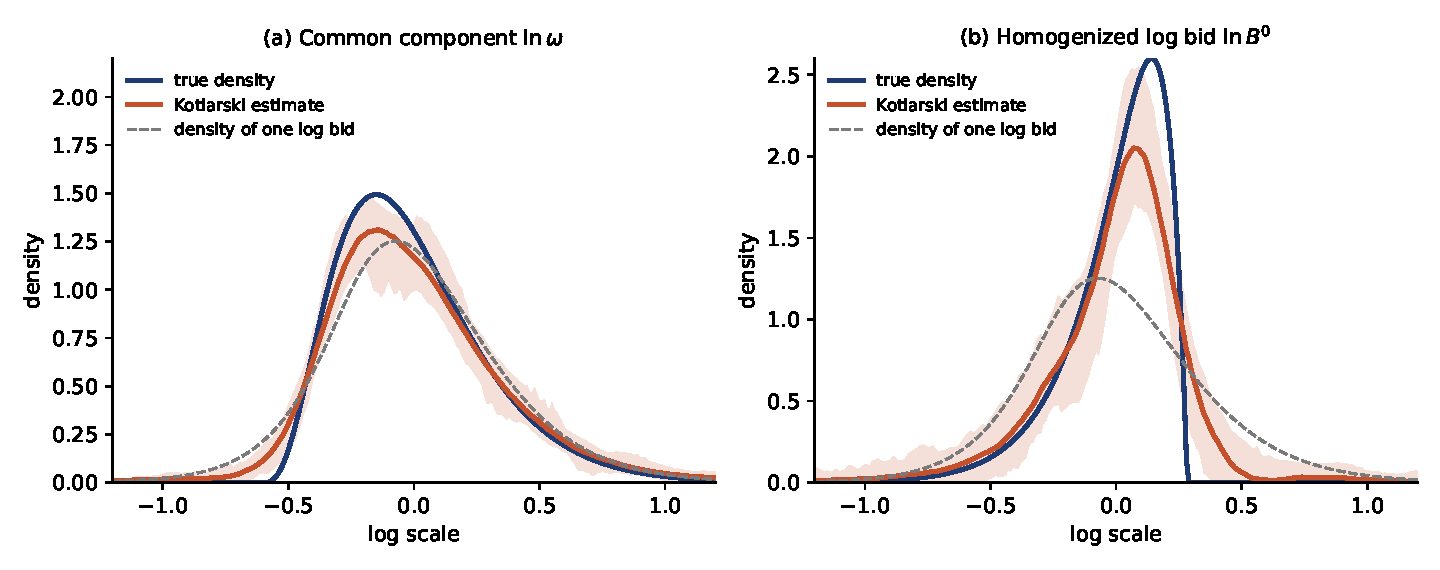
\includegraphics[width=\textwidth]{figures/ch15/kotlarski_demo.pdf}
\caption{Deconvolution of log bids with \eqref{eq:15-kotlarski} and the damped inverse
\eqref{eq:15-damped-inverse} (our simulation, seed 15703). $T=1{,}000$ auctions with four bidders of
one type. $\ln\omega$ is a standardized $\text{Gamma}(4)$ variable scaled to standard deviation $0.3$,
and $\ln B^0$ is a reflected standardized $\text{Gamma}(2)$ variable scaled to standard deviation
$0.2$. Characteristic functions average over all ordered pairs of bids. $T_c$ is chosen by
Krasnokutskaya's moment criterion on the grid $3,4,\dots,25$, and the largest value is usually chosen.
Lines show the median over 200 samples, bands the 5--95 percent range. The dashed curve is the density
of a single log bid.}
\label{fig:15-kotlarski}
\end{figure}

\subsubsection{Monte Carlo evidence}

The published Monte Carlo study is reported in figures only (Section 4.3, pp.~306--309). Costs are
multiplicative, $C=\omega A$, with distributions shaped like the estimated ones. Each sample has two
bidders of each type, as in the data, and $T=250$, $200$ or $150$ auctions, so each private component
is estimated from 500, 400 or 300 bids. The 5--95 percent bands of the estimated distributions
contain the true ones except in the smallest samples, where the bands are wide and miss small parts
of the true functions (p.~306).

The WP ran a more detailed study with tables, which we report next. Its design is additive,
$C=\omega+A$, with symmetric bidders (WP, Section 4.4). $A$ is
uniform with mean zero and variance $0.33$. $\omega$ follows a power distribution with exponent 3 and
mean $10.5$, with variances chosen so that bid functions have closed forms. Each sample has $T=400$
auctions with two bidders, and each experiment is replicated 500 times. Five cases are studied (WP,
Table 1b). Case 1 has independent costs. Case 2 has unobserved heterogeneity with $\Var(\omega)=0.04$
or $0.34$. Case 3 is APV, with bidders who observe only $C$. Cases 4 and 5 add correlation among
private components or between private and common components.
The estimator behaves as theory predicts (WP, Table 2b). With independent costs the estimated
$\Var(\omega)$ is $0.013$, with interval $[0.01,0.02]$, close to degenerate. The estimated markup is
$0.362$ against a true $0.38$. With heterogeneity, the estimated variances of $A$ are $0.321$ and $0.318$
against $0.33$. The estimated variances of $\omega$ are $0.0362$ and $0.335$ against $0.04$ and $0.34$.
Markups are $0.082$ and $0.092$ against $0.09$. WP Table 3b prints a true markup of $0.03$ for
$\Var(\omega)=0.34$, so the two tables of the paper disagree (see the notes to
\cref{tab:15-krasno-mc}). With APV data the procedure misreads the information
structure. The estimated markup is $0.18$ against a true $0.47$ in case 3a, and $0.33$ against $0.21$
in case 3b. With correlated components, the variance of $\omega$ is overstated and that of $A$
understated. The bias is negligible when the correlation is about 5 percent of $\Var(A)$ (WP, pp.
19--20).

The second experiment applies IPV and APV estimators to data with heterogeneity.
\Cref{tab:15-krasno-mc} reproduces the results. As $\Var(\omega)$ grows, both misspecified procedures
understate mean costs, overstate their variance, and overstate markups. Krasnokutskaya reports that the
bias becomes significant once the correlation of costs reaches about $0.3$ (WP, p.~21). Their bid
functions are flatter than the truth, and the IPV estimate is especially flat at the low end. A known
common component produces a bid distribution with thin tails, which IPV reads as extreme shading
at the bottom.

\begin{table}[htbp]
\centering
\caption{Misspecified estimators applied to data with unobserved heterogeneity (Krasnokutskaya 2004
working paper, Table 3b, not in the published article)}
\label{tab:15-krasno-mc}
\begin{tabular}{llccc}
\toprule
$\Var(\omega)$ & Procedure & $\E(C)$ & $\Var(C)$ & $\E(\text{markup})$\\
\midrule
0.04 & True model & 10.5 & 0.37 & 0.09\\
     & UH  & [10.44, 10.59] & [0.32, 0.41] & [0.078, 0.095]\\
     & APV & [10.37, 10.48] & [0.35, 0.44] & [0.097, 0.12]\\
     & IPV & [10.41, 10.5]  & [0.34, 0.44] & [0.95, 0.11]\\
\addlinespace
0.34 & True model & 10.5 & 0.67 & 0.03\\
     & UH  & [10.28, 10.64] & [0.63, 0.72] & [0.02, 0.038]\\
     & APV & [8.31, 9.57]   & [0.89, 1.02] & [0.042, 0.55]\\
     & IPV & [8.85, 9.84]   & [0.83, 0.96] & [0.4, 0.52]\\
\addlinespace
1    & True model & 10.5 & 1.33 & 0.01\\
     & UH  & [10.15, 10.76] & [1.27, 1.43] & [0.008, 0.014]\\
     & APV & [7.6, 8.8]     & [2.01, 2.27] & [0.033, 0.047]\\
     & IPV & [8.1, 9.2]     & [1.86, 2.05] & [0.31, 0.044]\\
\bottomrule
\end{tabular}

\smallskip
\begin{minipage}{0.93\textwidth}
\footnotesize \textit{Notes.} Additive design $C=\omega+A$, two symmetric bidders, 400 auctions, 500
replications. UH, APV and IPV denote estimators that assume unobserved heterogeneity, affiliated
private values and independent private values. Brackets give 5th and 95th pointwise percentiles of
the estimator. Entries are reproduced as printed. Four markup intervals look like decimal-point
typos in the source: $[0.95,0.11]$, $[0.042,0.55]$, $[0.4,0.52]$ and $[0.31,0.044]$. The true markup
at $\Var(\omega)=0.34$ is printed as $0.03$ here and as $0.09$ in WP Table 1b.
\end{minipage}
\end{table}

\subsubsection{Application: Michigan highway maintenance}

\casehead{Setting}
The Michigan Department of Transportation allocates road work by first-price sealed-bid auctions
(Section 5.1, pp.~306--307). It advertises a project 4 to 10 weeks before the letting, with a short
description of location, completion time and tasks. Firms can obtain a detailed description. The
department prepares an \emph{engineer's estimate} from the work required for each task, priced with
winning bids on similar past projects and deflated. Federal law requires the winning bid to be below
110 percent of this estimate, unless the state justifies an exception in writing. Bids and even
winning bids above the threshold appear in the data, so Krasnokutskaya treats the reserve as
nonbinding. Following the literature, she assumes bidders know how many rivals they face
(pp.~309--310).

\casehead{Data}
The sample covers maintenance projects with bituminous resurfacing as the main task, let between
February 1997 and December 2003, a total of 3,947 projects (p.~310). For each project she observes the
letting date, completion time, location, tasks, the identities and bids of all bidders, and the
engineer's estimate. Two arguments support the model. Resurfacing jobs are precisely specified and
simple, which favors private values. Their costs depend on elevation, curvature, traffic and the age
of the surface, which contractors see on site visits and the researcher does not. Firms differ mainly
in size, which every participant observes, so she allows two observable types. A bidder is
\emph{regular} if it won at least \$10 million of projects in each year of the data and has at least
100 employees (p.~310). She notes that this matches the industry's definition of a large bidder
(footnote 19). All other bidders are \emph{fringe}. The WP used a different definition, which the
published one replaces. There a regular bidder submits at least 12 bids per year, ranks in the top 10
percent of firms by employment and works in three or more specializations (WP, Section 5.2).

The number of bidders ranges from 1 to 11. More than 85 percent of projects have 2 to 6 bidders, and
the mean is 3.4 with standard deviation 1.3. About 75 percent of engineer's estimates lie between
\$100,000 and \$1,000,000, with 5 percent below and 20 percent above (p.~310).
\Cref{tab:15-krasno-desc} reproduces her descriptive table. The gap between the estimate and the
winning bid grows with the number of bidders. \emph{Money left on the table} is the gap between the two
lowest bids relative to the estimate. It averages 7 percent and falls from 11 to 4 percent as the
number of bidders rises (p.~311).

\begin{table}[htbp]
\centering
\caption{Michigan highway maintenance auctions: descriptive statistics by number of bidders
(Krasnokutskaya 2011, Table 1, and WP Table 1c)}
\label{tab:15-krasno-desc}
\begin{tabular}{lccccccc}
\toprule
Number of bidders & Overall & 1 & 2 & 3 & 4 & 5 & 6\\
\midrule
Number of observations & 3,947 & 71 & 673 & 1,126 & 1,026 & 365 & 192\\
\addlinespace
Engineer's estimate & 12.80 & 13.34 & 10.27 & 12.60 & 13.90 & 12.90 & 16.40\\
 & (2.35) & (2.88) & (1.41) & (3.02) & (2.26) & (1.79) & (3.39)\\
Winning bid & 11.10 & 14.12 & 10.00 & 11.80 & 12.90 & 11.80 & 15.20\\
 & (2.32) & (3.05) & (1.50) & (2.89) & (2.25) & (1.66) & (3.35)\\
Money left on the table & 0.07 & NA & 0.11 & 0.08 & 0.07 & 0.05 & 0.04\\
 & (0.05) & NA & (0.08) & (0.06) & (0.06) & (0.05) & (0.04)\\
Number of regular bidders & 1.92 & 0.79 & 1.43 & 1.65 & 2.07 & 2.16 & 2.29\\
 & (1.06) & (0.41) & (0.62) & (0.72) & (0.98) & (1.21) & (1.32)\\
\bottomrule
\end{tabular}

\smallskip
\begin{minipage}{0.93\textwidth}
\footnotesize \textit{Notes.} Means with standard deviations in parentheses. The engineer's estimate and the
winning bid are in hundreds of thousands of dollars. Money left on the table is the difference
between the lowest and second-lowest bids divided by the engineer's estimate. The overall column
includes projects with 7 to 11 bidders. The published Table 1 prints the columns for 2 to 6 bidders as
shown. Its overall column is misprinted, with 1.175 and 4.660 in every row, and its one-bidder column
prints the overall values. We take these two columns from WP Table 1c.
\end{minipage}
\end{table}

\casehead{Evidence of heterogeneity}
Krasnokutskaya first tests for heterogeneity (Section 5.2, p.~311). She conditions on a linear index
of observables estimated by ordinary least squares. The index contains the engineer's estimate,
duration, highway type, year, month and district dummies, and the number of tasks. The tests run
within cells defined by the main task and the number of bidders (Appendix A.3). The first test asks
whether two bids from the same auction are independent given the index, which is the null of IPV
against heterogeneity. The second asks whether two ratios built from four distinct bids are
independent, restriction (W3). This is the null of heterogeneity against APV. For resurfacing
projects with four regular bidders, the $p$-values are 0.03 and 0.52. IPV is rejected at the 5 percent
level, and heterogeneity is not rejected against APV. The test sample has 370 auctions with
estimates between \$350,000 and \$750,000 (footnote 21). \Cref{tab:15-krasno-index} reproduces the
index regressions.

\begin{table}[htbp]
\centering
\caption{Linear index of log bids on observables (Krasnokutskaya 2011, Table 2)}
\label{tab:15-krasno-index}
\begin{tabular}{lcc}
\toprule
 & Test subsample & Estimation subsample\\
\midrule
Constant & 0.375 & 0.327\\
 & (0.010) & (0.012)\\
Engineer's estimate & 0.8413 & 0.8113\\
 & (0.028) & (0.025)\\
Duration & 0.0011 & 0.0015\\
 & (0.0013) & (0.0011)\\
Tasks & 0.0014 & 0.0012\\
 & (0.0007) & (0.0009)\\
\addlinespace
$(n_{\text{regular}},n_{\text{fringe}})$ & (4,0) & (2,2)\\
Number of projects & 370 & 226\\
$R^2$ & 33\% & 17\%\\
\bottomrule
\end{tabular}

\smallskip
\begin{minipage}{0.8\textwidth}
\footnotesize \textit{Notes.} Ordinary least squares estimates of the mean of the log bid, with the figures in
parentheses as printed. Variables are labeled as in the source, which does not say whether the
engineer's estimate enters in logs. The test subsample is used for the specification tests and the
estimation subsample for the deconvolution.
\end{minipage}
\end{table}

The WP looked at the same correlation more directly. Its regressions of log bids in four-bidder
resurfacing projects are reproduced in \cref{tab:15-krasno-bids} (WP, Table 2c). Bids rise with the
engineer's estimate, distance to the site and the firm's backlog (``load remaining''), and fall with
the number of potential bidders. Fringe firms bid more. Adding auction dummies raises $R^2$ from
$0.857$ to $0.914$. The random-effects estimates attribute $\rho=0.48$ of the residual variance of log
bids to the auction level. The printed variance components imply a smaller share,
$\frac{0.16}{0.16+0.22}\approx0.42$. The text reports $R^2$ values of $0.81$ and $0.89$ for the same
regressions (WP, p.~25), which also differ from the table.
Common variation across bids in an auction that observables do not explain is the signature of
unobserved heterogeneity.

\begin{table}[htbp]
\centering
\caption{Regressions of log bids, four-bidder resurfacing projects (Krasnokutskaya 2004 working
paper, Table 2c, selected rows)}
\label{tab:15-krasno-bids}
\begin{tabular}{lccc}
\toprule
 & OLS & Auction dummies & Random effects\\
\midrule
Log (estimate) & 0.9100 & 0.9300 & 0.8800\\
 & (0.0530) & (0.1400) & (0.1300)\\
Duration & $-0.0210$ & $-0.0490$ & $-0.0210$\\
 & (0.0500) & (0.0250) & (0.0500)\\
Distance & 0.0312 & 0.0540 & 0.0270\\
 & (0.0160) & (0.0120) & (0.0160)\\
Log (load remaining) & 0.0310 & 0.0392 & 0.0270\\
 & (0.0157) & (0.0127) & (0.0144)\\
Number of potential bidders & $-0.1100$ & $-0.1330$ & $-0.1100$\\
 & (0.0310) & (0.0230) & (0.0290)\\
Fringe (dummy) & 0.2500 & 0.2800 & 0.2200\\
 & (0.1100) & (0.1200) & (0.1000)\\
Constant & 0.1750 & 0.1620 & 0.1680\\
 & (0.0580) & (0.0520) & (0.0480)\\
\addlinespace
$R^2$ & 0.857 & 0.914 & 0.917 (overall)\\
\bottomrule
\end{tabular}

\smallskip
\begin{minipage}{0.93\textwidth}
\footnotesize \textit{Notes.} Dependent variable $\ln B$. 947 bids. Standard errors in parentheses. Omitted rows
are length and dummies for marking, landscaping and signs. All columns include district and
regular-bidder dummies. Coefficients on auction-level variables in the auction-dummies column are
reproduced as printed. Random effects: $R^2$ within $0.00$, between $0.934$, $\sigma_u^2=0.16$,
$\sigma_\varepsilon^2=0.22$, $\rho=0.48$ as printed, although $\frac{\sigma_u^2}{\sigma_u^2+\sigma_\varepsilon^2}=0.42$.
These regressions are not in the published article.
\end{minipage}
\end{table}

Correlated bids could have other sources. Common values are unlikely, she argues, because simple
maintenance projects carry little project-level uncertainty. Collusion is harder to rule out, since
each test assumes a particular scheme (p.~311). Following \citet{PorterZona1993}, if only the winning
bid reflected a cost, the losing bids would be phony. She recovers the regular and fringe bid
distributions from the winning bid alone with the method of \citet{AtheyHaile2002}. These match the
distributions estimated from losing bids, which she reads as evidence against collusion (p.~312).

\casehead{Results}
Estimation uses the 226 projects with an engineer's estimate between \$300,000 and \$580,000, a
completion time of 3 to 6 months, and two regular and two fringe bidders (p.~312). Results for other
cells are described as qualitatively similar. Residual variation in observables is removed by
homogenization in logs, as in \cref{sec:15-uh-sep}. She regresses log bids on the observables of
\cref{tab:15-krasno-index} and deconvolves the residuals. Costs are then
$C_{it}=e^{z_t'\theta}\,\omega_tA_{it}$, and the fitted scaling factor $e^{z_t'\theta}$ is added back
for the variance decomposition and the comparisons (p.~312, footnote 22).

\Cref{tab:15-krasno-results} collects the main numbers (pp.~313--316). The heterogeneity component
$\omega$ has mean $0.98$ and standard deviation $0.204$. The \emph{common component}
$e^{z'\theta}\omega$, which combines the observed and the unobserved parts, has mean \$392,000 and
standard deviation \$78,890. The private components of the two types are similar. The fringe mean is
$1.06$, against the normalized regular mean of $1$, and the standard deviations are $0.14$ (regular)
and $0.13$ (fringe). Fringe firms thus have higher but slightly less dispersed costs. A test of equal
private-component distributions gives a $p$-value of 0.69 (p.~314). The text says that this rejects
equality at the 10 percent level, which a $p$-value of 0.69 does not support.

To split the variance of costs, she uses the exact identity for independent factors,
\[
\Var(\omega A)=\E[\omega^2]\E[A^2]-(\E\omega)^2(\E A)^2=(\E\omega)^2\Var(A)+(\E A)^2\Var(\omega)+\Var(\omega)\Var(A),
\]
and drops the last, second-order term (p.~314). She attributes $(\E\omega)^2\Var(A)$ to private
information and $(\E A)^2\Var(\omega)$ to common knowledge. Both terms are invariant to the
normalization, since $(\omega,A)\mapsto(c\,\omega,\frac{A}{c})$ leaves each unchanged (footnote 25).
For homogenized costs the private term accounts for almost 31 percent of the variance, and for 31.3
percent of the exact variance (footnote 26). For total costs, including the observed scaling factor,
it accounts for 34.4 percent (footnote 27). The rounded moments of regular bidders reproduce these
shares. For homogenized costs,
\[
\frac{(\E\omega)^2\Var(A)}{(\E\omega)^2\Var(A)+\Var(\omega)}
=\frac{0.98^2\times0.14^2}{0.98^2\times0.14^2+0.204^2}
=\frac{0.0188}{0.0188+0.0416}\approx0.31 .
\]
For total costs in thousands of dollars, the same ratio is
$\frac{392^2\times0.14^2}{392^2\times0.14^2+78.89^2}=\frac{3{,}012}{3{,}012+6{,}224}\approx0.33$, close
to the reported 34.4 percent. Private information therefore explains about a third of the variation
in costs, the 34 percent that \citet[p.~103]{HortacsuPerrigne2021} report for this article. The other
two thirds is information that all bidders share and the econometrician does not see.

The WP reported different figures from a different sample, and the published estimates supersede
them. Its sample had 487 larger and longer projects, with estimates between \$500,000 and \$900,000
and durations of 6 to 9 months (WP, p.~25). Its common component had mean \$654,000 and standard
deviation \$31,700, and its private components had standard deviations 0.22 and 0.23. Its text gave a
private share of ``almost 15\%'' (WP, p.~26), while its abstract and conclusion gave 25 percent.
Neither figure follows from its own moments. With $\E\omega=654$, $\sqrt{\Var(\omega)}=31.7$ and
$\sqrt{\Var(A)}=0.22$, the private term is $654^2\times0.22^2\approx20{,}700$ and the common term is
$31.7^2\approx1{,}005$, a private share near 95 percent.

Normalized markups $\frac{b-c}{c}$ range from 0.1 to 25 percent for regular bidders, with an average
of 8.4 percent. For fringe bidders they range from 0.1 to 18 percent, with an average of 6.1 percent
(p.~314). Fringe firms thus have higher costs, slightly less dispersed costs and lower markups than
regular firms, as \citet[p.~103]{HortacsuPerrigne2021} summarize. To measure inefficiency she draws
pseudo-samples of costs for 250 auctions with three bidders each, as printed. She computes bids from
the estimated bid functions and records how often the lowest bid does not come from the lowest cost.
Over 1,000 repetitions the probability of an inefficient outcome averages 5 percent, with a 95 percent
range of $[3.6,6.2]$. The misallocation raises the cost of procurement by 2 percent, with range
$[1.3,2.8]$ (p.~314). The WP's figure of 28 percent, with range $[26.6,30.3]$, came from pseudo-samples
of two regular and two fringe costs in its own sample (WP, pp.~25--28). It is superseded.

The IPV and APV estimators of \citet{GuerrePerrigneVuong2000} and \citet{LiPerrigneVuong2002},
applied to the same data, give larger markups and more dispersed costs (pp.~314--316). The average
markup of regular bidders is 14 percent under APV and 19 percent under IPV, against 8.4 percent under
heterogeneity. For fringe bidders the figures are 12.2, 16.5 and 6.1 percent. The variance of costs
estimated under heterogeneity is 18 percent lower than under APV and 22 percent lower than under IPV.
\Cref{fig:15-krasno-bidfn} shows why. Both misspecified bid functions lie above the heterogeneity
estimate, and their confidence bands meet its band only near the top of the support. The misspecified
estimators read common variation in bids as private information. They therefore infer lower costs and
larger markups from the same bids.

\begin{table}[htbp]
\centering
\caption{Michigan resurfacing auctions: estimates under unobserved heterogeneity (UH), APV and IPV
(Krasnokutskaya 2011, Section 5.3, with the superseded WP estimates)}
\label{tab:15-krasno-results}
{\small
\begin{tabularx}{\textwidth}{>{\raggedright\arraybackslash}Xcccc}
\toprule
 & \multicolumn{3}{c}{Published article} & WP (2004)\\
\cmidrule(lr){2-4}\cmidrule(lr){5-5}
 & UH & APV & IPV & UH\\
\midrule
Average markup $\frac{b-c}{c}$, regular bidders & 8.4\% & 14\% & 19\% & 7.5\%\\
Average markup $\frac{b-c}{c}$, fringe bidders & 6.1\% & 12.2\% & 16.5\% & 6\%\\
Probability of an inefficient allocation & 5\% [3.6, 6.2] & & & 28\% [26.6, 30.3]\\
Cost increase from misallocation & 2\% [1.3, 2.8] & & & \\
Cost variance under UH relative to column & & 18\% lower & 22\% lower & \\
\addlinespace
Common component, mean (s.d.) & \$392,000 (\$78,890) & & & \$654,000 (\$31,700)\\
Heterogeneity component $\omega$, mean (s.d.) & 0.98 (0.204) & & & \\
Private component $A$, s.d. regular, fringe & 0.14, 0.13 & & & 0.22, 0.23\\
Private component $A$, fringe mean (regular $=1$) & 1.06 & & & 1.2\\
Private share of variance, homogenized costs & 31\% & & & \\
Private share of variance, total costs & 34.4\% & & & 15\% or 25\%\\
\bottomrule
\end{tabularx}}

\smallskip
\begin{minipage}{0.93\textwidth}
\footnotesize \textit{Notes.} Published estimates use 226 projects with two regular and two fringe bidders,
engineer's estimates between \$300,000 and \$580,000 and durations of 3 to 6 months. Brackets give 95
percent ranges over 1,000 simulated pseudo-samples. The WP used 487 projects with estimates between
\$500,000 and \$900,000 and durations of 6 to 9 months. Its private share is 15 percent in the text and
25 percent in the abstract, and neither follows from its printed moments (see text). The WP also
reported inefficiency rates of 34 and 38 percent under IPV and APV and extra markups of \$61,000 and
\$33,000. Its cost variances under UH were 35 and 25 percent below IPV and APV (WP, pp.~25--28).
\end{minipage}
\end{table}

\begin{figure}[htbp]
\centering
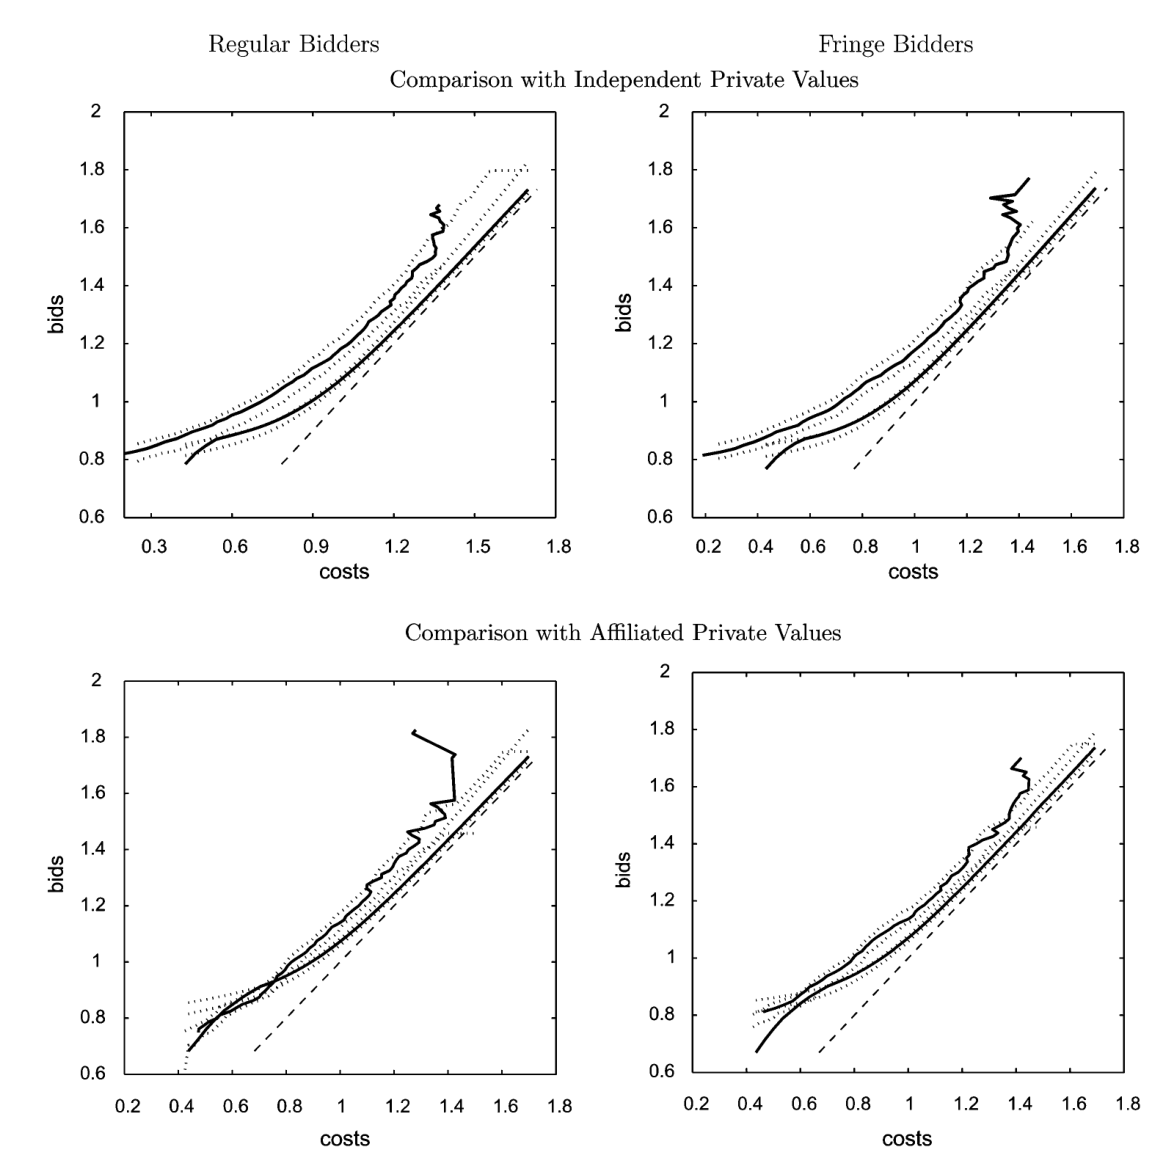
\includegraphics[width=0.86\textwidth]{figures/ch15/krasno_pub_fig5.png}
\caption{Expected bid functions, bids against costs in homogenized units, for regular (left) and
fringe (right) bidders. The top row compares the heterogeneity estimate with IPV, and the bottom row
compares it with APV. In each panel the dashed line is the diagonal. The lower solid line is the
estimate under unobserved heterogeneity, and the upper solid line is the misspecified estimate. Dotted
lines are pointwise 95 percent bootstrap bands. Source: Krasnokutskaya (2011), Figure 5.}
\label{fig:15-krasno-bidfn}
\end{figure}

\casehead{Reserve prices}
The estimates feed a design exercise (pp.~316--317). To avoid the complications of asymmetric
auctions, she uses the estimates for regular bidders only and treats bidders as symmetric. The
government minimizes the expected cost of procurement. If no bid falls below the maximum acceptable
price $r$, the project waits. Waiting costs $c_0$, which combines the cost of delay and the expected
cost of completing the work later. In the notation of \cref{sec:14-proc-other}, $c_0$ plays the role
of the buyer's value $u_0$. Suppose first that the government observes $\omega$. Costs then have the
distribution $F_C(c\mid\omega)=F_1\big(\frac{c}{\omega}\big)$ and density
$f_C(c\mid\omega)=\frac{1}{\omega}f_1\big(\frac{c}{\omega}\big)$. The virtual cost
\eqref{eq:14-virtual-cost} is
\[
J(c\mid\omega)=c+\frac{F_C(c\mid\omega)}{f_C(c\mid\omega)}
=c+\omega\,\frac{F_1(\frac{c}{\omega})}{f_1(\frac{c}{\omega})}
=\omega\,J_1\Big(\frac{c}{\omega}\Big),
\qquad J_1(a)=a+\frac{F_1(a)}{f_1(a)} .
\]
The optimal maximum price solves $J(r^*\mid\omega)=c_0$, so that
\[
r^*(\omega)=\omega\,J_1^{-1}\Big(\frac{c_0}{\omega}\Big).
\]
The reserve does not scale with $\omega$, because $c_0$ is fixed in dollars. This benchmark is case
(a) of her four candidates. In case (b) the government does not observe $\omega$. It chooses one reserve
that minimizes the expected cost averaged over $F_\omega$. Cases (c) and (d) use the cost distributions
estimated under IPV and APV. Each candidate is evaluated under the heterogeneity model. Since $c_0$ is
not observed, she reports results for several values.

\Cref{tab:15-krasno-reserve} reproduces her Table 4 for projects with an engineer's estimate of
\$400,000. Reserves based on IPV estimates raise the expected cost above the benchmark by 8.3 to 20.6
percent of $c_0$, which she rounds to 9 to 20 percent. Relative to the benchmark cost, the increase is 10
to 35 percent. The reserve of case (b) costs only
about 1 percent of $c_0$, or 1 to 2 percent of the benchmark. APV-based reserves do worse still. Both
misspecified models also imply too low a probability that any bid is submitted. For $c_0$ of at
least 150 percent of the mean cost, which she regards as the realistic range, accounting for
heterogeneity saves at least 16 percent of the benchmark cost (p.~317). This is large next to markups
of only 6 to 8 percent of costs.

\begin{table}[htbp]
\centering
\caption{Optimal reserve prices under alternative models (Krasnokutskaya 2011, Table 4)}
\label{tab:15-krasno-reserve}
{\small
\setlength{\tabcolsep}{4pt}
\begin{tabular}{clcccc}
\toprule
 & & \multicolumn{2}{c}{Unobserved heterogeneity} & & \\
\cmidrule(lr){3-4}
$c_0$ & & Benchmark (a) & Expected (b) & IPV (c) & APV (d)\\
\midrule
5 & Probability of a bid & 0.29 & 0.28 & 0.07 & 0.03\\
  & & (0.26, 0.31) & (0.25, 0.31) & (0.05, 0.09) & (0.02, 0.06)\\
  & Expected cost, \% of $c_0$ & 85.2 & 86.5 & 93.5 & 96.8\\
  & & (83, 87) & (85, 88) & (91, 95) & (95, 98)\\
  & Expected cost, \% of benchmark & & 101.4 & 109.7 & 113.6\\
\addlinespace
7 & Probability of a bid & 0.45 & 0.42 & 0.20 & 0.04\\
  & & (0.43, 0.46) & (0.40, 0.43) & (0.18, 0.21) & (0.03, 0.05)\\
  & Expected cost, \% of $c_0$ & 72.1 & 73.2 & 83.9 & 95.4\\
  & & (71.2, 73.5) & (72.3, 75.1) & (81.2, 84.7) & (94.3, 96.2)\\
  & Expected cost, \% of benchmark & & 101.6 & 116.4 & 132.4\\
\addlinespace
10 & Probability of a bid & 0.58 & 0.55 & 0.20 & 0.037\\
   & & (0.56, 0.59) & (0.54, 0.56) & (0.18, 0.21) & (0.03, 0.04)\\
   & Expected cost, \% of $c_0$ & 58.1 & 59.1 & 78.7 & 94.7\\
   & & (56.2, 59.5) & (57.8, 60.1) & (76.5, 79.7) & (94.0, 95.6)\\
   & Expected cost, \% of benchmark & & 101.6 & 135.5 & 163.0\\
\bottomrule
\end{tabular}}

\smallskip
\begin{minipage}{0.93\textwidth}
\footnotesize \textit{Notes.} Projects with an engineer's estimate of \$400,000, regular bidders treated as
symmetric. $c_0$ is the cost of not awarding the project today, in hundreds of thousands of dollars.
(a) The government observes $\omega$. (b) One reserve minimizes the cost averaged over $F_\omega$. (c),
(d) Reserves computed from IPV and APV estimates. All candidates are evaluated under the heterogeneity
estimates. Intervals in parentheses as printed.
\end{minipage}
\end{table}

\casehead{Tests of the assumptions and robustness}
Her Table 3 reports tests of the restrictions of Proposition 2 (pp.~317--318). The ratio test (W3)
of Section 5.2 gives a $p$-value of 0.52. Independence of the private components from $\omega$ gives
0.81 (bootstrap) and 0.75 (subsampling). Independence of the private components across bidders gives
0.43 and 0.63. The text adds a $p$-value of 0.63 for the test of part 1 of Proposition 2. None of the
tests rejects.
One robustness check addresses dynamics. Capacity constraints would link bids across auctions and bias
the estimated joint characteristic function. She re-estimates the model on projects for which every
regular bidder's backlog lies between 30 and 75 percent of the largest backlog observed in the data.
The sample shrinks and the estimates are less precise, but the variance decomposition and the biases
from misspecification are similar (pp.~318--319). The WP adds a fit check. Pseudo-bids simulated from
the estimated model reproduce the estimated densities of actual bids, with the largest gap near the
mode (WP, p.~28, Figure 3c).

\subsubsection{Assessment}

Krasnokutskaya's paper gave the first nonparametric identification result for first-price auctions
with unobserved heterogeneity. It turned the repeated-measurement idea into an auction estimator, and it
quantified how IPV and APV estimators err. In Michigan resurfacing, private information explains only
about a third of cost variation, 34 percent of the variation in total costs (p.~319). The remaining
two thirds is common knowledge among bidders. Ignoring it raises the estimated average markup of
regular bidders from 8.4 percent to 14 percent (APV) or 19 percent (IPV). Reserve prices based on the
misspecified models would raise procurement costs by 10 to 63 percent of the benchmark. The asymmetry
between regular and fringe firms matters less, with inefficient awards in 5 percent of auctions at a
cost of 2 percent. \citet[p.~103]{HortacsuPerrigne2021} summarize the published findings in the same
terms. The WP's figures differ, with a 28 percent inefficiency rate and a private share of 15 or 25
percent, and the published article replaces them.

The approach has four limits. First, heterogeneity must be scalar and enter by a known separable
form, and the two-dimensional extension needs four bids. Second, independence of $\omega$ and $\bm A$
and across bidders is essential. Her tests do not reject it (Table 3), but they have limited power,
and the model leaves no room for affiliation among the private components. Third, estimation is cell
by cell in $(n,n_1)$ and covariates, with slow rates, and the published estimates rest on 226 projects.
\citet[footnote 22]{AtheyLevinSeira2011} give this reason for not using the method on timber data.
``[O]ne would want to estimate the model separately for each vector of participants $(n_L,n_M)$ and we
simply don't have the data to do this.'' Fourth, the number of bidders is taken as exogenous. Entry
that responds to $\omega_t$ would violate (D1), and Krasnokutskaya leaves participation to separate
work.

\citet{KrasnokutskayaSeim2011} add participation in later work on California highway procurement,
where small firms receive a bid preference \citep[p.~123]{HortacsuPerrigne2021}. They estimate an
entry model of the \citet{LevinSmith1994} type with cost asymmetries. Entry costs are 2.2 to 3.9
percent of the engineer's estimate for small firms and 3.1 to 3.3 percent for large firms. The state
aims to award 25 percent of procurement dollars to small firms. The authors first evaluate this goal for
one illustrative project \citep[pp.~2655--2656, Figure~1]{KrasnokutskayaSeim2011}. With fixed
participation, reaching the goal on that project requires a small-firm discount of more than 50 percent,
at a predicted cost increase of 0.23 percent. Allowing entry to respond, that discount would deter large
firms and raise the cost by 7.8 percent. A discount of about 20 percent then reaches the goal on the same
project, and the procurement cost rises by 3.2 percent. These figures describe a single project. For all
projects together, the article's text reports that a 15 percent discount approximately meets the aggregate goal, at a
cost increase of 1.4 percent (p.~2678). Their Table~11 instead lists, for the same 15 percent discount, a
small-firm share of work of 31.9 percent and a cost increase of 2.1 percent (p.~2679). The article does
not reconcile the two sets of numbers. \Cref{sec:14-proc-other} discusses the theory of such preferences. Later work relaxes separability.
\citet{HuMcAdamsShum2013} identify nonseparable heterogeneity from three bids per auction (as described
by \citealp{Roberts2013}, p.~5). \citet{Asker2010} applies the deconvolution to knockout bids in a
stamp cartel (\cref{sec:13-asker-structural}).

\subsection{Parametric approaches}\label{sec:15-uh-param}

A parametric first step trades flexibility in the distributions for flexibility in how covariates
and heterogeneity enter. \citet{AtheyLevinSeira2011} specify Weibull bid distributions conditional on a
Gamma-distributed multiplicative component, which integrates out in closed form
(\cref{sec:15-als}, \cref{prop:15-als-lik}). Values then follow from the first-order condition at any
$\omega$, as in \cref{thm:15-krasno}. The parametric form lets heterogeneity affect types
differently and keeps estimation feasible with many participant configurations
\citep[Section 6.1.2]{AtheyHaile2007}. \citet{RobertsSweeting2013} estimate values with heterogeneity
in values and entry costs by simulated maximum likelihood with importance sampling (as described by
\citealp{Roberts2013}, p.~6). \citet{HongShum2002} model the median of the bid distribution as a normal
random variable whose mean depends on the number of bidders (as described by
\citealp{Krasnokutskaya2011}, p.~296). Finite mixtures of parametric distributions offer a middle
ground \citep[eqs. (6.7)--(6.9)]{AtheyHaile2007}. In all of these, identification of the
heterogeneity distribution leans on functional form.

\subsection{Reserve prices as a control for quality: Roberts (2013)}\label{sec:15-roberts}

\casehead{Idea}
Every method so far uses only bidders' behavior. \citet{Roberts2013} uses the seller's behavior. A
seller who knows the object well probably observes what the bidders observe. If the reserve price
rises with the unobserved quality, then reserve prices reveal it. The logic is that of a control
function, close to the use of investment as a proxy for productivity by \citet{OlleyPakes1996}.
\citet{Roberts2013} credits the suggestion to Athey and Haile, and \citet[footnote 56]{AtheyHaile2007}
point to restrictions from the seller's side as a direction worth exploring. His motivating evidence
is old. In the eggplant data of \citet{LaffontOssardVuong1995}, winning bids and reserve prices move
in tandem across auctions (\citealp{Roberts2013}, p.~7, citing their Appendix figure, reproduced in
\cref{fig:15-lov-reserve}).

\casehead{Model}
In auction $t$ there are $N_t$ bidders with symmetric independent private values. Observed
characteristics $Z_t$ and the scalar $\omega_t$ are known to the seller and the bidders, and the
econometrician observes only $Z_t$. Values are drawn from $F_V(\cdot\mid Z_t,\omega_t)$, which may depend
on $\omega_t$ in any way, but not on $N_t$. The seller sets the reserve price $r_t=m(Z_t,\omega_t)$ with
the same function $m$ in every auction. The bidders counted in $N_t$ include those with values below
$r_t$.

\begin{assumption}[\citealp{Roberts2013}, Assumption S1]\label{ass:15-roberts}
For every $z$, $m(z,\omega)$ is strictly increasing in $\omega$.
\end{assumption}

Reserves need not be optimal. Monotonicity is nevertheless what optimal reserves deliver when higher
$\omega$ makes higher values strictly more likely. Recall the virtual valuation \eqref{eq:14-psi} and write it conditionally on $\omega$ as
$\psi(t\mid\omega)=t-\frac{1-F_V(t\mid\omega)}{f_V(t\mid\omega)}$. The optimal reserve solves
$\psi(r^*\mid\omega)=v_0$, where $v_0$ is the seller's value (\cref{cor:14-optimal-reserve}).

\begin{proposition}[\citealp{Roberts2013}, Proposition 1]\label{prop:15-roberts1}
Suppose $\psi(t\mid\omega)$ is strictly increasing in $t$ for every $\omega$. If $V$ and $\omega$ are
affiliated, the optimal reserve price is nondecreasing in $\omega$. If they are strictly affiliated, so that the
likelihood ratio inequality below is strict for all $v_1<v_2$ and $\omega_1<\omega_2$, the optimal reserve price
is strictly increasing in $\omega$.
\end{proposition}

\begin{proof}
Take $\omega_1<\omega_2$. By \cref{prop:14-affil-mlrp}, affiliation gives the monotone likelihood ratio
property. For $v_1<v_2$,
$\frac{f_V(v_2\mid\omega_1)}{f_V(v_1\mid\omega_1)}\le\frac{f_V(v_2\mid\omega_2)}{f_V(v_1\mid\omega_2)}$,
strictly under strict affiliation. Integrating over $v_2>v_1$ gives
$\frac{1-F_V(v_1\mid\omega_1)}{f_V(v_1\mid\omega_1)}\le\frac{1-F_V(v_1\mid\omega_2)}{f_V(v_1\mid\omega_2)}$,
so the inverse hazard is nondecreasing in $\omega$ and $\psi(t\mid\omega_2)\le\psi(t\mid\omega_1)$ for every $t$.
Integration preserves strict inequality, so both inequalities are strict under strict affiliation. Let $r_1$
solve $\psi(r_1\mid\omega_1)=v_0$. Then $\psi(r_1\mid\omega_2)\le v_0$. Since $\psi(\cdot\mid\omega_2)$ is
strictly increasing, the solution $r_2$ of $\psi(r_2\mid\omega_2)=v_0$ satisfies $r_2\ge r_1$. Under strict
affiliation $\psi(r_1\mid\omega_2)<v_0$, and therefore $r_2>r_1$.
\end{proof}

Affiliation alone does not deliver \cref{ass:15-roberts}. Independent $V$ and $\omega$ are affiliated, yet the
optimal reserve then does not move with $\omega$. With $V$ uniform on $[0,1]$ and $v_0=0$, for example,
$r^*=\frac12$ for every $\omega$. The proof in \citet[Appendix~B]{Roberts2013} writes the affiliation inequality
as strict, which is the strict case of the proposition.

The second result is the identification theorem. Partition $Z=(Z_0,Z_1)$.

\begin{proposition}[\citealp{Roberts2013}, Proposition 2]\label{prop:15-roberts2}
Let \cref{ass:15-roberts} hold. Suppose (i) there is a value $z_1^*$ such that $m(z_0,z_1^*,\omega)=\omega$
for all $z_0$ and $\omega$, and (ii) $\omega$ is independent of $Z_1$ conditional on $Z_0$. Then reserve prices
identify $F_{\omega\mid Z_0}$, the function $m$ and each realization $\omega_t$. Suppose in addition that the
number $N$ of potential bidders is known and that unsold auctions are recorded. Then transaction prices identify
$F_V(v\mid Z,\omega)$ for every $v\ge m(Z,\omega)$, including the mass $F_V\big(m(Z,\omega)\mid Z,\omega\big)$, in
first-price and second-price (or ascending) auctions.
\end{proposition}

\begin{proof}
\emph{Step 1 (the law of $\omega$).} By (i) and (ii),
\[
\Pr(r_t\le u\mid Z_0=z_0,Z_1=z_1^*)=\Pr(\omega_t\le u\mid Z_0=z_0,Z_1=z_1^*)=F_{\omega\mid Z_0}(u\mid z_0).
\]
\emph{Step 2 (the function $m$).} For any $z_1$, monotonicity and (ii) give
\[
F_{\omega\mid Z_0}(u\mid z_0)=\Pr\big(m(z_0,z_1,\omega_t)\le m(z_0,z_1,u)\mid z_0,z_1\big)=F_{r\mid Z}\big(m(z_0,z_1,u)\mid z_0,z_1\big),
\]
so $m(z_0,z_1,u)=F_{r\mid Z}^{-1}\big(F_{r\mid Z}(u\mid z_0,z_1^*)\mid z_0,z_1\big)$ is identified.
\emph{Step 3 (realizations).} Since $m$ is strictly increasing in $\omega$, each observed $(r_t,Z_t)$
reveals $\omega_t=m^{-1}(Z_t,r_t)$.
\emph{Step 4 (values).} Treat $(Z_t,\omega_t)$ as observed covariates. For fixed $(Z,\omega)$ the
reserve $m=m(Z,\omega)$ is fixed, so transaction prices are censored at it. For $v\ge m$ let $W(v)$ be the
probability that the object goes unsold or sells at a price of at most $v$. Unsold auctions enter $W$, which
is why they must be recorded. In a second-price or ascending auction, the second-highest of the $N$ values is
at most $v$ exactly when this event occurs, so $W(v)=\Lambda_{N-1:N}\big(F_V(v\mid Z,\omega)\big)$. Inverting
$\Lambda_{N-1:N}$, which requires $N$, gives $F_V(v\mid Z,\omega)$. In a first-price auction whose bidders know $N$
but not who participates, as in \cref{sec:15-gpv-reserve}, let $\xi$ be the inverse bid function above the
reserve. The event occurs at a bid level $b\ge m$ when every potential bidder
stays out or bids at most $b$, so $W(b)=F_V\big(\xi(b)\mid Z,\omega\big)^N$. A bidder's win probability is
$W(b)^{\frac{N-1}{N}}$, and the first-order condition gives $\xi(b)=b+\frac{N}{N-1}\frac{W(b)}{W'(b)}$, as in
\eqref{eq:15-winbid-xi}. Then $F_V\big(\xi(b)\mid Z,\omega\big)=W(b)^{\frac1N}$. In both formats $W(m)$, the
probability of no sale or a sale at the reserve, gives the mass at $m$.
\end{proof}

With less data the conclusion narrows. Without $N$ the transformation from $W$ to $F_V$ is unknown, and without
the unsold auctions the prices of sold objects do not determine $W$. In second-price and ascending auctions that
record the number of actual bidders, transaction prices still identify the value distribution truncated at the
reserve, by \cref{prop:15-reserve-ident}(i).

\Citet[Proposition 2]{Roberts2013} states the result without the restriction $v\ge m(Z,\omega)$ and
without the requirements on $N$ and on unsold auctions. His proof cites \citet[Theorems 1 and 6]{AtheyHaile2002},
which assume no binding reserve. Below the
reserve, no bid is recorded and the data carry no information about $F_V(\cdot\mid Z,\omega)$, as in
\cref{thm:15-gpv-reserve}. The reserve does bind in his data, since 107 of 1,117 cars in one subsample
go unsold.

The normalization (i) holds in many functional forms, for example $r=z\,\omega$ or $r=z+\omega$ at a
suitable $z$ (\citealp{Roberts2013}, footnote 6). Unlike \cref{thm:15-krasno}, the result allows values
to depend on $\omega$ in any way. Among bids it needs only the transaction price, together with $N$ and the
record of unsold auctions. It requires instead that the
reserve depend on nothing that the bids do not reflect.

\casehead{Setting and data}
The data come from a wholesale used-car auction house in Suwon, South Korea, which held weekly auctions
between October 10, 2001 and November 27, 2002 (\citealp{Roberts2013}, Section 3).
Only registered dealers may bid, and more than 380 were registered. The house charges the seller \$50
per car and collects 2.2 percent of the price from each side if the car sells. Sellers set reserve
prices, usually with guidance from the house. Dealers receive car descriptions three days ahead and
inspect the cars for three hours or more before the auction. The format is a button auction with
reentry. The price rises by \$30 every three seconds while at least two buttons are pressed, and bidders
cannot see when rivals drop out. Of 28,334 passenger cars, Roberts studies 4,943 automatic
five-passenger sedans. Hyundai, Daewoo and Kia account for 42, 39 and 18 percent of auctions. The
average winning bid is \$3,661.83, the average reserve \$3,361.26, and 5.37 bidders bid on the
average car (\citealp{Roberts2013}, Table 1). Among bids, only the transaction price is recorded,
together with the identities of the winner and the runner-up and the number of bidders.

\casehead{Evidence for the assumptions}
Several facts support the model (\citealp{Roberts2013}, pp.~13--19). In regressions of the log
winning bid on car characteristics and dummies, $R^2$ rises from $0.903$ to $0.979$ when the log
reserve is added. The log reserve alone gives $0.966$ (Table 2). The residuals of winning bids and of
reserves, after both are regressed on characteristics, have correlation $0.890$, against a raw
correlation of $0.983$. For 107 unsold cars among 1,117 auctioned between October 10 and December 27,
2001, the same residual correlations are $0.942$ for the highest bid and $0.943$ for the average bid.
The reserve does not predict failure to sell. Its coefficient in a logit is $0.232$ with standard error
$0.263$ (Table 4). Moving the reserve from its 25th to its 75th percentile raises the failure
probability by about 2 percentage points. Reserves do not rise with the number of bidders, which a
signaling model of reserves would predict \citep{CaiRileyYe2007}. About four of the roughly five
bidders per car bid above the reserve, so the co-movement is not mechanical. Bidders look symmetric.
Three quarters of them buy 17 or fewer cars over 59 auction days.

\casehead{Estimation}
For Hyundai Sonatas, Roberts specifies $m(Z_1,\omega)=\mu(X;\vartheta)+\omega$ with $\E[\omega X]=0$
(p.~19). Here $X$ collects age and mileage. The function $\mu$ is quadratic in them, including their
interaction. The residual of this regression estimates $\omega_t$. The distribution of transaction prices $P_t$ given
$Z=(Z_1,\hat\omega)$ is estimated by a kernel estimator of a conditional distribution (his eq. (3)),
\[
\hat F_{P\mid Z=z}(v)=\frac{\sum_{t=1}^T\tilde{\mathcal K}_1\big(\frac{v-P_t}{h}\big)\,\mathcal K_2\big(\frac{z-Z_t}{h}\big)}{\sum_{t=1}^T\mathcal K_2\big(\frac{z-Z_t}{h}\big)},
\]
where $\tilde{\mathcal K}_1$ is the integral of a kernel $\mathcal K_1$. Gaussian kernels and Silverman's
bandwidth are used. Bid increments are ignored, so the transaction price is the second-highest of $N$
values, and $\hat F_V(v\mid z)=\Lambda_{N-1:N}^{-1}\big(\hat F_{P\mid Z=z}(v)\big)$ (his eq. (2), our
\eqref{eq:15-Lambda}). By \cref{prop:15-roberts2}, this inversion is valid for $v$ at or above the
reserve, and only if unsold auctions enter $\hat F_{P\mid Z}$ as described in Step 4. Roberts does not
treat the reserve as a censoring point. Since about four of the roughly five bidders per car bid above
the reserve, the censoring mainly affects the lower tail of the estimated value distribution.
Consistency with a generated regressor follows from conditions in \citet{Matzkin2003}. Roberts pools months with similar numbers of unique bidders, whose average is
$62.6$. He drops auctions with more than eight bidders, which keeps over 92 percent of them, and sets
$N=8$. The restricted sample has 454 Sonatas, with mean winning bid \$3,574.38, mean reserve
\$3,320.22, mean age $84.10$ months and $4.83$ unique bids per car (Table 5). In this sample the
adjusted $R^2$ of the log winning bid rises from $0.773$ to $0.971$ with the reserve, and the residual
correlation is $0.9343$ against a raw $0.9835$.

\casehead{Results}
\Cref{fig:15-roberts-cdf} shows estimated value distributions for a seven-year-old Sonata with 100,000
km. Ignoring heterogeneity produces a much more dispersed distribution. Controlling for it, the
distributions at the 10th, 50th and 90th percentiles of $\omega$ are ordered by first-order stochastic
dominance. Their means are \$1,919.61, \$2,426.20 and \$2,971.17, with bootstrap 95 percent intervals
$[1{,}904.37,1{,}937.11]$, $[2{,}406.88,2{,}448.65]$ and $[2{,}946.99,2{,}999.08]$ (p.~22). With $N=7$ the
means are \$2,168.82, \$2,542.19 and \$3,146.35, and with $N=9$ they are \$1,871.81, \$2,326.22 and
\$2,788.02 (footnote 9). A parametric alternative with lognormal values and a Poisson number of bidders
gives \$1,758.45, \$2,184.41 and \$2,864.57, with an estimated mean of $8.84$ bidders (footnote 10).

\begin{figure}[htbp]
\centering
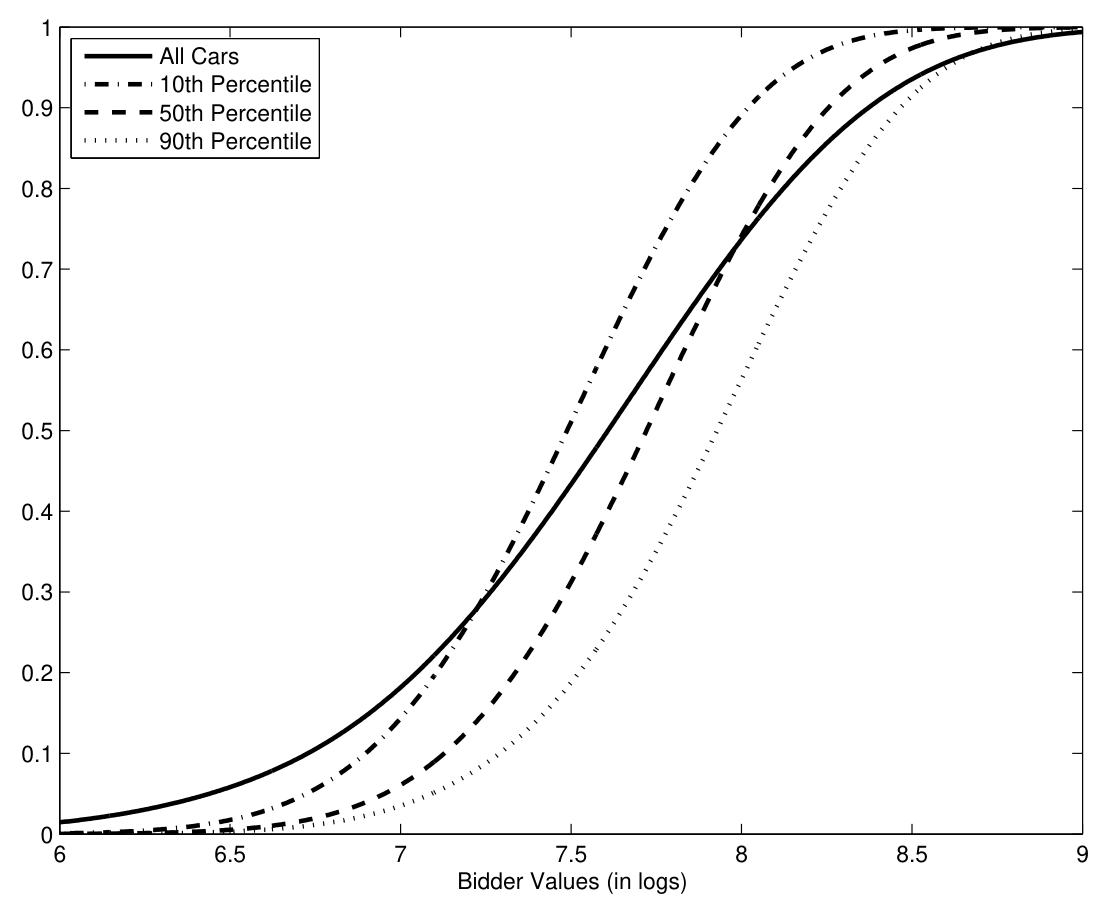
\includegraphics[width=0.62\textwidth]{figures/ch15/roberts_fig1.png}
\caption{Estimated value distributions (log values) for seven-year-old automatic Hyundai Sonatas with
100,000 km. Solid line: ignoring unobserved heterogeneity. Other lines: controlling for it at the 10th,
50th and 90th percentiles of $\omega$. Source: Roberts (2013), Figure 1 (June 2013 working-paper version).}
\label{fig:15-roberts-cdf}
\end{figure}

\casehead{Counterfactuals}
Roberts asks how much of the attainable value sellers capture and through which channels. He sets the
seller's value to $v_0=\gamma r$ for $\gamma\in\{0,0.25,0.5,0.75\}$ and simulates revenues with
$N=8$. \Cref{tab:15-roberts-reserve} reproduces his Table 6. Ignoring heterogeneity overstates the
dispersion of values and pushes the estimated optimal reserve up. A sufficient condition is hazard rate
dominance. Let $\lambda_C$ and $\lambda_{NC}$ be the hazard rates of the value distributions estimated
with and without the control, and suppose $\lambda_C(r)>\lambda_{NC}(r)$ for all $r$. The optimal
reserve with the control solves $r_C=v_0+\frac{1}{\lambda_C(r_C)}<v_0+\frac{1}{\lambda_{NC}(r_C)}$, so
$\psi_{NC}(r_C)<v_0$. Regularity then gives $r_{NC}>r_C$ (\citealp{Roberts2013}, footnote 13). With
actual reserves, the mean seller captures between 88.42 and 92.23 percent of the value of the optimal
auction with the same bidders, depending on $\gamma$. Using the ``optimal'' reserves computed while
ignoring heterogeneity would lower the mean share to between 85.53 and 88.93 percent. The text
summarizes the first result as ``around 94\%'' (p.~25), above every mean and median in the table. The
figure is close to the 90th-percentile column, 93.08 to 94.51 percent. The text also says that 90
percent of sellers achieve more than 83 percent, which matches the 10th percentile of 83.69 at
$\gamma=0$.

\begin{table}[htbp]
\centering
\caption{Optimal reserve prices and the share of value captured by sellers (Roberts 2013, Table 6)}
\label{tab:15-roberts-reserve}
{\small
\setlength{\tabcolsep}{4pt}
\begin{tabular}{ccccccccccc}
\toprule
 & \multicolumn{2}{c}{Difference in optimal reserve} & \multicolumn{4}{c}{Actual reserves (\%)} & \multicolumn{4}{c}{Reserves ignoring UH (\%)}\\
\cmidrule(lr){2-3}\cmidrule(lr){4-7}\cmidrule(lr){8-11}
$\gamma$ & Overall & Median & Mean & 10th & 50th & 90th & Mean & 10th & 50th & 90th\\
\midrule
0.00 & \$221.57 & \$77.21 & 88.42 & 83.69 & 89.18 & 93.08 & 85.53 & 77.37 & 94.08 & 94.70\\
     & (25.36) & (24.89) & (0.19) & (0.33) & (0.18) & (0.14) & (0.13) & (0.17) & (0.03) & (0.04)\\
0.25 & 258.52 & 90.20 & 90.66 & 86.69 & 91.69 & 93.53 & 86.58 & 74.62 & 94.10 & 94.70\\
     & (23.16) & (25.52) & (0.18) & (0.38) & (0.13) & (0.05) & (0.11) & (0.13) & (0.03) & (0.03)\\
0.50 & 239.72 & 98.45 & 92.23 & 86.98 & 93.69 & 94.25 & 87.60 & 74.05 & 94.05 & 94.70\\
     & (21.35) & (21.01) & (0.20) & (0.64) & (0.04) & (0.03) & (0.08) & (0.11) & (0.03) & (0.02)\\
0.75 & 236.03 & 123.57 & 91.81 & 85.84 & 93.45 & 94.51 & 88.93 & 80.42 & 94.04 & 94.71\\
     & (21.79) & (22.12) & (0.20) & (0.76) & (0.07) & (0.04) & (0.07) & (0.08) & (0.03) & (0.02)\\
\bottomrule
\end{tabular}}

\smallskip
\begin{minipage}{0.93\textwidth}
\footnotesize \textit{Notes.} $v_0=\gamma r$, with $r$ the observed reserve. ``Overall'' is the average
difference across all cars, and ``Median'' the average for cars with $\omega$ within half a standard
deviation of its median. The paper's column header, and its definition on p.~24, write the difference
as $R^*_C-R^*_{NC}$. The table note describes it as the optimal reserve ignoring heterogeneity minus
the optimal reserve controlling for it. The text and its footnote 13 say that ignoring heterogeneity
raises the optimal reserve. The positive entries agree with the note, which we follow. The remaining columns give the percentage of the value of the
optimal auction captured with actual reserves and with the ``optimal'' reserves that ignore
heterogeneity. Bootstrap standard errors (100 repetitions) in parentheses, in percentage points for
percentages.
\end{minipage}
\end{table}

\Cref{tab:15-roberts-channels} reproduces Table 7, which decomposes the value of the platform with
$\gamma=0$. Let $\pi^N_{r}$ denote revenue with $N$ bidders and reserve $r$. The first row is the gain
$\pi^{N+1}_{r=r^*}-\pi^N_{r=0}$ from one more bidder together with an optimal reserve. The next rows split
the gain into the extra bidder, $\pi^{N+1}_{r=0}-\pi^N_{r=0}$, and the reserve,
$\pi^{N+1}_{r=r^*}-\pi^{N+1}_{r=0}$. The extra bidder dominates, as the theorem of
\citet{BulowKlemperer1996} suggests (\cref{prop:14-bk}). With four bidders, the extra bidder is
worth $\frac{94.49}{5.51}\approx17.1$ times as much as the optimal reserve when heterogeneity is
controlled for, and $\frac{81.89}{18.11}\approx4.5$ times as much when it is not. With five bidders the ratios are $26.1$ and $5.1$.
The text reports 17.5 and 4.6 ``when there are five bidders'' (p.~26), close to our ratios for $N=4$, where
the extra bidder makes five.
Ignoring heterogeneity overstates the role of reserves and understates the role of competition.

\begin{table}[htbp]
\centering
\caption{Channels through which sellers gain from the auction house (Roberts 2013, Table 7)}
\label{tab:15-roberts-channels}
\begin{tabular}{lcccccc}
\toprule
$N$ & 2 & 3 & 4 & 5 & 6 & 7\\
\midrule
\multicolumn{7}{l}{\emph{Controlling for unobserved heterogeneity}}\\
Gain $\pi^{N+1}_{r=r^*}-\pi^{N}_{r=0}$ (\$) & 725.94 & 435.5 & 307.89 & 233.09 & 189.07 & 160.59\\
 & (14.95) & (8.98) & (6.56) & (5.13) & (4.23) & (3.49)\\
Share from extra bidder (\%) & 87.71 & 91.91 & 94.49 & 96.31 & 97.31 & 97.97\\
 & (0.41) & (0.39) & (0.34) & (0.31) & (0.31) & (0.34)\\
Share from optimal reserve (\%) & 12.29 & 8.09 & 5.51 & 3.69 & 2.69 & 2.03\\
 & (0.41) & (0.39) & (0.33) & (0.30) & (0.31) & (0.34)\\
\addlinespace
\multicolumn{7}{l}{\emph{Not controlling for unobserved heterogeneity}}\\
Gain $\pi^{N+1}_{r=r^*}-\pi^{N}_{r=0}$ (\$) & 871.61 & 578.62 & 426.34 & 333.26 & 276.46 & 229.27\\
 & (13.02) & (7.97) & (6.38) & (5.33) & (4.74) & (4.03)\\
Share from extra bidder (\%) & 75.38 & 79.11 & 81.89 & 83.68 & 85.43 & 86.46\\
 & (0.92) & (1.06) & (1.15) & (1.26) & (1.28) & (1.35)\\
Share from optimal reserve (\%) & 24.62 & 20.89 & 18.11 & 16.32 & 14.57 & 13.54\\
 & (0.92) & (1.07) & (1.15) & (1.25) & (1.28) & (1.36)\\
\bottomrule
\end{tabular}

\smallskip
\begin{minipage}{0.93\textwidth}
\footnotesize \textit{Notes.} $\gamma=0$. Shares are
$\frac{\pi^{N+1}_{r=0}-\pi^N_{r=0}}{\pi^{N+1}_{r=r^*}-\pi^N_{r=0}}$ and
$\frac{\pi^{N+1}_{r=r^*}-\pi^{N+1}_{r=0}}{\pi^{N+1}_{r=r^*}-\pi^N_{r=0}}$. Revenues from 10,000 simulations.
Bootstrap standard errors (100 repetitions) in parentheses, in percentage points for percentages.
\end{minipage}
\end{table}

\casehead{Assessment}
Roberts showed that seller behavior can carry information about what the econometrician misses. The
method needs only transaction and reserve prices and a record of unsold auctions. It lets values depend
on $\omega$ without separability. Its requirements are strong in other directions. Heterogeneity must be scalar and enter
both the reserve and the bids. The seller may have no private information that bidders value, and the
reserve may respond to nothing that bidders ignore. All sellers must use one reserve rule, which the
auction house's guidance makes plausible. Bidders must be symmetric, and the number of potential
bidders must be assumed. The estimates of the reserve function are parametric. Within these limits,
the paper adds the seller as a second source of information about unobserved quality, and it measures
the Bulow-Klemperer comparison in a real market.

\subsection{Comparing the approaches}\label{sec:15-uh-compare}

\Cref{tab:15-uh-approaches} summarizes the approaches. They differ in the data they demand and in the
restrictions they place on how heterogeneity enters. The number of bidders can itself serve as a control
when it is a sufficient statistic for the heterogeneity \citep[Section 3.2]{CampoPerrigneVuong2003}. It
can also serve as an instrument when participation depends on an excluded variable
\citep{HaileHongShum2003}, as discussed in \cref{sec:15-cv}.

\begin{table}[htbp]
\centering
\caption{Approaches to unobserved auction heterogeneity}
\label{tab:15-uh-approaches}
{\footnotesize
\begin{tabularx}{\textwidth}{>{\raggedright\arraybackslash}p{2.35cm}>{\raggedright\arraybackslash}X>{\raggedright\arraybackslash}X>{\raggedright\arraybackslash}X>{\raggedright\arraybackslash}p{2.3cm}}
\toprule
Approach & Data required & Restrictions & What is identified & Practical cost\\
\midrule
Homogenization (\cref{sec:15-uh-sep}) & Bids and observed covariates & All heterogeneity observed. Separable covariate effect & $F_V(\cdot\mid z)$ and the covariate effect $g_0$ & Low\\
Deconvolution \citep{Krasnokutskaya2011} & At least two bids per auction, bidder types & Scalar $\omega$, separable. Components $\omega$ and $A_i$ mutually independent & $F_\omega$ and each $F_k$, not realizations & High: cell by cell, slow rates\\
Parametric mixture \citep{AtheyLevinSeira2011} & All bids & Parametric bid laws. Heterogeneity $\omega$ independent of covariates & Parameters, then $F_k(\cdot\mid\omega)$ for any $\omega$ & Moderate\\
Reserve-price control \citep{Roberts2013} & Transaction and reserve prices, record of unsold auctions & Reserve strictly increasing in scalar $\omega$. No seller private information & $m$, $F_\omega$, realizations of $\omega$, $F_V(\cdot\mid z,\omega)$ above the reserve & Moderate. $N$ assumed\\
$n$ as control or instrument \citep{CampoPerrigneVuong2003,HaileHongShum2003} & Bids, $n$, excluded shifters of participation & $n$ sufficient for $\omega$, or monotone in it & Value distributions given the control & Moderate\\
Three bids \citep{HuMcAdamsShum2013} & At least three bids per auction & Heterogeneity may enter values nonseparably & Model primitives with nonseparable heterogeneity & High\\
\bottomrule
\end{tabularx}}
\end{table}

\section{Entry, Participation, Dynamics and Risk Aversion}\label{sec:15-entry}

The identification results so far treat the set of bidders as given, each auction as a separate game,
and bidders as risk neutral. This section relaxes each assumption in turn. The theory of entry is in
\cref{sec:14-entry}, and the timber application, where entry costs are estimated, is in
\cref{sec:15-als}.

\subsection{Potential and actual bidders}\label{sec:15-entry-sets}

Following \citet[Section 6.3]{AtheyHaile2007}, let $\mathcal N$, with $|\mathcal N|=N$, be the set of
potential bidders, those who draw signals and decide whether to bid. Let
$\mathcal A\subseteq\mathcal N$, with $|\mathcal A|=n$, be the set of actual bidders, those who
place a bid. These are the objects of \cref{sec:15-gpv-reserve}, now written as sets. Both sets can vary across auctions. The set of potential bidders varies when acquiring a
signal is costly. The set of actual bidders varies, for a given $\mathcal N$, when a reserve price
binds or bidding is costly. The consequences for equilibrium and for identification depend on two
questions. Do bidders know who participates? Does the econometrician observe $\mathcal N$, $\mathcal A$,
or only $n$?

\subsection{Selection by a reserve price or a bid cost}\label{sec:15-entry-reserve}

A binding reserve price selects bidders with values above $r$. In ascending auctions with independent
private values, participants' values are draws from the truncated distribution, and observing
$\mathcal N$ restores $F_V$ above $r$ (\cref{prop:15-reserve-ident}). In first-price auctions, the inversion
with a reserve and an unknown number of potential bidders is \eqref{eq:15-gpv-reserve}
(\cref{thm:15-gpv-reserve}). \citet[Section 6.3.1]{AtheyHaile2007} extend the first-price results to
private values with correlation. Suppose bidders do not know $\mathcal A$ when they bid, which is natural
because participation depends on private information. The distribution of the highest rival bid then
mixes over the possible participant sets,
\[
G_{M_i\mid B_i}(m\mid b;\mathcal N)=\Pr\big(\mathcal A=\{i\}\mid i\in\mathcal A,B_i=b\big)+\sum_{\mathcal A'\ni i,\,|\mathcal A'|>1}
\Pr\Big(\mathcal A=\mathcal A',\ \max_{k\in\mathcal A',k\neq i}B_k\le m\ \Big|\ B_i=b\Big).
\]
Each piece is observable, so the first-order condition \eqref{eq:14-apv-foc} still maps each bid to a
value. Two results follow \citep[Theorems 6.4--6.5]{AtheyHaile2007}. First, for each $\mathcal A$, the
joint distribution of values of participants above $r$ is identified from $r$, all bids and bidder
identities. Second, each marginal $F_{V_i}(v)$ is identified for $v\ge r$, since
$F_{V_i}(r)=\Pr(i\notin\mathcal A)$ is observed when $\mathcal N$ is. Nothing can be learned about
correlation among values below $r$. A cost of preparing a bid acts like a reserve price, since only
bidders with high enough values bid \citep[footnote 60, citing \citealp{Samuelson1985} and
\citealp{HaileHongShum2003}]{AtheyHaile2007}.

\subsection{Costly signal acquisition and the entry cost}\label{sec:15-entry-cost}

In the model of \citet{LevinSmith1994}, firms pay $K$ to learn their values and then bid
(\cref{sec:14-entry}). In the symmetric equilibrium firms randomize, so the set of entrants
$\tilde{\mathcal N}$ varies exogenously. Entrants learn who else entered before bidding. If the reserve
price lies below every value, it binds only when a single firm enters, and that firm bids the reserve.
The randomization is useful twice. It creates exogenous variation in the number of bidders, which the
tests of \cref{sec:15-cv} require. It also identifies the entry cost.

\begin{proposition}[Entry costs, \citealp{AtheyHaile2007}, Section 6.3.2]\label{prop:15-entry-ident}
Suppose entry generates exogenous variation in $\tilde{\mathcal N}$ and the reserve lies below the
support of values. Suppose the econometrician observes the entrants and all their bids. Under IPV the
winning bid suffices.
\begin{enumerate}[label=(\roman*)]
\item Each entrant's expected gross profit $\pi_i(\mathcal A)$ in \eqref{eq:14-entry-profit-id} is
identified for every participant set $\mathcal A$ with $|\mathcal A|\ge2$ that occurs with positive
probability.
\item For any firm that randomizes, the entry cost is identified by \eqref{eq:14-entry-cost-id},
$K=\sum_{\mathcal A\ni i}\Pr\big(\tilde{\mathcal N}=\mathcal A\mid i\in\tilde{\mathcal N}\big)\,\pi_i(\mathcal A)$.
\end{enumerate}
In the symmetric IPV first-price auction with $n$ entrants,
\begin{equation}\label{eq:15-entry-profit}
\pi(n)=\E_B\Big[\frac{G_n(B)^n}{(n-1)\,g_n(B)}\Big],\qquad
\hat\pi(n)=\frac{1}{nT_n}\sum_{t:\,n_t=n}\ \sum_{i=1}^{n}\frac{\hat G_n(b_{it})^n}{(n-1)\,\hat g_n(b_{it})},
\end{equation}
where $G_n$ and $g_n$ are the bid distribution and density in $n$-bidder auctions.
\end{proposition}

\begin{proof}
(i) Exogenous variation in $\tilde{\mathcal N}$ means that bids in auctions with participant set
$\mathcal A$ are equilibrium bids for that set. The first-order condition identifies the value behind
each bid (\cref{sec:15-gpv,sec:15-apv}). Then $\pi_i(\mathcal A)$ is the expectation, over $i$'s bids, of
the margin times the probability of winning, both functions of observables. (ii) A firm that
randomizes is indifferent, so its expected gross profit from entry equals $K$. The probabilities of
each participant set are observed. For the formula, a bidder who bids $b$ against $n-1$ symmetric
rivals wins with probability $G_n(b)^{n-1}$ and has margin
$\xi(b)-b=\frac{G_n(b)}{(n-1)g_n(b)}$ by \eqref{eq:15-gpv-xi}. Its expected profit is
\[
\big(\xi(b)-b\big)G_n(b)^{n-1}=\frac{G_n(b)}{(n-1)g_n(b)}\,G_n(b)^{n-1}=\frac{G_n(b)^n}{(n-1)g_n(b)} .
\]
Averaging over the bid distribution gives \eqref{eq:15-entry-profit}. The sample analogue replaces $G_n$
and $g_n$ by the GPV estimates.
\end{proof}

\begin{example}[Recovering the entry cost]\label{ex:15-entry-uniform}
Take uniform values on $[0,1]$ and no reserve. In $n$-bidder auctions bids are uniform on
$[0,c]$ with $c=\frac{n-1}{n}$, so $G_n(b)=\frac{b}{c}$ and $g_n=\frac{1}{c}$. Then
\[
\pi(n)=\int_0^c\Big(\frac{b}{c}\Big)^n\frac{c}{n-1}\,\frac{db}{c}=\frac{c}{n-1}\int_0^1u^n\,du=\frac{c}{(n-1)(n+1)}=\frac{1}{n(n+1)},
\]
which matches \cref{lem:14-pi-decreasing}. A lone entrant pays the reserve and earns
$\pi(1)=\E[V]=\frac{1}{2}$, where $\E[V]$ is identified from bids in auctions with two or more entrants.
Suppose there are $N=5$ potential entrants and the observed entry probability is $0.816$. The number of
rival entrants is binomial, so
$K=\sum_{n=1}^5\binom{4}{n-1}0.816^{\,n-1}0.184^{\,5-n}\pi(n)=0.050$. This inverts the forward
calculation of \cref{ex:14-ls}.
\end{example}

The entry cost is identified in dollars. Entry models that draw inferences solely from entry decisions
cannot recover the level of entry costs in this way. In auctions the bids reveal post-entry profits, so
the level of $K$ is identified \citep[Section 6.3.2]{AtheyHaile2007}. With asymmetric bidders there can be
several type-symmetric entry equilibria. Since the estimated $\pi_i(\mathcal A)$ do not depend on the
equilibrium selected, all equilibria of the entry game can be computed for given entry costs. Their
number can thus be checked in the data, as \citet{AtheyLevinSeira2011} do (\cref{prop:14-als-unique},
\cref{sec:15-als}).
Entry may also be selective. In the model of \citet{Samuelson1985}, firms know their values before
they decide to enter, so only firms with high values pay $K$. More generally, firm $i$ observes a
signal $S_i$ of its value $V_i$ before entry and enters when $S_i$ exceeds a threshold $\bar s$. In a
symmetric equilibrium the threshold makes the marginal entrant indifferent,
\[
\E\big[\pi(V_i;\tilde{\mathcal N})\mid S_i=\bar s\big]=K,
\]
where $\pi(V_i;\tilde{\mathcal N})$ is the post-entry profit of a firm with value $V_i$ when the set of
entrants is $\tilde{\mathcal N}$. The model of \citet{LevinSmith1994} is the case in which $S_i$ is
independent of $V_i$, and that of \citet{Samuelson1985} the case $S_i=V_i$
\citep[p.~92, footnote 9]{HortacsuPerrigne2021}. With selective entry the bids of entrants reveal the
distribution of values conditional on entry, not the distribution in the population of potential
bidders. Identification then rests on exogenous variation in the number of potential bidders or in
entry costs \citep{MarmerShneyerovXu2013,GentryLi2014,RobertsSweeting2013}. \citet{GentryLi2014} give
conditions under which models of selective entry are identified \citep[footnote 8]{HortacsuPerrigne2021}.

\casehead{Estimates of entry costs}
\Cref{tab:15-entry-costs} collects entry-cost estimates from timber and procurement auctions, as
summarized by \citet[Sections 2.2, 2.6.3, 3.3 and 3.10]{HortacsuPerrigne2021}. The estimates are
small relative to the value of the objects sold, but they matter for policy because participation
responds to them. \citet{AtheyLevinSeira2011} find median logger entry costs of \$2,870 in the Northern forests and \$5,056 in
California (\cref{sec:15-als}). Their benchmark is the median expected profit of a mill in a sealed
sale, about \$45,000 gross of entry costs (their footnote 26). The logger entry costs are thus
$\frac{2{,}870}{45{,}000}\approx6.4$ and $\frac{5{,}056}{45{,}000}\approx11.2$ percent of that profit,
the ratios that \citet[p.~91]{HortacsuPerrigne2021} report. Because loggers randomize their entry, a logger's entry cost equals its own expected gross
profit from entry by construction. The informative benchmark is therefore the profit of the stronger
bidders, the mills, who always enter. \citet{LiZheng2012} estimate both entry models
on first-price timber sales of the Michigan Department of Natural Resources (p.~91). The entry cost
means different things in the two models. Under selective entry it is a cost of preparing a bid,
while under the Levin-Smith model it also covers learning one's value. The models also differ in
their reserve-price advice. Under selective entry the optimal reserve solves the usual condition
\eqref{eq:14-optimal-reserve}, while under the Levin-Smith model it equals the seller's value, as in
\cref{prop:14-ls-welfare}. The entry cost is about 6.8 percent of a bidder's value under selective
entry and 9.5 percent under the Levin-Smith model. A Bayes factor, the ratio of the marginal
likelihoods of the two estimated models, favors selective entry.

\citet{LiZhang2015} add affiliated private values and asymmetries in values and entry costs that
arise from the distance between a bidder and the tract (pp.~91--92). They parameterize the joint
distributions with copulas and solve the asymmetric auctions numerically. In sealed-bid sales of the
Oregon Department of Forestry, values show little dependence and entry costs show more. Their merger
counterfactual shows that entry matters for policy. Ignoring entry, a merger of two bidders lowers the
welfare of the merging bidders and the payoff of the others, whichever pair merges. With entry, the merging bidders gain when the two
bidders with the largest hauling distances merge, and they lose slightly when the two closest bidders
merge. The effects on the other bidders go the opposite way.

\citet{RobertsSweeting2016} study the 1984 federal buyout of timber contracts that firms had bought at
the prices of the late-1970s timber boom and could no longer afford (p.~92). Their model nests both
entry models. Each firm sees a noisy signal of its value, enters above a threshold signal, and then
bids in a second-price auction. To avoid multiple equilibria, mills and loggers share the signal
distribution and the entry cost, and their value distributions differ only in the mean. Entry is
selective to a moderate degree, and mills have higher values. The entry cost is 2.7 percent of the bid
on average. Without the bailed-out firms, revenue would have been 11.1 percent lower, because most of
them were high-value mills and values are dispersed. A Levin-Smith model would instead predict higher
revenue after the exit of an entrant. An additional bidder is worth more to the seller than an optimal
reserve price, as the result of \citet{BulowKlemperer1996} suggests (\cref{prop:14-bk}).

\begin{table}[htbp]
\centering
\caption{Estimated entry costs in auction studies (as summarized by Hortacsu and Perrigne 2021)}
\label{tab:15-entry-costs}
{\small
\begin{tabularx}{\textwidth}{>{\raggedright\arraybackslash}p{3.1cm}>{\raggedright\arraybackslash}X>{\raggedright\arraybackslash}p{2.6cm}>{\raggedright\arraybackslash}p{4.2cm}}
\toprule
Study & Auctions & Entry model & Entry cost\\
\midrule
\citet{AtheyLevinSeira2011} & USFS timber, North and California & Levin-Smith, asymmetric & Logger entry cost: 6.4\% and 11.2\% of the median mill profit\\
\citet{LiZheng2012} & Michigan DNR timber, first-price & Samuelson and Levin-Smith & 6.8\% (selective) and 9.5\% (nonselective) of value\\
\citet{RobertsSweeting2016} & USFS timber, 1980s & Signals, nests both & 2.7\% of the bid\\
\citet{RobertsSweeting2013} & USFS timber, ascending & Signals, selective & 2\% of the average winning bid\\
\citet{LiZheng2009} & Texas DOT highway mowing & Levin-Smith preferred & 14\% of the estimated private cost, 8\% of the winning bid\\
\citet{KrasnokutskayaSeim2011} & California highway procurement & Levin-Smith, asymmetric & 2.2--3.9\% (small firms), 3.1--3.3\% (large firms) of the engineer's estimate\\
\bottomrule
\end{tabularx}}

\smallskip
\begin{minipage}{0.93\textwidth}
\footnotesize \textit{Notes.} Entry costs as fractions of the quantity named in the last column. USFS: United
States Forest Service. DNR: Department of Natural Resources. DOT: Department of Transportation.
Sources are the summaries of \citet[pp.~91, 92, 100, 105 and 123]{HortacsuPerrigne2021}, except the
ratios for \citet{AtheyLevinSeira2011}, which we recompute from their p.~246 and footnote 26. For
\citet[p.~1421]{LiZheng2009} the entry cost and a bidder's private cost of completing the contract are
simulated from their estimated distributions for each auction. The average ratios of the entry cost to this
private cost and to the winning bid are 13.8 and 8.3 percent.
\end{minipage}
\end{table}

Procurement auctions show similar magnitudes. In highway mowing contracts of the Texas Department of
Transportation, only 28 percent of planholders bid \citep{LiZheng2009}. The Levin-Smith model fits
better than the selective model by a mean squared error criterion \citep[p.~105]{HortacsuPerrigne2021}.
More planholders affect bids through a positive entry effect and a negative competition effect. The
total effect on bids is negative when competition is low and positive when it is high. The authors
conclude that encouraging more potential bidders is not a desirable policy for the agency.

\subsection{Bidders uncertain about the competition*}\label{sec:15-entry-uncertain}

In sealed-bid auctions, bidders may not know how many rivals they face. In second-price auctions this
does not affect private values bidding. With common values it does, and \citet[Theorem 12]{AtheyHaile2002}
show that the test of private against common values in \cref{sec:15-cv} survives. Suppose bidders do
not know $n$. They observe instead a public signal $\eta$, unobserved by the econometrician, that is
strictly affiliated with $n$. The symmetric private values model remains testable against symmetric common
values from transaction prices in $m$-bidder auctions and bids $B^{(m-1:n)},\dots,B^{(n-1:n)}$ in
auctions with $n>m$ bidders.

In first-price auctions uncertainty about $n$ changes bidding even with private values. Suppose $\eta$ is
observed by the econometrician as well, and let $\tilde\pi(n\mid\eta)$ be the probability of $n$
bidders given $\eta$. The first-order condition is \eqref{eq:15-uh-foc} with the rival-bid distribution
mixed over $n$ \citep[eq. (22)]{AtheyHaile2002}. Fixing $\eta$, the winning bid satisfies
\citep[eq. (23)]{AtheyHaile2002}
\[
\Pr\big(B^{\mathrm{win}}\le b\mid\eta\big)=\sum_{n\ge2}\tilde\pi(n\mid\eta)\,\Pr(B_i\le b\mid\eta)^n .
\]
The right side is strictly increasing in $\Pr(B_i\le b\mid\eta)$, and $\tilde\pi(n\mid\eta)$ is observed.
The winning-bid distribution therefore identifies $\Pr(B_i\le b\mid\eta)$, hence the rival-bid
distribution, and then $F_V$ through the first-order condition. If $\eta$ is unobserved by the
econometrician, the problem becomes one of unobserved heterogeneity (\cref{sec:15-uh}).

When bidders know nothing about the realized set of entrants, the rival-bid distribution
$G_{M_i\mid B_i}$ averages over entrant sets and does not depend on the realized $\mathcal N$
\citep[eqs. (6.21)--(6.22)]{AtheyHaile2007}. The two informational assumptions have testable
implications. If bidders know $\mathcal N$, a lone entrant bids the reserve price with probability one.
If they do not, the distribution of a bidder's bid does not vary with the realized $\mathcal N$.

Internet auctions raise a related problem. Bidders arrive at different times, and some never bid
because the price already exceeds their value. The number of bidders is then unobserved, which defeats
the inversion of \cref{sec:15-ascending}. \citet{Song2004} shows that two order statistics
suffice, as summarized by \citet[Lemma 6.2]{AtheyHaile2007}. Let $Y^{(N:N)}$, $Y^{(N-1:N)}$ and
$Y^{(N-2:N)}$ be the three highest of $N\ge3$ independent draws from $F_Y$, with $N$ random and
unobserved. Then $F_Y$ is determined by the joint law of $\big(Y^{(N-1:N)},Y^{(N-2:N)}\big)$. Given
$Y^{(N-2:N)}=y_0$, the two highest draws are an i.i.d. sample of two from the truncated distribution
$\frac{F_Y(\cdot)-F_Y(y_0)}{1-F_Y(y_0)}$, whatever $N$ is. The lower of two draws identifies its parent
(\cref{thm:15-ah1}), and letting $y_0$ fall to the bottom of its support recovers $F_Y$. With eBay data,
the method uses auctions whose bidding histories make it nearly certain that the second- and
third-highest submitted bids equal the corresponding values \citep[Section 6.3.4]{AtheyHaile2007}.

\subsection{Dynamics and capacity: Jofre-Bonet and Pesendorfer (2003)*}\label{sec:15-jbp}

\subsubsection{Question and model}

Highway paving contractors bid repeatedly, and a contract won today ties up machines and crews for
months. \citet{JofreBonetPesendorfer2003}, henceforth JBP, ask how such capacity constraints shape
bidding, costs and efficiency. They develop an estimator for a dynamic auction game that never solves
for an equilibrium. Their abstract states the finding. In this market ``previously won uncompleted contracts
reduce the probability of winning further contracts.''

Time is discrete with an infinite horizon (JBP, Section 2). In each period one contract with
characteristics $s_0$, drawn i.i.d., is let by first-price sealed bid. There are $n_r$ \emph{regular}
bidders who stay forever and a varying number of \emph{fringe} bidders who live one period. Regular
bidder $i$'s state $s_i$ lists the remaining size and time to completion of each project it won
recently, and $s=(s_1,\dots,s_{n_r})$. After $s_0$ is revealed, each bidder learns its cost privately.
Costs are independent across bidders conditional on states, with distribution $F(\cdot\mid s_0,s_i,s_{-i})$.
There is a public reserve price $r$ and a secret reserve price drawn from a known distribution, which
acts like one more rival bid. The state moves deterministically, $s'=\mathcal T(s_0,s,j)$, where $j$ is
the identity of the winner and $j=0$ means no award. Bidders discount the future with factor $\delta$,
which in this subsection is a discount factor and not a mean utility. The solution concept is a
Markov perfect equilibrium in strategies $b(c,s_0,s_i,s_{-i})$ that are symmetric conditional on states.

Bidder $i$'s ex ante value function, which we write $\mathcal V_i$ to keep it apart from the values
$V_{it}$, satisfies (JBP, eq. (2.1))
\begin{equation}\label{eq:15-jbp-bellman}
\mathcal V_i(s)=\E_{s_0}\int\max_b\Big\{(b-c)\Pr(i\text{ wins}\mid b)+\delta\sum_{j=0}^{n}\Pr(j\text{ wins}\mid b)\,\mathcal V_i\big(\mathcal T(s_0,s,j)\big)\Big\}f(c\mid s_0,s_i,s_{-i})\,dc .
\end{equation}

\subsubsection{The first-order condition}

Write $G_j$ and $g_j$ for the distribution and density of rival $j$'s bid given the state, including
fringe bidders and the secret reserve. Let $h_j=\frac{g_j}{1-G_j}$ be its hazard and
$H_i(b)=\sum_{j\neq i}h_j(b)$. Bidder $i$ wins with probability $P_i(b)=\prod_{j\neq i}\big(1-G_j(b)\big)$.
Rival $j$ wins when bidder $i$ bids $b$ if $j$'s bid lies below $b$ and below every other rival's bid.
This has probability $P_j(b)=\int_{\underline b}^{b}g_j(x)\prod_{l\neq i,j}\big(1-G_l(x)\big)dx$, where
$\underline b$ is the lower end of the bid support. The derivatives are
\[
P_i'(b)=-P_i(b)H_i(b),\qquad P_j'(b)=g_j(b)\prod_{l\neq i,j}\big(1-G_l(b)\big)=P_i(b)\,h_j(b),
\]
so that $P_i'+\sum_{j\neq i}P_j'=0$, as it must be because someone always wins.
Differentiating the objective in \eqref{eq:15-jbp-bellman} with respect to $b$ and writing
$\mathcal V_i^j=\mathcal V_i(\mathcal T(s_0,s,j))$,
\[
P_i(b)+(b-c)P_i'(b)+\delta\Big[P_i'(b)\mathcal V_i^i+\sum_{j\neq i}P_j'(b)\mathcal V_i^j\Big]=0 .
\]
Substitute the derivatives and divide by $P_i(b)$:
\[
1-(b-c)H_i(b)-\delta\sum_{j\neq i}h_j(b)\big[\mathcal V_i^i-\mathcal V_i^j\big]=0 .
\]
Solving for the cost gives the inverse bid function (JBP, eq. (3.1)),
\begin{equation}\label{eq:15-jbp-foc}
c=\xi_i(b)\equiv b-\frac{1}{H_i(b)}-\delta\sum_{j\neq i}\frac{h_j(b)}{H_i(b)}\Big[\mathcal V_i\big(\mathcal T(s_0,s,j)\big)-\mathcal V_i\big(\mathcal T(s_0,s,i)\big)\Big].
\end{equation}
The markdown has two parts. The first, $\frac{1}{H_i(b)}$, is the static markdown of
\cref{sec:14-procurement}. The second is the loss in future value from winning today rather than letting
rival $j$ win, weighted by $j$'s share of the hazard. With capacity constraints, winning raises
backlog and lowers continuation value, so the second term raises the bid above its static level.
For fringe bidders $\mathcal V=0$ and the condition is static. At the reserve the first term vanishes, but the
second does not, so a regular bid need not equal cost there.

\subsubsection{The value function in terms of bids}

The key step expresses $\mathcal V_i$ through bid distributions alone. Substitute the first-order condition into
\eqref{eq:15-jbp-bellman}. The margin times the win probability plus the term in $\mathcal V_i^i$ is
\[
(b-c)P_i+\delta P_i\mathcal V_i^i=\frac{P_i}{H_i}+\delta P_i\sum_{j\neq i}\frac{h_j}{H_i}\big(\mathcal V_i^j-\mathcal V_i^i\big)+\delta P_i\mathcal V_i^i
=\frac{P_i}{H_i}+\delta\sum_{j\neq i}P_i\frac{h_j}{H_i}\mathcal V_i^j,
\]
using $\sum_{j\neq i}\frac{h_j}{H_i}=1$. Change the variable of integration from the cost to bidder $i$'s
bid, so that $f(c)\,dc=dG_i(b)$. Write $dG^{(i)}(b)=P_i(b)\,dG_i(b)$ for the probability that $i$ wins
with a bid near $b$. Then (JBP, Proposition 1)
\begin{equation}\label{eq:15-jbp-value}
\mathcal V_i(s)=\E_{s_0}\bigg[\int\frac{1}{H_i(b)}\,dG^{(i)}(b)+\delta\sum_{j\neq i}\Big(\Pr(j\text{ wins})+\int\frac{h_j(b)}{H_i(b)}\,dG^{(i)}(b)\Big)\mathcal V_i\big(\mathcal T(s_0,s,j)\big)\bigg],
\end{equation}
where $\Pr(j\text{ wins})=\int P_j(b)\,dG_i(b)$. The weights in parentheses sum to one over $j$, since
$\sum_{j\neq i}\int\frac{h_j}{H_i}dG^{(i)}=\Pr(i\text{ wins})$. JBP write the second integral as
$\int\frac{h_i}{H_i}\,dG^{(j)}$, which is the same object because
$P_ih_jg_i=h_i\,g_j\prod_{l\neq j}(1-G_l)$. Equation \eqref{eq:15-jbp-value} is linear in the vector of
values on a grid of states. With $m_i(s)$ the first term and $Q_{ij}(s)$ the transition weights,
$\bm{\mathcal V}_i=\bm m_i+\delta\sum_{j\neq i}\bm Q_{ij}\bm{\mathcal V}_i$, so $\bm{\mathcal V}_i=(\bm I-\delta\bm Q_i)^{-1}\bm m_i$ with $\bm Q_i=\sum_{j\neq i}\bm Q_{ij}$
(JBP, eq. (3.3)). This is the GPV idea extended to dynamics. Bid distributions summarize beliefs, so the
first-order condition and the value function follow without solving the game.

\subsubsection{Identification and estimation}

Given $\delta$, the cost distribution is identified on the interval from the bottom of its support to
$\xi_i(r)$, the cost at which bidding the reserve is optimal. The pair $(\delta,F)$ is not identified
(JBP, Proposition 2). The non-identification of the discount factor parallels single-agent dynamic
models. Estimation is parametric (JBP, Section 3.3). For regular bidders, $\ln(b+1)$ has a Weibull
density with a lower endpoint common to all bidders. Its scale depends on states and contract
characteristics through symmetric functions of rivals' characteristics. Fringe bids have a beta density on
the interval from the lower bound to $r$. Regular bids are observed only below $r$, so the likelihood is
\[
\mathcal L=\prod_t\Big[\prod_{i=1}^{n_r}g(b_{it}\mid\theta_{it})^{o_{it}}\big(1-G(r_t\mid\theta_{it})\big)^{1-o_{it}}
\prod_{j=n_r+1}^{n_t}g_f(b_{jt}\mid\theta_t)\Big],
\]
with $o_{it}=1$ if regular bidder $i$ bids in auction $t$. The value function is computed on 50 states
drawn from the observed states, with expectations over 50 contracts drawn from the data and a
quadratic approximation off the grid. Costs follow from \eqref{eq:15-jbp-foc}, and
$F(c\mid\cdot)=G\big(\xi^{-1}(c)\mid\cdot\big)$.

\subsubsection{Data and reduced-form evidence}

The data are California Department of Transportation highway contracts with bids from May 1996 to May
1999 (JBP, Section 4). Of 2,566 advertised projects, 2,207 were awarded, 343 were cancelled or
postponed, and 16 drew no bids. The awarded contracts were worth \$4,661.73 million in total. They drew
10,289 bids, 4.63 per contract on average, and 1,466 bids that violated the reserve were dropped. The
regular bidders are the 10 largest firms by dollar value won with at least 80 bids. They win 25 percent
of the dollar value and 17 percent of contracts. \emph{Backlog} is the dollar value of uncompleted work
from contracts won earlier, standardized by each firm's mean and standard deviation. As the number of
bidders rises from 1 to 9 or more, the low bid moves from 11 percent above the engineer's estimate to
14 percent below it (JBP, Table II).

Reduced-form regressions on 22,230 bidder-contract observations point to capacity constraints (JBP,
Table III). In a probit of bid submission, the backlog coefficient is $-0.0835$ (standard error
$0.015$). In Tobit and Heckman regressions of $\ln\big(1+\frac{r-\text{bid}}{\text{estimate}}\big)$, where a
negative sign means a higher bid, it is $-0.0383$ ($0.007$) and $-0.0127$ ($0.004$). These are the
specifications without firm effects.
A constrained bidder is about 50 percent less likely to bid than an unconstrained one. Raising backlog
from $-1$ to $1$ raises the bid by 2.5 to 7.6 percent (JBP, p.~1466). Distance to the project
discourages bidding and raises bids, with probit and Tobit coefficients of $-0.5193$ ($0.023$) and
$-0.2536$ ($0.012$).

\subsubsection{Results}

The parametric bid distributions fit the fringe bids closely. Predicted fringe bids average 78.01
percent of the reserve with standard deviation 11.71, against 77.72 and 11.53 in the data. The predicted
probability of a regular bid is 5.97 percent against 5.96 percent. Predicted regular bids are somewhat
too high, 82.36 against 79.03 percent of the reserve (JBP, pp.~1471--1474). Bids of a bidder with backlog
$2$ first-order stochastically dominate those at backlog $-2$, and unconstrained bidders are about twice
as likely to bid.

The authors impose an annual discount factor of $0.8$, with a contract offered about every 12 hours.
The average discounted value of bidder 3 is \$25 million, and other regular bidders range from \$7
million to \$73 million. Raising the discount factor to $0.9$ roughly doubles these values. Backlog lowers
bidder 3's value by about 35 percent over the range shown. For the average bidder, the value is about 39
percent higher at backlog $-2$ than at backlog $2$ (JBP, pp.~1477--1478).

Markups are large. The median markup of bidder 3 is 26.0 percent of the bid and the mean 35.6
percent. Across all regular bids the median is 32.6 percent and the mean 40.3 percent. The dynamic term
in \eqref{eq:15-jbp-foc} accounts for 64.2 percent of bidder 3's markup and 55.9 percent across regular
bidders. With $\delta=0.9$, the median markup across regular bids rises to 45.9 percent and the dynamic
share to 69.8 percent (JBP, pp.~1479--1480). Capacity matters for the buyer as well. When every regular
bidder's backlog is $-2$ the average price is \$539,845, against \$657,016 at backlog $2$, a difference of
about 18 percent (JBP, p.~1481). Moving from backlog $2$ to $-2$ requires a 114 percent increase in
regular bidders' capacity.

\Cref{tab:15-jbp} reproduces the efficiency analysis. For each observed contract, the authors
compare the winner with the firm that minimizes the current cost plus the discounted expected future
cost. An inefficient firm wins 32 percent of the time. The average loss is 13 percent of the engineer's
estimate, or \$305,500 per contract (JBP, p.~1483). Nearly all of the loss comes from current costs,
and inefficiency is about equally likely whether a regular or a fringe bidder wins.

\begin{table}[htbp]
\centering
\caption{Estimated efficiency losses (Jofre-Bonet and Pesendorfer 2003, Table V)}
\label{tab:15-jbp}
\small
\setlength{\tabcolsep}{4.5pt}
\begin{tabular}{lcccccc}
\toprule
 & \multicolumn{5}{c}{Engineer's estimate (thousands of dollars)} & \\
\cmidrule(lr){2-6}
 & $[0,100]$ & $(100,400]$ & $(400,1000]$ & $(1000,5000]$ & $>5000$ & Overall\\
\midrule
\multicolumn{7}{l}{\emph{All contracts}}\\
Number of contracts & 49 & 893 & 525 & 545 & 184 & 2,196\\
Probability of an inefficiency & 0.02 & 0.52 & 0.17 & 0.24 & 0.11 & 0.32\\
Average efficiency loss & 0.04 & 0.08 & 0.14 & 0.17 & 0.19 & 0.13\\
\addlinespace
\multicolumn{7}{l}{\emph{Contracts won by a regular bidder}}\\
Number of contracts & 1 & 90 & 94 & 147 & 42 & 374\\
Probability of an inefficiency & 0.00 & 0.20 & 0.55 & 0.38 & 0.27 & 0.36\\
Average efficiency loss & 0.36 & 0.29 & 0.29 & 0.22 & 0.24 & 0.25\\
\addlinespace
\multicolumn{7}{l}{\emph{Contracts won by a fringe bidder}}\\
Number of contracts & 48 & 803 & 431 & 398 & 142 & 1,822\\
Probability of an inefficiency & 0.02 & 0.56 & 0.08 & 0.19 & 0.06 & 0.31\\
Average efficiency loss & 0.04 & 0.06 & 0.11 & 0.15 & 0.18 & 0.10\\
\bottomrule
\end{tabular}

\smallskip
\begin{minipage}{0.93\textwidth}
\footnotesize \textit{Notes.} Efficiency losses as a fraction of the engineer's estimate. The benchmark selects, in
the current auction only, the firm that minimizes current cost plus discounted expected future cost,
with first-price auctions thereafter. This gives a lower bound on the efficiency loss.
\end{minipage}
\end{table}

\subsubsection{Assessment}

The paper's contribution is methodological. It showed that the two-step logic of \citet{GuerrePerrigneVuong2000}
extends to dynamic games. Bid distributions estimated in a first step deliver both the continuation values
and the costs, through a linear system and a first-order condition. Computation is light because no
equilibrium is ever solved. The authors relate the idea to \citet{HotzMiller1993}. Two-step estimators
of dynamic oligopoly models later built on the same principle. \citet{BajariBenkardLevin2007} estimate
policy functions and state transitions first and recover the structural parameters from equilibrium
conditions second (p.~1331). They cite JBP as an analysis of repeated auctions built on first-order
conditions, one of the techniques designed for continuous choices (p.~1333, footnote 5).

The results rest on assumptions that the data cannot test, as the authors stress. The discount factor is
not identified, and the markup estimates move with it. Bid distributions are parametric. A Weibull-beta
mixture fits regular bids better, but it violates the monotone bid hazard that the model requires, so the
authors keep the Weibull (JBP, p.~1474). There is no
unobserved heterogeneity, the mirror image of Krasnokutskaya's assumption of no dynamics. Strategies are
symmetric conditional on states, which the evidence supports for most but not all firms. Inferred costs
that would be negative at the bottom of the bid range are set to zero. Markups of a third of the bid are
large, though the authors note that money left on the table averages 9 percent of the bid.
\citet[Section 9]{AtheyHaile2007} place the paper among several sources of dynamics in auctions. These
include tacit collusion in repeated auctions, private information that persists over time, learning by
doing and capacity constraints. They note that the dynamics created by persistent private information had
not been studied empirically, and they use this model to illustrate the case of capacity.

\subsection{Risk aversion*}\label{sec:15-risk}

Risk neutrality is natural when stakes are small relative to wealth, but many auctions involve large
stakes \citep[Section 6.4]{AtheyHaile2007}. In an ascending auction with private values, bidding one's
value remains a dominant strategy under any risk preference. $F_V$ is then identified whenever it is under
risk neutrality, and risk preferences are not identified at all.

In a first-price auction risk aversion changes bids. With a common utility function $\mathcal U$,
$\mathcal U(0)=0$, and $\ell(s)=\frac{\mathcal U(s)}{\mathcal U'(s)}$ as in \eqref{eq:14-ell}, the
first-order condition is \eqref{eq:14-risk-foc},
\begin{equation}\label{eq:15-risk-foc}
v=\xi(b;n,\ell)\equiv b+\ell^{-1}\Big(\frac{G(b)}{(n-1)\,g(b)}\Big)
\end{equation}
\citep[eqs. (6.24)--(6.25)]{AtheyHaile2007}. \citet{CampoEtAl2011} show that independent bids can be
rationalized if and only if $\xi(\cdot;n,\ell)$ is increasing for some admissible $\ell$ (as summarized
by \citealp[Section 6.4.1]{AtheyHaile2007}, who cite the 2002 working paper). Risk aversion
thus enlarges the set of bid distributions that equilibrium can explain. It also destroys identification
with a single $n$. Take constant relative risk aversion (CRRA), $\mathcal U(x)=x^{1-\varsigma}$ with
$0\le\varsigma<1$. Then $\ell(s)=\frac{s}{1-\varsigma}$ and $\ell^{-1}(z)=(1-\varsigma)z$. Suppose bids are
rationalized by $\varsigma$ and values $V=\xi(B;n,\varsigma)$. For any $\tilde\varsigma\in(\varsigma,1)$,
\[
\xi(b;n,\tilde\varsigma)=b+(1-\tilde\varsigma)\frac{G(b)}{(n-1)g(b)}
=\frac{\tilde\varsigma-\varsigma}{1-\varsigma}\,b+\frac{1-\tilde\varsigma}{1-\varsigma}\,\xi(b;n,\varsigma),
\]
a positive combination of two increasing functions. So $\tilde\varsigma$ rationalizes the same bids, with
values $\tilde V=\xi(B;n,\tilde\varsigma)\le V$. More risk-averse bidders shade less, so the same bids
correspond to lower values. Any degree of risk aversion above the smallest one that rationalizes the data
fits equally well.

Identification needs exclusion restrictions or other data \citep[Section 6.4]{AtheyHaile2007}. Exogenous
variation in the number of bidders changes the lotteries bidders face without changing values. Let
$b_n(\alpha)$ be the $\alpha$-quantile of bids in $n$-bidder auctions. Bid functions are strictly
increasing, so $b_n(\alpha)$ is the bid of the $\alpha$-quantile value $v(\alpha)$, and
$G_n(b_n(\alpha))=\alpha$. Writing $z_n(\alpha)=\frac{\alpha}{(n-1)\,g_n(b_n(\alpha))}$,
\eqref{eq:15-risk-foc} gives, for all $n$,
\begin{equation}\label{eq:15-risk-quantile}
v(\alpha)=b_n(\alpha)+\ell^{-1}\big(z_n(\alpha)\big).
\end{equation}
For two numbers of bidders $n_1<n_2$, subtracting gives
$b_{n_2}(\alpha)-b_{n_1}(\alpha)=\ell^{-1}\big(z_{n_1}(\alpha)\big)-\ell^{-1}\big(z_{n_2}(\alpha)\big)$ for every
$\alpha$. Tracing $\alpha$ over $(0,1)$ restricts $\ell^{-1}$ at many points, which is the basis of the
identification result of \citet{GuerrePerrigneVuong2009}. Under constant relative risk aversion,
\[
1-\varsigma=\frac{b_{n_2}(\alpha)-b_{n_1}(\alpha)}{z_{n_1}(\alpha)-z_{n_2}(\alpha)}
\]
must hold with the same $\varsigma$ at every $\alpha$, an overidentifying restriction
\citep[Section 6.4.1]{AtheyHaile2007}. Other routes exist. A bidder covariate that shifts wealth or
the value of winning plays the same role. \citet{CampoEtAl2011} combine constant relative risk aversion
with a parametric restriction at one quantile of the value distribution. If the value distribution is
known from other data, such as ascending auctions with the same bidders, first-price bids identify the
utility function directly \citep[footnote 74]{AtheyHaile2007}. With asymmetric bid distributions, risk
preferences that differ across bidders with a common value distribution can be identified from a few
quantiles under a parametric family \citep[Section 6.4.2]{AtheyHaile2007}.

\casehead{Empirical magnitudes}
Timber auctions have supplied most of the estimates \citep[Section 2.4]{HortacsuPerrigne2021}. Many
sales are scale sales, in which bids are per unit of estimated volume but payments follow the
harvested volume. The winner then bears volume risk, which makes risk preferences relevant (p.~94).
\citet{CampoEtAl2011} estimate the semiparametric model on USFS first-price sales in the western
United States. Utility is CRRA, and a parametric quantile restriction exploits variation in covariates
and in the number of potential bidders. The estimated coefficient of relative risk aversion is 0.278,
that is, $\varsigma=0.278$ in the notation above (p.~95). Under CRRA, risk aversion acts like an
increase in competition and lowers bidders' information rents. The simulated optimal reserve price is
about 19 percent below the risk-neutral one. Bidding is already aggressive, so the seller needs a
smaller reserve to extract rents.

\citet{LuPerrigne2008} use the route of \citet[footnote 74]{AtheyHaile2007}. Ascending sales identify the
value distribution, because risk aversion does not affect bids there, and first-price sales then
identify utility. With the same USFS data, they estimate a concave utility function that is neither
CRRA nor constant absolute risk aversion (CARA), although CRRA fits better than CARA. They also find some dependence of values on the
number of bidders (p.~95). \citet{GrundlZhu2019} combine the deconvolution of \cref{sec:15-krasno} with
the exclusion restriction of \citet{GuerrePerrigneVuong2009}, in USFS sales from the Southern states
(pp.~95--96). Allowing for unobserved heterogeneity, they find risk neutrality. Ignoring it, they
estimate CRRA coefficients from 0.57 to 0.85. The intuition is that risk aversion raises the
dispersion of bids. Without heterogeneity in the model, bids that vary little with $n$ relative to
their dispersion are read as evidence of risk aversion. The direction of the bias depends on the
correlation between heterogeneity and $n$, which their results suggest is positive.

Risk aversion is a candidate explanation for evidence that sealed-bid auctions raise more revenue,
since it favors the first-price format (\cref{prop:14-risk-fpa}). \citet[pp.~234--235]{AtheyLevinSeira2011}
argue against it in their timber data. In the cases considered by \citet{Matthews1987}, risk aversion
would lower participation in sealed-bid auctions, which ``runs contrary to our findings''
(\cref{sec:15-als}).

\section{Open versus Sealed Bidding in Timber Auctions: Athey, Levin and Seira (2011)}\label{sec:15-als}

This section studies one application from beginning to end. \citet{AtheyLevinSeira2011}, whom we
abbreviate ALS, ask whether a seller should sell by open ascending auction or by first-price sealed
bid. Their answer uses nearly every tool of this chapter. The sealed-bid model is the asymmetric
private values model, inverted through first-order conditions as in \cref{sec:15-gpv,sec:15-apv}.
Bids within an auction are correlated, so the model contains unobserved auction heterogeneity of the
kind studied in \cref{sec:15-uh}. Bidders choose whether to pay to participate, and entry costs are
recovered from an indifference condition as in \cref{sec:15-entry}. The equilibrium theory comes from
\cref{sec:14-asym,sec:14-entry,sec:14-collusion}. We follow the order of a full case study: question,
institutions, data, model, reduced-form evidence, structural estimation, validation, counterfactuals
and assessment.

\subsection{The question}\label{sec:15-als-question}

The choice between open and sealed bidding arises in sales of timber, oil leases, art, real estate and
financial assets, and in procurement. Theory identifies conditions under which either format is better
for efficiency or revenue. Evidence is scarce, because most markets operate under a single set of rules
\citep[p.~207]{AtheyLevinSeira2011}. ALS ask three questions. Which format attracts more bidders? Which
format raises more revenue? Does the allocation of the object depend on the rules?

The stakes are large in the timber market. Logging and milling form a \$100 billion a year industry in
the United States, and about 30 percent of timberland is publicly owned. During the period ALS study,
the federal government sold about \$1 billion of timber a year \citep[p.~208]{AtheyLevinSeira2011}.

Revenue equivalence (\cref{prop:14-ret}) is the benchmark. With risk-neutral bidders whose private
values are independent draws from one distribution, both formats yield the same expected revenue for a
fixed set of participants. The equivalence survives costly entry. If loggers and mills drew values from
the same distribution, the two formats would have the same expected entry, the same allocation and the
same expected revenue \citep[Section II.D]{AtheyLevinSeira2011}. Any systematic difference between the
formats must therefore come from a departure from the benchmark. Candidates include asymmetric bidders,
collusion, common values, correlated values and risk aversion.

Two departures pull in opposite directions. Sealed bidding favors weak bidders, because strong bidders
shade their bids more (\cref{prop:14-maskin-riley}, after \citealp{MaskinRiley2000}). Weak bidders then earn more from participating
and enter more often, an effect stressed by \citet{Klemperer2004}. The price of this advantage is an
inefficient allocation. The open auction allocates efficiently among participants, but a bidding ring
is self-enforcing in it (\cref{prop:14-robinson}). The first chief of the Forest Service, Gifford
Pinchot, chose sealed bids for that reason, ``thereby preventing the customary collusion between
bidders'' \citep[p.~209]{Pinchot1998}, as quoted by \citet[footnote 2]{AtheyLevinSeira2011}. A century
later, \citet[ch.~10, p.~207]{MarshallMarx2012} still list sealed instead of ascending bids first among
the measures an auctioneer can take against rings (\cref{sec:15-collusion}). Theory
gives no general revenue ranking, even with fixed participation \citep[p.~215]{AtheyLevinSeira2011}.
The comparison is quantitative, and it needs a model estimated from data.

The Forest Service timber program is a good test case. It uses both formats in the same forests, and
for some sales it chose the format at random \citep[p.~207]{AtheyLevinSeira2011}.

\subsection{Institutions}\label{sec:15-als-institutions}

A sale begins when the Forest Service identifies a tract of timber and organizes a \emph{cruise}, a
survey that estimates the merchantable timber on the tract. The sale is announced at least 30 days
before the auction. The announcement states the auction format, the estimated volume and logging
costs, the tract characteristics and a reserve price \citep[p.~218]{AtheyLevinSeira2011}. The reserve
price follows a formula. It starts from the cruise estimates of timber value and costs and adds a fixed
margin for profit and risk. Some sales are restricted to firms with fewer than 500, or fewer than 25,
employees. ALS exclude these small-business sales.

Before the auction, firms may cruise the tract themselves and prepare bids. The recording rules differ
by format \citep[p.~219]{AtheyLevinSeira2011}. In a sealed-bid sale the Forest Service records each
bidder's identity and bid. In an open auction each firm must submit a qualifying bid before the sale,
typically equal to the reserve price. The Forest Service records every qualifying firm and the highest
bid each one offers. Entry is therefore observed in both formats, including firms that never bid
actively in an open auction. Open auctions are conducted by outcry and the price can rise in jumps. ALS
know of no evidence that jump bidding mattered much, but it complicates inference from recorded open
bids \citep[footnote 3]{AtheyLevinSeira2011}, as \cref{thm:15-ht} makes precise.

After the auction the winner has a set period, typically one to four years in the sample, to harvest
the timber. In a \emph{scale sale} the winner pays per unit of timber removed, so revenue can
differ from the winning bid times the cruise volume. In a \emph{lump-sum sale} the winner pays the bid.
For scale sales ALS have limited harvest data and use the bid price as a proxy for revenue
\citep[p.~219]{AtheyLevinSeira2011}.

The format itself has a history \citep[pp.~210 and 221--226]{AtheyLevinSeira2011}. Sealed bidding
was used early in the twentieth century and has remained almost universal in the Southeast. Open
auctions gained favor elsewhere, especially in the Pacific Northwest, on the argument that they let
local mills respond directly to competition. In 1976 Congress mandated sealed bidding, but the
regulations allowed forest managers to use open auctions if they could justify the choice. The format
therefore continued to vary across places and times. \citet{SchusterNiccolucci1994} document from
interviews that for a subset of Northern sales the format was chosen at random. In some instances it
was decided by picking colored balls out of a sock (their p.~90, as cited by ALS, p.~226). ALS analyze
the 378 sales that Schuster and Niccolucci identify as randomized and obtain very similar estimates of
the effect of sealed bidding (reported in their Online Appendix).

\subsection{Data}\label{sec:15-als-data}

The unit of observation is a timber sale. The Northern sample covers sales held from 1982 to 1990 in the
Kootenai and Idaho Panhandle National Forests. These neighboring forests on the Idaho-Montana border have
the largest timber programs of the Forest Service's Northern region. The California sample covers sales
held from 1982 to 1989 \citep[p.~218]{AtheyLevinSeira2011}. In California the format varies more
systematically with sale size, which makes tract differences harder to control for. Prices are in 1982
dollars per thousand board feet of timber, abbreviated mbf.

For every sale ALS know the identity and bid of each participant and the characteristics in the sale
announcement. These include the reserve price and the Forest Service estimates of volume, selling value,
and logging, manufacturing and road-building costs. They also include the timber density, the contract
length, salvage and scale-sale indicators and a Herfindahl index of species concentration. Market conditions are measured
by monthly United States housing starts and county counts of logging firms and sawmills
\citep[p.~226]{AtheyLevinSeira2011}.

\casehead{Mills and loggers}
ALS classify bidders as \emph{mills}, which have manufacturing capacity, and \emph{loggers}, which do
not \citep[p.~219]{AtheyLevinSeira2011}. Other groupings, by number of employees or number of auctions
entered, turn out to be similar. The theory requires mills to be the stronger bidders, and the data agree.
A regression of log per-unit sealed bids on a mill dummy and auction fixed effects gives a coefficient
of 0.248 in the North, with a $t$-statistic of roughly 8 \citep[p.~220]{AtheyLevinSeira2011}. Mill bids
are thus about 25 percent higher than logger bids in the same auction. An entering mill wins more often
than an entering logger, 28 percent against 21 percent. In California mill bids are just over 12 percent
higher with auction fixed effects.

Two explanations for the mill advantage are cost differences and double marginalization. A logger who
wins must sell the logs to a mill, which may charge a margin over its processing costs. ALS give an
example \citep[footnote 10]{AtheyLevinSeira2011}. Suppose all bidders agree that the timber is worth
\$100,000 net of costs, and that a winning logger must pay a \$20,000 margin to one of two local mills.
Each logger values the contract at \$80,000. Each mill values it at \$90,000, since it expects to
collect the margin with probability one half if a logger wins.

Observed sale characteristics explain much of the variation in bids. Regressing individual log sealed
bids on sale characteristics and a logger dummy gives an $R^2$ of 0.62 in the North and 0.71 in
California. Regressing the average bid of each sale on sale characteristics gives 0.72 and 0.69
\citep[footnote 9]{AtheyLevinSeira2011}.

\casehead{Potential bidders}
The entry model needs the number of potential bidders of each type. For loggers, ALS count the distinct
logging companies that entered an auction in the same area over the previous year. The area is the forest
district in the North and the forest in California \citep[p.~221 and footnote 11]{AtheyLevinSeira2011}. The count contains measurement error, because firms enter and exit and bidder
names are recorded with varying spellings. For mills the model itself supplies the answer. In the
estimated equilibrium every potential mill enters, so the number of potential mills equals the number of
entering mills.

\casehead{Choice of format and trimming}
Format choice is related to observables, so ALS model it. A logit of a sealed-bid dummy on the sale
characteristics, potential-competition measures and dummies for year, quarter, location and species
gives their Table II. Sale size enters as a step function with 10 steps that roughly correspond to
deciles \citep[p.~227]{AtheyLevinSeira2011}. Smaller sales are more often sealed, and the effect is much
stronger in California. The coefficient on the largest volume category (over 90 hundred mbf) is $-2.479$
(s.e.\ 0.583) in the North and $-9.833$ (0.930) in California. The pseudo-$R^2$ is 0.19 in the North
($N=1{,}233$ sales) and 0.66 in California ($N=2{,}064$). Location dummies are jointly significant in
both regions (Table II).

The fitted probability of sealed bidding is the \emph{propensity score}. Some open sales look unlike any
sealed sale, and their propensity score is close to zero. ALS keep only sales with a propensity score
between 0.075 and 0.925 \citep[p.~227]{AtheyLevinSeira2011}. This drops 154 open and 8 sealed sales in
the North. In California it keeps only about one third of the sales: 707 of 2,064, by the counts in
their Table I. \Cref{tab:15-als-summary} reports the selected samples. They contain 1,071 Northern sales
(732 open, 339 sealed) and 707 California sales (325 open, 382 sealed).

\begin{table}[htbp]
\centering
\caption{Summary statistics for the selected samples (means, standard deviations in parentheses)}
\label{tab:15-als-summary}
\small
\setlength{\tabcolsep}{4pt}
\begin{tabular}{@{}lcccc@{}}
\toprule
 & \multicolumn{2}{c}{Northern forests} & \multicolumn{2}{c}{California forests}\\
\cmidrule(lr){2-3}\cmidrule(lr){4-5}
 & Open & Sealed & Open & Sealed\\
Number of sales & 732 & 339 & 325 & 382\\
\midrule
\multicolumn{5}{@{}l}{\textit{Auction outcomes}}\\
Winning bid (dollars per mbf) & 63.27 (44.91) & 69.42 (46.63) & 85.10 (102.93) & 80.39 (63.20)\\
Entrants & 4.13 (2.44) & 4.40 (2.83) & 3.72 (2.24) & 4.27 (2.76)\\
\quad Loggers entering & 2.75 (2.46) & 3.23 (2.57) & 1.95 (1.89) & 3.01 (2.35)\\
\quad Mills entering & 1.38 (1.68) & 1.17 (1.74) & 1.77 (1.77) & 1.26 (1.57)\\
\quad Fraction loggers entering & 0.64 (0.39) & 0.76 (0.33) & 0.55 (0.39) & 0.73 (0.31)\\
Logger wins auction & 0.59 (0.49) & 0.68 (0.47) & 0.50 (0.50) & 0.67 (0.47)\\
\multicolumn{5}{@{}l}{\textit{Appraisal variables}}\\
Volume (hundred mbf) & 23.02 (34.30) & 14.65 (25.50) & 23.77 (24.14) & 11.24 (12.45)\\
Reserve price (dollars per mbf) & 25.68 (25.46) & 26.64 (24.44) & 37.31 (49.64) & 33.26 (32.28)\\
Selling value (dollars per mbf) & 253.04 (130.67) & 259.35 (125.33) & 233.41 (143.15) & 239.72 (119.74)\\
Contract length (months) & 22.19 (16.35) & 15.94 (13.38) & 16.23 (10.34) & 11.97 (6.78)\\
\multicolumn{5}{@{}l}{\textit{Potential competition}}\\
Active loggers & 19.91 (9.71) & 19.47 (8.86) & 10.11 (6.86) & 11.29 (6.62)\\
Active mills & 5.25 (2.20) & 5.79 (2.48) & 5.42 (3.54) & 5.48 (2.85)\\
\bottomrule
\end{tabular}

\smallskip
\begin{minipage}{\linewidth}
\footnotesize\textit{Notes.} Selected-sample columns of \citet[Table I]{AtheyLevinSeira2011}. The
selected sample keeps sales whose propensity score lies between 0.075 and 0.925. An active logger or mill
is a firm that bid in the same forest district (North) or forest (California) in the prior 12 months. In
the published table, panel (a) is titled ``California Sales'' and panel (b) ``Northern Sales,'' but each
panel's notes and sample sizes identify the other region. We assign regions by the notes and sample
sizes, which match Table V of the paper.
\end{minipage}
\end{table}

The selected samples show the pattern the theory predicts. Sealed sales attract more loggers (3.23
against 2.75 in the North, 3.01 against 1.95 in California) and slightly fewer mills. Loggers win more
sealed sales. Sealed tracts remain smaller even after trimming, while reserve prices per unit are
similar. In the full Northern sample the average winning bid is 69.45 dollars per mbf in sealed sales and
61.82 in open sales (Table I).
The text on p.~221 of the paper reverses these two numbers. The table agrees with the rest of the paper,
so we follow it.

\subsection{The model and its predictions}\label{sec:15-als-theory}

The theory is developed in \cref{sec:14-asym,sec:14-entry,sec:14-collusion}. We restate it in the notation
of this chapter. There are $N_L$ potential loggers and $N_M$ potential mills, with $\bm N=(N_L,N_M)$.
Each potential bidder pays a cost $K$ to gather information and enter. A bidder who enters learns its
private value $v_i$, an independent draw from $F_L$ or $F_M$ with continuous density on $[r,\bar v_k]$.
Mills are strong in the reverse hazard rate order (\cref{def:14-rhr}),
\[
\frac{f_M(v)}{F_M(v)}\ \ge\ \frac{f_L(v)}{F_L(v)}\qquad\text{for all }v .
\]
Bidders decide on entry independently but learn the set of participants $\bm n=(n_L,n_M)$ before
bidding \citep[Section II.A]{AtheyLevinSeira2011}.

In the sealed auction, a participant with value $v_i$ facing the participant set $\bm n$ solves
\citep[eq.~(1)]{AtheyLevinSeira2011}
\begin{equation}\label{eq:15-als-sealed}
\pi^{\mathrm s}_i(v_i;\bm n)=\max_{b\ge r}\ (v_i-b)\prod_{j\in\bm n\setminus i}G_j(b;\bm n),
\qquad G_j(b;\bm n)=F_j\bigl(\beta_j^{-1}(b;\bm n)\bigr).
\end{equation}
The first-order condition, together with the boundary condition $\beta_i(r;\bm n)=r$, characterizes the
bid functions \citep[eq.~(2)]{AtheyLevinSeira2011},
\begin{equation}\label{eq:15-als-foc}
\frac{1}{v_i-b_i}=\sum_{j\in\bm n\setminus i}\frac{g_j(b_i;\bm n)}{G_j(b_i;\bm n)} .
\end{equation}
Solving for the value gives the inverse bid function, the asymmetric version of \eqref{eq:15-gpv-xi},
\begin{equation}\label{eq:15-als-inverse}
v_i=\xi_i(b_i;\bm n)\equiv b_i+\Biggl[\sum_{j\in\bm n\setminus i}\frac{g_j(b_i;\bm n)}{G_j(b_i;\bm n)}\Biggr]^{-1}.
\end{equation}
With type-symmetric strategies the sum has $n_L-1$ logger terms and $n_M$ mill terms for a logger, and
$n_L$ logger terms and $n_M-1$ mill terms for a mill, as in \eqref{eq:14-ts-foc-L} and \eqref{eq:14-ts-foc-M}.

In the open auction each participant bids up to its value, so $\beta_i(v;\bm n)=v$. A participant who
plans to drop out at $b$ wins when every rival value lies below $b$ and then pays the larger of the
highest rival value $V_{-i}\equiv\max_{j\in\bm n\setminus i}V_j$ and the reserve price. Its expected
profit is \citep[eq.~(3)]{AtheyLevinSeira2011}
\begin{equation}\label{eq:15-als-open}
\pi^{\mathrm o}_i(v_i;\bm n)=\max_{b\ge r}\Bigl(v_i-\E\bigl[\max\{V_{-i},r\}\bigm|V_j\le b\ \forall j\in\bm
n\setminus i\bigr]\Bigr)\prod_{j\in\bm n\setminus i}F_j(b)=\E\Bigl[\bigl(v_i-\max\{V_{-i},r\}\bigr)^+\Bigr].
\end{equation}
The second equality holds because the maximum is attained at $b=v_i$. Let $\pi^\tau_L(\bm n)$ and
$\pi^\tau_M(\bm n)$ be the expected profits of a participating logger and mill in format
$\tau\in\{\mathrm o,\mathrm s\}$, averaged over its own value. The ex ante payoff from entry is
\eqref{eq:14-als-exante}, a weighted sum of $\pi^\tau_i(\bm n)$ over participant sets with binomial weights.
A type-symmetric entry equilibrium (\cref{def:14-type-symmetric}) has all loggers enter with probability
$p_L$ and all mills with probability $p_M$.

The theory yields five predictions that organize the empirical work.
\begin{enumerate}[label=(P\arabic*)]
\item \emph{Homogeneous benchmark.} If $F_L=F_M$, both formats have the same entry, allocation and
expected revenue.
\item \emph{Uniqueness.} If $\pi^{\mathrm s}_M(n_L,n_M+1)>\pi^{\mathrm s}_L(n_L,n_M)$ for all
$(n_L,n_M)$, each format has a unique type-symmetric entry equilibrium, with $p_L=0$ or $p_M=1$
(\cref{prop:14-als-unique}). The empirically relevant case is $p_M=1$ and $0<p_L<1$, since ALS observe
logger entry in more than 85 percent of sales and always more potential than actual logger entrants
(p.~214). Their later count is less absolute, with more potential than actual entrants in 99 percent of
Northern sales and 95 percent of California sales (p.~245, \cref{sec:15-als-structural}).
\item \emph{Entry and allocation.} Relative to sealed bidding, open bidding has less logger entry, the
same mill entry in the relevant case, and a lower probability that a logger wins
(\cref{prop:14-entry-format}).
\item \emph{Revenue and efficiency.} There is no general revenue ranking. The sealed auction is
inefficient even for fixed participants, while the open auction is efficient.
\item \emph{Collusion.} If participating mills cooperate perfectly in open auctions, then in the relevant
case entry and the allocation are unchanged and only prices fall (\cref{prop:14-collusion-open}). The
price falls only when two or more mills participate, by the amount in \eqref{eq:14-als-price-drop}.
\end{enumerate}
Prediction (P5) is the source of the collusion test in \cref{sec:15-als-predict}. A sale with zero or one
participating mill carries no information about mill collusion.

\casehead{What the model leaves out}
ALS abstract from common values and risk aversion \citep[Section II.F]{AtheyLevinSeira2011}. Bidders may
hold private estimates of timber quality and volume, which creates a common value component, and they
may be risk averse. ALS give two reasons for the omission. The format differences they find are
qualitatively unlike those that common values or risk aversion would generate, as we show in
\cref{sec:15-als-reduced}. Including either feature would also complicate the analysis substantially.
They further assume that bidders learn their values only after paying $K$, and they restrict attention to
type-symmetric equilibria, a convenient assumption that permits point identification of entry costs.
Pure-strategy entry equilibria would yield bounds on entry costs instead, an approach they pursue in
\citet{AtheyCoeyLevin2013}. Finally, the model assumes independent entry decisions, which rules out bid
rotation. ALS check this by testing whether the entry of pairs of firms is negatively correlated given
sale characteristics. A handful of pairs show significant negative correlation, but for the vast
majority negative correlation is rejected \citep[footnote 5]{AtheyLevinSeira2011}.

\subsection{Reduced-form evidence}\label{sec:15-als-reduced}

Before estimating the model, ALS measure the effect of the format on outcomes directly. For an outcome
$Y$, such as logger entry or the log price, they write \citep[eq.~(5)]{AtheyLevinSeira2011}
\begin{equation}\label{eq:15-als-po}
Y=f(\mathrm{SEALED},Z,\bm N,\varepsilon).
\end{equation}
Here $\mathrm{SEALED}$ equals one for a sealed sale and zero for an open sale. The vector $Z$ collects
the observed sale characteristics, $\bm N$ the measures of potential competition, and $\varepsilon$ is an
unobservable. The object of
interest is the average effect of sealed bidding,
\begin{equation}\label{eq:15-als-ate}
\Delta_Y=\E_{Z,\bm N,\varepsilon}\bigl[f(1,Z,\bm N,\varepsilon)-f(0,Z,\bm N,\varepsilon)\bigr].
\end{equation}
In the language of program evaluation (\cref{app:econometrics}), $f(1,\cdot)$ and $f(0,\cdot)$ are the
potential outcomes under the two formats, and $\Delta_Y$ is the average treatment effect.

\begin{assumption}[Selection on observables]\label{ass:15-als-unconf}
(i) \emph{Unconfoundedness.} $\mathrm{SEALED}$ is independent of $\varepsilon$ conditional on
$(Z,\bm N)$. (ii) \emph{Overlap.} $0<e(Z,\bm N)<1$, where $e(Z,\bm N)=\Pr(\mathrm{SEALED}=1\mid Z,\bm N)$
is the propensity score.
\end{assumption}

Part (i) holds by design for the randomized sales, provided $Z$ includes the administrative unit that
randomized, since assignment probabilities differed across forest districts
\citep[p.~229]{AtheyLevinSeira2011}. It holds for the other sales if managers chose the format using the
Forest Service appraisal or a rule based on recorded covariates. If a manager used a deterministic rule,
such as open bidding above a volume threshold, the format would not vary given $Z$. A logit that does
not reproduce the rule exactly would then estimate intermediate propensity scores near the threshold.
Identification would come from discontinuities in outcomes, as in a regression discontinuity design
\citep[footnote 13]{AtheyLevinSeira2011}. Part (ii) is the reason for the trimming in
\cref{sec:15-als-data}. Sales with propensity scores near zero or one have no comparable sales in the
other format.

ALS use three estimators of $\Delta_Y$. The first is ordinary least squares \citep[eq.~(6)]{AtheyLevinSeira2011},
\begin{equation}\label{eq:15-als-ols}
Y_t=\Delta_Y\,\mathrm{SEALED}_t+Z_t\bm\kappa_Z+\bm N_t\bm\kappa_N+\varepsilon_t ,
\end{equation}
which imposes a constant effect. The second interacts $\mathrm{SEALED}_t$ with each covariate and averages
the implied effects over the sample. The third is a \emph{matching estimator}. For each sale $t$ let
$\mathcal J_4(t)$ be the four sales of the opposite format whose estimated propensity scores are closest
to $\hat e(Z_t,\bm N_t)$. The average $\hat Y_t=\frac{1}{4}\sum_{s\in\mathcal J_4(t)}Y_s$ imputes the
outcome that sale $t$ would have had under the other format. With $T$ sales in all,
\citep[eq.~(7)]{AtheyLevinSeira2011}
\begin{equation}\label{eq:15-als-match}
\hat\Delta_Y=\frac{1}{T}\sum_{t\,\in\,\text{sealed}}\bigl(Y_t-\hat Y_t\bigr)+\frac{1}{T}\sum_{t\,\in\,\text{open}}\bigl(\hat Y_t-Y_t\bigr).
\end{equation}
Each term compares a sale's realized outcome with its imputed counterfactual, with the sign arranged
so that every term estimates the sealed outcome minus the open outcome. Under
\cref{ass:15-als-unconf}, conditioning on the scalar propensity score balances the covariates
(\cref{app:econometrics}), so matching on $\hat e$ is enough. ALS compute robust standard errors following
\citet{AbadieImbens2006}. Matching on many covariates with a bias correction gives somewhat larger
effects of sealed bidding. ALS report the propensity-score estimates because they are conservative and
in line with the regressions \citep[footnote 14]{AtheyLevinSeira2011}. Median regressions give similar
results (footnote 15).

\begin{table}[htbp]
\centering
\caption{Effect of sealed bidding on sale outcomes}
\label{tab:15-als-reduced}
\small
\setlength{\tabcolsep}{5pt}
\begin{tabular}{@{}lcccccc@{}}
\toprule
 & (1) & (2) & (3) & (4) & (5) & (6)\\
Dependent variable & ln(logger & ln(mill & Loggers per & Logger & ln(price) & ln(price)\\
 & entry) & entry) & entrant & wins & & with entry\\
\midrule
\multicolumn{7}{@{}l}{\textit{A. Northern sales ($N=1{,}071$)}}\\
OLS, no interactions & 0.089 & $-0.014$ & 0.056 & 0.039 & 0.094 & 0.055\\
 & (0.036) & (0.030) & (0.016) & (0.026) & (0.038) & (0.032)\\
OLS with interactions & 0.097 & $-0.010$ & 0.058 & 0.038 & 0.099 & 0.060\\
 & (0.036) & (0.031) & (0.016) & (0.027) & (0.039) & (0.033)\\
Matching & 0.100 & 0.018 & 0.052 & 0.034 & 0.118 & 0.091\\
 & (0.048) & (0.053) & (0.029) & (0.039) & (0.064) & (0.055)\\[3pt]
\multicolumn{7}{@{}l}{\textit{B. California sales ($N=707$)}}\\
OLS, no interactions & 0.101 & $-0.026$ & 0.058 & 0.036 & 0.027 & $-0.026$\\
 & (0.045) & (0.038) & (0.020) & (0.036) & (0.051) & (0.040)\\
OLS with interactions & 0.099 & $-0.022$ & 0.056 & 0.035 & 0.026 & $-0.037$\\
 & (0.044) & (0.038) & (0.020) & (0.035) & (0.050) & (0.039)\\
Matching & 0.106 & $-0.123$ & 0.097 & 0.107 & $-0.038$ & 0.005\\
 & (0.062) & (0.067) & (0.034) & (0.051) & (0.127) & (0.087)\\
\bottomrule
\end{tabular}

\smallskip
\begin{minipage}{\linewidth}
\footnotesize\textit{Notes.} Reproduced from \citet[Table III]{AtheyLevinSeira2011}. Each entry is the
estimated effect of sealed bidding, with robust standard errors in parentheses. Regressions include the
sale controls of their Table II. These are the reserve price, appraisal estimates, contract length per unit
volume, species Herfindahl, density, salvage and scale indicators, housing starts, volume categories, and
year, quarter, location and species dummies. Column (6) also controls for the numbers of entering mills and
loggers. The matching estimator uses the four closest matches on the estimated propensity score, with
standard errors following \citet{AbadieImbens2006}.
\end{minipage}
\end{table}

\Cref{tab:15-als-reduced} reproduces the results. Sealed bidding raises logger entry by about 10 percent
in both regions, and all six estimates in column (1) are significant \citep[p.~230]{AtheyLevinSeira2011}.
With roughly three entering loggers per sale, this is two or three additional loggers per 10 sales. A
log coefficient $c$ corresponds to a proportional change of $e^{c}-1$, so the Northern OLS estimate of
0.089 means 9.3 percent (our calculation). Mill entry shows no significant effect, except for the
California matching estimate, which suggests lower mill entry under sealed bidding. The share of loggers
among entrants is 5 to 6 percentage points higher in sealed sales. Loggers are 3 to 4 percentage points
more likely to win, but these estimates are imprecise, especially in California (p.~232).

The price results differ sharply between regions. In California the sealed-bid price effect is small and
insignificant, and it turns negative once entry is controlled for. In the North sealed prices are about
10 percent higher, and the estimates are significant. The average winning bid in the North is just over
\$134,000, so a 10 percent difference is about \$13,000 per sale, or about \$14 million over the sample
(p.~232). With the numbers of entrants as controls, the effect falls to about 6 percent (s.e.\ 3 percent)
in the regressions and 9 percent by matching. The same regressions suggest that an additional mill raises
the winning bid by about 19 percent and an additional logger by about 12 percent (pp.~232--233). The
numbers of entrants may be endogenous if bidders see tract features that the data omit. ALS tried
instrumenting entry with potential-competition measures, but the estimates were highly sensitive to the
choice of instruments (footnote 17).

\casehead{Alternative explanations}
ALS consider three alternatives to their model \citep[pp.~233--234]{AtheyLevinSeira2011}. The first is
selection on unobservables. If managers sold more valuable tracts by sealed bid, entry and revenue would
be higher in sealed sales for that reason alone. This story fits poorly with the fact that larger, and so
more valuable, tracts are more often sold by open auction. If managers chose sealed bidding when they
expected more interest from loggers, the entry results would follow. That choice contradicts industry
perceptions and the Forest Service's own guidelines, which instruct managers to use sealed bidding when a
sale is not expected to be competitive. The second alternative is common or affiliated values. In the
standard symmetric models these imply lower prices in sealed auctions (\cref{prop:14-mw-ranking}), the
opposite of the Northern evidence. The third is risk aversion. Symmetric risk-averse bidders generate
higher sealed-bid revenue, but in the cases studied by \citet{Matthews1987} risk aversion lowers
participation in sealed auctions, the opposite of the entry evidence. Either feature could matter only as
part of a more complicated story.

The reduced-form evidence matches the theory qualitatively. It cannot say whether a reasonable
parameterization matches it quantitatively. It also cannot separate competitive from collusive open
bidding, because prediction (P5) says that collusion leaves entry and allocation unchanged. Both
questions need the structural model.

\subsection{Structural estimation}\label{sec:15-als-structural}

\casehead{Why only sealed bids}
ALS estimate every primitive from the sealed-bid sales alone. Three arguments support this choice. The
model has unobserved heterogeneity, so values are correlated across bidders within an auction. Values are
then not identified from open-auction bids (\cref{thm:15-ah4}), as ALS note in their footnote 18. Losing
bids in open outcry auctions need not equal values, and \cref{thm:15-ht} shows what can be learned
without that assumption. Finally, estimating from sealed bids alone turns every prediction about open
auctions into an out-of-sample test, in two senses. The open tracts were not used in estimation, and the
open auction is a different game from the one used in estimation \citep[p.~235]{AtheyLevinSeira2011}.

\casehead{Information and equilibrium}
Let $Z$ be the sale characteristics observed by bidders and by us. Let $\omega$ be a characteristic known
to participants but not recorded in the data, the unobserved heterogeneity of \cref{sec:15-uh}. ALS write
$X$ for $Z$ and $u$ for $\omega$.

\begin{assumption}[Structure of the timber model]\label{ass:15-als}
\leavevmode
\begin{enumerate}[label=(\roman*)]
\item Potential bidders know $(Z,\bm N)$. They decide whether to pay the entry cost $K(Z,\bm N)$.
\item A participant learns the participant set $\bm n$, the characteristic $\omega$ and its own value.
\item Values are independent across bidders conditional on $(Z,\omega,\bm N)$, with distributions
$F_L(\cdot\mid Z,\omega,\bm N)$ and $F_M(\cdot\mid Z,\omega,\bm N)$.
\item Sealed-bid data come from a type-symmetric entry equilibrium with competitive bidding, in which
mills enter with probability one and loggers with probability $p_L(Z,\bm N)\in(0,1)$.
\item A lone bidder bids the reserve price. With two or more bidders the reserve price does not bind.
\item Auctions are independent of one another. The characteristic $\omega$ is independent of
$(Z,\bm N,\bm n)$.
\end{enumerate}
\end{assumption}

Part (ii) has a useful implication. Bidders learn $\omega$ only after entering, so entry decisions cannot
depend on $\omega$, which makes the independence of $\omega$ and $\bm n$ in part (vi) consistent with the
timing. Part (iv) gives $N_M=n_M$ in every sale. For $N_L$ ALS use the count of active loggers. It
strictly exceeds the number of entering loggers in 99 percent of Northern sales and 95 percent of
California sales, as mixed-strategy entry requires \citep[p.~245]{AtheyLevinSeira2011}.
Part (v) follows
\citet{Haile2001}, who discusses why Forest Service reserve prices are typically nonbinding. Its cost is
that fitted bid distributions put a small probability on bids below the reserve. A model with values
distributed above the reserve fit the data poorly, possibly because the reserve formula tracks bidder
values poorly \citep[footnote 20]{AtheyLevinSeira2011}.

\casehead{The Gamma-Weibull bid distributions}
Given $(Z,\bm N,\bm n)$, the joint distribution of bids in an auction combines three distributions. Two
are the logger and mill bid distributions. The third is the distribution of $\omega$, which generates the
correlation among bids. ALS parameterize all three. For $k\in\{L,M\}$ \citep[eq.~(8)]{AtheyLevinSeira2011},
\begin{equation}\label{eq:15-als-weibull}
G_k(b\mid Z,\omega,\bm N,\bm n)=1-\exp\Biggl(-\omega\biggl(\frac{b}{\lambda_k(Z,\bm N,\bm n)}\biggr)^{\rho_k(\bm n)}\Biggr),
\end{equation}
a Weibull distribution with scale $\lambda_k$ and shape $\rho_k$, both depending on the bidder's type.
They are parameterized as
\begin{align}
\ln\lambda_k(Z,\bm N,\bm n)&=Z\bm\theta^\lambda_Z+\bm N\bm\theta^\lambda_N+\bm n\bm\theta^\lambda_{n,k}+\theta^\lambda_{0,k},\label{eq:15-als-lambda}\\
\ln\rho_k(\bm n)&=\bm n\bm\theta^\rho_{n,k}+\theta^\rho_{0,k}.\label{eq:15-als-rho}
\end{align}
ALS write $\beta$ and $\gamma$ for the coefficient vectors and $\theta$ for the variance of $\omega$. We
write $\bm\theta^\lambda$ and $\bm\theta^\rho$ for the coefficients, because $\beta$ denotes bid functions in
this book, and $\sigma^2_\omega$ for the variance. The shape $\rho_k$ is unrelated to the
pass-through rate of earlier chapters. The counts $n_L$ and $n_M$ enter as $\min\{n_L,5\}$ and
$\min\{n_M,5\}$, because the effect of an additional bidder should fade as the number of bidders grows.
The mill distribution has a separate effect for a single participating mill, since theory suggests that
a lone mill may behave quite differently. The heterogeneity $\omega$ follows a Gamma distribution with
mean one and variance $\sigma^2_\omega$. ALS chose a specification more parsimonious than their
regressions to limit overfitting in out-of-sample predictions \citep[footnote 21]{AtheyLevinSeira2011}.

Two features of \eqref{eq:15-als-weibull} deserve comment. First, ALS parameterize the bid distributions and
leave the value distributions implied. This is the parametric version of the two-step approach of \cref{sec:15-gpv}:
fit the bids, then infer values from first-order conditions. ALS note a limitation shared by all two-step
methods. Nothing forces the value distributions implied for different participant sets $\bm n$ to
coincide, as theory requires (their footnote 21). Second, theory implies a bounded bid support while the
Weibull is unbounded. ALS therefore truncate the very upper tail of the fitted distributions (their
footnote 23).

The following representation shows how $\omega$ creates correlation.

\begin{lemma}[A representation of Gamma-Weibull bids]\label{lem:15-als-rep}
Under \eqref{eq:15-als-weibull}, bid $i$ in an auction with heterogeneity $\omega$ can be written
\[
B_i=\lambda_{k(i)}\biggl(\frac{E_i}{\omega}\biggr)^{\frac{1}{\rho_{k(i)}}},
\]
where $E_1,\dots,E_n$ are independent standard exponential random variables, independent of $\omega$.
\end{lemma}

\begin{proof}
Fix $\omega$ and drop the subscript $k(i)$. For $b>0$, the event $\{B_i\le b\}$ equals $\{E_i\le
\omega(\frac{b}{\lambda})^{\rho}\}$, because the map $e\mapsto\lambda(\frac{e}{\omega})^{\frac1\rho}$ is
strictly increasing. Hence
\[
\Pr(B_i\le b\mid\omega)=1-\exp\Bigl(-\omega\Bigl(\frac{b}{\lambda}\Bigr)^{\rho}\Bigr),
\]
which is \eqref{eq:15-als-weibull}. Independence of the $E_i$ gives conditional independence of the bids.
\end{proof}

Taking logs, $\ln B_i=\ln\lambda_{k(i)}+\frac{1}{\rho_{k(i)}}(\ln E_i-\ln\omega)$. A high $\omega$ lowers
every bid in the auction, and a low $\omega$ raises them all. This common shift is the within-auction
correlation that ALS observe in the data.

\begin{proposition}[The auction likelihood]\label{prop:15-als-lik}
Let auction $t$ have participants $\bm n_t$ with $|\bm n_t|\ge2$ and bids $b_1,\dots,b_{|\bm n_t|}$. Write
$\lambda_i$ and $\rho_i$ for the scale and shape of bidder $i$'s type, $z_i=(\frac{b_i}{\lambda_i})^{\rho_i}$
and $a=\sigma_\omega^{-2}$. Without upper-tail truncation, the joint density of the bids given
$(Z_t,\bm N_t,\bm n_t)$ is
\begin{equation}\label{eq:15-als-lik}
\ell_t=\prod_{i\in\bm n_t}\biggl[\frac{\rho_i}{\lambda_i}\Bigl(\frac{b_i}{\lambda_i}\Bigr)^{\rho_i-1}\biggr]\cdot
\frac{\Gamma\bigl(|\bm n_t|+a\bigr)\,a^{a}}{\Gamma(a)\,\bigl(\sum_{i\in\bm n_t}z_i+a\bigr)^{|\bm n_t|+a}} .
\end{equation}
\end{proposition}

\begin{proof}
\emph{Step 1 (conditional density).} Differentiating \eqref{eq:15-als-weibull} in $b$ gives the density of
one bid given $\omega$,
\[
g_i(b_i\mid\omega)=\omega\,\frac{\rho_i}{\lambda_i}\Bigl(\frac{b_i}{\lambda_i}\Bigr)^{\rho_i-1}e^{-\omega z_i}.
\]
\emph{Step 2 (independence given $\omega$).} By \cref{lem:15-als-rep} the bids are independent given
$\omega$, so their joint density given $\omega$ is the product,
\[
\prod_{i\in\bm n_t}g_i(b_i\mid\omega)=\omega^{|\bm n_t|}\prod_{i\in\bm n_t}\biggl[\frac{\rho_i}{\lambda_i}\Bigl(\frac{b_i}{\lambda_i}\Bigr)^{\rho_i-1}\biggr]\exp\Bigl(-\omega\sum_{i\in\bm n_t}z_i\Bigr).
\]
\emph{Step 3 (the Gamma density).} A Gamma variable with mean one and variance $\sigma^2_\omega$ has shape
$a=\sigma_\omega^{-2}$ and rate $a$, so its density is
\[
h(\omega)=\frac{a^a}{\Gamma(a)}\,\omega^{a-1}e^{-a\omega},\qquad\omega>0 .
\]
\emph{Step 4 (integrate out $\omega$).} By part (vi) of \cref{ass:15-als}, $\omega$ is independent of
$(Z,\bm N,\bm n)$. The unconditional density is the integral of the product of Steps 2 and 3. Collecting
powers of $\omega$, the integral that remains is
\[
\int_0^\infty\omega^{|\bm n_t|+a-1}\exp\Bigl(-\omega\Bigl(\sum_{i}z_i+a\Bigr)\Bigr)d\omega
=\frac{\Gamma(|\bm n_t|+a)}{\bigl(\sum_iz_i+a\bigr)^{|\bm n_t|+a}},
\]
by the identity $\int_0^\infty u^{c-1}e^{-ud}\,du=\frac{\Gamma(c)}{d^{c}}$ for $c,d>0$. Multiplying by the
bid-specific factors and by $\frac{a^a}{\Gamma(a)}$ gives \eqref{eq:15-als-lik}.
\end{proof}

The estimator maximizes $\sum_t\ln\ell_t$ over $(\bm\theta^\lambda,\bm\theta^\rho,\sigma^2_\omega)$ on the
sealed sales with two or more bidders. ALS present their likelihood in an Online Appendix that we do not
reproduce. \Cref{eq:15-als-lik} is our derivation for the untruncated model. With upper-tail truncation
the conditional densities must be renormalized, and the integral over $\omega$ then loses this closed form
in general. The factor $a^a$ equals $(\sigma^2_\omega)^{-\sigma_\omega^{-2}}$, the form often written in
software.

\begin{corollary}[Within-auction correlation of log bids]\label{cor:15-als-corr}
For two bidders $i\ne j$ in the same auction, without truncation,
\[
\Corr(\ln B_i,\ln B_j\mid Z,\bm N,\bm n)=\frac{\psi_1(a)}{\psi_1(a)+\frac{\pi^2}{6}},
\]
where $\psi_1$ is the trigamma function, the second derivative of $\ln\Gamma$. The correlation does not
depend on the scales, the shapes or the types of the two bidders.
\end{corollary}

\begin{proof}
By \cref{lem:15-als-rep}, $\ln B_i=\ln\lambda_i+\frac{1}{\rho_i}(\ln E_i-\ln\omega)$, with $E_i$, $E_j$ and
$\omega$ mutually independent. A standard exponential has $\Var(\ln E)=\psi_1(1)=\frac{\pi^2}{6}$. A Gamma
variable with shape $a$ has $\Var(\ln\omega)=\psi_1(a)$, whatever its rate. Therefore
\[
\Cov(\ln B_i,\ln B_j)=\frac{\psi_1(a)}{\rho_i\rho_j},\qquad
\Var(\ln B_i)=\frac{\psi_1(a)+\frac{\pi^2}{6}}{\rho_i^2}.
\]
Dividing the covariance by the product of the standard deviations, the factors $\rho_i$ and $\rho_j$
cancel.
\end{proof}

The symbol $\psi_1$ is unrelated to the virtual value of \eqref{eq:14-psi}. With the estimates in
\cref{tab:15-als-estimates}, $\sigma^2_\omega=e^{-0.502}=0.605$ in the North and $e^{-0.416}=0.660$ in
California. The implied correlations are 0.33 and 0.36 (our calculation, script
\texttt{als\_calcs.py}). Unobserved heterogeneity thus accounts for about a third of the variance of log
bids given the observables and the participant set.

\casehead{Identification}
Given the parametric forms, the scale and shape coefficients are identified by the marginal distributions
of logger and mill bids across sales with different characteristics and participant sets. The variance
$\sigma^2_\omega$ is identified by the within-auction covariance of bids, as \cref{cor:15-als-corr} makes
explicit. \Cref{thm:15-krasno} shows that two bids per auction identify the heterogeneity distribution
nonparametrically when it enters multiplicatively and independently. ALS use a parametric version instead
for a practical reason. A semiparametric estimator would need to be run separately for each participant
configuration $(n_L,n_M)$, and the data are too few for that \citep[footnote 22]{AtheyLevinSeira2011}.
ALS also report that without heterogeneity they estimate implausibly high bid margins, in line with the
findings of \citet{Krasnokutskaya2011} for highway procurement (p.~236). An affiliated private values
model could also rationalize correlated bids. In the baseline symmetric model, however, affiliation
implies higher prices in open auctions, contrary to their data (footnote 19).

\begin{table}[htbp]
\centering
\caption{Gamma-Weibull bid distributions and logger entry, sealed-bid sales (selected rows)}
\label{tab:15-als-estimates}
\small
\setlength{\tabcolsep}{5pt}
\begin{tabular}{@{}lcccc@{}}
\toprule
 & \multicolumn{2}{c}{Northern sales} & \multicolumn{2}{c}{California sales}\\
\cmidrule(lr){2-3}\cmidrule(lr){4-5}
 & Bid distribution & Logger entry & Bid distribution & Logger entry\\
\midrule
\multicolumn{5}{@{}l}{\textit{Scale $\ln\lambda_k$ (bid columns) and logit index (entry columns)}}\\
ln(reserve price) & 0.404 (0.034) & $-0.314$ (0.057) & 0.602 (0.037) & $-0.388$ (0.061)\\
ln(selling value) & $-0.037$ (0.027) & 0.025 (0.068) & $-0.021$ (0.024) & $-0.037$ (0.051)\\
ln(manufacturing costs) & 1.034 (0.180) & 1.255 (0.318) & 0.014 (0.032) & 0.194 (0.065)\\
ln(logging costs) & $-0.480$ (0.164) & $-0.934$ (0.234) & $-0.209$ (0.109) & $-1.401$ (0.206)\\
ln(volume) & $-0.063$ (0.028) & $-0.284$ (0.051) & $-0.041$ (0.032) & $-0.307$ (0.063)\\
No mill entrants & $-0.120$ (0.068) & $-0.460$ (0.117) & $-0.089$ (0.059) & $-0.433$ (0.120)\\
$\min$(mill entrants, 5) & 0.091 (0.022) & $-0.059$ (0.045) & 0.072 (0.020) & $-0.053$ (0.047)\\
Active loggers & & $-0.041$ (0.006) & & $-0.050$ (0.007)\\
$\min$(logger entrants, 5) & 0.034 (0.016) & & 0.074 (0.014) & \\
Mill & 0.284 (0.032) & & 0.160 (0.026) & \\
Mill $\times$ (one mill entrant) & $-0.109$ (0.073) & & $-0.128$ (0.052) & \\[2pt]
\multicolumn{5}{@{}l}{\textit{Shape $\ln\rho_k$}}\\
No mill entrants & $-0.081$ (0.070) & & $-0.202$ (0.070) & \\
$\min$(mill entrants, 5) & 0.015 (0.022) & & $-0.009$ (0.022) & \\
$\min$(logger entrants, 5) & 0.016 (0.018) & & $-0.005$ (0.015) & \\
Mill & 0.074 (0.066) & & $-0.031$ (0.052) & \\
Mill $\times$ (one mill entrant) & $-0.386$ (0.122) & & $-0.076$ (0.100) & \\
Constant & 1.134 (0.103) & & 1.329 (0.090) & \\[2pt]
\multicolumn{5}{@{}l}{\textit{Heterogeneity}}\\
$\ln\sigma^2_\omega$ & $-0.502$ (0.120) & & $-0.416$ (0.124) & \\
\midrule
Observations & 1,421 bids & 339 sales & 1,565 bids & 382 sales\\
\bottomrule
\end{tabular}

\smallskip
\begin{minipage}{\linewidth}
\footnotesize\textit{Notes.} Selected rows of \citet[Table IV]{AtheyLevinSeira2011}, standard errors in
parentheses. Both equations also include road costs, species Herfindahl, timber density, salvage and
scale dummies, and dummies for forest district (North) or forest (California), year and species. Bid
distributions are estimated by maximum likelihood on sales with two or more bidders, and the entry logit by
maximum likelihood on all sealed sales. The paper labels the shape equation $\ln(p)$ and the variance
$\ln(\theta)$. Table V of the paper lists 1,492 and 1,630 sealed bids, a count that includes sales with a
single bidder.
\end{minipage}
\end{table}

\casehead{Estimates}
\Cref{tab:15-als-estimates} reproduces the main rows. Three findings stand out
\citep[p.~238]{AtheyLevinSeira2011}. First, mill bids dominate logger bids although the specification does
not impose it. The mill dummy in the scale equation is 0.284 in the North and 0.160 in California. On
average, mill bids are roughly 25 percent higher in the North and 15 percent higher in California. Second,
bids rise with the number of competitors, as the independent private values model predicts. The
coefficients on the capped counts of mill and logger entrants in the scale equation are positive. Bids
could fall with competition if values were affiliated or had a common component. Third, $\sigma^2_\omega$ is significant in both regions, so the heterogeneity is
needed. In the entry logit, the reserve price and the number of active loggers lower each logger's entry
probability. The latter sign is natural, since a logger facing more potential rivals expects less profit.

\casehead{Fit}
The model implies that each bid factors as $b_{it}=\exp(Z_t\bm\theta^\lambda_Z+\bm N_t\bm\theta^\lambda_N)
\,e_{it}$, where the distribution of $e_{it}$ depends only on the participant set
\citep[p.~238]{AtheyLevinSeira2011}. ALS compute sealed-bid residuals $\hat e_{it}=b_{it}\exp(-Z_t\hat{\bm
\theta}^\lambda_Z-\bm N_t\hat{\bm\theta}^\lambda_N)$ and compare their moments with those the fitted model
predicts. \Cref{tab:15-als-fit} shows a close match. \Cref{fig:15-als-resid} compares the kernel-smoothed
density of the residuals with the density implied by the model. ALS also run the conditional
Kolmogorov test of \citet{Andrews1997}. It compares the observed bids with bids simulated from the fitted
model given $(Z,\bm N)$, using a parametric bootstrap. The test does not reject the Gamma-Weibull model
even at the 20 percent level in either region (p.~241).

\begin{table}[htbp]
\centering
\caption{Moments of sealed-bid residuals, data and fitted model}
\label{tab:15-als-fit}
\small
\begin{tabular}{@{}lcccc@{}}
\toprule
 & \multicolumn{2}{c}{Northern sales} & \multicolumn{2}{c}{California sales}\\
\cmidrule(lr){2-3}\cmidrule(lr){4-5}
 & Data & Model & Data & Model\\
\midrule
Mean & 2.16 & 2.12 & 25.9 & 25.6\\
Standard deviation & 1.18 & 1.21 & 12.6 & 13.6\\
Between-auction standard deviation & 0.94 & 0.97 & 9.7 & 10.8\\
Within-auction standard deviation & 0.75 & 0.70 & 8.5 & 8.1\\
\bottomrule
\end{tabular}

\smallskip
\begin{minipage}{0.86\linewidth}
\footnotesize\textit{Notes.} From the text of \citet[p.~238]{AtheyLevinSeira2011}. The residual is the
bid divided by the fitted covariate index $\exp(Z_t\hat{\bm\theta}^\lambda_Z+\bm N_t\hat{\bm\theta}^\lambda_N)$.
The two regions have different scales because the index omits the region-specific constants.
\end{minipage}
\end{table}

\begin{figure}[htbp]
\centering
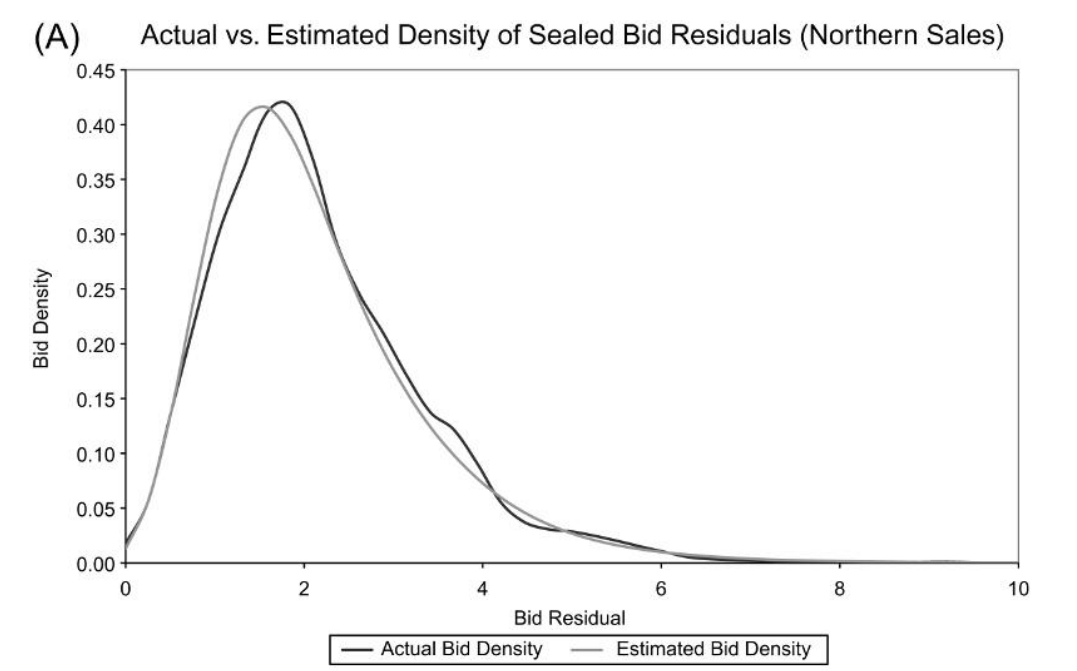
\includegraphics[width=0.49\textwidth]{figures/ch15/als2011_fig1a.png}\hfill
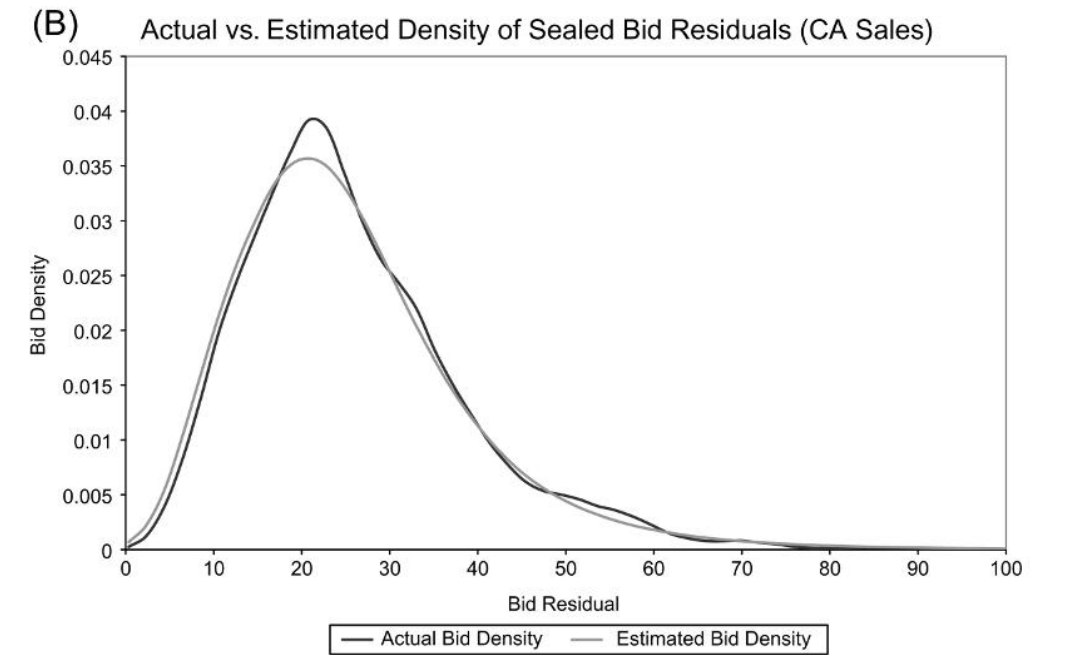
\includegraphics[width=0.49\textwidth]{figures/ch15/als2011_fig1b.png}
\caption{Actual (dark) and model-implied (light) densities of sealed-bid residuals, Northern sales (A)
and California sales (B). Residuals are bids divided by the fitted covariate index, and the actual density
is smoothed with a kernel. Source: \citet{AtheyLevinSeira2011}, Figure I.}
\label{fig:15-als-resid}
\end{figure}

\casehead{Recovering values}
Each sealed bid must be optimal against the rivals' bid distributions. Given $(Z,\omega,\bm N,\bm n)$, the
value behind a bid is given by \eqref{eq:15-als-inverse} \citep[eq.~(9)]{AtheyLevinSeira2011}. For the
Weibull distribution the reverse hazard rate has a closed form. Differentiating
\eqref{eq:15-als-weibull},
\[
g_k(b\mid\omega)=\omega\rho_kb^{\rho_k-1}\lambda_k^{-\rho_k}\exp\Bigl(-\omega\Bigl(\frac{b}{\lambda_k}\Bigr)^{\rho_k}\Bigr).
\]
Dividing by $G_k$ and multiplying numerator and denominator by $\exp(\omega(\frac{b}{\lambda_k})^{\rho_k})$,
\begin{equation}\label{eq:15-als-revhaz}
\frac{g_k(b\mid\omega)}{G_k(b\mid\omega)}=\frac{\omega\rho_kb^{\rho_k-1}\lambda_k^{-\rho_k}}{\exp\bigl(\omega(\frac{b}{\lambda_k})^{\rho_k}\bigr)-1}.
\end{equation}
Truncating the upper tail divides $g_k$ and $G_k$ by the same constant, so \eqref{eq:15-als-revhaz} is
unchanged below the truncation point. If $\omega$ were observed, each bid would map into a value, and the
value distributions would follow as in \cref{sec:15-gpv}. As \citet{Krasnokutskaya2011} observed, we can
still recover the value distributions for any value of $\omega$, because the bid functions are strictly
increasing \citep[eq.~(10)]{AtheyLevinSeira2011}:
\begin{equation}\label{eq:15-als-F}
F_k(v\mid Z,\omega,\bm N)=G_k\bigl(\xi_k^{-1}(v\mid Z,\omega,\bm N,\bm n)\bigm|Z,\omega,\bm N,\bm n\bigr).
\end{equation}

The parameterization implies a scaling property that ALS exploit \citep[p.~243]{AtheyLevinSeira2011}.
Write $s=\exp(Z\bm\theta^\lambda_Z+\bm N\bm\theta^\lambda_N)$, the part of the scale common to both
types, and $\lambda_k=s\tilde\lambda_k(\bm n)$. Then $G_k(b)=\tilde G_k(\frac{b}{s})$, where $\tilde G_k$ is
the distribution at $s=1$. Differentiating, $g_k(b)=\frac{1}{s}\tilde g_k(\frac{b}{s})$, so the reverse
hazard rates scale as $\frac{g_k}{G_k}(b)=\frac{1}{s}\frac{\tilde g_k}{\tilde G_k}(\frac{b}{s})$.
Substituting into \eqref{eq:15-als-inverse},
\[
\xi_i(b)=b+s\Biggl[\sum_{j\in\bm n\setminus i}\frac{\tilde g_j}{\tilde G_j}\Bigl(\frac{b}{s}\Bigr)\Biggr]^{-1}
=s\,\tilde\xi_i\Bigl(\frac{b}{s}\Bigr).
\]
Values, bids and therefore profits all scale with $s$. Profits need to be computed for a single value of
$(Z,\bm N)$ and then rescaled, which makes the many simulations below feasible.

A second property shows how the shape parameters govern market power.

\begin{proposition}[A floor on margins in the Weibull model]\label{prop:15-als-margin}
Under \eqref{eq:15-als-weibull}, for every bid $b>0$, every $\omega$ and every participant set,
\[
\frac{\xi_i(b)-b}{\xi_i(b)}\ \ge\ \frac{1}{1+\sum_{j\in\bm n\setminus i}\rho_j},
\]
with equality in the limit $b\to0$.
\end{proposition}

\begin{proof}
Let $x_j=\omega(\frac{b}{\lambda_j})^{\rho_j}>0$. By \eqref{eq:15-als-revhaz},
$\frac{g_j}{G_j}(b)=\frac{\rho_j}{b}\cdot\frac{x_j}{e^{x_j}-1}$. Since $e^{x}-1>x$ for $x>0$, each factor
$\frac{x_j}{e^{x_j}-1}$ lies in $(0,1)$ and tends to one as $x_j\to0$. Hence
$\sum_j\frac{g_j}{G_j}(b)<\frac{1}{b}\sum_j\rho_j$, and by \eqref{eq:15-als-inverse}
\[
\xi_i(b)-b>\frac{b}{\sum_j\rho_j},\qquad\text{so}\qquad\xi_i(b)>b\,\frac{1+\sum_j\rho_j}{\sum_j\rho_j}.
\]
Write $m=\xi_i(b)-b$. The margin $\frac{m}{b+m}$ increases in $m$, so it exceeds its value at
$m=\frac{b}{\sum_j\rho_j}$, which is $\frac{1}{1+\sum_j\rho_j}$. As $b\to0$, every $x_j\to0$ and the
inequality becomes an equality.
\end{proof}

The proposition is our derivation, not a result in ALS. It shows that the shapes, which measure how
concentrated bids are, discipline the markdowns. With the Northern estimates and two loggers and two mills,
$\rho_L=e^{1.134+2(0.016)+2(0.015)}=3.31$ and $\rho_M=3.56$. Every logger bid in that configuration then
carries a margin of at least $\frac{1}{1+3.31+2(3.56)}=0.088$ (our calculation). ALS estimate the median
profit margin across all bids, averaging over $\omega$, at 9.5 percent in the North and 10.0 percent in
California, similar for mills and loggers \citep[p.~243]{AtheyLevinSeira2011}. The paper does not state
the formula for its margin, so the comparison is only indicative. Margins of this size suggest that sealed
bidding is quite competitive.

\begin{figure}[htbp]
\centering
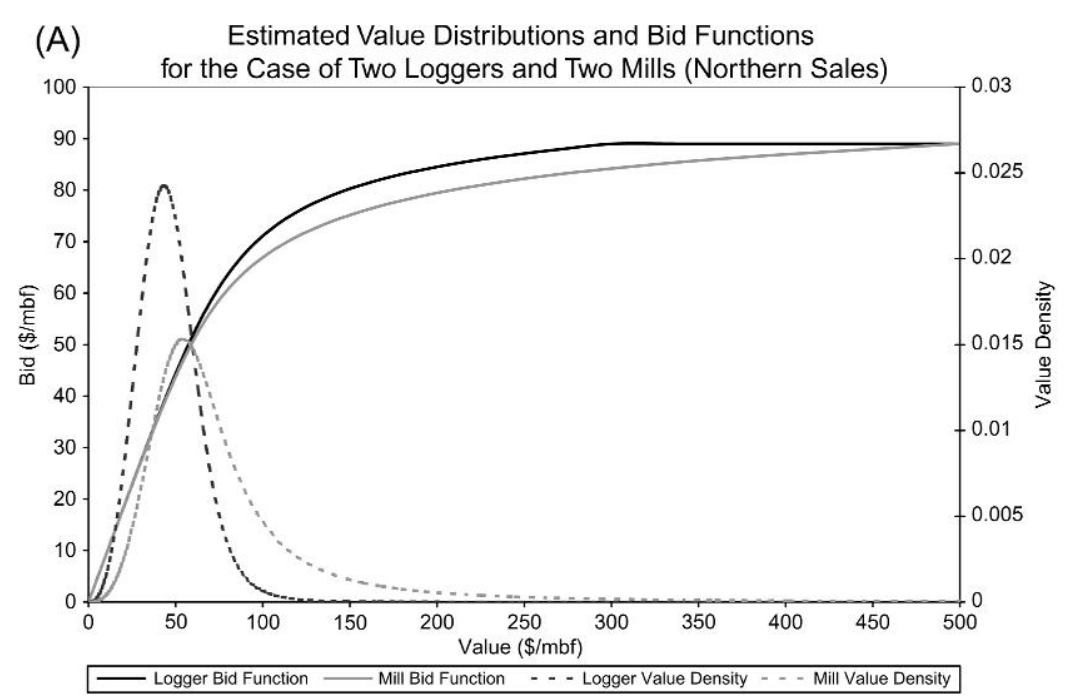
\includegraphics[width=0.49\textwidth]{figures/ch15/als2011_fig2a.png}\hfill
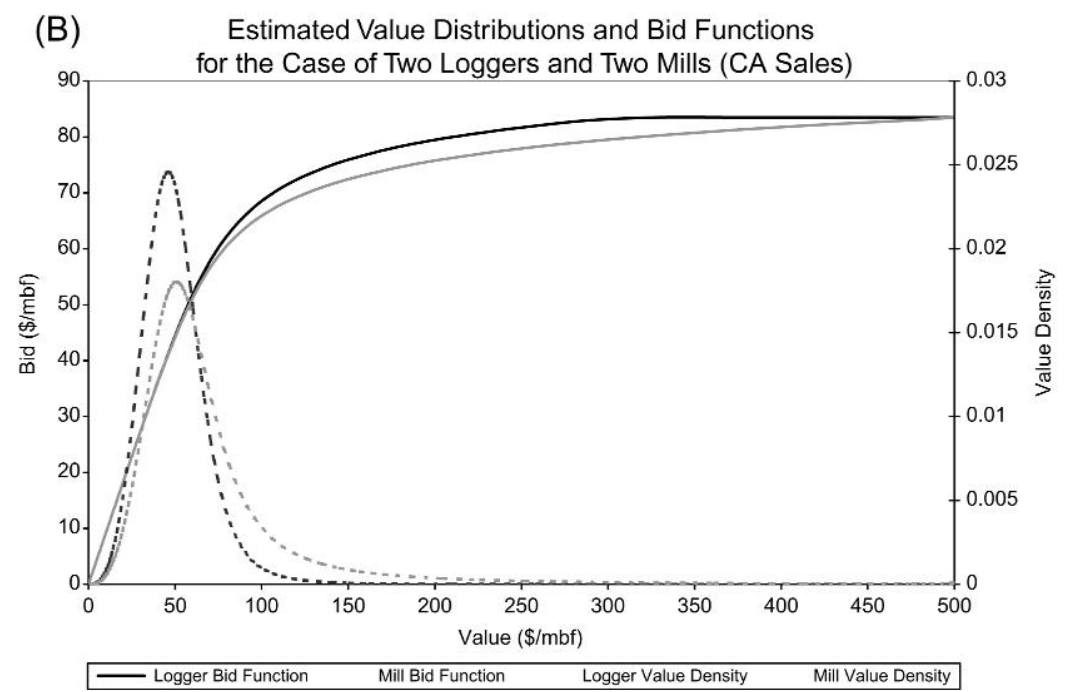
\includegraphics[width=0.49\textwidth]{figures/ch15/als2011_fig2b.png}
\caption{Estimated value densities (dashed, right axis) and equilibrium bid functions (solid, left axis)
for a sale with average covariates, $\omega=1$, two loggers and two mills, Northern sales (A) and California
sales (B). Dark curves are loggers and light curves are mills. The mill value density lies to the right,
and the mill bid function lies below the logger bid function. Source: \citet{AtheyLevinSeira2011},
Figure II.}
\label{fig:15-als-values}
\end{figure}

\Cref{fig:15-als-values} shows the recovered primitives for a sale with average covariates, $\omega=1$ and
two participants of each type. ALS compute the bid functions by inverting $\xi_k$ for the fitted bid
distributions. The mill value distribution is shifted well to the right of the logger distribution. The
mill bid function lies below the logger bid function, so mills bid less than loggers at any given value
(p.~243). This is property (i) of \cref{prop:14-maskin-riley}, the result of \citet{MaskinRiley2000}, now
found in estimated primitives.

\casehead{Checking uniqueness}
Prediction (P2) needs $\pi^{\mathrm s}_M(n_L,n_M+1)>\pi^{\mathrm s}_L(n_L,n_M)$. ALS compute the profits by
simulation \citep[pp.~243--245]{AtheyLevinSeira2011}.
\begin{enumerate}[label=(\arabic*)]
\item Draw $\omega$ from the estimated Gamma distribution.
\item For each participant, draw a bid from $\hat G_L(\cdot\mid\omega)$ or $\hat G_M(\cdot\mid\omega)$.
\item Convert each bid into a value with $\hat\xi_k$ from \eqref{eq:15-als-inverse} and \eqref{eq:15-als-revhaz}.
\item Identify the winner, the highest bidder, and record its profit $v-b$. Losers earn zero.
\item Repeat 5,000 times for each configuration with up to 8 mills and 25 loggers, and average.
\end{enumerate}
The inequality holds for all configurations and every tract in the sample (p.~245). By
\cref{prop:14-als-unique}, the estimated model has a unique type-symmetric entry equilibrium for every
tract, whatever the entry cost. In that equilibrium, if loggers enter with positive probability, every mill
enters.

\casehead{Entry costs}
ALS observe loggers entering 85 percent of Northern sales and 88 percent of California sales (p.~245).
Since potential exceeds actual logger entry almost everywhere, loggers must randomize, and a randomizing
logger is indifferent. For format $\tau$, \citep[eq.~(11)]{AtheyLevinSeira2011}
\begin{equation}\label{eq:15-als-indiff}
\Pi^\tau_L(Z,\bm N)=\sum_{n_L=1}^{N_L}\pi^\tau_L(Z,\bm N,\bm n)\,\Pr\bigl[\bm n\mid Z,\bm N,i\in\bm n,\tau\bigr]=K(Z,\bm N),
\end{equation}
with $n_M=N_M$. This is the general condition \eqref{eq:14-entry-indiff} and the identification argument of
\cref{prop:15-entry-ident}. Given that logger $i$ enters, each of the other $N_L-1$ potential loggers enters
independently with probability $p^\tau(Z,\bm N)$, so \citep[eq.~(12)]{AtheyLevinSeira2011}
\begin{equation}\label{eq:15-als-binom}
\Pr\bigl[n_L\mid Z,\bm N,i\in\bm n,\tau\bigr]=\binom{N_L-1}{n_L-1}p^\tau(Z,\bm N)^{n_L-1}\bigl(1-p^\tau(Z,\bm N)\bigr)^{N_L-n_L}.
\end{equation}
For sealed sales the entry probability is a logit \citep[eq.~(13)]{AtheyLevinSeira2011},
\begin{equation}\label{eq:15-als-logit}
p^{\mathrm s}(Z,\bm N)=\frac{\exp(Z\bm\gamma_Z+\bm N\bm\gamma_N)}{1+\exp(Z\bm\gamma_Z+\bm N\bm\gamma_N)},
\end{equation}
where ALS write $\alpha$ for $\bm\gamma$. In sale $t$ the number of entering loggers is binomial with
$N_{L,t}$ trials and success probability $p_t=p^{\mathrm s}(Z_t,\bm N_t)$. Up to a constant, the
log-likelihood is
\begin{equation}\label{eq:15-als-loglik}
\ln L(\bm\gamma)=\sum_{t\,\in\,\text{sealed}}\Bigl[n_{L,t}\ln p_t+\bigl(N_{L,t}-n_{L,t}\bigr)\ln(1-p_t)\Bigr].
\end{equation}
Let $\bm x_t=(Z_t,\bm N_t)$ be the row of regressors. For the logit, $\frac{\partial\ln p_t}{\partial\bm\gamma}=(1-p_t)\bm x_t^\T$ and
$\frac{\partial\ln(1-p_t)}{\partial\bm\gamma}=-p_t\bm x_t^\T$. The score is therefore
\[
\frac{\partial\ln L}{\partial\bm\gamma}=\sum_t\Bigl[n_{L,t}(1-p_t)-(N_{L,t}-n_{L,t})p_t\Bigr]\bm x_t^\T=\sum_t\bigl(n_{L,t}-N_{L,t}p_t\bigr)\bm x_t^\T .
\]
The maximum likelihood estimator sets the sum of observed minus expected entrants, weighted by the
covariates, to zero. The estimates are the entry columns of \cref{tab:15-als-estimates}.

The entry cost then follows without further estimation. ALS combine the simulated profits
$\hat\pi^{\mathrm s}_L(Z,\bm N,\bm n)$ with $\hat p^{\mathrm s}(Z,\bm N)$ in
\eqref{eq:15-als-indiff} and \eqref{eq:15-als-binom}, and set $\hat K(Z,\bm N)=\hat\Pi^{\mathrm s}_L(Z,\bm N)$ for each
tract. The median entry cost is \$2,870 (s.e.\ \$325) in the North and \$5,056 (s.e.\ \$673) in California
\citep[p.~246]{AtheyLevinSeira2011}. Cruising a tract can cost several thousand dollars, so these figures
are plausible. For comparison, the median expected profit of a mill in a sealed sale is roughly \$45,000
gross of entry costs (footnote 26). The median entry costs are thus about 6.4 and 11.2 percent of that
profit, the ratios reported by \citet[p.~91]{HortacsuPerrigne2021} (\cref{tab:15-entry-costs}). Two checks support the specification. If loggers entered with
probability zero in some tracts, the data would contain significantly more sales without logger entry than
the binomial model predicts, and they do not (footnote 25). Under pure-strategy entry, revealed preference
gives fairly tight bounds on entry costs that are similar to the point estimates (footnote 26).

\Cref{fig:15-als-entry} illustrates the logic and anticipates the open-auction prediction. The logger's
entry payoff falls with the probability that other loggers enter. A logger earns less in an open auction
for any participant set, so the open curve lies below the sealed curve. With the cost $K$ fixed, the
equilibrium entry probability is lower under open bidding.

\begin{figure}[htbp]
\centering
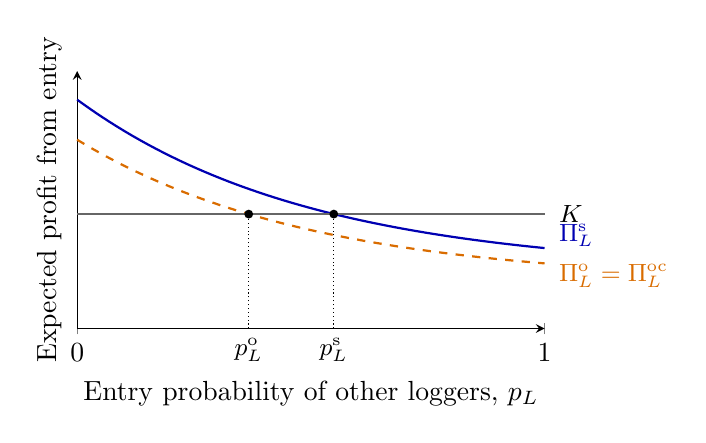
\begin{tikzpicture}
\begin{axis}[
  width=0.62\textwidth, height=0.40\textwidth,
  xmin=0, xmax=1, ymin=0, ymax=9,
  xlabel={Entry probability of other loggers, $p_L$},
  ylabel={Expected profit from entry},
  axis lines=left, xtick={0,1}, ytick=\empty,
  clip=false, every axis plot/.append style={thick}]
\addplot[domain=0:1, samples=60, blue!70!black] {2+6*exp(-2*x)};
\addplot[domain=0:1, samples=60, orange!85!black, dashed] {1.6+5*exp(-2*x)};
\addplot[domain=0:1, samples=2, black!60] {4};
\node[anchor=west, font=\small, blue!70!black] at (axis cs:1.01,3.25) {$\Pi^{\mathrm s}_L$};
\node[anchor=west, font=\small, orange!85!black] at (axis cs:1.01,1.85) {$\Pi^{\mathrm o}_L=\Pi^{\mathrm{oc}}_L$};
\node[anchor=west, font=\small] at (axis cs:1.01,4) {$K$};
\draw[densely dotted] (axis cs:0.549,0) -- (axis cs:0.549,4);
\draw[densely dotted] (axis cs:0.367,0) -- (axis cs:0.367,4);
\fill (axis cs:0.549,4) circle (1.6pt);
\fill (axis cs:0.367,4) circle (1.6pt);
\node[below, font=\small] at (axis cs:0.549,0) {$p^{\mathrm s}_L$};
\node[below, font=\small] at (axis cs:0.367,0) {$p^{\mathrm o}_L$};
\end{axis}
\end{tikzpicture}
\caption{Logger entry in the type-symmetric equilibrium with $p_M=1$ (schematic, not estimated). The
entry payoff of a logger falls in the entry probability of the other loggers. Indifference with the entry
cost $K$ pins down $p^{\mathrm s}_L$ in sealed auctions and the lower $p^{\mathrm o}_L$ in open auctions.
Mill collusion in open auctions leaves logger profits unchanged ($\Pi^{\mathrm{oc}}_L=\Pi^{\mathrm o}_L$),
so it leaves logger entry unchanged.}
\label{fig:15-als-entry}
\end{figure}

\subsection{Out-of-sample predictions and the competitiveness of open auctions}\label{sec:15-als-predict}

With the value distributions and entry costs in hand, ALS predict the outcome of every sale and compare
the predictions with the data \citep[pp.~247--248]{AtheyLevinSeira2011}. The procedure has four parts.
\begin{enumerate}[label=(\arabic*)]
\item \emph{Sealed sales.} The entry logit gives the distribution of entering loggers, and mill entry is
known. The fitted bid distributions, integrated over $\omega$, give bidding outcomes for each participant
set. Combining the two gives outcomes conditional on the tract characteristics alone.
\item \emph{Open sales, competitive.} For each simulated auction, draw $\omega$ and draw a value for each
participant from $\hat F_L(\cdot\mid Z,\omega,\bm N)$ or $\hat F_M(\cdot\mid Z,\omega,\bm N)$ via
\eqref{eq:15-als-F}. Then record the price $P^{\mathrm o}=\max\{V^{(n-1:n)},r\}$, the second-highest
participant value or the reserve price.
\item \emph{Open sales, collusive.} All participating mills except the one with the highest value drop out
at once. The price is the second-highest value in the set formed by the top mill and the loggers, or the
reserve price.
\item \emph{Open entry.} Mill entry equals the potential mill count. The logger entry probability
$p^{\mathrm o}_L$ is the unique solution of $\hat\Pi^{\mathrm o}_L(Z,\bm N;p_L)=\hat K(Z,\bm N)$. Uniqueness
holds because $\hat\Pi^{\mathrm o}_L$ falls monotonically in $p_L$ \citep[footnote 27]{AtheyLevinSeira2011}.
By prediction (P5), the same $p^{\mathrm o}_L$ applies under collusion.
\end{enumerate}
Standard errors come from a parametric bootstrap. ALS draw parameters from the estimated asymptotic
distribution of the \cref{tab:15-als-estimates} estimates and repeat the whole calculation for each draw
(p.~248). Column (2) of \cref{tab:15-als-predict} conditions on the observed participants, and column (3)
predicts entry as well.

\begin{table}[htbp]
\centering
\caption{Actual outcomes and outcomes predicted by the estimated model}
\label{tab:15-als-predict}
\small
\begin{tabular}{@{}lrccc@{}}
\toprule
 & $N$ & (1) Actual & (2) Predicted, & (3) Predicted,\\
 & & & bidding only & bidding and entry\\
\midrule
\multicolumn{5}{@{}l}{\textit{A. Northern sales}}\\
\multicolumn{5}{@{}l}{\quad Sealed-bid sales}\\
\quad Average bid & 1,492 & 59.6 & 58.2 (1.4) & 57.4 (1.3)\\
\quad Average logger bid & 1,096 & 50.8 & 48.7 (1.4) & 47.4 (1.4)\\
\quad Average mill bid & 396 & 83.8 & 84.7 (2.7) & 85.2 (2.7)\\
\quad Average sale price & 339 & 69.4 & 69.9 (1.4) & 70.4 (1.6)\\
\quad Average revenue (thousands) & 339 & 111.4 & 108.1 (4) & 109.9 (4.2)\\
\quad Percent of sales won by loggers & 339 & 68.1 & 68.0 (0.90) & 65.0 (0.01)\\
\quad Average logger entry & 339 & 3.23 & & 3.23 (0.09)\\
\multicolumn{5}{@{}l}{\quad Open auction sales}\\
\quad Average sale price, competition & 732 & 63.3 & 67.9 (1.8) & 67.8 (2.1)\\
\quad Average sale price, collusion & 732 & 63.3 & 44.2 (1.3) & 44.1 (2.2)\\
\quad Average revenue, competition & 732 & 144.7 & 152.7 (6.8) & 154.8 (7.9)\\
\quad Average revenue, collusion & 732 & 144.7 & 61.0 (2) & 64.7 (5.0)\\
\quad Percent of sales won by loggers & 732 & 59.0 & 56.0 (0.01) & 54.4 (0.02)\\
\quad Average logger entry & 732 & 2.75 & & 2.67 (0.17)\\[3pt]
\multicolumn{5}{@{}l}{\textit{B. California sales}}\\
\multicolumn{5}{@{}l}{\quad Sealed-bid sales}\\
\quad Average bid & 1,630 & 73.6 & 74.7 (2.3) & 74.2 (2.3)\\
\quad Average logger bid & 1,150 & 64.0 & 63.6 (2.1) & 62.3 (2.4)\\
\quad Average mill bid & 480 & 96.5 & 101.2 (3.5) & 102.8 (3.8)\\
\quad Average sale price & 382 & 80.4 & 83.8 (2.1) & 84.4 (2.4)\\
\quad Average revenue (thousands) & 382 & 103.1 & 110.7 (3.8) & 111.9 (4.0)\\
\quad Percent of sales won by loggers & 382 & 66.8 & 66.4 (1.2) & 62.6 (1.3)\\
\quad Average logger entry & 382 & 3.01 & & 3.01 (0.07)\\
\multicolumn{5}{@{}l}{\quad Open auction sales}\\
\quad Average sale price, competition & 325 & 85.1 & 87.2 (2.7) & 86.7 (3.1)\\
\quad Average sale price, collusion & 325 & 85.1 & 46.1 (1.2) & 51.0 (1.6)\\
\quad Average revenue, competition & 325 & 227.0 & 244.7 (9.7) & 242.4 (10.9)\\
\quad Average revenue, collusion & 325 & 227.0 & 93.2 (2.6) & 112.9 (5.6)\\
\quad Percent of sales won by loggers & 325 & 50.5 & 48.2 (1.1) & 43.6 (1.8)\\
\quad Average logger entry & 325 & 1.95 & & 1.90 (0.13)\\
\bottomrule
\end{tabular}

\smallskip
\begin{minipage}{\linewidth}
\footnotesize\textit{Notes.} Reproduced from \citet[Table V]{AtheyLevinSeira2011}. Bids and prices in 1982
dollars per mbf, revenue in thousands of 1982 dollars. Column (1) shows average outcomes. Column (2) shows
predictions for the same sales conditional on the observed entrants. Column (3) shows predictions of the
equilibrium model of entry and bidding. Parametric bootstrap standard errors in parentheses, as printed
(the paper prints a second standard error, 0.1, below the row for Northern sealed-bid logger entry). The
standard errors for the percent of sales won by loggers appear in mixed units in the original.
\end{minipage}
\end{table}

\casehead{In-sample fit}
The sealed-bid rows measure fit, since these sales were used in estimation. In the North the average sale
price is 69.4 dollars per mbf, against predictions of 69.9 with observed entry and 70.4 with predicted
entry \citep[p.~248]{AtheyLevinSeira2011}. Average logger and mill bids and the share of sales won by
loggers are also close. The largest discrepancy is in California, where the model overpredicts the sale
price, 84.4 or 83.8 against 80.4, and the revenue.

\casehead{Out-of-sample entry and allocation}
The open-auction rows are the demanding test. The model predicts open-auction logger entry of 2.67 in the
North against 2.75 observed, and 1.90 in California against 1.95 \citep[p.~250]{AtheyLevinSeira2011}. The
model therefore explains the entry gap between formats, one of the main departures from revenue
equivalence. It is less successful with allocation. It predicts that loggers win 54.4 percent of Northern
open sales, or 56.0 percent with observed entry, against 59.0 percent observed. California shows a similar
underprediction.

\casehead{Out-of-sample prices and conduct}
In California the competitive model predicts an open-auction price of 87.2 with observed entry and 86.7
with predicted entry, against 85.1 observed. The model reproduces the absence of a price difference between
formats. The North is different. The competitive model predicts 67.9 or 67.8, and the fully collusive model
44.2 or 44.1. The observed average is 63.3. Accounting for sampling error, ALS reject both models at
conventional levels. ``Mildly cooperative'' behavior by participating mills fits better than either extreme
(pp.~250--251). A linear interpolation between the competitive and collusive predictions in column (2)
gives a cooperation share of $\frac{67.9-63.3}{67.9-44.2}=0.19$ (our calculation). ALS use 18 percent as the
share that rationalizes Northern open prices in their welfare analysis.

Two robustness arguments strengthen the conclusion (p.~251). If sealed bidding were partly collusive, the
inferred values would be higher, and open prices would look even less competitive. ALS also examined the
open sales whose predicted price lies far above the actual price and found no obvious pattern.

\casehead{Where collusion should show up}
Statistical detection of collusion is hard \citep{BajariYe2003}, so ALS test a sharper implication of
(P5). With zero or one participating mill the competitive and collusive models predict the same price.
Any effect of mill collusion must appear in sales with two or more mills.
\Cref{tab:15-als-mills,fig:15-als-mills} split the Northern sales by mill participation.

\begin{table}[htbp]
\centering
\caption{Actual and predicted sale prices by mill participation, Northern sales}
\label{tab:15-als-mills}
\small
\begin{tabular}{@{}lrccc@{}}
\toprule
 & $N$ & (1) Actual & (2) Predicted, & (3) Predicted,\\
 & & & bidding only & bidding and entry\\
\midrule
\multicolumn{5}{@{}l}{\textit{Zero mills}}\\
\quad Sealed-bid sales & 181 & 51.7 & 51.4 & 51.4\\
\quad Open auction sales & 321 & 49.8 & 50.5 & 47.1\\
\multicolumn{5}{@{}l}{\textit{One mill}}\\
\quad Sealed-bid sales & 70 & 66.8 & 64.6 & 66.9\\
\quad Open auction sales & 150 & 50.0 & 52.2 & 59.5\\
\multicolumn{5}{@{}l}{\textit{Two or more mills}}\\
\quad Sealed-bid sales & 88 & 108.1 & 112.1 & 112.2\\
\quad Open auction sales & 261 & 87.5 & 98.5 & 98.0\\
\bottomrule
\end{tabular}

\smallskip
\begin{minipage}{0.84\linewidth}
\footnotesize\textit{Notes.} Reproduced from \citet[Table VI]{AtheyLevinSeira2011}. Average sale prices
in 1982 dollars per mbf. Predictions assume competitive bidding.
\end{minipage}
\end{table}

\begin{figure}[htbp]
\centering
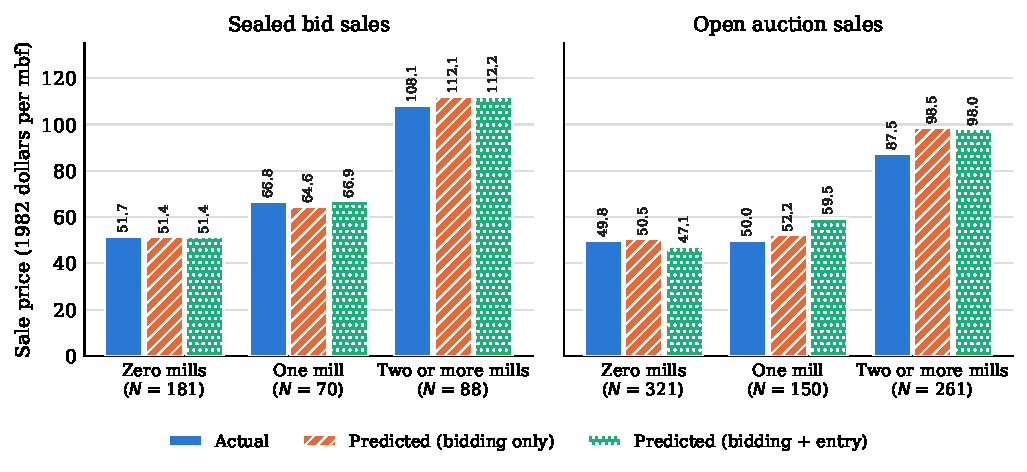
\includegraphics[width=0.92\textwidth]{figures/ch15/als_tableVI.pdf}
\caption{Actual and predicted competitive sale prices by mill participation, Northern sales. Drawn from
the numbers in \citet[Table VI]{AtheyLevinSeira2011}. With observed entry, the competitive model fits open prices
with zero or one mill and overpredicts them with two or more mills.}
\label{fig:15-als-mills}
\end{figure}

With exogenous entry, column (2), the competitive model predicts open prices accurately with zero mills
(50.5 against 49.8) and one mill (52.2 against 50.0). With two or more mills it predicts 98.5 against an
observed 87.5, a shortfall of 11 percent (our calculation), as the collusion theory implies
\citep[p.~252]{AtheyLevinSeira2011}. In sealed sales with two or more mills the shortfall is 4 percent.
Column (3) is less sharp, because the model does not fit realized logger entry cell by cell. For open sales
it predicts 3.31, 2.26 and 1.06 entering loggers in sales with zero, one and two or more mills, against
3.76, 3.32 and 1.77 observed (footnote 28). Column (2) uses observed entry and isolates the bidding margin.
Since the theory predicts identical entry under competition and collusion, that margin is where the two
hypotheses differ.

\subsection{Counterfactual comparison of formats}\label{sec:15-als-welfare}

ALS finally take the estimates as the true primitives and ask what would happen if every tract were sold by
one format \citep[Section V.C]{AtheyLevinSeira2011}. For each tract and format they compute expected entry,
the expected price and revenue, the probability that a logger wins and the expected surplus. Surplus is the
winner's value net of the entry costs sunk by all participants. Under exogenous entry, participation is
fixed at its realized value. Under endogenous entry, both formats are solved for their entry equilibria.
For open auctions they consider competitive mills and mills that cooperate 18 percent of the time.
\Cref{tab:15-als-welfare} reproduces the results.

\begin{table}[htbp]
\centering
\caption{Counterfactual outcomes of sealed and open auctions}
\label{tab:15-als-welfare}
\small
\setlength{\tabcolsep}{4.5pt}
\begin{tabular}{@{}lccccc@{}}
\toprule
 & (1) & (2) & (3) & (4) & (5)\\
 & Sealed & Open & Sealed $-$ open & Open & Sealed $-$ open\\
 & & (competitive) & (1) $-$ (2) & (partly collusive) & (1) $-$ (4)\\
\midrule
\multicolumn{6}{@{}l}{\textit{A. Northern sales ($N=1{,}071$)}}\\
\multicolumn{6}{@{}l}{\quad Exogenous entry}\\
\quad Average sale price & 68.56 & 68.53 & 0.03 (0.04) & 64.58 & 3.98 (0.24)\\
\quad Average revenue & 138.33 & 138.64 & $-0.32$ (0.06) & 124.33 & 14.00 (1.22)\\
\quad Average surplus & 176.99 & 177.06 & $-0.08$ (0.02) & & \\
\quad Percent won by loggers & 60.14 & 59.68 & 0.46 (0.16) & & \\
\multicolumn{6}{@{}l}{\quad Endogenous entry}\\
\quad Average sale price & 69.68 & 68.19 & 1.49 (0.71) & 64.11 & 5.57 (0.82)\\
\quad Average revenue & 143.04 & 139.87 & 3.17 (2.24) & 125.32 & 17.72 (2.74)\\
\quad Average surplus & 156.53 & 156.84 & $-0.30$ (2.70) & & \\
\quad Percent won by loggers & 59.65 & 57.19 & 2.46 (0.00) & & \\
\quad Logger entry & 3.10 & 2.76 & 0.34 (0.12) & & \\[3pt]
\multicolumn{6}{@{}l}{\textit{B. California sales ($N=707$)}}\\
\multicolumn{6}{@{}l}{\quad Exogenous entry}\\
\quad Average sale price & 85.53 & 85.20 & 0.32 (0.07) & 79.39 & 6.13 (0.39)\\
\quad Average revenue & 172.64 & 172.10 & 0.55 (0.13) & 154.43 & 18.21 (1.36)\\
\quad Average surplus & 203.61 & 203.65 & $-0.04$ (0.02) & & \\
\quad Percent won by loggers & 58.21 & 57.81 & 0.40 (0.002) & & \\
\multicolumn{6}{@{}l}{\quad Endogenous entry}\\
\quad Average sale price & 88.36 & 83.76 & 4.60 (2.26) & 78.55 & 9.81 (2.21)\\
\quad Average revenue & 182.38 & 168.20 & 14.18 (5.43) & 152.83 & 29.55 (5.39)\\
\quad Average surplus & 181.82 & 170.58 & 11.24 (6.86) & & \\
\quad Percent won by loggers & 55.84 & 52.66 & 3.18 (0.01) & & \\
\bottomrule
\end{tabular}

\smallskip
\begin{minipage}{\linewidth}
\footnotesize\textit{Notes.} Reproduced from \citet[Table VII]{AtheyLevinSeira2011}. Averages over all
tracts in a region of model predictions. Prices in 1982 dollars per mbf, revenue and surplus in thousands
of 1982 dollars. Exogenous entry uses the realized participants, and endogenous entry uses the equilibrium
entry model. The partly collusive open auction has mills cooperating 18 percent of the time. Bootstrap
standard errors in parentheses. The text of the paper (p.~253) states that with fixed participation sealed
bidding raises Northern revenue by \$320 per sale. The table prints a difference of $-0.32$ thousand,
consistent with its columns (1) and (2).
\end{minipage}
\end{table}

\casehead{A discrepancy in the source}
With fixed participation, the text of ALS reports a sealed-bid revenue gain of ``only \$320 per sale in
the Northern region and \$546 in California'' (p.~253).
Table VII prints a Northern difference of $-0.32$ thousand dollars. The table's own columns agree with the
negative sign, since $138.33-138.64=-0.31$. For California the text and table agree, $0.55$ thousand. We
report the table and conclude that with fixed participation the Northern revenue difference is a few
hundred dollars, of uncertain sign as printed.

\casehead{Lessons}
Four lessons emerge \citep[pp.~253--255]{AtheyLevinSeira2011}.
\begin{enumerate}[label=(\roman*)]
\item \emph{With fixed participation and competitive bidding, the format barely matters.} Revenue
differences are a few hundred dollars per sale, and the logger win probability changes by less than one
percentage point. The efficiency advantage of the open auction is under \$100 per sale in both regions.
The asymmetry between mills and loggers is substantial, yet its consequences for fixed participants are
small.
\item \emph{Entry magnifies the differences.} Both formats attract the same mills, but sealed bidding
attracts three to four more loggers per 10 sales (0.34 more per sale in the North). Loggers win 2 to 4
percentage points more sales. The sealed-bid revenue advantage rises to roughly \$3,000 per sale in the
North and \$14,000 in California, which is 2.3 and 8.4 percent of competitive open-auction revenue (our
calculation).
\item \emph{Efficiency comparisons are noisy.} The surplus difference stays small in the North. In
California the point estimate even favors sealed bidding, although sealed bidding is known to be less
efficient in equilibrium. The reason is that ALS estimate separate value distributions for each
participant configuration, and these estimates are not identical. Expectations over stochastic logger
entry weight the configurations differently across formats (footnote 29). Pooling the configurations would
break the link between the value distribution and the estimated bid distribution through the first-order
condition.
\item \emph{Collusion dominates.} Suppose mills cooperate 18 percent of the time in open auctions. Open bidding
then raises about \$14,000 less per Northern sale than competitive sealed bidding with fixed participation,
and over \$17,000 less with entry effects. The California differences are larger, \$18,210 and \$29,550 in
\cref{tab:15-als-welfare}.
\end{enumerate}
The revenue consequences of the format choice run mainly through the vulnerability of open auctions to
collusion. Gains from extra logger entry come second, and efficiency losses are small.

\subsection{Assessment}\label{sec:15-als-assessment}

\casehead{Contribution}
ALS combine three features that earlier work had treated separately: asymmetric bidders, unobserved
auction heterogeneity and endogenous participation \citep[p.~255]{AtheyLevinSeira2011}. Their entry model
recovers entry costs in dollars from post-entry profits and observed entry rates. Earlier entry models in
industrial organization infer profits relative to a normalized distribution of entry costs. Their main
methodological idea is to use variation in the rules for validation. The parameters come from one game and
are tested on another, which is a demanding out-of-sample check. The logic resembles the validation of
conduct estimates against direct cost data in \cref{ch:conduct}, with the second auction format in place of
the cost data. The approach also yields a conduct test. Behavior in the format least prone to collusion
serves as a benchmark for behavior in the format where collusion is suspected.

\casehead{Limitations}
Several assumptions deserve scrutiny.
\begin{itemize}
\item \emph{Functional form.} The Weibull and Gamma forms and the independence of $\omega$ from $Z$ are
maintained hypotheses. They pass an informal moment check and a formal specification test, but they drive
the extrapolation to open auctions. \citet{Roberts2013} argues that the reserve price itself carries
information about $\omega$ (\cref{sec:15-uh}). ALS include the reserve price in $Z$, so this would violate
the independence of $\omega$ and $Z$, and the large reserve-price coefficient in \cref{tab:15-als-estimates}
may partly proxy for $\omega$.
\item \emph{Competitive sealed bidding.} The benchmark assumes that sealed bidding is competitive. ALS
argue that sealed collusion would only strengthen the conclusion, but a cartel operating in both formats
would weaken the cross-format test.
\item \emph{Two types and a crude model of collusion.} Bidders are mills or loggers, and collusion is
modeled as perfect mill cooperation in a fraction of sales. Partial cooperation, cooperation that depends
on the identities of the mills, or coordinated entry would change the predictions.
\item \emph{Entry.} Point identification of entry costs relies on type-symmetric mixed strategies and on
the measured number of potential loggers, which contains error. Values learned only after entry rule out
selective entry.
\item \emph{Format selection.} In California the format varies strongly with size, and trimming keeps one
third of the sales. Selection on unobservables remains a concern there.
\item \emph{Open auctions as button auctions.} Open predictions assume that the price equals the
second-highest value. Jump bidding and bid increments break this equality (\cref{thm:15-ht}).
\item \emph{Two-step consistency.} Value distributions estimated separately by participant set need not
coincide, which produces the anomalous California surplus estimate.
\end{itemize}

\casehead{Follow-up work}
Later studies of Forest Service sales build on this model \citep[Section~2.6]{HortacsuPerrigne2021}.
\citet{AtheyCoeyLevin2013} evaluate small-business set-asides, sales reserved for firms with fewer than 500
employees. Their model keeps the entry and the mill-logger asymmetry of ALS and uses California's open and
sealed sales. Opening the set-aside sales to large firms would cut the share of sales won by small firms by
51 percent. It would raise revenue by 6 percent and surplus by 21 percent (pp.~98--99). A bid subsidy of
only 5 or 6 percent for small firms would keep their share of sales satisfactory. Prices would then rise by
4 percent and efficiency by 2 percent. \citet{RobertsSweeting2013} let bidders receive signals of their
values before entry, which makes entry selective. They compare the simultaneous open auction with a
sequential mechanism. In it, entrants arrive one at a time, observe the earlier offers and may jump bid to
deter later entry. With moderate selection and an entry cost of 2 percent of the average winning bid, the
sequential mechanism raises revenue by 1.8 percent. A simultaneous auction with an optimal reserve raises
it by 0.2 percent (pp.~99--100). \citet{Haile2001} studies resale. When winners can resell in a secondary
market, the values at which bidders drop out of an open auction rise with the number of bidders. Common
values predict the reverse, through the winner's curse. He instruments the number of bidders with the number
of sawmills in and near the county, and the evidence supports the model with resale (p.~100). The bounds of
\citet{AradillasLopezGandhiQuint2013} for correlated private values are applied to Oregon sales in
\cref{sec:15-reserve-asc}.

\section{Testing for Collusion with Auction Data}\label{sec:15-collusion}

Auction data seem ideal for detecting collusion. The rules are known, every bid and bidder is often
recorded, and the competitive benchmark is a fully specified game. Detection is nonetheless hard.
\citet{PorterZona1993}, in the working-paper version we follow, explain why.\footnote{We use NBER Working
Paper 4013 (March 1992) for the description of the tests. The published estimates are discussed in
\cref{sec:13-detection}.} Patterns often read as collusion can arise in competitive equilibria. Rotating
winners are consistent with competition when firms face capacity constraints. Comparisons of winning bids
with engineers' cost estimates can mislead, because the estimates may be inflated by past bids. Collusive
schemes take many forms \citep{HendricksPorter1989}. A cartel might rotate a single bid among its members,
or several members might submit higher \emph{complementary bids}, also called \emph{phantom bids}, to
create the appearance of competition. No single test can detect every scheme. A cartel that includes every
bidder could even choose complementary bids that pass any broadly applicable test. Its bids would mimic
competitive bids for some plausible realization of costs (Porter and Zona, working paper, pp.~2--3).

\citet[p.~211]{AtheyLevinSeira2011} sort the empirical approaches into three groups.
\Cref{tab:15-collusion-tests} summarizes them. The first group requires prior knowledge of the cartel's
existence and structure and compares suspected members with other bidders. The second derives in-sample
specification tests of the competitive model and treats collusion as the alternative. The third, which ALS
introduce, uses behavior under one format as the benchmark for another.

\begin{table}[htbp]
\centering
\caption{Approaches to detecting collusion with auction data}
\label{tab:15-collusion-tests}
\footnotesize
\begin{tabularx}{\linewidth}{@{}>{\raggedright\arraybackslash}p{2.3cm}>{\raggedright\arraybackslash}X>{\raggedright\arraybackslash}X>{\raggedright\arraybackslash}p{2.6cm}@{}}
\toprule
Approach & Maintained information & Implication tested & Examples\\
\midrule
Suspected members versus others & Identity of a candidate cartel, bid levels and ranks & Determinants of
non-winning cartel bids differ from those of the low cartel bid and of non-cartel bids & \citet{PorterZona1993,PorterZona1999}\\
\addlinespace
Specification tests of competition & Bidder and auction covariates & Conditional independence and
exchangeability of bids & \citet{BajariYe2003}\\
\addlinespace
Cross-format benchmark & A format presumed competitive & Prices in the suspect format fall short of
predictions only where theory says collusion bites & \citet{AtheyLevinSeira2011}\\
\addlinespace
Records of a known cartel & Knockout bids and side payments & Structural values and damages from the
cartel's internal bids & \citet{Asker2010}\\
\addlinespace
Super-plus factors & Bid histories, registrations, ownership after the sale & Transfers among bidders, no
rivalry within a subset, prompt resale, close losing bids & \citet{MarshallMarx2012}\\
\bottomrule
\end{tabularx}
\end{table}

\casehead{Porter and Zona: low cartel bids versus higher cartel bids}
Porter and Zona study state highway paving contracts on Long Island in the early 1980s. A set of five firms,
named in a bid-rigging conviction and related suits, forms a candidate cartel. Insiders described meetings
that designated a serious bidder and its bid, after which other members submitted higher bids. The cartel
did not rotate single bids. Several members bid on most jobs, which makes detection possible because ring
behavior can be compared with that of non-members. Each competitive bidder in a low-bid procurement auction
chooses its bid $b$ to maximize $(b-c_{it})\Psi_{it}(b)$, where $c_{it}$ is its cost on job $t$ and
$\Psi_{it}(b)$ its probability of submitting the lowest bid. The first-order condition is
\[
\Psi_{it}(b)+(b-c_{it})\Psi_{it}'(b)=0 ,
\]
the procurement analog of \eqref{eq:15-als-foc}. Costs are unobserved, so Porter and Zona approximate the
equilibrium bid by a log-linear rule,
\begin{equation}\label{eq:15-pz-bid}
\ln B_{it}=\alpha_t+W_{it}\bm\vartheta+\epsilon_{it},\qquad\E[\epsilon_{it}]=0,\qquad\Var(\epsilon_{it})=\sigma_t^2 .
\end{equation}
Here $\alpha_t$ is a job effect, $W_{it}$ are firm-job cost shifters such as capacity and backlog, and
$\epsilon_{it}$ is private cost information whose variance differs by job. Ordinary least squares on competitive bids
estimates $\bm\vartheta$, the job mean squared residual estimates $\sigma_t^2$, and feasible generalized
least squares reweights the data.

The sharper test uses the ranking of bids. Let $X_{it}=-\frac{W_{it}}{\hat\sigma_t}$ be the deflated cost
shifters with the sign reversed. If $-\epsilon_{it}$ is type I extreme value, the job effect cancels and the
probability that firm $i$ submits the lowest bid takes the logit form. The probability of the observed
ranking $b_{r_1t}<b_{r_2t}<\dots<b_{r_nt}$ is the rank-ordered logit
\begin{equation}\label{eq:15-pz-rank}
\Pr\bigl[b_{r_1t}<\dots<b_{r_nt}\bigr]=\prod_{m=1}^{n-1}\frac{\exp(\bm\vartheta X_{r_mt})}{\sum_{l=m}^{n}\exp(\bm\vartheta X_{r_lt})} .
\end{equation}
The likelihood factors into the probability of the lowest bid and the probabilities of the ranks above it.
Under correct specification and no phantom bidding, both parts carry the same coefficients. A likelihood
ratio test applied to competitive bids checks the specification. The same test applied to cartel bids
asks whether the low cartel bid and the higher cartel bids share determinants. Complementary bids are not
meant to win, so their ranking need not reflect cost differences. Porter and Zona find that ranks and
levels of non-cartel bids follow cost measures, while the ranks of higher cartel bids do not and differ
from those of the low cartel bid. A Chow test of a common bid equation for cartel and competitive firms, estimated as in their Table~4,
gives $F(76,319)=9.38$ (p.~33). For competitive bids, the likelihood ratio statistic for equal coefficients
across ranks is $4.30$ against a $\chi^2_6$ distribution, a $p$-value of $0.64$ (p.~33, estimates in Table~5).
For cartel bids it is $8.94$ against a $\chi^2_4$ distribution, a $p$-value of $0.063$ (p.~34, estimates in
Table~6). The $p$-values are our
computation. Page and table numbers refer to the NBER working-paper version of \citet{PorterZona1993}, and
\cref{sec:13-detection} reports the full estimates.

\casehead{Bajari and Ye: independence and exchangeability}
A second approach needs no list of suspects. In an independent private values model with symmetric
bidders, bids are independent across bidders conditional on the covariates, and the joint distribution of
bids is exchangeable \citep[Section 5.5]{AtheyHaile2007}. Suppose values have the form
$V_{it}=h(Z_{1t},Z_{2i},Z_{2(-i)},A_{it})$, where $Z_{1t}$ is an auction covariate, $Z_{2i}$ a bidder
covariate, $Z_{2(-i)}$ the rivals' covariates and $A_{it}$ an idiosyncratic factor with an exchangeable
distribution. Each bid then depends on $(Z_{1t},Z_{2i},Z_{2(-i)})$ and not on the bidder's identity. Two
regression tests follow. Residuals from regressions of bids on covariates should be uncorrelated across
bidders, and coefficients should be equal across bidders or classes of bidders.
\citet{BajariYe2003} apply both tests to highway construction procurement. Collusion is the alternative.
Rejection can also reflect omitted heterogeneity common to the bidders, the problem of \cref{sec:15-uh}.

\casehead{The structural signature}
ALS add a third approach with three steps. Estimate the model on the segment least prone to collusion,
sealed sales. Predict outcomes where collusion is suspected, open sales. Then look where theory says
collusion must appear, sales with two or more strong participants. The test exploits an implication of
theory that a cartel cannot easily mask: a ring of mills cannot lower prices in sales where at most one mill
participates. Its power comes from the structural model, which delivers the competitive benchmark for each
cell.

\casehead{Using a cartel's own records}
When records of a cartel's internal knockout auctions survive, the cartel's bids can be modeled directly.
\citet{Asker2010} uses such records for a ring of stamp dealers to estimate values, the ring's gains and the
harm to sellers and to non-members (\cref{sec:13-asker}).

\casehead{Theory and enforcement}
The theory of \cref{sec:14-collusion} explains why the format matters. In open and second-price auctions,
a ring in which the highest-value member bids and the others abstain is self-enforcing within the auction
(\cref{prop:14-robinson,prop:14-collusion-open}). In first-price auctions a ring needs the threat of future
punishment, the repeated-game enforcement of \cref{ch:collusion-theory}. Optimal collusion in repeated
first-price auctions with private information can take sophisticated forms. When the auctioneer reveals the
winning bid but not the winner's identity, optimal collusion has every member bid the reserve price with
equal chances of winning. \Citet[footnote 102]{AtheyHaile2007} summarize this result of
\citet{AtheyBagwellSanchirico2004}.

\citet[ch.~8]{MarshallMarx2012} compare what a ring gains under each format, with independent private
values and a fixed set of bidders. In an ascending auction the ring's highest-value member bids up to its
value and the other members never raise a hand (pp.~171--172). The ring gains only when it holds the two
highest values. It then wins at the highest value outside the ring instead of the second-highest value
overall. A bidder outside the ring who wins pays what it would have paid without the ring, so the ring
captures all of the gain (p.~176). In a first-price auction the ring's designated bidder faces fewer rivals
and lowers its bid. Bidders outside the ring respond by lowering their bids as well, and the equilibrium
is unique (pp.~174--175). The lower ring bid sometimes lets an outsider win when it would have lost under
competition. Part of the collusive gain then leaks to bidders outside the ring, so the incentive to collude
is typically weaker under sealed bidding (p.~176).

\begin{example}[Ring gains in an ascending auction]\label{ex:15-ring-gain}
Let $n=5$ bidders have values drawn independently from the uniform distribution on $[0,1]$, with no
reserve price, and let $k$ of them form a ring. The $m$-th lowest of five uniform values has mean
$\E[V^{(m:5)}]=\frac{m}{6}$. Let $J$ be the number of top values that the ring holds in an unbroken run
from the top. If $J\le1$, the price is the second-highest value overall. If $J=j\ge2$, the price is the
highest value outside the ring, $V^{(5-j:5)}$. Ring members are a random subset, so for $k=2$
\[
\Pr(J\le1)=1-\frac{2}{5}\cdot\frac{1}{4}=\frac{9}{10},\qquad \Pr(J=2)=\frac{2}{5}\cdot\frac{1}{4}=\frac{1}{10}.
\]
The expected price is
\[
\frac{9}{10}\cdot\frac{4}{6}+\frac{1}{10}\cdot\frac{3}{6}=0.600+0.050=0.650,
\]
against $\frac{4}{6}\approx0.667$ without the ring. The ring wins when it holds the top value, which
happens with probability $\frac{2}{5}$. Given that event, its member with the top value pays $\frac{4}{6}$
with probability $\frac{3}{4}$ and $\frac{3}{6}$ with probability $\frac{1}{4}$. The ring's expected
surplus is therefore
\[
\frac{2}{5}\Big[\frac{5}{6}-\Big(\frac{3}{4}\cdot\frac{4}{6}+\frac{1}{4}\cdot\frac{3}{6}\Big)\Big]
=\frac{2}{5}\cdot\frac{5}{24}=\frac{1}{12}\approx0.083 .
\]
Each member expects about $0.042$, against $\frac{1}{30}\approx0.033$ for a competitive bidder. Both numbers
match the first rows of \cref{tab:15-mm-rings}.
\end{example}

\begin{table}[htbp]
\centering
\caption{Ring size and auction format with five uniform bidders (Marshall and Marx 2012, Table 8.1)}
\label{tab:15-mm-rings}
{\small
\setlength{\tabcolsep}{4pt}
\begin{tabular}{ccccccc}
\toprule
 & \multicolumn{2}{c}{Expected price} & \multicolumn{2}{c}{Surplus per ring member} & \multicolumn{2}{c}{Surplus per outsider}\\
\cmidrule(lr){2-3}\cmidrule(lr){4-5}\cmidrule(lr){6-7}
Ring size $k$ & Ascending & First price & Ascending & First price & Ascending & First price\\
\midrule
1 & 0.667 & 0.667 & 0.033 & 0.033 & 0.033 & 0.033\\
2 & 0.650 & 0.651 & 0.042 & 0.035 & 0.033 & 0.037\\
3 & 0.600 & 0.609 & 0.056 & 0.041 & 0.033 & 0.049\\
4 & 0.467 & 0.506 & 0.083 & 0.057 & 0.033 & 0.086\\
5 & 0.000 & 0.000 & 0.167 & 0.167 & & \\
\bottomrule
\end{tabular}}

\smallskip
\begin{minipage}{0.93\textwidth}
\footnotesize \textit{Notes.} Values uniform on $[0,1]$, reserve price zero. Ascending entries and the
first-price entries for $k=1$ are analytic. The other first-price entries come from Monte Carlo simulation
with 100,000 draws, as reported by Marshall and Marx from earlier work of Marshall and coauthors.
\end{minipage}
\end{table}

\Cref{tab:15-mm-rings} shows both effects (pp.~181--182). A ring that does not include every bidder hurts the
seller more under ascending bidding, and its members gain more there. Outside bidders gain nothing from a
ring at an ascending auction, while at a first-price auction their surplus rises with the size of the ring.
The authors caution that this ranking is not a general result (p.~181, footnote 21, citing
\citealp{MaskinRiley2000}). Leakage also shapes who joins (Section 8.3, pp.~176--180). At an ascending
auction nothing leaks, so outsiders always want to join, and with symmetric bidders the ring wants everyone
in. At a sealed-bid auction a weak bidder may prefer to stay out and bid against a ring whose depressed bids
it can exploit. Membership also raises a sequencing problem (Section 8.3.2, pp.~179--180). The last bidder
to join adds a large gain, because its entry removes all remaining competition. If that bidder were paid its
contribution, every member would want to join last. Rings therefore fix the division of the gain before the
auction, with equal shares for symmetric members and the average of each member's marginal contributions
for asymmetric ones. Settling the split in advance also rules out conflicting claims and costly rent
seeking after the auction (p.~180).

\casehead{Auction design against rings}
\citet[ch.~10]{MarshallMarx2012} turn the comparison into design advice. Transparency helps a ring monitor
its members (pp.~200--202). Rules written to curb favoritism by public officials announce the set of
bidders before the sale and publish bids and identities after it, which serves rings as well. In early
spectrum auctions of the Federal Communications Commission, bidders chose their increments and used the last
three digits of their bids to signal to one another. Later designs fixed the increments and hid rivals'
identities until the auction closed. A right of last refusal for an incumbent supplier lets the incumbent
watch rivals' bids in real time, which deters deviations from a collusive agreement. Bidding under
disguised identities, or shill bids, makes deviations harder for a ring to police, especially at sealed-bid
auctions (pp.~202--205). With transparent registration a ring can suppress competition at an ascending
auction. It does so with a scheme in which the winning member pays the ring the excess of the
second-highest member report over the price. If identities are hidden during the bidding and registration
is not transparent, payments from winning members alone cannot suppress all competition. Information about
the object also matters. If bidders have more expertise than the seller, competitive bidding transfers the
rents from that expertise to the seller, which gives bidders an extra reason to collude. The frequency of
sales matters as well (p.~206). Regular, frequent sales make bid rotation and punishment easier, so an
auctioneer worried about collusion may hold fewer sales of larger lots at irregular intervals. Finally,
sealed bids leave a paper trail of losing bids, while ascending auctions often leave no record of who would
have bid (pp.~206--207). The authors list six measures (p.~207). Use sealed instead of ascending bids. Limit
information about rivals, outcomes and bids. Avoid rights of last refusal for incumbents. Allow multiple bids,
some under disguised identities. Choose disclosure of the seller's information with collusion in mind. Hold
auctions at long, irregular intervals. The first measure is the choice that Pinchot made for the Forest
Service (\cref{sec:15-als-question}).

\casehead{Plus factors for rings}
A \emph{plus factor} is evidence, beyond parallel prices, that supports an inference of collusion.
\citet[ch.~12]{MarshallMarx2012} focus on \emph{super-plus factors}, patterns whose probability without a
ring is close to zero (pp.~243--244). They stress those that a ring could not remove without changing how it
works. Two apply to both formats. The first is transfers among bidders, such as cash settlements
of a knockout or subcontracting and joint ownership arrangements that were not declared before the sale. The
second is a divergence between observed prices and the prices predicted by a model estimated on a
benchmark in which no ring is presumed to operate. This is the logic of the cross-format test of
\citet{AtheyLevinSeira2011}, with sealed sales as the benchmark and open sales as the suspect segment.

At an ascending auction the ring's rule is simple: members do not bid while another member is active
(pp.~244--246). The winner and the last underbidder, and any two bidders who compete directly, are then
never both members. A subset of bidders who never bid against each other at meaningful prices is therefore
a super-plus factor, although it may take many auctions to detect. Ascending auctions allocate efficiently,
so a prompt resale to another bidder who was present suggests a post-auction knockout. Light attendance is
not a super-plus factor, since rings may require members to attend. At a sealed-bid auction resale is
weaker evidence, because asymmetric bidders can produce inefficient allocations that resale corrects
(pp.~246--247). Nonwinning bids unrelated to values, the evidence that \citet{PorterZona1993} use, are not
substantive either, because a ring can rescale its losing bids freely. Close pairs of bids are more telling.
Suppose the top member has value \$100,000 and would bid \$90,000 under competition, but the ring wants it to
bid \$50,000. A member with value \$60,000 that expects less than \$10,000 from the ring would then gain by
bidding \$50,001 through a shill. To deter this, the ring has its top member bid more, say \$65,000, and has
another member bid just below. The frequent closeness of two bids then reveals the ring. A sudden switch
from ascending to sealed bidding is informative too (p.~248). A large price increase after the switch
suggests that a ring operated at the ascending auctions. No change is not evidence of no ring, and risk
aversion raises sealed-bid prices only modestly.

\casehead{Shill bidding in Russian oil and gas auctions}
The appendix to their chapter~12 studies ascending auctions for Russian oil and gas leases, which proceed
only if at least two bidders register (pp.~248--255). The government sets a reserve price and the
increments, and the lowest feasible bid is one increment above the reserve. The data cover 620 auctions
from 2004 to 2007. They are complete for 121 auctions and partial for 499. The complete auctions are larger,
with an average reserve of 71,503,769 rubles against 49,484,900. Five were canceled and one was awarded on
criteria other than price, which leaves 115. \Cref{tab:15-mm-russia} reproduces the distribution of winning
bids. Auctions with six or more participants always end at least 20 increments above the reserve. In 34
of the 43 two-bidder auctions, 79 percent, the winning bid is one or two increments above the reserve.
These 34 auctions have an average reserve of 27,515,294 rubles, less than half the average for all 620.

\begin{table}[htbp]
\centering
\caption{Winning bids in increments above the reserve, by number of participants (Marshall and Marx 2012,
Table 12.2)}
\label{tab:15-mm-russia}
\begin{tabular}{lcccccc}
\toprule
 & \multicolumn{5}{c}{Increments of the winning bid above the reserve} & \\
\cmidrule(lr){2-6}
Participants & 1 & 2 & 3--19 & 20--99 & 100 or more & Auctions\\
\midrule
2 & 53\% & 26\% & 9\% & 7\% & 5\% & 43\\
3 & 3\% & 9\% & 26\% & 41\% & 21\% & 34\\
4 & 8\% & 0\% & 15\% & 15\% & 62\% & 13\\
5 & 10\% & 10\% & 20\% & 10\% & 50\% & 10\\
6 or more & 0\% & 0\% & 0\% & 33\% & 67\% & 15\\
\addlinespace
Combined & 23\% & 13\% & 15\% & 22\% & 28\% & 115\\
\bottomrule
\end{tabular}

\smallskip
\begin{minipage}{0.93\textwidth}
\footnotesize \textit{Notes.} Subsample of 115 auctions with complete data, 2004--2007. Each row sums to 100
percent. Their Table 12.1 gives the same data as shares of all 115 auctions.
\end{minipage}
\end{table}

The identities point to shills (Table 12.3, pp.~251--253). The 34 auctions have 24 distinct winners, 26
distinct losers and 26 distinct ordered pairs. One bidder won six such auctions, always against the same
opponent, which never won any of the 620 auctions. The authors classify 13 losing bidders as \emph{pure
shills}. Each bid at most once, never won a lease in the 620 auctions, and never took part in an auction
without its winning partner. Two losers form a rotating pair, each winning against the other at one or two
increments, and the remaining 11 are occasional shills. The registration rule explains the pattern. A
license of interest to a single firm cannot be sold unless a second bidder registers, so the firm has an
incentive to bring one along. The authors note that their own static model of semitransparent auctions
leaves no role for shills in a well-functioning ring. Two pure shills did appear with their partners in
auctions with more than two bidders, which suggests dynamic motives or a strategic auctioneer.

\casehead{Evidence from timber sales}
Forest Service timber sales have produced several studies of collusion
\citep[Section~2.5]{HortacsuPerrigne2021}. Collusion was suspected in the 1970s and led to a congressional
hearing in 1977, but few cases were prosecuted (p.~96). \citet{BaldwinMarshallRichard1997} study Forest
Service oral auctions. They compare order-statistic models of competitive and cooperative bidding, in which a
winning ring member pays the highest value outside the ring. The supply of timber varied across years, and
oversupply alone could depress bids. After controlling for supply conditions, collusion explains the low bids
better (pp.~96--97). In British Columbia, sales are by first-price sealed bid. \citet{ListMillimetPrice2007}
treat collusion as an unobserved treatment and test conditional independence and exchangeability of bids, in
the spirit of \citet{BajariYe2003}. They flag 130 suspect bidders, and the evidence of collusion is mixed
(p.~97). \citet{Price2008} studies the spatial proximity of bidders. Firms located in the same town or nearby
bid 10 to 13 percent less, and exchangeability is rejected for firms in close proximity. Industry interviews
suggest that distance does not create asymmetry in values. With the same data, \citet{Schurter2020} shows that
an asymmetric independent private values model with collusion is not identified when the colluders are
unknown (pp.~97--98). An instrument that shifts competition but is independent of values given the reserve
price restores identification. His test asks, bidder by bidder, whether estimated values are independent of
the reserve. Seven firms fail it, and four of them do not bid competitively. Competitive bidding by these four
firms would raise revenue by 3.2 percent, a moderate cost of collusion.

\section{Divisible-Good Auctions: Bidding with Demand Schedules}\label{sec:15-divisible}

Treasury bills, central bank loans and electricity are sold in auctions in which each bidder states a
quantity for every price. The good is \emph{divisible}, so any share of the supply can be allocated. Such
auctions are also called \emph{share auctions}, after the model of \citet{Wilson1979}. Each bid is a demand
schedule, and the seller adds the schedules up to clear the market. This section gives a short treatment of
the format. Its message is that the logic of \cref{sec:15-gpv} carries over. The distribution of the
market-clearing price, given a bidder's own schedule, takes the place of the distribution of rival bids. We
set up the model, derive the first-order conditions under uniform and discriminatory pricing, and study one
application of each.

\subsection{The share auction with step bids}\label{sec:15-div-model}

A perfectly divisible good is sold to $N$ bidders. Quantities are measured as shares of the announced
supply. The quantity sold, $Q$, may be random, because the seller can adjust it after seeing the
bids. Its distribution is common knowledge. Bidder $i$ observes a private signal $s_i$, and signals are
independent across bidders. Winning the share $q$ gives the bidder the gross utility
\begin{equation}\label{eq:15-div-V}
V(q,s_i)=\int_0^q v(u,s_i)\,du ,
\end{equation}
where the \emph{marginal value} $v(q,s_i)$ is weakly decreasing in $q$ and strictly increasing in $s_i$.
Values are private, so $v$ does not depend on rivals' signals \citep[p.~978 and Assumptions~2 and 6]{Kastl2011}.

A bid is a \emph{step function}. Bidder $i$ submits $K_i$ \emph{bidpoints} $(b_k,q_k)$, $k=1,\dots,K_i$,
with prices $b_1>b_2>\dots>b_{K_i}$ and cumulative quantities $q_1<q_2<\dots<q_{K_i}$. The bidder demands
nothing at prices above $b_1$ and demands $q_k$ at prices in $(b_{k+1},b_k]$, with the convention
$b_{K_i+1}=0$ and $q_0=0$. The seller caps the number of bidpoints at $\bar K$, which is 10 in both
applications below. Bidders use far fewer steps than the cap allows, so the steps are a feature of the data
that a model must explain.

Let $y_j(p)$ be bidder $j$'s demand at price $p$. The \emph{residual supply} facing bidder $i$ is the
quantity left for it after its rivals' demands are met,
\begin{equation}\label{eq:15-div-rs}
RS_i(p)=Q-\sum_{j\neq i}y_j(p).
\end{equation}
It rises with $p$. It is random from $i$'s point of view, because it depends on rivals' signals and on $Q$.
The \emph{market-clearing price} $P^{\mathrm c}$ is the highest price at which total demand weakly exceeds
supply. Bids above $P^{\mathrm c}$ are filled in full. Demands exactly at $P^{\mathrm c}$ are scaled down in
proportion until the supply is exhausted, a rule called \emph{pro rata rationing on the margin}. Two payment
rules are common. Under \emph{uniform pricing} every unit won pays $P^{\mathrm c}$. Under
\emph{discriminatory pricing}, also called pay-as-bid, each unit won pays the bid on that unit. A bidder then
pays the area under its own step function up to the quantity it wins.

With continuous and strictly decreasing bid functions, as in \citet{Wilson1979}, residual supply crosses each
demand curve at a single point and nobody is rationed. With steps, residual supply is itself a step function.
It can cross bidder $i$'s schedule in two ways. On a vertical segment, $i$ receives exactly $q_k$ at a price
strictly between $b_{k+1}$ and $b_k$. On a horizontal segment, the price equals one of $i$'s bids and $i$ is
rationed. With private values and a continuous price grid, ties with positive probability are incompatible
with equilibrium, except possibly at bids above the bidder's marginal value \citep[p.~984 and
Appendix~B]{Kastl2011}. A bidder that expected a tie at a bid below its marginal value would gain by raising
that bid slightly. A rationed bidder is then the only marginal bidder, and it
receives the residual supply at its own bid.

\subsection{Uniform pricing: Kastl (2011)}\label{sec:15-kastl}

\casehead{Question} Economists agree that governments should sell their securities by auction, but they
disagree about the format. In a survey that \citet{Kastl2011} cites, 39 of 42 countries used discriminatory
pricing and only 3 used uniform pricing (p.~974). Theory does not rank the two formats on revenue or on
efficiency \citep[Section~10]{AtheyHaile2007}. Kastl asks how to measure the performance of a uniform-price
auction from bids when bidders submit only a few steps. His answer starts from the observation that steps
change the first-order conditions, and with them the values that bids reveal.

\casehead{The step first-order condition} Fix bidder $i$ with signal $s_i$, its bid $\{(b_k,q_k)\}$ and its
rivals' strategies. All probabilities and expectations below are over rivals' signals and the supply, given
$s_i$ and $i$'s bid. Write $A_k$ for the event $b_k>P^{\mathrm c}>b_{k+1}$, in which residual supply crosses
the vertical segment of $i$'s schedule at $q_k$.

\begin{proposition}[Step condition under uniform pricing]\label{prop:15-kastl}
Assume private values and pro rata rationing on the margin. In any Bayesian Nash equilibrium, for almost
every $s_i$, every step $k$ at which a tie has probability zero satisfies
\begin{equation}\label{eq:15-kastl-foc}
\Pr(A_k)\bigl[v(q_k,s_i)-\E(P^{\mathrm c}\mid A_k)\bigr]
=q_k\,\frac{\partial\,\E\bigl[P^{\mathrm c}\,\indic\{b_k\ge P^{\mathrm c}\ge b_{k+1}\}\bigr]}{\partial q_k} .
\end{equation}
Equivalently,
\begin{equation}\label{eq:15-kastl-mcmr}
v(q_k,s_i)=\E(P^{\mathrm c}\mid A_k)
+\frac{q_k}{\Pr(A_k)}\,\frac{\partial\,\E\bigl[P^{\mathrm c}\,\indic\{b_k\ge P^{\mathrm c}\ge b_{k+1}\}\bigr]}{\partial q_k} .
\end{equation}
\end{proposition}

\begin{proof}[Derivation]
We give the argument for a step at which ties have probability zero, as they do when $b_k<v(q_k,s_i)$. Fix a realization of rivals' signals and of the supply. Let $P(q)$ be the
inverse residual supply, the price at which $RS_i$ equals $q$. Three events involve step $k$.
\begin{enumerate}[label=(\roman*)]
\item On $A_k$, $b_{k+1}<P(q_k)<b_k$. Bidder $i$ wins $q_k$ at the price $P(q_k)$, and its payoff is
$V(q_k,s_i)-P(q_k)\,q_k$.
\item On $B_k$, $q_{k-1}<RS_i(b_k)<q_k$. The price is $b_k$, and $i$ is rationed to $RS_i(b_k)$.
\item On $B_{k+1}$, $q_k<RS_i(b_{k+1})<q_{k+1}$. The price is $b_{k+1}$, and $i$ is rationed to
$RS_i(b_{k+1})$.
\end{enumerate}
Raise $q_k$ slightly and hold the other bidpoints fixed. On $B_k$ and $B_{k+1}$ the payoff does not depend
on $q_k$, because $i$ receives the residual supply. Only the boundaries of the three events move. On the
boundary between $A_k$ and $B_k$ we have $P(q_k)=b_k$ and $RS_i(b_k)=q_k$, so the payoffs in (i) and (ii)
coincide. The same holds on the boundary between $A_k$ and $B_{k+1}$. Moving a boundary therefore has no
first-order effect, and only the change inside $A_k$ remains. Differentiating the payoff in (i) gives
\[
\frac{\partial\,\E[\text{payoff}]}{\partial q_k}
=\E\Bigl[\Bigl(v(q_k,s_i)-P(q_k)-q_k\,\frac{\partial P(q_k)}{\partial q_k}\Bigr)\indic\{A_k\}\Bigr].
\]
Set the derivative to zero and use $\E\bigl[P(q_k)\indic\{A_k\}\bigr]=\Pr(A_k)\,\E(P^{\mathrm c}\mid A_k)$:
\[
\Pr(A_k)\bigl[v(q_k,s_i)-\E(P^{\mathrm c}\mid A_k)\bigr]
=q_k\,\E\Bigl[\frac{\partial P(q_k)}{\partial q_k}\,\indic\{A_k\}\Bigr].
\]
It remains to rewrite the right side. The event $b_k\ge P^{\mathrm c}\ge b_{k+1}$ is the union of $A_k$,
$B_k$ and $B_{k+1}$. This union does not move with $q_k$, since a change in $q_k$ only shifts states among the
three events. Inside the union, $P^{\mathrm c}$ equals $P(q_k)$ on $A_k$ and the constants $b_k$ and $b_{k+1}$
on the other two events. It is continuous across their boundaries. Hence
\[
\frac{\partial\,\E\bigl[P^{\mathrm c}\,\indic\{b_k\ge P^{\mathrm c}\ge b_{k+1}\}\bigr]}{\partial q_k}
=\E\Bigl[\frac{\partial P(q_k)}{\partial q_k}\,\indic\{A_k\}\Bigr] .
\]
Substituting gives \eqref{eq:15-kastl-foc}, and dividing by $\Pr(A_k)$ gives \eqref{eq:15-kastl-mcmr}. The
regularity needed to differentiate under the expectation is established in Lemmas~A2 to A4 of the appendix
of \citet{Kastl2011}.
\end{proof}

At a step with $b_k\ge v(q_k,s_i)$ a tie can have positive probability, and the condition gains two terms that
involve the rationed quantity (Kastl's eq.~(2)). Kastl uses \eqref{eq:15-kastl-mcmr} at every step. From discussions
with market participants, he argues that bidders ignore the effect of their demand on the rationed quantity.
An alternative estimator that allows for ties gives qualitatively similar, somewhat larger estimates with
large standard errors (Section~4.1 and Appendix~B.1).

\casehead{Interpretation} The left side of \eqref{eq:15-kastl-mcmr} is the value of the marginal unit. The
right side is its expected marginal expenditure. It adds the expected price on the vertical segment and the
expected rise in the clearing price on the $q_k$ units already bought. The bidder is a buyer facing a random,
upward-sloping residual supply curve, so the condition equates marginal value with marginal expenditure.
Kastl reads it as marginal cost equal to marginal revenue for an oligopolist facing uncertain demand. The
analogy extends the one of \cref{sec:14-proc-lerner}. There a single-object bidder chose a price, and the win
probability played the role of quantity. Here the bidder chooses quantities directly, and residual supply
plays the role of the demand curve. The second term on the right measures \emph{quantity shading}. The
bidder asks for less than the quantity at which its marginal value equals the expected price, because more
demand raises the price on all of its units.

\casehead{Steps versus smooth schedules} In Wilson's model with smooth schedules, the analog of
\eqref{eq:15-kastl-mcmr} holds at every price on the schedule (Kastl's eq.~(1)):
\begin{equation}\label{eq:15-wilson-uniform}
v\bigl(y(p),s_i\bigr)=p-y(p)\,\frac{H_x\bigl(p,y(p)\bigr)}{H_p\bigl(p,y(p)\bigr)},
\qquad H(p,x)=\Pr\bigl(x\le RS_i(p)\bigr).
\end{equation}
Here $H(p,x)$ is the probability that the clearing price is at most $p$ when $i$ demands $x$ at $p$, and
subscripts denote partial derivatives. Since $H$ falls in $x$ and rises in $p$, the markdown is nonnegative.
Every bid then lies weakly below the marginal value. The step condition differs in one place. Its reference
point is the expected clearing price on the segment, $\E(P^{\mathrm c}\mid A_k)$, which lies below the bid
$b_k$. Nothing in \eqref{eq:15-kastl-mcmr} therefore forces $b_k$ below $v(q_k,s_i)$.

\begin{corollary}[Bids above marginal values]\label{cor:15-kastl-above}
Under uniform pricing with step bids, a bidder may optimally bid above its marginal value
\citep[Corollary~1]{Kastl2011}.
\end{corollary}

\begin{proof}
Consider a bidder so small that its bid does not affect the distribution of $P^{\mathrm c}$, which is
continuous, and let $K_i=1$. Ties then have probability zero, and the right side of \eqref{eq:15-kastl-foc}
is zero. With $b_2=0$ the condition becomes
\[
v(q_1,s_i)=\E\bigl(P^{\mathrm c}\mid P^{\mathrm c}<b_1\bigr).
\]
Whenever $P^{\mathrm c}$ falls below $b_1$ with positive probability, the conditional mean lies strictly
below $b_1$. Hence $b_1>v(q_1,s_i)$.
\end{proof}

The intuition is that one step must serve every price below $b_1$. The bidder buys $q_1$ whenever the price
falls below $b_1$, so it equates the marginal value of the last unit with the average price at which that
unit is bought. The bid itself only decides whether the bidder buys at all. Exercise~\ref{exc:15-divisible}
shows that it equals the average value of the block, $\frac{V(q_1,s_i)}{q_1}$, which exceeds the marginal
value of the last unit.

The corollary matters for counterfactuals. Solving for an equilibrium under another format is hard, so
researchers often compare realized revenue with the revenue under \emph{truthful bidding}, in which every
bidder bids its marginal value schedule. With smooth schedules no bid exceeds value, so this revenue bounds
uniform-price revenue from above. \citet[Section~10]{AtheyHaile2007} describe how the working-paper version
of \citet{HortacsuMcAdams2010} used such a bound for Turkish treasury auctions. With steps the bound fails,
because bids can exceed values. Ignoring the steps also overstates values, since the smooth model adds the
shading term to the bid instead of to $\E(P^{\mathrm c}\mid A_k)$. Kastl argues that both errors bias
comparisons toward the discriminatory format (Sections~5.2.3 and 5.2.4).

\casehead{Identification and estimation} The bids are observed. Every unknown on the right of
\eqref{eq:15-kastl-mcmr} is therefore a functional of the distribution of $P^{\mathrm c}$ given $i$'s bid.
That distribution depends on the joint distribution of rivals' bid functions and of the supply. Under private
values, independence across bidders and symmetry within groups of bidders, rivals' bid functions are
independent draws from a group distribution. The distribution of $P^{\mathrm c}$ can then be simulated by
\emph{resampling}, a method introduced in the working-paper version of \citet{HortacsuMcAdams2010}. The steps
are as follows (Section~4.2.1).
\begin{enumerate}[label=\arabic*.]
\item Fix bidder $i$ in auction $t$. Let $g$ be its group and $N_{tg}$ the number of bidders from group $g$.
\item Draw $N_{tg}-1$ bid functions from group $g$, and $N_{th}$ from each other group $h$, with replacement
from the sample.
\item Combine the drawn schedules with a draw of the supply to form a residual supply curve, as in
\eqref{eq:15-div-rs}.
\item Intersect this curve with $i$'s bid to obtain one clearing price.
\item Repeat steps 2 to 4 $B$ times.
\end{enumerate}
The simulated prices estimate $\Pr(A_k)$ and $\E(P^{\mathrm c}\mid A_k)$. For the derivative, let
$\mathcal E_k(q)$ be the expectation $\E\bigl[P^{\mathrm c}\,\indic\{b_k\ge P^{\mathrm c}\ge b_{k+1}\}\bigr]$
when the $k$-th quantity of $i$'s bid is set to $q$. Kastl repeats the simulation at $q_k-\varepsilon_n$ and
uses the difference quotient
\[
\frac{\hat{\mathcal E}_k(q_k)-\hat{\mathcal E}_k(q_k-\varepsilon_n)}{\varepsilon_n},
\]
where $\varepsilon_n\to0$ slowly enough as the sample grows. The estimators are consistent as the number of
auctions grows (Proposition~2).

The two steps mirror those of \cref{sec:15-gpv}. A first step estimates the distribution of rivals' behavior
without solving for an equilibrium. A second step inverts a first-order condition bid by bid. Two features
differ. First, the first step now estimates a distribution of residual supply curves instead of a scalar bid
distribution. Second, the inversion recovers the marginal value only at the submitted quantities
$q_1,\dots,q_{K_i}$. Since $v$ falls in $q$, between two steps it lies between the adjacent estimates. Beyond
the last step it lies between zero and the last estimate. To the left of the first step it has no upper
bound. Kastl builds upper and lower step-function envelopes from the point estimates for his
counterfactuals. He caps values to the left of the first step at the first estimate and sets values beyond
the last step to zero (Section~5.2.4).

\casehead{Data} \citet{Kastl2011} studies 28 uniform-price auctions of three-month Czech Treasury bills, held
by the Czech National Bank between November 25, 1999 and December 14, 2000 (Section~5.1). Each bill has a
face value of 1,000,000 Czech koruny (CZK), about \$26,300. The data contain every bid, the announced supply, the clearing
price and the final allocation. \Cref{tab:15-kastl-data} reproduces the summary statistics. About 13 bidders
are active in an auction. They may submit up to 10 bidpoints, but they submit 2.3 on average and never more
than 9. Single demands range from 0.01 to 50 percent of the supply, and 50 percent is the most a bidder may
request. Of the 16 bidder identities, seven are small and ask for less than 5 percent of the supply in every
auction. The other nine are large. The government may keep part of the issue through a noncompetitive bid
placed after it sees the bids. It kept up to 77 percent of the supply, mostly as announced in advance. The
unannounced withdrawal exceeded 2 percent of the issue in only two auctions, so bidders face some uncertainty
about the supply. Kastl argues that values are private, because there is virtually no secondary market and banks
hold the bills to maturity.

\begin{table}[htbp]
\centering
\caption{Czech Treasury bill auctions, 1999--2000 (Kastl, 2011, Table 1)}
\label{tab:15-kastl-data}
\small
\begin{tabular}{lrrrr}
\toprule
 & Mean & Min & Max & Std.\ dev.\\
\midrule
Active bidders per auction & 13 & 10 & 16 & 1.4\\
Bidpoints per bidder & 2.3 & 1 & 9 & 1.55\\
Price bid (CZK) & 987,039 & 986,203 & 987,776 & 236.8\\
Yield of price bid (\%) & 5.30 & 4.99 & 5.65 & 0.10\\
Quantity bid (share of supply) & 0.091 & 0.0001 & 0.5 & 0.11\\
Unannounced noncompetitive bid (share of supply) & 0.0024 & 0 & 0.036 & 0.008\\
Clearing price (CZK) & 986,994 & 986,463 & 987,173 & 174.71\\
Clearing yield (\%) & 5.32 & 5.22 & 5.54 & 0.08\\
Reference interest rate (\%) & 5.39 & 5.32 & 5.74 & 0.10\\
Revenue (million US dollars) & 210 & 78.9 & 263.2 & 62.6\\
\bottomrule
\end{tabular}

\smallskip
\begin{minipage}{0.93\textwidth}
\footnotesize \textit{Notes.} 28 auctions of three-month bills. An active bidder submits a nonzero bid. Price
bids are per bill of face value CZK 1,000,000, and the lowest yield corresponds to the highest bid. Quantity
bids are shares of the supply offered, across all steps. The unannounced noncompetitive bid is the
government's unexpected withdrawal of supply. One US dollar was about 38 CZK.
\end{minipage}
\end{table}

An auction has too few bidders for resampling within it. Kastl pools four neighboring auctions of the same
maturity, held within two months, and treats them as repetitions of one game. With 15 potential bidders per
auction, 7 small and 8 large, the pool contains 60 bid functions (Section~5.2.1). A potential bidder that does
not bid counts as submitting a zero bid. The government's withdrawal enters in two ways. Model M1 resamples
the government's noncompetitive bid as a third group. Model M2 imposes a rule suggested by insiders. Supply is
withdrawn if the market would not clear or if the clearing yield would exceed the reference interbank rate by
more than one basis point (Section~5.1). Standard errors come from 500 bootstrap replications
(Section~5.2.2).

\casehead{Results} The estimates show that the steps matter. For bidder 1 in auction 52, the bid at the first
step lies above the estimated marginal value, as \cref{cor:15-kastl-above} allows (Figure~4). The incentive to
shade grows with the quantity demanded, so bids above value are more likely at small quantities. In 6 of the
28 auctions, realized revenue exceeded the revenue from truthful bidding of the upper envelope of estimated
values (Tables~3 and 4). In the smooth model this could not happen. On average, the clearing price under
truthful bidding is close to the actual one (\cref{tab:15-kastl-results}). Bidders thus have little market power near
the expected clearing price.

To judge the format without solving for a counterfactual equilibrium, Kastl estimates each bidder's expected
surplus per bill. He uses the upper envelope of its values and the simulated distribution of $P^{\mathrm c}$.
If the bidders' total expected surplus is close to zero and the allocation is efficient, the format extracts
almost all the surplus it could. \Cref{tab:15-kastl-results} reports the averages. Since 25 CZK per bill
correspond to one basis point of annual yield, the mechanism leaves about 3 basis points unextracted on
average (Section~5.2.5). Full extraction cannot be rejected in 19 of the 28 auctions, and misallocation costs
about 2.5 basis points. Values from the smooth model raise the unextracted surplus to about 5 basis points.
They overstate bidders' surplus by about 60 percent. Kastl concludes that switching formats is unlikely to
bring economically significant gains. Bidders lose little by using few steps. For bidders who use one
bidpoint, the implied lower bound on the cost of a second one ranges from \$2 to \$150 (Section~5.2.6).

\begin{table}[htbp]
\centering
\caption{Performance of the Czech uniform-price auctions (Kastl, 2011, Tables 3 to 6)}
\label{tab:15-kastl-results}
\small
\begin{tabular}{lc}
\toprule
 & Estimate\\
\midrule
Mean clearing price, actual (CZK) & 986,994\\
Mean clearing price, truthful bidding of the upper envelope (CZK) & 986,997.11\\
Mean clearing price, truthful bidding of the lower envelope (CZK) & 986,958.71\\
Auctions with actual revenue above truthful upper-envelope revenue & 6 of 28\\
\addlinespace
Bidders' total expected surplus per bill, step model (CZK) & 83.67\\
Bidders' total expected surplus per bill, smooth model (CZK) & 133.45\\
Loss from misallocation (basis points) & 2.50\\
\bottomrule
\end{tabular}

\smallskip
\begin{minipage}{0.93\textwidth}
\footnotesize \textit{Notes.} Means over the 28 auctions under model M1. Surplus uses the upper envelope of
estimated marginal values. At 25 CZK per basis point, 83.67 and 133.45 CZK are about 3.3 and 5.3 basis points
of annual yield, and their ratio is 1.6. Under model M2 the total surplus is 77.73 CZK, the misallocation loss
is 2.54 basis points, and the mean price under truthful upper-envelope bidding is CZK 986,998.54.
\end{minipage}
\end{table}

\subsection{Discriminatory pricing: \texorpdfstring{Cassola, Horta\c{c}su and Kastl}{Cassola, Hortacsu and Kastl} (2013)}\label{sec:15-chk}

\casehead{Question} On August 9, 2007, BNP Paribas froze three investment funds exposed to the American
subprime mortgage market. The spread between unsecured and secured one-week interbank rates in the euro area
then rose from about 4 basis points to well over 10. Banks' bids for central bank loans rose as well.
\citet{CassolaHortacsuKastl2013}, henceforth CHK, ask how the crisis changed individual banks' cost of
short-term funds. They also ask how much of the rise in bids reflects higher values and how much is a
strategic response to rivals' more aggressive bids. The answer matters for policy. Interbank loans are traded
over the counter, and balance sheets are published rarely. Bids are therefore one of the few high-frequency
measures of funding costs at the bank level (Section~1).

\casehead{Setting} The European Central Bank (ECB) supplies liquidity through its main refinancing
operations, weekly auctions of collateralized loans with a one-week maturity. A bank submits up to ten pairs
of an interest rate and a quantity through its national central bank. The ECB finds the highest rate at which
demand weakly exceeds supply. Bids at higher rates are filled, and demands at the marginal rate are rationed
pro rata. Throughout the sample the format is discriminatory, so each winner pays its own bid rate. The bid is
an interest rate, so a higher rate is a higher bid. After each auction the ECB publishes only aggregate
outcomes, such as the marginal rate, the total allotment, the weighted average rate and the number of bidders
(Section~3). After August 2007 the allotment deviated substantially from the announced benchmark, so the model
treats supply as random.

\casehead{Values} The marginal value of an ECB loan reflects the bank's outside options (Section~5.1). In a
stylized version of the model, a bank needs a fixed amount of liquidity and can also borrow in the interbank
market. Its last units can be borrowed against high-quality collateral at the bank's secured rate. The units
beyond its collateral cost its unsecured rate. Units in between cost a rate that depends on the haircuts
applied to its other securities. The marginal value schedule therefore falls from the unsecured rate to the
secured rate. A bank with weak collateral values ECB loans close to its unsecured rate.

\casehead{Model} The model is the share auction of \cref{sec:15-div-model} with three additions. Bidders
observe a vector $\omega_t$ of public information that the econometrician may not see, such as market rates
and announcements. Signals are independent across bidders conditional on $\omega_t$, and the marginal value
is $v(q,s_i,\omega_t)$, which we abbreviate to $v(q,s_i)$. The supply is random, with a distribution known to
bidders, and each bank submits at most 10 steps (Assumptions~1 to 6).

\begin{proposition}[Step condition under discriminatory pricing]\label{prop:15-chk}
Assume private values and pro rata rationing on the margin. In any Bayesian Nash equilibrium of the
discriminatory auction, for almost every $s_i$, every step $k<K_i$ at which $v(\cdot,s_i)$ is continuous
satisfies
\begin{equation}\label{eq:15-chk-foc}
v(q_k,s_i)=b_k+\frac{\Pr(b_{k+1}\ge P^{\mathrm c})}{\Pr(b_k>P^{\mathrm c}>b_{k+1})}\,(b_k-b_{k+1}) .
\end{equation}
The last step satisfies $b_{K_i}=v(\bar q,s_i)$, where $\bar q$ is the largest quantity that bidder $i$ can be
allocated.
\end{proposition}

\begin{proof}[Derivation]
Raise $q_k$ by a small amount $\Delta q$ and hold the other bidpoints fixed. This moves $\Delta q$ units from
step $k+1$, priced at $b_{k+1}$, to step $k$, priced at $b_k$. Three cases arise.
\begin{enumerate}[label=(\roman*)]
\item If $P^{\mathrm c}\ge b_k$, bidder $i$ receives less than $q_k$, so the units at the end of step $k$ are
not won. The payoff does not change.
\item If $b_k>P^{\mathrm c}>b_{k+1}$, residual supply cuts the vertical segment at $q_k$. The bidder now wins
$\Delta q$ more units and pays $b_k$ for each, a gain of $\bigl[v(q_k,s_i)-b_k\bigr]\Delta q$.
\item If $P^{\mathrm c}\le b_{k+1}$, the bidder wins the $\Delta q$ units with or without the change. It now
pays $b_k$ for them instead of $b_{k+1}$, a loss of $(b_k-b_{k+1})\Delta q$.
\end{enumerate}
As in the derivation of \cref{prop:15-kastl}, payoffs are continuous across the boundaries of these events, so
moving the boundaries has no first-order effect. At an optimum the expected gain equals the expected loss:
\[
\Pr(b_k>P^{\mathrm c}>b_{k+1})\bigl[v(q_k,s_i)-b_k\bigr]=\Pr(b_{k+1}\ge P^{\mathrm c})\,(b_k-b_{k+1}) .
\]
Dividing by $\Pr(b_k>P^{\mathrm c}>b_{k+1})$ gives \eqref{eq:15-chk-foc}. The last step has no lower step.
Raising $q_{K_i}$ adds units bought at $b_{K_i}$ whenever $P^{\mathrm c}<b_{K_i}$, so optimality requires
\[
\Pr(P^{\mathrm c}<b_{K_i})\bigl[v(q_{K_i},s_i)-b_{K_i}\bigr]=0 .
\]
Hence the last bid equals the marginal value at the end of the last step.
\end{proof}

Compare \eqref{eq:15-chk-foc} with \eqref{eq:15-kastl-mcmr}. In both formats, extra quantity at step $k$ earns
a surplus in the states where residual supply cuts the vertical segment. The cost differs. Under uniform
pricing, more demand raises the clearing price on all inframarginal units. Under pay-as-bid, it raises the
price paid on units that would have been won anyway at the lower step. The shading term in
\eqref{eq:15-chk-foc} is nonnegative, so $v(q_k,s_i)\ge b_k$ at every interior step. Bids therefore never exceed
values under discriminatory pricing, while under uniform pricing they can (\cref{cor:15-kastl-above}).

As the steps become fine, \eqref{eq:15-chk-foc} converges to the condition for smooth schedules (CHK,
footnote~16). Let $H(b,q)$ be the probability that $P^{\mathrm c}<b$ when $i$ demands $q$ at the price $b$, and
let $H_b$ be its derivative in $b$. Set $b_{k+1}=b_k-\Delta b$. For small $\Delta b$,
\[
\Pr(b_k>P^{\mathrm c}>b_{k+1})\approx H_b(b_k,q_k)\,\Delta b,\qquad \Pr(b_{k+1}\ge P^{\mathrm c})\approx H(b_k,q_k).
\]
Substituting into \eqref{eq:15-chk-foc} and letting $\Delta b\to0$ gives
\begin{equation}\label{eq:15-hortacsu-foc}
v(q,s_i)=b+\frac{H(b,q)}{H_b(b,q)} ,
\end{equation}
the condition for discriminatory auctions with smooth schedules \citep[Section~10]{AtheyHaile2007}. It has the
form of the inversion \eqref{eq:15-gpv-xi}. In a first-price auction of one object, a bid $b$ wins with
probability $G(b)^{n-1}$. The ratio of this probability to its derivative is $\frac{G(b)}{(n-1)g(b)}$. In a
divisible-good auction, the probability that the clearing price falls below the bid takes its place. CHK's
condition for a step over which the marginal value is flat has the same form, with $\Pr(b_k>P^{\mathrm c})$ in
place of $H$ (Proposition~1(ii)).

\casehead{Estimation} CHK use the resampling estimator of \cref{sec:15-kastl} with one change. Bids respond to
public information $\omega_t$ that the econometrician may not observe, and such information moved fast after
August 2007. Pooling auctions would mix different values of $\omega_t$. With about 340 bidders per auction,
CHK instead resample within a single auction, which holds $\omega_t$ fixed. They prove that the estimator of
the clearing-price distribution is consistent as the numbers of bidders and of resamples grow
(Proposition~2). Deviations of the allotment from the announced supply are resampled from their empirical
distribution, separately before and after the turmoil (Section~5.3.2). Bidders may know which banks are in
distress while the econometrician does not. With hundreds of bidders, drawing one fewer bidder from a group
barely changes the simulated price distribution, so CHK estimate under ex ante symmetry (Section~5.3.1).
Estimating auction by auction is a direct way to handle the unobserved heterogeneity of \cref{sec:15-uh}. It is
feasible only because each auction has hundreds of bidders.

\casehead{Data} CHK observe all bids in the 50 regular one-week refinancing auctions between January 4 and
December 11, 2007, 32 of them before August 9 (Sections~4 and 6.2). An auction has on average 341 participating banks
out of 733 identities, so about half of the potential bidders take part in a given week. Bids have 1.66 steps
on average. The average bank demands about 1 billion euros at 3.94 percent. This rate is about 4 basis points
above EONIA, an index of overnight unsecured interbank rates. \Cref{tab:15-chk-data} compares the periods
before and after the turmoil. After August 9, bids have more steps, the supply is smaller, and bids are 10
basis points higher relative to EONIA.

\begin{table}[htbp]
\centering
\caption{ECB one-week refinancing auctions before and after August 9, 2007 (Cassola, Horta\c{c}su and Kastl,
2013, Table II)}
\label{tab:15-chk-data}
\small
\begin{tabular}{lcccc}
\toprule
 & \multicolumn{2}{c}{Mean} & \multicolumn{2}{c}{Standard deviation}\\
\cmidrule(lr){2-3}\cmidrule(lr){4-5}
 & Before & After & Before & After\\
\midrule
Bidders & 348.6 & 328.1 & 20.88 & 34.37\\
Submitted steps & 1.47 & 2.02 & 0.73 & 1.34\\
Price bid (\%) & 3.80 & 4.13 & 0.20 & 0.06\\
Spread of bid over EONIA (percentage points) & 0.00 & 0.10 & 0.02 & 0.08\\
Quantity bid (share of supply) & 0.004 & 0.005 & 0.009 & 0.014\\
Issued amount (billion euros) & 292.34 & 202.19 & 1.42 & 4.51\\
\bottomrule
\end{tabular}

\smallskip
\begin{minipage}{0.93\textwidth}
\footnotesize \textit{Notes.} 50 auctions in 2007, 32 of them before August 9. The price bid is an interest
rate. EONIA is the euro overnight index average.
\end{minipage}
\end{table}

\casehead{Results} \emph{Shading}, the gap between a bank's marginal value and its bid, averaged 6.6 basis
points over the whole sample, with a standard deviation of 20. It averaged about 4 basis points before the
turmoil, with a standard deviation of 11.5, and 11.2 basis points after it, with a standard deviation of 30.5.
Uncertainty about where the auction would clear rose, and shading rose with it. Bank-by-bank regressions of
shading on a turmoil dummy find a significant change for 99 banks. Shading fell by 2 basis points on average
for 7 of them and rose by over 18 basis points on average for the other 92 (Section~6.1).

Values tell a more varied story. For the 482 banks that bid both before and after August 9, CHK regress each
bank's quantity-weighted marginal value on a turmoil dummy. About two thirds of these banks show a significant
increase in value. The other third show none, so the rise in their bids was purely a strategic response to
their rivals. For almost 100 banks, values rose by more than 20 basis points (Section~6.2). The same
regressions with bids in place of values find a significant increase for nearly every bank.
\Cref{tab:15-chk-classify} cross-tabulates the two classifications. They disagree for 101 of the 482 banks, or
21 percent. A placebo test splits the auctions before the turmoil into two halves. It finds disagreement for
39 of 443 banks, which suggests that the gap in \cref{tab:15-chk-classify} is not due to chance.

\begin{table}[htbp]
\centering
\caption{Banks with a significant post-crisis increase, by values and by bids (Cassola, Horta\c{c}su and Kastl,
2013, Table III)}
\label{tab:15-chk-classify}
\small
\begin{tabular}{lcc}
\toprule
 & \multicolumn{2}{c}{Increase in bids}\\
\cmidrule(lr){2-3}
Increase in values & Yes & No\\
\midrule
Yes & 326 & 5\\
No & 96 & 55\\
\bottomrule
\end{tabular}

\smallskip
\begin{minipage}{0.75\textwidth}
\footnotesize \textit{Notes.} The 482 banks that bid both before and after August 9, 2007. An increase is a
significant positive coefficient on a turmoil dummy in a regression of the bank's quantity-weighted marginal
value, or of its quantity-weighted bid.
\end{minipage}
\end{table}

The estimated values line up with other measures of bank health (Section~6.4). In a panel of 20 banks with
credit default swap (CDS) data, a bank's CDS spread relative to the average raises its marginal value after
the turmoil. The coefficient is 0.008, with a standard error of 0.001 (Table~IV). A ``bad'' bank, with the
highest relative CDS spread and the largest outstanding long-term ECB loans, is predicted to value funds at
4.57 percent. A ``good'' bank is predicted at 3.94 percent, a gap of over 60 basis points. CHK also use a
cross-section of about 390 banks with balance-sheet data. The change in estimated values predicts the change
from 2006 to 2007 in return on equity and in the cost-to-income ratio at the 5 percent level. Banks whose
values rose more saw their return on equity fall and their cost-to-income ratio rise. The change in values
also predicts return on assets at the 10 percent level when bids are included, while the change in bids
predicts none of these measures (Table~V). Values also show that reported interbank rates understated many banks'
unsecured borrowing costs. Several auctions late in 2007 cleared above EURIBOR, the survey-based unsecured
rate, although ECB loans are collateralized (Section~6.3).

\casehead{Lessons} Bids are not values, even in pay-as-bid auctions in which every interior bid lies below
value. Read at face value, the bids would label almost every bank as hit by the crisis, while a third of them
were only responding to their rivals. The logic of \cref{sec:15-gpv} carries over to demand schedules.
Observed rival schedules give the distribution of the clearing price conditional on a bidder's own bid. The
first-order condition of the format then turns each step into a marginal value. The format matters for that
inversion. Under uniform pricing a step bid can exceed the marginal value, and under discriminatory pricing
it cannot.

\section{What Auction Data Can and Cannot Tell Us}\label{sec:15-synthesis}

This chapter has asked one question in many settings. Which primitives can be recovered from which data,
under which model? \Cref{tab:15-synthesis} collects the answers. Its rows are models and its columns are
data configurations. Each cell states whether the primitives are identified and points to the result that
says so. The last column lists the extra data or variation that restores identification or provides a
test.

\begin{table}[p]
\centering
\rotatebox{90}{\begin{minipage}{\textheight}
\centering
\caption{An identification map for single-object auctions}
\label{tab:15-synthesis}
\scriptsize
\renewcommand{\arraystretch}{1.0}
\crefname{theorem}{Thm.}{Thms.}\crefname{proposition}{Prop.}{Props.}\crefname{lemma}{Lem.}{Lems.}%
\crefname{section}{Sec.}{Secs.}\crefname{subsection}{Sec.}{Secs.}\crefname{subsubsection}{Sec.}{Secs.}%
\crefname{equation}{Eq.}{Eqs.}%
\setlength{\tabcolsep}{4.5pt}%
\begin{tabularx}{\linewidth}{@{}>{\raggedright\arraybackslash}p{2.35cm}*{5}{>{\raggedright\arraybackslash}X}@{}}
\toprule
Model & Ascending or second price, transaction price only & Second price, all bids & First price, all bids & First price or Dutch, winning bid only & Extra data that restore identification or testability\\
\midrule
Symmetric IPV & Identified from any one order statistic with known $n$ (\cref{thm:15-ah1}) & Identified, since bids equal values (\cref{prop:15-spa-allbids}) & Identified if and only if bids satisfy (C1) and (C2) (\cref{thm:15-gpv-ident}) & Identified with known $n$ (\cref{prop:15-winbid}) & Exogenous variation in $n$ or a second order statistic makes the model testable (\cref{thm:15-ah1})\\
\addlinespace[1pt]
Asymmetric IPV & Identified with the winner's identity, by competing risks (\cref{thm:15-ah2}) & Identified with bidder identities & Identified with bidder identities (\cref{eq:15-asym-xi}) & Identified with the winner's identity (\cref{prop:15-winbid}) & Identities or bidder classes. Exogenous participation for tests (\cref{thm:15-ah2})\\
\addlinespace[1pt]
IPV with observed covariates & $F(\cdot\mid z)$ identified. Additive index up to location (\cref{thm:15-ah3}) & Identified given $z$ & Identified given $z$, using homogenized bids (\cref{lem:15-separability}) & Identified given $z$ (\cref{prop:15-winbid}) & Bidder covariates with large support identify even correlated values (\cref{thm:15-ah5})\\
\addlinespace[1pt]
Symmetric APV & Not identified (\cref{thm:15-ah4}) & Identified & Identified. Rationalizable if and only if $G$ is affiliated and $\xi$ increasing, given the boundary condition of \cref{prop:15-lpv} & Not identified. Top two bids identify the law of the top two values (\cref{prop:15-top2}) & All bids, or bidder covariates (\cref{thm:15-ah5}). Bounds on revenue with exogenous $n$ (\cref{sec:15-ascending})\\
\addlinespace[1pt]
Asymmetric APV & Not identified (\cref{thm:15-ah4}) & Identified with identities & Identified with identities (\cref{prop:15-cpv}) & Not identified & All bids with identities. In practice $n=2$ (\cref{sec:15-apv})\\
\addlinespace[1pt]
Common values & Not identified. Pure common values not even up to normalization (\cref{prop:15-cv-nonid,prop:15-ah8}) & Signal law identified after normalization. Joint law of signals and values never (\cref{prop:15-cv-nonid}) & Pivotal expected value identified, joint law not. Observationally equivalent to APV for fixed $n$ (\cref{sec:15-cv}) & Not identified & Exogenous $n$ tests private against common values (\cref{thm:15-ah9}, \cref{prop:15-hhs}). Ex post values (\cref{sec:15-cv})\\
\addlinespace[1pt]
IPV with unobserved heterogeneity & Not identified from one price per auction, a single convolution such as $\omega+A^{(n-1:n)}$ with many decompositions (remarks after \cref{thm:15-krasno}) & Joint value law identified. With two or more bids and separable values, $F_\omega$ and $F_A$ follow by deconvolution (\cref{lem:15-kotlarski}) & Identified with two or more bids under separability (\cref{lem:15-separability}, \cref{thm:15-krasno}). Parametric mixture (\cref{prop:15-als-lik}) & $F_V$ identified above the reserve from transaction and reserve prices if the reserve rises with $\omega$ (\cref{prop:15-roberts2}) & Two bids per auction, reserve prices, or three bids without separability (\cref{sec:15-uh})\\
\addlinespace[1pt]
Risk aversion & Bidding unaffected. Preferences not identified and not needed for these formats (\cref{sec:15-risk}) & Same as the price-only case & Not identified from one $n$. If a CRRA utility rationalizes the bids, so does any more risk-averse one (\cref{sec:15-risk}) & Not identified & Exogenous variation in $n$, a wealth or value shifter, a parametric restriction, or $F_V$ from other formats (\cref{sec:15-risk})\\
\addlinespace[1pt]
Costly entry & Entry cost identified once $F$ is, from mixed-strategy indifference (\cref{prop:15-entry-ident}) & Entry cost identified (\cref{prop:15-entry-ident}) & Entry cost identified (\cref{prop:15-entry-ident}, \cref{eq:15-als-indiff}) & Identified under IPV (\cref{prop:15-entry-ident}) & Observed potential bidders. Exogenous shifts of $N$ or $K$ for selective entry (\cref{sec:15-entry})\\
\addlinespace[1pt]
Binding reserve price & $F$ identified above $r$ only (\cref{prop:15-reserve-ident}). The optimal reserve is recovered when it exceeds $r$ (\cref{prop:15-trunc-reserve}) & $F$ identified above $r$ & $F$ above $r$, $N$ and $F(r)$ identified (\cref{thm:15-gpv-reserve}) & $F$ identified above $r$ & Observed potential bidders identify $F(r)$. Exogenous variation in $r$ traces more of $F$ (\cref{sec:15-ascending})\\
\addlinespace[1pt]
Open outcry with jump bids & Bounds on $F$ and on the optimal reserve (\cref{thm:15-ht}) & Not applicable & Not applicable & Not applicable & Smaller increments tighten the bounds (\cref{thm:15-ht})\\
\bottomrule
\end{tabularx}

\smallskip
\begin{minipage}{\linewidth}
\scriptsize\textit{Notes.} IPV and APV denote independent and affiliated private values. ``Identified'' refers
to the value distribution of the model, or to the joint law of values for correlated models. Unless stated
otherwise, the number of bidders $n$ is observed. Each cell names the result of this book that states or proves
it.
\end{minipage}
\end{minipage}}
\end{table}

Four lessons stand out from the table and the case study.

\casehead{The data matter as much as the model}
Reading across a row shows how much the observables matter. The same symmetric affiliated private values
model is unidentified from transaction prices and identified from all first-price bids. Reading down a column
shows the reverse trade-off. With transaction prices alone we must assume independence, and with richer data
we can relax it (\cref{sec:15-ascending}). In this chapter, bidder identities, extra bids and exogenous variation in the number of bidders have each
turned a negative result into a positive one. So have covariates, reserve prices, ex post values and a
second auction format. When planning an empirical auction study, the first
question is which of these the data contain.

\casehead{First-order conditions recover private information}
In a first-price auction the bidder's first-order condition maps a bid into a value. The markdown
$\frac{G(b)}{(n-1)g(b)}$ is computed from the bid distribution alone. This is the auction analog of recovering
marginal cost from a pricing first-order condition and estimated demand (\cref{ch:diffprod,ch:blp}). Auctions
have one advantage over those settings. The seller writes the rules, so the game form is known, and conduct
need not be estimated as a free parameter (\cref{ch:conduct}). The price of this advantage is the equilibrium
assumption, which must hold auction by auction.

\casehead{Credibility comes from validation}
Identification results say what the data could reveal under a model. They do not say whether the model is
right. The timber study shows one way to earn credibility. Estimate on one segment, predict another that was not
used in estimation, and examine the gaps where theory says they should and should not appear. Specification
tests such as the conditional Kolmogorov test help, but out-of-sample predictions under different rules test the
behavioral assumptions directly.

\casehead{Open frontiers}
Dynamic links between auctions, through capacity, learning or collusion, require models in which bidders look
ahead (\cref{sec:15-entry}). Divisible-good auctions received only a short treatment in
\cref{sec:15-divisible}. Auctions of several different objects, in which bidders value packages, raise
identification problems beyond the scope of this book \citep[Section~10]{AtheyHaile2007}. Bidding that departs from equilibrium, through
learning or behavioral biases, challenges the assumption that makes inversion possible.
\citet[Section 11]{AtheyHaile2007} also stress that identification analysis matters beyond econometrics. In
learning models such as self-confirming equilibrium, the question is whether players themselves can infer the
primitives of the game from the outcomes they observe.


\section{Bibliographic notes}\label{sec:15-notes}

Structural econometrics of auctions began with parametric models. \citet{Paarsch1992} estimated parametric
models with closed-form bid functions. \citet{DonaldPaarsch1993,DonaldPaarsch1996} worked out the
non-standard asymptotics that a parameter-dependent support creates. \citet{LaffontOssardVuong1995} introduced
simulation and showed that revenue equivalence can serve as an estimation device. The surveys of
\citet{HendricksPaarsch1995}, \citet{Laffont1997} and \citet{PerrigneVuong1999} describe the field at that
stage. \citet{PaarschHong2006} give a book-length treatment of the parametric and early nonparametric methods.
\citet{Paarsch1997} used a parametric model of British Columbia timber sales to estimate an optimal reserve
price, an early policy application of the structural approach.

The indirect approach of \citet{GuerrePerrigneVuong2000} reorganized the field. It was extended to affiliated
private values by \citet{LiPerrigneVuong2002} and to asymmetric bidders by \citet{CampoPerrigneVuong2003}.
\citet{AtheyHaile2002} asked systematically which models are identified from which data, across formats, and
\citet{AtheyHaile2007} restate the whole literature in that framework. Their survey is the natural next step
for a reader of this chapter. \citet{HaileTamer2003} replaced the button model with weak behavioral
restrictions, an early instance of partial identification in industrial organization.
\citet{AradillasLopezGandhiQuint2013} bound revenue and the optimal reserve price with correlated private
values. \citet{CoeyEtAl2017} tighten such bounds with observed bidder asymmetries, and
\citet{CoeyLarsenSweeney2019} use the bidder exclusion effect to bound the gain from an optimal reserve.
\citet{LiPerrigne2003} study secret reserves in French timber sales. Most of these applications find observed
reserve prices low relative to the estimated optimum.

On common values, \citet{LaffontVuong1996} established the observational equivalence with affiliated private
values, and \citet{LiPerrigneVuong2000} added structure under which the mineral rights model is identified.
\citet{HaileHongShum2003} developed tests based on variation in the number of bidders, and
\citet{HendricksPinksePorter2003} used ex post values to test equilibrium bidding.
\citet{CompianiHaileSantAnna2020} extended the tests to endogenous entry and unobserved heterogeneity and found
common values in offshore oil leases. \citet{HongShum2002} measured the winner's curse in highway
procurement. \citet{Somaini2020}
obtained identification with interdependent costs from continuous variation in competitors' cost shifters.
\citet{HendricksPorter1988} remains the leading field evidence on adverse selection in auctions, and
\citet{HendricksPorter2007} survey the empirical literature on auctions. \citet{HortacsuPerrigne2021} update
that survey market by market, covering timber, procurement, offshore oil and online auctions. Their survey
complements \citet{AtheyHaile2007} on the applied side.

Unobserved heterogeneity is now a standard concern. \citet{Krasnokutskaya2011} brought deconvolution to
auctions. Her published application differs from that of the earlier working paper \citep{Krasnokutskaya2004},
and we report the published estimates. \citet{Roberts2013} used reserve prices as a control, and
\citet{HuMcAdamsShum2013} relaxed separability with three bids per auction. \citet{HaileKitamura2019} survey
the identification results. Entry was modeled empirically by \citet{AtheyLevinSeira2011} in the tradition of
\citet{LevinSmith1994}. Selective entry, in the spirit of \citet{Samuelson1985}, is studied by
\citet{MarmerShneyerovXu2013}, \citet{GentryLi2014} and \citet{RobertsSweeting2013}. \citet{LiZheng2012} and
\citet{RobertsSweeting2016} estimate entry costs under both entry models with timber data.
\citet{JofreBonetPesendorfer2003} extended the two-step logic to dynamic auctions with capacity constraints.
\citet{CampoEtAl2011} and \citet{GuerrePerrigneVuong2009} studied risk aversion, and \citet{LuPerrigne2008}
and \citet{GrundlZhu2019} estimated it from timber sales. On collusion, \citet{PorterZona1993,PorterZona1999}
and \citet{BajariYe2003} test competitive bidding directly, and \citet{Asker2010} studies a cartel's internal
records. \Cref{ch:collusion-evidence} treats these studies in depth. \citet{MarshallMarx2012} analyze how the
auction format shapes what a bidding ring gains, which designs make rings harder to sustain, and which
patterns in bid records reveal them.

\Cref{sec:15-divisible} gives a short treatment of divisible-good auctions, in which bidders submit demand
schedules. The share auction model is due to \citet{Wilson1979}. \citet{HortacsuMcAdams2010} introduced the
resampling estimator of the distribution of the clearing price and compared pay-as-bid with uniform pricing in
Turkish Treasury auctions. \citet{Kastl2011} derived the first-order conditions for step bids under uniform
pricing and applied them to Czech Treasury bills. \citet{CassolaHortacsuKastl2013} used the discriminatory
version to measure banks' funding costs in the auctions of the European Central Bank during the 2007 crisis.
\citet[Section~10]{AtheyHaile2007} discuss identification in multi-unit and multi-object auctions more
broadly.

\section{Exercises}\label{sec:15-exercises}

\begin{enumerate}[label=\arabic*., leftmargin=*, itemsep=6pt]

\item \textit{Precision of estimators from ascending-auction data.} Parts (a) to (c) ask which order statistic
is more informative, and parts (d) to (f) show that estimated bounds can cross. Consider the SIPV model of a
second-price sealed-bid auction with $n$ bidders. In each of $T$ auctions, either the highest bid
$B^{(n:n)}$ or the second-highest bid $B^{(n-1:n)}$ is recorded.
\begin{enumerate}[label=(\alph*)]
  \item Use \eqref{eq:15-Lambda} to show that $\Lambda_{n:n}(x)=x^n$ and that $F$ is identified from the highest
  bid by $F(v)=G_{B^{(n:n)}}(v)^{\frac1n}$.
  \item Derive the delta-method variance of the estimator $\hat F(v)=\hat G_{B^{(n:n)}}(v)^{\frac1n}$, following
  the steps that led to \eqref{eq:15-asc-var}. Show that its asymptotic variance per auction is
  $\frac{F^{2-n}(1-F^n)}{n^2}$, evaluated at $F=F(v)$.
  \item Let values be uniform on $[0,1]$ and $n=4$. Compare the asymptotic variances of the two estimators of
  $F(0.2)$, and the variance $\frac{F(1-F)}{n}$ of the estimator that uses all bids. Show that the
  second-highest bid is almost nine times as informative as the highest bid at this point. Explain the result
  in terms of how often a value near 0.2 becomes the highest or the second-highest of four.
  \item Suppose now that the button model holds with $\Delta=0$, so the bounds of \cref{thm:15-ht} coincide
  with $F(v)$ at a point $v$. Two order statistics give estimators $\hat a_1$ and $\hat a_2$ of the upper bound,
  and one gives an estimator $\hat c$ of the lower bound. Treat $\hat a_1$, $\hat a_2$ and $\hat c$ as
  independent draws from $N\big(F(v),\sigma^2\big)$. Show that
  $\E\big[\min\{\hat a_1,\hat a_2\}\big]=F(v)-\frac{\sigma}{\sqrt\pi}$, so the estimated upper bound is biased
  downward.
  \item Show that the estimated upper bound lies below the estimated lower bound with probability
  $\frac23$. Note that the event is that $\hat c$ is not the smallest of three exchangeable draws.
  \item Explain why replacing the minimum and maximum by smooth weighted averages, as
  \citet{HaileTamer2003} do, reduces the problem. What does the example imply for reporting estimated bounds
  without inference?
\end{enumerate}

\item \textit{The GPV inversion with power bids.} Bids in a symmetric first-price auction with $n$ bidders are
i.i.d.\ with $G(b)=b^a$ on $[0,1]$, where $a>0$.
\begin{enumerate}[label=(\alph*)]
  \item Use \eqref{eq:15-gpv-xi} to show that $\xi(b)=q_a b$ with $q_a=\frac{a(n-1)+1}{a(n-1)}$.
  \item Show that condition (C2) of \cref{thm:15-gpv-ident} holds for every $a>0$, both directly and by checking
  that $\frac{g}{G^n}$ is strictly decreasing as in \cref{rem:15-c2}.
  \item Use \eqref{eq:15-gpv-F} to derive $F$. Show that values follow a power distribution on $[0,q_a]$ and
  that the result agrees with the bid function of \cref{ex:15-power-mle}.
  \item Show that the relative markdown $\frac{v-b}{v}$ equals $\frac{1}{a(n-1)+1}$ for every bid. Compute it
  for $a=\frac12$ with $n=2$ and for $a=2$ with $n=4$, and explain why more concentrated bids imply smaller
  markdowns.
\end{enumerate}

\item \textit{The recurrence relation and the winner's curse.}
\begin{enumerate}[label=(\alph*)]
  \item Verify \cref{lem:15-recurrence} for three i.i.d.\ uniform draws, with $r=1$ and $r=2$, by computing each
  order-statistic distribution explicitly.
  \item In a symmetric second-price auction with common values, the bid function $b(s;n)$ falls strictly in $n$
  (\cref{lem:15-pivotal-n}). Explain, without formulas, why the transaction price in $(n-1)$-bidder auctions is
  then stochastically larger than the mixture of order statistics on the left side of \eqref{eq:15-ah-10}.
  \item A researcher regresses winning bids from first-price auctions on the number of bidders and finds a
  negative coefficient. She concludes that values are common. Give two reasons why the conclusion does not
  follow, citing the results of \cref{sec:15-cv-tests}.
\end{enumerate}

\item \textit{Risk aversion and exogenous variation in $n$.} Values are uniform on $[0,1]$, and bidders have
utility $\mathcal U(x)=x^{a}$ with $0<a\le1$. The symmetric first-price bid is then
$\beta(v)=\frac{n-1}{n-1+a}\,v$, the solution of \eqref{eq:14-risk-ode} for uniform values.
\begin{enumerate}[label=(\alph*)]
  \item Write $c_n=\frac{n-1}{n-1+a}$. Show that bids in $n$-bidder auctions are uniform on $[0,c_n]$, that
  $b_n(\alpha)=c_n\alpha$, and that $z_n(\alpha)=\frac{\alpha c_n}{n-1}$ in the notation of
  \eqref{eq:15-risk-quantile}.
  \item Using only $n$-bidder auctions, show that the risk-neutral inversion \eqref{eq:15-gpv-xi} rationalizes the
  bids with values uniform on $\big[0,\frac{n}{n-1}c_n\big]$. Explain why this illustrates the non-identification
  result of \cref{sec:15-risk}.
  \item For two numbers of bidders $n_1<n_2$, show that
  $\frac{b_{n_2}(\alpha)-b_{n_1}(\alpha)}{z_{n_1}(\alpha)-z_{n_2}(\alpha)}=a$ for every $\alpha$. Interpret this as
  the overidentifying restriction of \cref{sec:15-risk}.
\end{enumerate}

\item \textit{Recovering an entry cost.} There are $N_L=6$ potential loggers. Mills always enter and their number
is fixed. A participating logger's expected profit, estimated from bids as in \cref{prop:15-entry-ident}, is
$\pi_L(n_L)=\frac{40}{n_L+1}$ thousand dollars when $n_L$ loggers participate.
\begin{enumerate}[label=(\alph*)]
  \item Write the indifference condition \eqref{eq:15-als-indiff} for a logger who enters when each other potential
  logger enters with probability $p$.
  \item Show that the ex ante entry profit $\Pi_L(p)$ falls strictly in $p$. Use first-order stochastic
  dominance of the binomial distribution in $p$.
  \item The observed entry probability is $p=0.5$. Show that the implied entry cost is $K\approx9.55$ thousand
  dollars. Compute $\Pi_L(0)$ and $\Pi_L(1)$ and explain why any $K$ between them is consistent with mixed
  entry.
  \item Suppose a change in format lowers every $\pi_L(n_L)$ by 10 percent while $K$ stays fixed. Explain, using
  \cref{fig:15-als-entry}, why logger entry falls, and why mill collusion would not change it.
\end{enumerate}

\item \textit{Interpreting the timber evidence.} Answer in words, citing the results of this chapter.
\begin{enumerate}[label=(\alph*)]
  \item Why does estimating the model from sealed-bid sales alone make the predictions for open auctions an
  out-of-sample test, in two distinct senses?
  \item Why is a sale with a single participating mill uninformative about collusion among mills? Which pattern
  in \cref{tab:15-als-mills} would have contradicted the collusion interpretation?
  \item Why does ignoring unobserved heterogeneity inflate estimated markups? Relate your answer to
  \cref{ex:15-uh-uniform} and to the finding of \citet{AtheyLevinSeira2011} without heterogeneity.
  \item Should a seller in the Northern forests worry more about the inefficiency of sealed bidding or about
  collusion in open auctions? Use \cref{tab:15-als-welfare} to give a quantitative answer.
\end{enumerate}

\item \textit{What a ring gains at an ascending auction.} Five bidders have values drawn independently from the
uniform distribution on $[0,1]$, and there is no reserve price. A ring of $k$ randomly chosen bidders operates
as in \cref{ex:15-ring-gain}. Its highest-value member bids up to its value, and the other members do not bid.
\begin{enumerate}[label=(\alph*)]
  \item For $k=3$, find the probability that the ring holds the two highest values and the probability that it
  holds the three highest values. Show that the expected price is $0.600$.
  \item Show that the expected surplus of each bidder outside the ring is $\frac{1}{30}$ for every $k<5$. Use
  this result and $\E[V^{(5:5)}]=\frac56$ to show that each ring member expects about $0.056$ when $k=3$.
  \item In \cref{tab:15-mm-rings} the surplus of outside bidders at a first-price auction rises with $k$.
  Explain why, and explain why this leakage weakens the incentive to form a ring under sealed bidding.
  \item Explain why a pair of bidders who never bid against each other across many ascending auctions is a
  super-plus factor, while light attendance at the auctions is not.
\end{enumerate}

\item\label{exc:15-divisible} \textit{Bidding with steps in a divisible-good auction.} A bidder has a strictly
decreasing marginal value $v(q)$ on $[0,1]$ and gross utility $V(q)=\int_0^q v(u)\,du$. It is a price taker.
The clearing price $P^{\mathrm c}$ has a continuous distribution $H$ with density $h$ on $[0,1]$, which the
bidder's own bid does not affect.
\begin{enumerate}[label=(\alph*)]
  \item Under uniform pricing the bidder submits one step $(b,q)$. Explain why it wins $q$ at the price
  $P^{\mathrm c}$ when $P^{\mathrm c}<b$ and wins nothing otherwise. Write its expected payoff as an integral
  over the price. Show that the first-order condition for $q$ is $v(q)=\E(P^{\mathrm c}\mid P^{\mathrm c}<b)$,
  as in \cref{cor:15-kastl-above}. Show that the condition for $b$ is $b=\frac{V(q)}{q}$, and conclude that
  $b>v(q)$.
  \item Let $v(q)=1-q$ and let $P^{\mathrm c}$ be uniform on $[0,1]$. Show that the optimal step has
  $q=\frac23$ and $b=\frac23$, while $v(\frac23)=\frac13$. Check the second-order conditions.
  \item Under discriminatory pricing the bidder submits two steps, with $b_1>b_2$ and $q_1<q_2$. Write its
  expected payoff using $\Pr(P^{\mathrm c}<b_2)$ and $\Pr(b_2<P^{\mathrm c}<b_1)$. Differentiate with respect
  to $q_1$ and $q_2$, and show that the results are \eqref{eq:15-chk-foc} for $k=1$ and $b_2=v(q_2)$.
  \item Explain why the condition in (c) implies $v(q_1)\ge b_1$, while the condition in (a) implies $b>v(q)$.
  Relate the difference to the use of truthful-bidding revenue as an upper bound in \cref{sec:15-kastl}.
\end{enumerate}

\end{enumerate}
